\documentclass[twoside]{book}

% Packages required by doxygen
\usepackage{fixltx2e}
\usepackage{calc}
\usepackage{doxygen}
\usepackage[export]{adjustbox} % also loads graphicx
\usepackage{graphicx}
\usepackage[utf8]{inputenc}
\usepackage{makeidx}
\usepackage{multicol}
\usepackage{multirow}
\PassOptionsToPackage{warn}{textcomp}
\usepackage{textcomp}
\usepackage[nointegrals]{wasysym}
\usepackage[table]{xcolor}

% Font selection
\usepackage[T1]{fontenc}
\usepackage[scaled=.90]{helvet}
\usepackage{courier}
\usepackage{amssymb}
\usepackage{sectsty}
\renewcommand{\familydefault}{\sfdefault}
\allsectionsfont{%
  \fontseries{bc}\selectfont%
  \color{darkgray}%
}
\renewcommand{\DoxyLabelFont}{%
  \fontseries{bc}\selectfont%
  \color{darkgray}%
}
\newcommand{\+}{\discretionary{\mbox{\scriptsize$\hookleftarrow$}}{}{}}

% Page & text layout
\usepackage{geometry}
\geometry{%
  a4paper,%
  top=2.5cm,%
  bottom=2.5cm,%
  left=2.5cm,%
  right=2.5cm%
}
\tolerance=750
\hfuzz=15pt
\hbadness=750
\setlength{\emergencystretch}{15pt}
\setlength{\parindent}{0cm}
\setlength{\parskip}{3ex plus 2ex minus 2ex}
\makeatletter
\renewcommand{\paragraph}{%
  \@startsection{paragraph}{4}{0ex}{-1.0ex}{1.0ex}{%
    \normalfont\normalsize\bfseries\SS@parafont%
  }%
}
\renewcommand{\subparagraph}{%
  \@startsection{subparagraph}{5}{0ex}{-1.0ex}{1.0ex}{%
    \normalfont\normalsize\bfseries\SS@subparafont%
  }%
}
\makeatother

% Headers & footers
\usepackage{fancyhdr}
\pagestyle{fancyplain}
\fancyhead[LE]{\fancyplain{}{\bfseries\thepage}}
\fancyhead[CE]{\fancyplain{}{}}
\fancyhead[RE]{\fancyplain{}{\bfseries\leftmark}}
\fancyhead[LO]{\fancyplain{}{\bfseries\rightmark}}
\fancyhead[CO]{\fancyplain{}{}}
\fancyhead[RO]{\fancyplain{}{\bfseries\thepage}}
\fancyfoot[LE]{\fancyplain{}{}}
\fancyfoot[CE]{\fancyplain{}{}}
\fancyfoot[RE]{\fancyplain{}{\bfseries\scriptsize 構築\+: Doxygen }}
\fancyfoot[LO]{\fancyplain{}{\bfseries\scriptsize 構築\+: Doxygen }}
\fancyfoot[CO]{\fancyplain{}{}}
\fancyfoot[RO]{\fancyplain{}{}}
\renewcommand{\footrulewidth}{0.4pt}
\renewcommand{\chaptermark}[1]{%
  \markboth{#1}{}%
}
\renewcommand{\sectionmark}[1]{%
  \markright{\thesection\ #1}%
}

% Indices & bibliography
\usepackage{natbib}
\usepackage[titles]{tocloft}
\setcounter{tocdepth}{3}
\setcounter{secnumdepth}{5}
\makeindex

% Hyperlinks (required, but should be loaded last)
\usepackage{ifpdf}
\ifpdf
  \usepackage[pdftex,pagebackref=true]{hyperref}
\else
  \usepackage[ps2pdf,pagebackref=true]{hyperref}
\fi
\hypersetup{%
  colorlinks=true,%
  linkcolor=blue,%
  citecolor=blue,%
  unicode%
}

% Custom commands
\newcommand{\clearemptydoublepage}{%
  \newpage{\pagestyle{empty}\cleardoublepage}%
}

\usepackage{caption}
\captionsetup{labelsep=space,justification=centering,font={bf},singlelinecheck=off,skip=4pt,position=top}

%===== C O N T E N T S =====

\begin{document}

% Titlepage & ToC
\hypersetup{pageanchor=false,
             bookmarksnumbered=true,
             pdfencoding=unicode
            }
\pagenumbering{alph}
\begin{titlepage}
\vspace*{7cm}
\begin{center}%
{\Large Weapon\+Merchant\+Adventure }\\
\vspace*{1cm}
{\large 構築\+: Doxygen 1.8.14}\\
\end{center}
\end{titlepage}
\clearemptydoublepage
\pagenumbering{roman}
\tableofcontents
\clearemptydoublepage
\pagenumbering{arabic}
\hypersetup{pageanchor=true}

%--- Begin generated contents ---
\chapter{階層索引}
\section{クラス階層}
クラス階層一覧です。大雑把に文字符号順で並べられています。\begin{DoxyCompactList}
\item \contentsline{section}{Scene\+Base}{\pageref{class_scene_base}}{}
\begin{DoxyCompactList}
\item \contentsline{section}{Scene}{\pageref{class_scene}}{}
\begin{DoxyCompactList}
\item \contentsline{section}{Title\+Scene}{\pageref{class_title_scene}}{}
\end{DoxyCompactList}
\item \contentsline{section}{Scene\+Manager}{\pageref{class_scene_manager}}{}
\end{DoxyCompactList}
\item \contentsline{section}{Singleton$<$ T $>$}{\pageref{class_singleton}}{}
\item \contentsline{section}{Singleton$<$ Gamepad\+Input $>$}{\pageref{class_singleton}}{}
\begin{DoxyCompactList}
\item \contentsline{section}{Gamepad\+Input}{\pageref{class_gamepad_input}}{}
\end{DoxyCompactList}
\item \contentsline{section}{Singleton$<$ Scene\+Manager $>$}{\pageref{class_singleton}}{}
\begin{DoxyCompactList}
\item \contentsline{section}{Scene\+Manager}{\pageref{class_scene_manager}}{}
\end{DoxyCompactList}
\end{DoxyCompactList}

\chapter{クラス索引}
\section{クラス一覧}
クラス・構造体・共用体・インターフェースの一覧です。\begin{DoxyCompactList}
\item\contentsline{section}{\mbox{\hyperlink{class_gamepad_input}{Gamepad\+Input}} \\*ゲームパッドのインプットクラス }{\pageref{class_gamepad_input}}{}
\item\contentsline{section}{\mbox{\hyperlink{class_scene}{Scene}} \\*マネージャーを含まないシーンのスーパークラス }{\pageref{class_scene}}{}
\item\contentsline{section}{\mbox{\hyperlink{class_scene_base}{Scene\+Base}} \\*マネージャーを含むシーンのスーパークラス }{\pageref{class_scene_base}}{}
\item\contentsline{section}{\mbox{\hyperlink{class_scene_manager}{Scene\+Manager}} \\*シーンをマネージャーするクラス }{\pageref{class_scene_manager}}{}
\item\contentsline{section}{\mbox{\hyperlink{class_singleton}{Singleton$<$ T $>$}} \\*Singletonテンプレートスーパークラス }{\pageref{class_singleton}}{}
\item\contentsline{section}{\mbox{\hyperlink{class_title_scene}{Title\+Scene}} \\*タイトルシーンクラス }{\pageref{class_title_scene}}{}
\end{DoxyCompactList}

\chapter{ファイル索引}
\section{ファイル一覧}
ファイル一覧です。\begin{DoxyCompactList}
\item\contentsline{section}{C\+:/\+Users/tokir/\+Documents/\+Git\+Hub/\+Weapon\+Merchant\+Adventure/src/lib/saki/\mbox{\hyperlink{pi_8h}{pi.\+h}} \\*円周率のテンプレート変数 }{\pageref{pi_8h}}{}
\item\contentsline{section}{C\+:/\+Users/tokir/\+Documents/\+Git\+Hub/\+Weapon\+Merchant\+Adventure/src/lib/saki/\mbox{\hyperlink{saki_8h}{saki.\+h}} \\*簡易インクルード(saki) }{\pageref{saki_8h}}{}
\item\contentsline{section}{C\+:/\+Users/tokir/\+Documents/\+Git\+Hub/\+Weapon\+Merchant\+Adventure/src/lib/saki/accumulate/\mbox{\hyperlink{accumulate_8h}{accumulate.\+h}} \\*既存のaccumulate関数の簡略化 }{\pageref{accumulate_8h}}{}
\item\contentsline{section}{C\+:/\+Users/tokir/\+Documents/\+Git\+Hub/\+Weapon\+Merchant\+Adventure/src/lib/saki/angle\+\_\+math/\mbox{\hyperlink{angle__math_8h}{angle\+\_\+math.\+h}} \\*簡易インクルード(angle\+\_\+math) }{\pageref{angle__math_8h}}{}
\item\contentsline{section}{C\+:/\+Users/tokir/\+Documents/\+Git\+Hub/\+Weapon\+Merchant\+Adventure/src/lib/saki/angle\+\_\+math/\mbox{\hyperlink{degree__radian__conversion_8h}{degree\+\_\+radian\+\_\+conversion.\+h}} \\*Degreeから\+Radian、\+Radianから\+Degreeへの変換 }{\pageref{degree__radian__conversion_8h}}{}
\item\contentsline{section}{C\+:/\+Users/tokir/\+Documents/\+Git\+Hub/\+Weapon\+Merchant\+Adventure/src/lib/saki/binary\+\_\+operator/\mbox{\hyperlink{addition_8h}{addition.\+h}} \\*足し算のオペレーターを呼び出すconstexpr関数オブジェクト }{\pageref{addition_8h}}{}
\item\contentsline{section}{C\+:/\+Users/tokir/\+Documents/\+Git\+Hub/\+Weapon\+Merchant\+Adventure/src/lib/saki/binary\+\_\+operator/\mbox{\hyperlink{binary__operator_8h}{binary\+\_\+operator.\+h}} }{\pageref{binary__operator_8h}}{}
\item\contentsline{section}{C\+:/\+Users/tokir/\+Documents/\+Git\+Hub/\+Weapon\+Merchant\+Adventure/src/lib/saki/binary\+\_\+operator/\mbox{\hyperlink{division_8h}{division.\+h}} \\*割り算のオペレーターを呼び出すconstexpr関数オブジェクト }{\pageref{division_8h}}{}
\item\contentsline{section}{C\+:/\+Users/tokir/\+Documents/\+Git\+Hub/\+Weapon\+Merchant\+Adventure/src/lib/saki/binary\+\_\+operator/\mbox{\hyperlink{multiplication_8h}{multiplication.\+h}} \\*掛け算のオペレーターを呼び出すconstexpr関数オブジェクト }{\pageref{multiplication_8h}}{}
\item\contentsline{section}{C\+:/\+Users/tokir/\+Documents/\+Git\+Hub/\+Weapon\+Merchant\+Adventure/src/lib/saki/binary\+\_\+operator/\mbox{\hyperlink{return__param_8h}{return\+\_\+param.\+h}} \\*そのまま引数の値を返す }{\pageref{return__param_8h}}{}
\item\contentsline{section}{C\+:/\+Users/tokir/\+Documents/\+Git\+Hub/\+Weapon\+Merchant\+Adventure/src/lib/saki/binary\+\_\+operator/\mbox{\hyperlink{subtraction_8h}{subtraction.\+h}} \\*引き算のオペレーターを呼び出すconstexpr関数オブジェクト }{\pageref{subtraction_8h}}{}
\item\contentsline{section}{C\+:/\+Users/tokir/\+Documents/\+Git\+Hub/\+Weapon\+Merchant\+Adventure/src/lib/saki/clock/\mbox{\hyperlink{clock_8h}{clock.\+h}} \\*時間を測るクラス }{\pageref{clock_8h}}{}
\item\contentsline{section}{C\+:/\+Users/tokir/\+Documents/\+Git\+Hub/\+Weapon\+Merchant\+Adventure/src/lib/saki/constexpr\+\_\+std/\mbox{\hyperlink{abs_8h}{abs.\+h}} \\*コンパイル時絶対値 }{\pageref{abs_8h}}{}
\item\contentsline{section}{C\+:/\+Users/tokir/\+Documents/\+Git\+Hub/\+Weapon\+Merchant\+Adventure/src/lib/saki/constexpr\+\_\+std/\mbox{\hyperlink{constexpr__std_8h}{constexpr\+\_\+std.\+h}} \\*簡易インクルード(constexpr\+\_\+std) }{\pageref{constexpr__std_8h}}{}
\item\contentsline{section}{C\+:/\+Users/tokir/\+Documents/\+Git\+Hub/\+Weapon\+Merchant\+Adventure/src/lib/saki/constexpr\+\_\+std/\mbox{\hyperlink{copysign_8h}{copysign.\+h}} \\*コンパイル時符号コピー }{\pageref{copysign_8h}}{}
\item\contentsline{section}{C\+:/\+Users/tokir/\+Documents/\+Git\+Hub/\+Weapon\+Merchant\+Adventure/src/lib/saki/constexpr\+\_\+std/\mbox{\hyperlink{exchange_8h}{exchange.\+h}} \\*コンパイル時exchange }{\pageref{exchange_8h}}{}
\item\contentsline{section}{C\+:/\+Users/tokir/\+Documents/\+Git\+Hub/\+Weapon\+Merchant\+Adventure/src/lib/saki/constexpr\+\_\+std/\mbox{\hyperlink{sqrt_8h}{sqrt.\+h}} \\*コンパイル時平方根 }{\pageref{sqrt_8h}}{}
\item\contentsline{section}{C\+:/\+Users/tokir/\+Documents/\+Git\+Hub/\+Weapon\+Merchant\+Adventure/src/lib/saki/copy/\mbox{\hyperlink{copy_8h}{copy.\+h}} \\*既存のcopy関数の簡略化 }{\pageref{copy_8h}}{}
\item\contentsline{section}{C\+:/\+Users/tokir/\+Documents/\+Git\+Hub/\+Weapon\+Merchant\+Adventure/src/lib/saki/distance/\mbox{\hyperlink{distance_8h}{distance.\+h}} \\*2点間の距離を測る }{\pageref{distance_8h}}{}
\item\contentsline{section}{C\+:/\+Users/tokir/\+Documents/\+Git\+Hub/\+Weapon\+Merchant\+Adventure/src/lib/saki/factorial/\mbox{\hyperlink{factorial_8h}{factorial.\+h}} \\*階乗 }{\pageref{factorial_8h}}{}
\item\contentsline{section}{C\+:/\+Users/tokir/\+Documents/\+Git\+Hub/\+Weapon\+Merchant\+Adventure/src/lib/saki/for\+\_\+each/\mbox{\hyperlink{for__each_8h}{for\+\_\+each.\+h}} \\*既存のfor\+\_\+each関数の簡略化+拡張 }{\pageref{for__each_8h}}{}
\item\contentsline{section}{C\+:/\+Users/tokir/\+Documents/\+Git\+Hub/\+Weapon\+Merchant\+Adventure/src/lib/saki/iota/\mbox{\hyperlink{iota_8h}{iota.\+h}} \\*既存のiota関数の簡略化+拡張 }{\pageref{iota_8h}}{}
\item\contentsline{section}{C\+:/\+Users/tokir/\+Documents/\+Git\+Hub/\+Weapon\+Merchant\+Adventure/src/lib/saki/macro/\mbox{\hyperlink{feature__test__macro_8h}{feature\+\_\+test\+\_\+macro.\+h}} \\*機能テストマクロ(C++20) }{\pageref{feature__test__macro_8h}}{}
\item\contentsline{section}{C\+:/\+Users/tokir/\+Documents/\+Git\+Hub/\+Weapon\+Merchant\+Adventure/src/lib/saki/macro/\mbox{\hyperlink{macro_8h}{macro.\+h}} \\*簡易インクルード(macro) }{\pageref{macro_8h}}{}
\item\contentsline{section}{C\+:/\+Users/tokir/\+Documents/\+Git\+Hub/\+Weapon\+Merchant\+Adventure/src/lib/saki/macro/\mbox{\hyperlink{type__macro_8h}{type\+\_\+macro.\+h}} \\*Element\+\_\+type,value\+\_\+type,pointer,referenceを自動定義 }{\pageref{type__macro_8h}}{}
\item\contentsline{section}{C\+:/\+Users/tokir/\+Documents/\+Git\+Hub/\+Weapon\+Merchant\+Adventure/src/lib/saki/matrix/\mbox{\hyperlink{matrix_8h}{matrix.\+h}} \\*行列 }{\pageref{matrix_8h}}{}
\item\contentsline{section}{C\+:/\+Users/tokir/\+Documents/\+Git\+Hub/\+Weapon\+Merchant\+Adventure/src/lib/saki/matrix/details/\mbox{\hyperlink{matrix__operator_8h}{matrix\+\_\+operator.\+h}} \\*Matrixクラスの演算子 }{\pageref{matrix__operator_8h}}{}
\item\contentsline{section}{C\+:/\+Users/tokir/\+Documents/\+Git\+Hub/\+Weapon\+Merchant\+Adventure/src/lib/saki/meta/\mbox{\hyperlink{can__begin__method_8h}{can\+\_\+begin\+\_\+method.\+h}} \\*指定した型がstd\+::beginできるかどうか判定するメタ関数 }{\pageref{can__begin__method_8h}}{}
\item\contentsline{section}{C\+:/\+Users/tokir/\+Documents/\+Git\+Hub/\+Weapon\+Merchant\+Adventure/src/lib/saki/meta/\mbox{\hyperlink{meta_8h}{meta.\+h}} \\*簡易インクルード(meta) }{\pageref{meta_8h}}{}
\item\contentsline{section}{C\+:/\+Users/tokir/\+Documents/\+Git\+Hub/\+Weapon\+Merchant\+Adventure/src/lib/saki/random/\mbox{\hyperlink{random_8h}{random.\+h}} \\*決められた範囲でランダムな値を取得する }{\pageref{random_8h}}{}
\item\contentsline{section}{C\+:/\+Users/tokir/\+Documents/\+Git\+Hub/\+Weapon\+Merchant\+Adventure/src/lib/saki/sigma/\mbox{\hyperlink{sigma_8h}{sigma.\+h}} \\*数学のシグマ(Σ) }{\pageref{sigma_8h}}{}
\item\contentsline{section}{C\+:/\+Users/tokir/\+Documents/\+Git\+Hub/\+Weapon\+Merchant\+Adventure/src/lib/saki/singleton/\mbox{\hyperlink{singleton_8h}{singleton.\+h}} \\*シングルトンクラス }{\pageref{singleton_8h}}{}
\item\contentsline{section}{C\+:/\+Users/tokir/\+Documents/\+Git\+Hub/\+Weapon\+Merchant\+Adventure/src/lib/saki/smart\+\_\+ptr/\mbox{\hyperlink{smart__ptr_8h}{smart\+\_\+ptr.\+h}} \\*簡易インクルード(smart\+\_\+ptr) }{\pageref{smart__ptr_8h}}{}
\item\contentsline{section}{C\+:/\+Users/tokir/\+Documents/\+Git\+Hub/\+Weapon\+Merchant\+Adventure/src/lib/saki/smart\+\_\+ptr/immobile/\mbox{\hyperlink{immobile__ptr_8h}{immobile\+\_\+ptr.\+h}} \\*コピー・ムーブ禁止のスマートポインタ }{\pageref{immobile__ptr_8h}}{}
\item\contentsline{section}{C\+:/\+Users/tokir/\+Documents/\+Git\+Hub/\+Weapon\+Merchant\+Adventure/src/lib/saki/split/\mbox{\hyperlink{split_8h}{split.\+h}} \\*文字列の分割 }{\pageref{split_8h}}{}
\item\contentsline{section}{C\+:/\+Users/tokir/\+Documents/\+Git\+Hub/\+Weapon\+Merchant\+Adventure/src/lib/saki/transform/\mbox{\hyperlink{transform_8h}{transform.\+h}} \\*Transformクラス }{\pageref{transform_8h}}{}
\item\contentsline{section}{C\+:/\+Users/tokir/\+Documents/\+Git\+Hub/\+Weapon\+Merchant\+Adventure/src/lib/saki/transform/details/\mbox{\hyperlink{transform__operator_8h}{transform\+\_\+operator.\+h}} \\*Transformクラスの演算子 }{\pageref{transform__operator_8h}}{}
\item\contentsline{section}{C\+:/\+Users/tokir/\+Documents/\+Git\+Hub/\+Weapon\+Merchant\+Adventure/src/lib/saki/tree/\mbox{\hyperlink{tree_8h}{tree.\+h}} \\*木構造クラス }{\pageref{tree_8h}}{}
\item\contentsline{section}{C\+:/\+Users/tokir/\+Documents/\+Git\+Hub/\+Weapon\+Merchant\+Adventure/src/lib/saki/tree/node/\mbox{\hyperlink{node_8h}{node.\+h}} \\*Treeクラスで使用するノードクラス }{\pageref{node_8h}}{}
\item\contentsline{section}{C\+:/\+Users/tokir/\+Documents/\+Git\+Hub/\+Weapon\+Merchant\+Adventure/src/lib/saki/vector/\mbox{\hyperlink{vector_8h}{vector.\+h}} \\*簡易インクルード(vector) }{\pageref{vector_8h}}{}
\item\contentsline{section}{C\+:/\+Users/tokir/\+Documents/\+Git\+Hub/\+Weapon\+Merchant\+Adventure/src/lib/saki/vector/\mbox{\hyperlink{vector__2d_8h}{vector\+\_\+2d.\+h}} \\*2次元でのベクトル }{\pageref{vector__2d_8h}}{}
\item\contentsline{section}{C\+:/\+Users/tokir/\+Documents/\+Git\+Hub/\+Weapon\+Merchant\+Adventure/src/lib/saki/vector/\mbox{\hyperlink{vector__3d_8h}{vector\+\_\+3d.\+h}} \\*3次元でのベクトル }{\pageref{vector__3d_8h}}{}
\item\contentsline{section}{C\+:/\+Users/tokir/\+Documents/\+Git\+Hub/\+Weapon\+Merchant\+Adventure/src/lib/saki/vector/\mbox{\hyperlink{vector__4d_8h}{vector\+\_\+4d.\+h}} \\*4次元でのベクトル }{\pageref{vector__4d_8h}}{}
\item\contentsline{section}{C\+:/\+Users/tokir/\+Documents/\+Git\+Hub/\+Weapon\+Merchant\+Adventure/src/lib/saki/vector/details/2d/\mbox{\hyperlink{vector__2d__operator_8h}{vector\+\_\+2d\+\_\+operator.\+h}} \\*Vector2クラスの演算子 }{\pageref{vector__2d__operator_8h}}{}
\item\contentsline{section}{C\+:/\+Users/tokir/\+Documents/\+Git\+Hub/\+Weapon\+Merchant\+Adventure/src/lib/saki/vector/details/3d/\mbox{\hyperlink{vector__3d__operator_8h}{vector\+\_\+3d\+\_\+operator.\+h}} \\*Vector3クラスの演算子 }{\pageref{vector__3d__operator_8h}}{}
\item\contentsline{section}{C\+:/\+Users/tokir/\+Documents/\+Git\+Hub/\+Weapon\+Merchant\+Adventure/src/lib/saki/vector/details/4d/\mbox{\hyperlink{vector__4d__operator_8h}{vector\+\_\+4d\+\_\+operator.\+h}} \\*Vector4クラスの演算子 }{\pageref{vector__4d__operator_8h}}{}
\item\contentsline{section}{C\+:/\+Users/tokir/\+Documents/\+Git\+Hub/\+Weapon\+Merchant\+Adventure/src/lib/\+W\+I\+C\+Texture/\mbox{\hyperlink{_w_i_c_texture_loader_8cpp}{W\+I\+C\+Texture\+Loader.\+cpp}} }{\pageref{_w_i_c_texture_loader_8cpp}}{}
\item\contentsline{section}{C\+:/\+Users/tokir/\+Documents/\+Git\+Hub/\+Weapon\+Merchant\+Adventure/src/lib/\+W\+I\+C\+Texture/\mbox{\hyperlink{_w_i_c_texture_loader_8h}{W\+I\+C\+Texture\+Loader.\+h}} }{\pageref{_w_i_c_texture_loader_8h}}{}
\item\contentsline{section}{C\+:/\+Users/tokir/\+Documents/\+Git\+Hub/\+Weapon\+Merchant\+Adventure/src/src/animation/\mbox{\hyperlink{animation_8cpp}{animation.\+cpp}} \\*アニメーションクラスのメンバ関数を定義 }{\pageref{animation_8cpp}}{}
\item\contentsline{section}{C\+:/\+Users/tokir/\+Documents/\+Git\+Hub/\+Weapon\+Merchant\+Adventure/src/src/animation/\mbox{\hyperlink{animation_8h}{animation.\+h}} \\*アニメーションクラスの宣言 }{\pageref{animation_8h}}{}
\item\contentsline{section}{C\+:/\+Users/tokir/\+Documents/\+Git\+Hub/\+Weapon\+Merchant\+Adventure/src/src/camera/\mbox{\hyperlink{camera_8cpp}{camera.\+cpp}} }{\pageref{camera_8cpp}}{}
\item\contentsline{section}{C\+:/\+Users/tokir/\+Documents/\+Git\+Hub/\+Weapon\+Merchant\+Adventure/src/src/camera/\mbox{\hyperlink{camera_8h}{camera.\+h}} }{\pageref{camera_8h}}{}
\item\contentsline{section}{C\+:/\+Users/tokir/\+Documents/\+Git\+Hub/\+Weapon\+Merchant\+Adventure/src/src/collider/base/\mbox{\hyperlink{collider__base_8h}{collider\+\_\+base.\+h}} \\*コライダのスーパークラスの宣言、定義 }{\pageref{collider__base_8h}}{}
\item\contentsline{section}{C\+:/\+Users/tokir/\+Documents/\+Git\+Hub/\+Weapon\+Merchant\+Adventure/src/src/collider/manager/\mbox{\hyperlink{collider__manager_8cpp}{collider\+\_\+manager.\+cpp}} \\*コライダを管理するクラスのメンバ関数を定義 }{\pageref{collider__manager_8cpp}}{}
\item\contentsline{section}{C\+:/\+Users/tokir/\+Documents/\+Git\+Hub/\+Weapon\+Merchant\+Adventure/src/src/collider/manager/\mbox{\hyperlink{collider__manager_8h}{collider\+\_\+manager.\+h}} \\*コライダを管理するクラスを宣言 }{\pageref{collider__manager_8h}}{}
\item\contentsline{section}{C\+:/\+Users/tokir/\+Documents/\+Git\+Hub/\+Weapon\+Merchant\+Adventure/src/src/collider/square/\mbox{\hyperlink{square__collider_8cpp}{square\+\_\+collider.\+cpp}} \\*四角形のコライダクラスのメンバ関数を定義 }{\pageref{square__collider_8cpp}}{}
\item\contentsline{section}{C\+:/\+Users/tokir/\+Documents/\+Git\+Hub/\+Weapon\+Merchant\+Adventure/src/src/collider/square/\mbox{\hyperlink{square__collider_8h}{square\+\_\+collider.\+h}} \\*四角形のコライダクラスの宣言 }{\pageref{square__collider_8h}}{}
\item\contentsline{section}{C\+:/\+Users/tokir/\+Documents/\+Git\+Hub/\+Weapon\+Merchant\+Adventure/src/src/common/\mbox{\hyperlink{common_8h}{common.\+h}} }{\pageref{common_8h}}{}
\item\contentsline{section}{C\+:/\+Users/tokir/\+Documents/\+Git\+Hub/\+Weapon\+Merchant\+Adventure/src/src/device/\mbox{\hyperlink{device_8cpp}{device.\+cpp}} }{\pageref{device_8cpp}}{}
\item\contentsline{section}{C\+:/\+Users/tokir/\+Documents/\+Git\+Hub/\+Weapon\+Merchant\+Adventure/src/src/device/\mbox{\hyperlink{device_8h}{device.\+h}} }{\pageref{device_8h}}{}
\item\contentsline{section}{C\+:/\+Users/tokir/\+Documents/\+Git\+Hub/\+Weapon\+Merchant\+Adventure/src/src/effect/\mbox{\hyperlink{effect_8cpp}{effect.\+cpp}} }{\pageref{effect_8cpp}}{}
\item\contentsline{section}{C\+:/\+Users/tokir/\+Documents/\+Git\+Hub/\+Weapon\+Merchant\+Adventure/src/src/effect/\mbox{\hyperlink{effect_8h}{effect.\+h}} }{\pageref{effect_8h}}{}
\item\contentsline{section}{C\+:/\+Users/tokir/\+Documents/\+Git\+Hub/\+Weapon\+Merchant\+Adventure/src/src/effect/manager/\mbox{\hyperlink{effect__manager_8cpp}{effect\+\_\+manager.\+cpp}} }{\pageref{effect__manager_8cpp}}{}
\item\contentsline{section}{C\+:/\+Users/tokir/\+Documents/\+Git\+Hub/\+Weapon\+Merchant\+Adventure/src/src/effect/manager/\mbox{\hyperlink{effect__manager_8h}{effect\+\_\+manager.\+h}} }{\pageref{effect__manager_8h}}{}
\item\contentsline{section}{C\+:/\+Users/tokir/\+Documents/\+Git\+Hub/\+Weapon\+Merchant\+Adventure/src/src/gravity/\mbox{\hyperlink{gravity_8cpp}{gravity.\+cpp}} \\*重力系のクラスのメンバ関数を定義 }{\pageref{gravity_8cpp}}{}
\item\contentsline{section}{C\+:/\+Users/tokir/\+Documents/\+Git\+Hub/\+Weapon\+Merchant\+Adventure/src/src/gravity/\mbox{\hyperlink{gravity_8h}{gravity.\+h}} \\*重力系のクラスを宣言 }{\pageref{gravity_8h}}{}
\item\contentsline{section}{C\+:/\+Users/tokir/\+Documents/\+Git\+Hub/\+Weapon\+Merchant\+Adventure/src/src/input/gamepad/\mbox{\hyperlink{gamepad__input_8cpp}{gamepad\+\_\+input.\+cpp}} \\*ゲームパッドのインプットクラスのメンバ関数を定義 }{\pageref{gamepad__input_8cpp}}{}
\item\contentsline{section}{C\+:/\+Users/tokir/\+Documents/\+Git\+Hub/\+Weapon\+Merchant\+Adventure/src/src/input/gamepad/\mbox{\hyperlink{gamepad__input_8h}{gamepad\+\_\+input.\+h}} \\*ゲームパッドのインプットクラスの宣言 }{\pageref{gamepad__input_8h}}{}
\item\contentsline{section}{C\+:/\+Users/tokir/\+Documents/\+Git\+Hub/\+Weapon\+Merchant\+Adventure/src/src/input/keyboard/\mbox{\hyperlink{keyboard__input_8cpp}{keyboard\+\_\+input.\+cpp}} }{\pageref{keyboard__input_8cpp}}{}
\item\contentsline{section}{C\+:/\+Users/tokir/\+Documents/\+Git\+Hub/\+Weapon\+Merchant\+Adventure/src/src/input/keyboard/\mbox{\hyperlink{keyboard__input_8h}{keyboard\+\_\+input.\+h}} }{\pageref{keyboard__input_8h}}{}
\item\contentsline{section}{C\+:/\+Users/tokir/\+Documents/\+Git\+Hub/\+Weapon\+Merchant\+Adventure/src/src/load/map/\mbox{\hyperlink{load__map_8cpp}{load\+\_\+map.\+cpp}} \\*マップロードクラスのメンバ関数の定義 }{\pageref{load__map_8cpp}}{}
\item\contentsline{section}{C\+:/\+Users/tokir/\+Documents/\+Git\+Hub/\+Weapon\+Merchant\+Adventure/src/src/load/map/\mbox{\hyperlink{load__map_8h}{load\+\_\+map.\+h}} \\*マップロードクラスの宣言 }{\pageref{load__map_8h}}{}
\item\contentsline{section}{C\+:/\+Users/tokir/\+Documents/\+Git\+Hub/\+Weapon\+Merchant\+Adventure/src/src/main/\mbox{\hyperlink{main_8cpp}{main.\+cpp}} }{\pageref{main_8cpp}}{}
\item\contentsline{section}{C\+:/\+Users/tokir/\+Documents/\+Git\+Hub/\+Weapon\+Merchant\+Adventure/src/src/main/\mbox{\hyperlink{main_8h}{main.\+h}} }{\pageref{main_8h}}{}
\item\contentsline{section}{C\+:/\+Users/tokir/\+Documents/\+Git\+Hub/\+Weapon\+Merchant\+Adventure/src/src/object/base/\mbox{\hyperlink{object__base_8cpp}{object\+\_\+base.\+cpp}} \\*オブジェクトクラスのメンバ関数を定義 }{\pageref{object__base_8cpp}}{}
\item\contentsline{section}{C\+:/\+Users/tokir/\+Documents/\+Git\+Hub/\+Weapon\+Merchant\+Adventure/src/src/object/base/\mbox{\hyperlink{object__base_8h}{object\+\_\+base.\+h}} \\*オブジェクトのスーパークラスを宣言 }{\pageref{object__base_8h}}{}
\item\contentsline{section}{C\+:/\+Users/tokir/\+Documents/\+Git\+Hub/\+Weapon\+Merchant\+Adventure/src/src/object/base/dynamic/\mbox{\hyperlink{dynamic__object_8cpp}{dynamic\+\_\+object.\+cpp}} \\*動くオブジェクトのスーパークラスのメンバ関数を定義 }{\pageref{dynamic__object_8cpp}}{}
\item\contentsline{section}{C\+:/\+Users/tokir/\+Documents/\+Git\+Hub/\+Weapon\+Merchant\+Adventure/src/src/object/base/dynamic/\mbox{\hyperlink{dynamic__object_8h}{dynamic\+\_\+object.\+h}} \\*動くオブジェクトのスーパークラスの宣言 }{\pageref{dynamic__object_8h}}{}
\item\contentsline{section}{C\+:/\+Users/tokir/\+Documents/\+Git\+Hub/\+Weapon\+Merchant\+Adventure/src/src/object/base/static/\mbox{\hyperlink{static__object_8cpp}{static\+\_\+object.\+cpp}} \\*動かないオブジェクトのスーパークラスのメンバ関数を定義 }{\pageref{static__object_8cpp}}{}
\item\contentsline{section}{C\+:/\+Users/tokir/\+Documents/\+Git\+Hub/\+Weapon\+Merchant\+Adventure/src/src/object/base/static/\mbox{\hyperlink{static__object_8h}{static\+\_\+object.\+h}} \\*動かないオブジェクトのスーパークラスの宣言 }{\pageref{static__object_8h}}{}
\item\contentsline{section}{C\+:/\+Users/tokir/\+Documents/\+Git\+Hub/\+Weapon\+Merchant\+Adventure/src/src/object/character/enemy/base/\mbox{\hyperlink{enemy__base_8cpp}{enemy\+\_\+base.\+cpp}} \\*エネミーのスーパークラスのメンバ関数を定義 }{\pageref{enemy__base_8cpp}}{}
\item\contentsline{section}{C\+:/\+Users/tokir/\+Documents/\+Git\+Hub/\+Weapon\+Merchant\+Adventure/src/src/object/character/enemy/base/\mbox{\hyperlink{enemy__base_8h}{enemy\+\_\+base.\+h}} \\*エネミーのスーパークラスの宣言 }{\pageref{enemy__base_8h}}{}
\item\contentsline{section}{C\+:/\+Users/tokir/\+Documents/\+Git\+Hub/\+Weapon\+Merchant\+Adventure/src/src/object/character/enemy/boss/\mbox{\hyperlink{boss_8cpp}{boss.\+cpp}} }{\pageref{boss_8cpp}}{}
\item\contentsline{section}{C\+:/\+Users/tokir/\+Documents/\+Git\+Hub/\+Weapon\+Merchant\+Adventure/src/src/object/character/enemy/boss/\mbox{\hyperlink{boss_8h}{boss.\+h}} }{\pageref{boss_8h}}{}
\item\contentsline{section}{C\+:/\+Users/tokir/\+Documents/\+Git\+Hub/\+Weapon\+Merchant\+Adventure/src/src/object/character/enemy/boss/action\+\_\+pattern/attack/\mbox{\hyperlink{attack__action_8cpp}{attack\+\_\+action.\+cpp}} }{\pageref{attack__action_8cpp}}{}
\item\contentsline{section}{C\+:/\+Users/tokir/\+Documents/\+Git\+Hub/\+Weapon\+Merchant\+Adventure/src/src/object/character/enemy/boss/action\+\_\+pattern/attack/\mbox{\hyperlink{attack__action_8h}{attack\+\_\+action.\+h}} }{\pageref{attack__action_8h}}{}
\item\contentsline{section}{C\+:/\+Users/tokir/\+Documents/\+Git\+Hub/\+Weapon\+Merchant\+Adventure/src/src/object/character/enemy/boss/action\+\_\+pattern/attack/bullet/\mbox{\hyperlink{boss__bullet_8cpp}{boss\+\_\+bullet.\+cpp}} }{\pageref{boss__bullet_8cpp}}{}
\item\contentsline{section}{C\+:/\+Users/tokir/\+Documents/\+Git\+Hub/\+Weapon\+Merchant\+Adventure/src/src/object/character/enemy/boss/action\+\_\+pattern/attack/bullet/\mbox{\hyperlink{boss__bullet_8h}{boss\+\_\+bullet.\+h}} }{\pageref{boss__bullet_8h}}{}
\item\contentsline{section}{C\+:/\+Users/tokir/\+Documents/\+Git\+Hub/\+Weapon\+Merchant\+Adventure/src/src/object/character/enemy/boss/action\+\_\+pattern/base/\mbox{\hyperlink{action__pattern__base_8h}{action\+\_\+pattern\+\_\+base.\+h}} }{\pageref{action__pattern__base_8h}}{}
\item\contentsline{section}{C\+:/\+Users/tokir/\+Documents/\+Git\+Hub/\+Weapon\+Merchant\+Adventure/src/src/object/character/enemy/boss/action\+\_\+pattern/move/\mbox{\hyperlink{move__action_8cpp}{move\+\_\+action.\+cpp}} }{\pageref{move__action_8cpp}}{}
\item\contentsline{section}{C\+:/\+Users/tokir/\+Documents/\+Git\+Hub/\+Weapon\+Merchant\+Adventure/src/src/object/character/enemy/boss/action\+\_\+pattern/move/\mbox{\hyperlink{move__action_8h}{move\+\_\+action.\+h}} }{\pageref{move__action_8h}}{}
\item\contentsline{section}{C\+:/\+Users/tokir/\+Documents/\+Git\+Hub/\+Weapon\+Merchant\+Adventure/src/src/object/character/enemy/boss/manager/\mbox{\hyperlink{action__pattern__manager_8cpp}{action\+\_\+pattern\+\_\+manager.\+cpp}} }{\pageref{action__pattern__manager_8cpp}}{}
\item\contentsline{section}{C\+:/\+Users/tokir/\+Documents/\+Git\+Hub/\+Weapon\+Merchant\+Adventure/src/src/object/character/enemy/boss/manager/\mbox{\hyperlink{action__pattern__manager_8h}{action\+\_\+pattern\+\_\+manager.\+h}} }{\pageref{action__pattern__manager_8h}}{}
\item\contentsline{section}{C\+:/\+Users/tokir/\+Documents/\+Git\+Hub/\+Weapon\+Merchant\+Adventure/src/src/object/character/enemy/fly/\mbox{\hyperlink{fly__enemy_8cpp}{fly\+\_\+enemy.\+cpp}} \\*飛ぶエネミークラスのメンバ関数を定義 }{\pageref{fly__enemy_8cpp}}{}
\item\contentsline{section}{C\+:/\+Users/tokir/\+Documents/\+Git\+Hub/\+Weapon\+Merchant\+Adventure/src/src/object/character/enemy/fly/\mbox{\hyperlink{fly__enemy_8h}{fly\+\_\+enemy.\+h}} \\*飛ぶエネミークラスの宣言 }{\pageref{fly__enemy_8h}}{}
\item\contentsline{section}{C\+:/\+Users/tokir/\+Documents/\+Git\+Hub/\+Weapon\+Merchant\+Adventure/src/src/object/character/enemy/normal/\mbox{\hyperlink{normal__enemy_8cpp}{normal\+\_\+enemy.\+cpp}} \\*エネミークラスのメンバ関数を定義 }{\pageref{normal__enemy_8cpp}}{}
\item\contentsline{section}{C\+:/\+Users/tokir/\+Documents/\+Git\+Hub/\+Weapon\+Merchant\+Adventure/src/src/object/character/enemy/normal/\mbox{\hyperlink{normal__enemy_8h}{normal\+\_\+enemy.\+h}} \\*ノーマルな敵クラスの宣言 }{\pageref{normal__enemy_8h}}{}
\item\contentsline{section}{C\+:/\+Users/tokir/\+Documents/\+Git\+Hub/\+Weapon\+Merchant\+Adventure/src/src/object/character/player/\mbox{\hyperlink{player_8cpp}{player.\+cpp}} \\*プレイヤークラスのメンバ関数を定義 }{\pageref{player_8cpp}}{}
\item\contentsline{section}{C\+:/\+Users/tokir/\+Documents/\+Git\+Hub/\+Weapon\+Merchant\+Adventure/src/src/object/character/player/\mbox{\hyperlink{player_8h}{player.\+h}} \\*プレイヤークラスを宣言 }{\pageref{player_8h}}{}
\item\contentsline{section}{C\+:/\+Users/tokir/\+Documents/\+Git\+Hub/\+Weapon\+Merchant\+Adventure/src/src/object/item/base/\mbox{\hyperlink{item__base_8h}{item\+\_\+base.\+h}} }{\pageref{item__base_8h}}{}
\item\contentsline{section}{C\+:/\+Users/tokir/\+Documents/\+Git\+Hub/\+Weapon\+Merchant\+Adventure/src/src/object/item/bullet/\mbox{\hyperlink{bullet__item_8h}{bullet\+\_\+item.\+h}} }{\pageref{bullet__item_8h}}{}
\item\contentsline{section}{C\+:/\+Users/tokir/\+Documents/\+Git\+Hub/\+Weapon\+Merchant\+Adventure/src/src/object/map/\mbox{\hyperlink{map_8cpp}{map.\+cpp}} \\*マップに配置するオブジェクトのクラスのメンバ関数を定義 }{\pageref{map_8cpp}}{}
\item\contentsline{section}{C\+:/\+Users/tokir/\+Documents/\+Git\+Hub/\+Weapon\+Merchant\+Adventure/src/src/object/map/\mbox{\hyperlink{map_8h}{map.\+h}} \\*マップに配置するオブジェクトのクラスの宣言 }{\pageref{map_8h}}{}
\item\contentsline{section}{C\+:/\+Users/tokir/\+Documents/\+Git\+Hub/\+Weapon\+Merchant\+Adventure/src/src/object/select/\mbox{\hyperlink{select__object_8cpp}{select\+\_\+object.\+cpp}} }{\pageref{select__object_8cpp}}{}
\item\contentsline{section}{C\+:/\+Users/tokir/\+Documents/\+Git\+Hub/\+Weapon\+Merchant\+Adventure/src/src/object/select/\mbox{\hyperlink{select__object_8h}{select\+\_\+object.\+h}} }{\pageref{select__object_8h}}{}
\item\contentsline{section}{C\+:/\+Users/tokir/\+Documents/\+Git\+Hub/\+Weapon\+Merchant\+Adventure/src/src/object/ui/image/\mbox{\hyperlink{ui__image_8cpp}{ui\+\_\+image.\+cpp}} }{\pageref{ui__image_8cpp}}{}
\item\contentsline{section}{C\+:/\+Users/tokir/\+Documents/\+Git\+Hub/\+Weapon\+Merchant\+Adventure/src/src/object/ui/image/\mbox{\hyperlink{ui__image_8h}{ui\+\_\+image.\+h}} }{\pageref{ui__image_8h}}{}
\item\contentsline{section}{C\+:/\+Users/tokir/\+Documents/\+Git\+Hub/\+Weapon\+Merchant\+Adventure/src/src/object/ui/manager/\mbox{\hyperlink{ui__manager_8h}{ui\+\_\+manager.\+h}} }{\pageref{ui__manager_8h}}{}
\item\contentsline{section}{C\+:/\+Users/tokir/\+Documents/\+Git\+Hub/\+Weapon\+Merchant\+Adventure/src/src/object/weapon/arrow/\mbox{\hyperlink{arrow_8cpp}{arrow.\+cpp}} \\*遠距離武器クラスのメンバ関数を定義 }{\pageref{arrow_8cpp}}{}
\item\contentsline{section}{C\+:/\+Users/tokir/\+Documents/\+Git\+Hub/\+Weapon\+Merchant\+Adventure/src/src/object/weapon/arrow/\mbox{\hyperlink{arrow_8h}{arrow.\+h}} \\*遠距離武器クラスの宣言 }{\pageref{arrow_8h}}{}
\item\contentsline{section}{C\+:/\+Users/tokir/\+Documents/\+Git\+Hub/\+Weapon\+Merchant\+Adventure/src/src/object/weapon/arrow/bullet/\mbox{\hyperlink{bullet_8cpp}{bullet.\+cpp}} \\*遠距離武器から出る弾クラスのメンバ関数を定義 }{\pageref{bullet_8cpp}}{}
\item\contentsline{section}{C\+:/\+Users/tokir/\+Documents/\+Git\+Hub/\+Weapon\+Merchant\+Adventure/src/src/object/weapon/arrow/bullet/\mbox{\hyperlink{bullet_8h}{bullet.\+h}} \\*遠距離武器から出る弾クラスの宣言 }{\pageref{bullet_8h}}{}
\item\contentsline{section}{C\+:/\+Users/tokir/\+Documents/\+Git\+Hub/\+Weapon\+Merchant\+Adventure/src/src/object/weapon/base/\mbox{\hyperlink{weapon__base_8cpp}{weapon\+\_\+base.\+cpp}} \\*武器のスーパークラスのメンバ関数を定義 }{\pageref{weapon__base_8cpp}}{}
\item\contentsline{section}{C\+:/\+Users/tokir/\+Documents/\+Git\+Hub/\+Weapon\+Merchant\+Adventure/src/src/object/weapon/base/\mbox{\hyperlink{weapon__base_8h}{weapon\+\_\+base.\+h}} \\*武器のスーパークラスの宣言 }{\pageref{weapon__base_8h}}{}
\item\contentsline{section}{C\+:/\+Users/tokir/\+Documents/\+Git\+Hub/\+Weapon\+Merchant\+Adventure/src/src/object/weapon/sword/\mbox{\hyperlink{sword_8cpp}{sword.\+cpp}} \\*剣クラスのメンバ関数を定義 }{\pageref{sword_8cpp}}{}
\item\contentsline{section}{C\+:/\+Users/tokir/\+Documents/\+Git\+Hub/\+Weapon\+Merchant\+Adventure/src/src/object/weapon/sword/\mbox{\hyperlink{sword_8h}{sword.\+h}} \\*剣クラスの宣言 }{\pageref{sword_8h}}{}
\item\contentsline{section}{C\+:/\+Users/tokir/\+Documents/\+Git\+Hub/\+Weapon\+Merchant\+Adventure/src/src/scene/\mbox{\hyperlink{exit__scene_8h}{exit\+\_\+scene.\+h}} }{\pageref{exit__scene_8h}}{}
\item\contentsline{section}{C\+:/\+Users/tokir/\+Documents/\+Git\+Hub/\+Weapon\+Merchant\+Adventure/src/src/scene/\mbox{\hyperlink{scene_8h}{scene.\+h}} \\*マネージャーを含まないシーンのスーパークラスを宣言 }{\pageref{scene_8h}}{}
\item\contentsline{section}{C\+:/\+Users/tokir/\+Documents/\+Git\+Hub/\+Weapon\+Merchant\+Adventure/src/src/scene/base/\mbox{\hyperlink{scene__base_8h}{scene\+\_\+base.\+h}} \\*マネージャーを含むシーンのスーパークラスを宣言 }{\pageref{scene__base_8h}}{}
\item\contentsline{section}{C\+:/\+Users/tokir/\+Documents/\+Git\+Hub/\+Weapon\+Merchant\+Adventure/src/src/scene/fade/\mbox{\hyperlink{fade_8cpp}{fade.\+cpp}} \\*フェードクラスのメンバ関数を定義 }{\pageref{fade_8cpp}}{}
\item\contentsline{section}{C\+:/\+Users/tokir/\+Documents/\+Git\+Hub/\+Weapon\+Merchant\+Adventure/src/src/scene/fade/\mbox{\hyperlink{fade_8h}{fade.\+h}} \\*フェードクラスの宣言 }{\pageref{fade_8h}}{}
\item\contentsline{section}{C\+:/\+Users/tokir/\+Documents/\+Git\+Hub/\+Weapon\+Merchant\+Adventure/src/src/scene/main/game/base/\mbox{\hyperlink{game__scene__base_8cpp}{game\+\_\+scene\+\_\+base.\+cpp}} \\*ゲームシーンのスーパークラスの宣言 }{\pageref{game__scene__base_8cpp}}{}
\item\contentsline{section}{C\+:/\+Users/tokir/\+Documents/\+Git\+Hub/\+Weapon\+Merchant\+Adventure/src/src/scene/main/game/base/\mbox{\hyperlink{game__scene__base_8h}{game\+\_\+scene\+\_\+base.\+h}} \\*ゲームシーンのスーパークラスの宣言 }{\pageref{game__scene__base_8h}}{}
\item\contentsline{section}{C\+:/\+Users/tokir/\+Documents/\+Git\+Hub/\+Weapon\+Merchant\+Adventure/src/src/scene/main/game/easy/\mbox{\hyperlink{game__scene__easy_8cpp}{game\+\_\+scene\+\_\+easy.\+cpp}} \\*ゲームシーン(easy)クラスのメンバ関数の定義 }{\pageref{game__scene__easy_8cpp}}{}
\item\contentsline{section}{C\+:/\+Users/tokir/\+Documents/\+Git\+Hub/\+Weapon\+Merchant\+Adventure/src/src/scene/main/game/easy/\mbox{\hyperlink{game__scene__easy_8h}{game\+\_\+scene\+\_\+easy.\+h}} \\*ゲームシーン(easy)の宣言 }{\pageref{game__scene__easy_8h}}{}
\item\contentsline{section}{C\+:/\+Users/tokir/\+Documents/\+Git\+Hub/\+Weapon\+Merchant\+Adventure/src/src/scene/main/game/hard/\mbox{\hyperlink{game__scene__hard_8cpp}{game\+\_\+scene\+\_\+hard.\+cpp}} \\*ゲームシーン(hard)クラスのメンバ関数の定義 }{\pageref{game__scene__hard_8cpp}}{}
\item\contentsline{section}{C\+:/\+Users/tokir/\+Documents/\+Git\+Hub/\+Weapon\+Merchant\+Adventure/src/src/scene/main/game/hard/\mbox{\hyperlink{game__scene__hard_8h}{game\+\_\+scene\+\_\+hard.\+h}} \\*ゲームシーン(hard)の宣言 }{\pageref{game__scene__hard_8h}}{}
\item\contentsline{section}{C\+:/\+Users/tokir/\+Documents/\+Git\+Hub/\+Weapon\+Merchant\+Adventure/src/src/scene/main/game/normal/\mbox{\hyperlink{game__scene__normal_8cpp}{game\+\_\+scene\+\_\+normal.\+cpp}} \\*ゲームシーン(normal)クラスのメンバ関数の定義 }{\pageref{game__scene__normal_8cpp}}{}
\item\contentsline{section}{C\+:/\+Users/tokir/\+Documents/\+Git\+Hub/\+Weapon\+Merchant\+Adventure/src/src/scene/main/game/normal/\mbox{\hyperlink{game__scene__normal_8h}{game\+\_\+scene\+\_\+normal.\+h}} \\*ゲームシーン(normal)の宣言 }{\pageref{game__scene__normal_8h}}{}
\item\contentsline{section}{C\+:/\+Users/tokir/\+Documents/\+Git\+Hub/\+Weapon\+Merchant\+Adventure/src/src/scene/main/game/over/\mbox{\hyperlink{game__over_8cpp}{game\+\_\+over.\+cpp}} \\*ゲームオーバーシーンの定義 }{\pageref{game__over_8cpp}}{}
\item\contentsline{section}{C\+:/\+Users/tokir/\+Documents/\+Git\+Hub/\+Weapon\+Merchant\+Adventure/src/src/scene/main/game/over/\mbox{\hyperlink{game__over_8h}{game\+\_\+over.\+h}} \\*ゲームオーバーシーンの定義 }{\pageref{game__over_8h}}{}
\item\contentsline{section}{C\+:/\+Users/tokir/\+Documents/\+Git\+Hub/\+Weapon\+Merchant\+Adventure/src/src/scene/main/select/\mbox{\hyperlink{select__scene_8cpp}{select\+\_\+scene.\+cpp}} \\*セレクトシーンクラスのメンバ関数を定義 }{\pageref{select__scene_8cpp}}{}
\item\contentsline{section}{C\+:/\+Users/tokir/\+Documents/\+Git\+Hub/\+Weapon\+Merchant\+Adventure/src/src/scene/main/select/\mbox{\hyperlink{select__scene_8h}{select\+\_\+scene.\+h}} \\*セレクトシーンクラスの宣言 }{\pageref{select__scene_8h}}{}
\item\contentsline{section}{C\+:/\+Users/tokir/\+Documents/\+Git\+Hub/\+Weapon\+Merchant\+Adventure/src/src/scene/main/title/\mbox{\hyperlink{title__scene_8cpp}{title\+\_\+scene.\+cpp}} \\*タイトルシーンクラスのメンバ関数の定義 }{\pageref{title__scene_8cpp}}{}
\item\contentsline{section}{C\+:/\+Users/tokir/\+Documents/\+Git\+Hub/\+Weapon\+Merchant\+Adventure/src/src/scene/main/title/\mbox{\hyperlink{title__scene_8h}{title\+\_\+scene.\+h}} \\*タイトルシーンクラスの宣言 }{\pageref{title__scene_8h}}{}
\item\contentsline{section}{C\+:/\+Users/tokir/\+Documents/\+Git\+Hub/\+Weapon\+Merchant\+Adventure/src/src/scene/manager/\mbox{\hyperlink{scene__manager_8cpp}{scene\+\_\+manager.\+cpp}} \\*シーンのマネージャークラスのメンバ関数を定義 }{\pageref{scene__manager_8cpp}}{}
\item\contentsline{section}{C\+:/\+Users/tokir/\+Documents/\+Git\+Hub/\+Weapon\+Merchant\+Adventure/src/src/scene/manager/\mbox{\hyperlink{scene__manager_8h}{scene\+\_\+manager.\+h}} \\*シーンのマネージャークラスの宣言 }{\pageref{scene__manager_8h}}{}
\item\contentsline{section}{C\+:/\+Users/tokir/\+Documents/\+Git\+Hub/\+Weapon\+Merchant\+Adventure/src/src/scene/pause/\mbox{\hyperlink{pause__scene_8cpp}{pause\+\_\+scene.\+cpp}} }{\pageref{pause__scene_8cpp}}{}
\item\contentsline{section}{C\+:/\+Users/tokir/\+Documents/\+Git\+Hub/\+Weapon\+Merchant\+Adventure/src/src/scene/pause/\mbox{\hyperlink{pause__scene_8h}{pause\+\_\+scene.\+h}} }{\pageref{pause__scene_8h}}{}
\item\contentsline{section}{C\+:/\+Users/tokir/\+Documents/\+Git\+Hub/\+Weapon\+Merchant\+Adventure/src/src/shader/\mbox{\hyperlink{shader_8h}{shader.\+h}} }{\pageref{shader_8h}}{}
\item\contentsline{section}{C\+:/\+Users/tokir/\+Documents/\+Git\+Hub/\+Weapon\+Merchant\+Adventure/src/src/shader/manager/\mbox{\hyperlink{shader__manager_8cpp}{shader\+\_\+manager.\+cpp}} }{\pageref{shader__manager_8cpp}}{}
\item\contentsline{section}{C\+:/\+Users/tokir/\+Documents/\+Git\+Hub/\+Weapon\+Merchant\+Adventure/src/src/shader/manager/\mbox{\hyperlink{shader__manager_8h}{shader\+\_\+manager.\+h}} }{\pageref{shader__manager_8h}}{}
\item\contentsline{section}{C\+:/\+Users/tokir/\+Documents/\+Git\+Hub/\+Weapon\+Merchant\+Adventure/src/src/sound/\mbox{\hyperlink{sound_8cpp}{sound.\+cpp}} }{\pageref{sound_8cpp}}{}
\item\contentsline{section}{C\+:/\+Users/tokir/\+Documents/\+Git\+Hub/\+Weapon\+Merchant\+Adventure/src/src/sound/\mbox{\hyperlink{sound_8h}{sound.\+h}} }{\pageref{sound_8h}}{}
\item\contentsline{section}{C\+:/\+Users/tokir/\+Documents/\+Git\+Hub/\+Weapon\+Merchant\+Adventure/src/src/sound/bgm/\mbox{\hyperlink{bgm_8cpp}{bgm.\+cpp}} \\*B\+G\+Mクラスのメンバ関数の定義 }{\pageref{bgm_8cpp}}{}
\item\contentsline{section}{C\+:/\+Users/tokir/\+Documents/\+Git\+Hub/\+Weapon\+Merchant\+Adventure/src/src/sound/bgm/\mbox{\hyperlink{bgm_8h}{bgm.\+h}} \\*B\+G\+Mクラスの宣言 }{\pageref{bgm_8h}}{}
\item\contentsline{section}{C\+:/\+Users/tokir/\+Documents/\+Git\+Hub/\+Weapon\+Merchant\+Adventure/src/src/sound/manager/\mbox{\hyperlink{sound__manager_8cpp}{sound\+\_\+manager.\+cpp}} }{\pageref{sound__manager_8cpp}}{}
\item\contentsline{section}{C\+:/\+Users/tokir/\+Documents/\+Git\+Hub/\+Weapon\+Merchant\+Adventure/src/src/sound/manager/\mbox{\hyperlink{sound__manager_8h}{sound\+\_\+manager.\+h}} }{\pageref{sound__manager_8h}}{}
\item\contentsline{section}{C\+:/\+Users/tokir/\+Documents/\+Git\+Hub/\+Weapon\+Merchant\+Adventure/src/src/sprite/\mbox{\hyperlink{sprite_8cpp}{sprite.\+cpp}} }{\pageref{sprite_8cpp}}{}
\item\contentsline{section}{C\+:/\+Users/tokir/\+Documents/\+Git\+Hub/\+Weapon\+Merchant\+Adventure/src/src/sprite/\mbox{\hyperlink{sprite_8h}{sprite.\+h}} }{\pageref{sprite_8h}}{}
\item\contentsline{section}{C\+:/\+Users/tokir/\+Documents/\+Git\+Hub/\+Weapon\+Merchant\+Adventure/src/src/status/\mbox{\hyperlink{status_8cpp}{status.\+cpp}} }{\pageref{status_8cpp}}{}
\item\contentsline{section}{C\+:/\+Users/tokir/\+Documents/\+Git\+Hub/\+Weapon\+Merchant\+Adventure/src/src/status/\mbox{\hyperlink{status_8h}{status.\+h}} \\*ステータスクラスの宣言、定義 }{\pageref{status_8h}}{}
\item\contentsline{section}{C\+:/\+Users/tokir/\+Documents/\+Git\+Hub/\+Weapon\+Merchant\+Adventure/src/src/texture/\mbox{\hyperlink{texture_8h}{texture.\+h}} }{\pageref{texture_8h}}{}
\item\contentsline{section}{C\+:/\+Users/tokir/\+Documents/\+Git\+Hub/\+Weapon\+Merchant\+Adventure/src/src/texture/manager/\mbox{\hyperlink{texture__manager_8cpp}{texture\+\_\+manager.\+cpp}} }{\pageref{texture__manager_8cpp}}{}
\item\contentsline{section}{C\+:/\+Users/tokir/\+Documents/\+Git\+Hub/\+Weapon\+Merchant\+Adventure/src/src/texture/manager/\mbox{\hyperlink{texture__manager_8h}{texture\+\_\+manager.\+h}} }{\pageref{texture__manager_8h}}{}
\end{DoxyCompactList}

\chapter{クラス詳解}
\hypertarget{class_animation}{}\section{Animation クラス}
\label{class_animation}\index{Animation@{Animation}}


アニメーションクラス  




{\ttfamily \#include $<$animation.\+h$>$}

\subsection*{公開メンバ関数}
\begin{DoxyCompactItemize}
\item 
\mbox{\hyperlink{class_animation_a83f0a16cef7117f187ad596de38dd9d6}{Animation}} ()
\item 
void \mbox{\hyperlink{class_animation_a6f532d6251cdf027ee8e6af311832c2f}{Changetime}} (const int t)
\item 
\mbox{\hyperlink{class_animation_a7c1388a1e58fb80682aa8e147f58d592}{Animation}} (const \mbox{\hyperlink{class_animation}{Animation}} \&other)
\begin{DoxyCompactList}\small\item\em コピーコンストラクタ \end{DoxyCompactList}\item 
\mbox{\hyperlink{class_animation}{Animation}} \& \mbox{\hyperlink{class_animation_a83fe682e706c6e5cc348b52bc8dbcddd}{operator=}} (const \mbox{\hyperlink{class_animation}{Animation}} \&other)
\begin{DoxyCompactList}\small\item\em コピー代入演算子 \end{DoxyCompactList}\item 
void \mbox{\hyperlink{class_animation_a3f62687a696758fdba6eb1810e971c0d}{Init}} (const \mbox{\hyperlink{common_8h_ae148fff5818e9444b4ab2288829559bf}{Vec2}} \&, const int, const int, const int)
\begin{DoxyCompactList}\small\item\em 初期化 \end{DoxyCompactList}\item 
void \mbox{\hyperlink{class_animation_a0c6a4e940db84d4a6246fcb3ae773402}{Update}} ()
\begin{DoxyCompactList}\small\item\em 更新 \end{DoxyCompactList}\item 
\mbox{\hyperlink{common_8h_ae148fff5818e9444b4ab2288829559bf}{Vec2}} \mbox{\hyperlink{class_animation_a313060e5a143cb24d0264744249fddd6}{Get\+Animation}} () const
\begin{DoxyCompactList}\small\item\em アニメーションを変更する \end{DoxyCompactList}\item 
void \mbox{\hyperlink{class_animation_ae9fe84bd92b1df395dd09aeed37a8373}{Change\+Animation}} (const int, const int, const bool=false)
\begin{DoxyCompactList}\small\item\em アニメーションを変える \end{DoxyCompactList}\end{DoxyCompactItemize}


\subsection{詳解}
アニメーションクラス 

\subsection{構築子と解体子}
\mbox{\Hypertarget{class_animation_a83f0a16cef7117f187ad596de38dd9d6}\label{class_animation_a83f0a16cef7117f187ad596de38dd9d6}} 
\index{Animation@{Animation}!Animation@{Animation}}
\index{Animation@{Animation}!Animation@{Animation}}
\subsubsection{\texorpdfstring{Animation()}{Animation()}\hspace{0.1cm}{\footnotesize\ttfamily [1/2]}}
{\footnotesize\ttfamily Animation\+::\+Animation (\begin{DoxyParamCaption}{ }\end{DoxyParamCaption})\hspace{0.3cm}{\ttfamily [inline]}}

\mbox{\Hypertarget{class_animation_a7c1388a1e58fb80682aa8e147f58d592}\label{class_animation_a7c1388a1e58fb80682aa8e147f58d592}} 
\index{Animation@{Animation}!Animation@{Animation}}
\index{Animation@{Animation}!Animation@{Animation}}
\subsubsection{\texorpdfstring{Animation()}{Animation()}\hspace{0.1cm}{\footnotesize\ttfamily [2/2]}}
{\footnotesize\ttfamily Animation\+::\+Animation (\begin{DoxyParamCaption}\item[{const \mbox{\hyperlink{class_animation}{Animation}} \&}]{other }\end{DoxyParamCaption})\hspace{0.3cm}{\ttfamily [inline]}}



コピーコンストラクタ 



\subsection{関数詳解}
\mbox{\Hypertarget{class_animation_ae9fe84bd92b1df395dd09aeed37a8373}\label{class_animation_ae9fe84bd92b1df395dd09aeed37a8373}} 
\index{Animation@{Animation}!Change\+Animation@{Change\+Animation}}
\index{Change\+Animation@{Change\+Animation}!Animation@{Animation}}
\subsubsection{\texorpdfstring{Change\+Animation()}{ChangeAnimation()}}
{\footnotesize\ttfamily void Animation\+::\+Change\+Animation (\begin{DoxyParamCaption}\item[{const int}]{vertical,  }\item[{const int}]{\+\_\+time,  }\item[{const bool}]{reset = {\ttfamily false} }\end{DoxyParamCaption})}



アニメーションを変える 


\begin{DoxyParams}{引数}
{\em vertical} & 上から何番目のアニメーションにするか(0スタート) \\
\hline
{\em \+\_\+time} & 何フレームごとに変更するか \\
\hline
{\em reset} & アニメーションを最初からするかどうか \\
\hline
\end{DoxyParams}
\mbox{\Hypertarget{class_animation_a6f532d6251cdf027ee8e6af311832c2f}\label{class_animation_a6f532d6251cdf027ee8e6af311832c2f}} 
\index{Animation@{Animation}!Changetime@{Changetime}}
\index{Changetime@{Changetime}!Animation@{Animation}}
\subsubsection{\texorpdfstring{Changetime()}{Changetime()}}
{\footnotesize\ttfamily void Animation\+::\+Changetime (\begin{DoxyParamCaption}\item[{const int}]{t }\end{DoxyParamCaption})\hspace{0.3cm}{\ttfamily [inline]}}

\mbox{\Hypertarget{class_animation_a313060e5a143cb24d0264744249fddd6}\label{class_animation_a313060e5a143cb24d0264744249fddd6}} 
\index{Animation@{Animation}!Get\+Animation@{Get\+Animation}}
\index{Get\+Animation@{Get\+Animation}!Animation@{Animation}}
\subsubsection{\texorpdfstring{Get\+Animation()}{GetAnimation()}}
{\footnotesize\ttfamily \mbox{\hyperlink{common_8h_ae148fff5818e9444b4ab2288829559bf}{Vec2}} Animation\+::\+Get\+Animation (\begin{DoxyParamCaption}{ }\end{DoxyParamCaption}) const}



アニメーションを変更する 

\begin{DoxyReturn}{戻り値}
R\+E\+CT テクスチャで描画する部分 
\end{DoxyReturn}
\mbox{\Hypertarget{class_animation_a3f62687a696758fdba6eb1810e971c0d}\label{class_animation_a3f62687a696758fdba6eb1810e971c0d}} 
\index{Animation@{Animation}!Init@{Init}}
\index{Init@{Init}!Animation@{Animation}}
\subsubsection{\texorpdfstring{Init()}{Init()}}
{\footnotesize\ttfamily void Animation\+::\+Init (\begin{DoxyParamCaption}\item[{const \mbox{\hyperlink{common_8h_ae148fff5818e9444b4ab2288829559bf}{Vec2}} \&}]{\+\_\+one,  }\item[{const int}]{hor,  }\item[{const int}]{ver,  }\item[{const int}]{\+\_\+inter }\end{DoxyParamCaption})}



初期化 


\begin{DoxyParams}{引数}
{\em \+\_\+one} & 一つ当たりの大きさ \\
\hline
{\em hor} & 横の数 \\
\hline
{\em ver} & 縦の数 \\
\hline
{\em \+\_\+inter} & 一つ一つの間隔 \\
\hline
\end{DoxyParams}
\mbox{\Hypertarget{class_animation_a83fe682e706c6e5cc348b52bc8dbcddd}\label{class_animation_a83fe682e706c6e5cc348b52bc8dbcddd}} 
\index{Animation@{Animation}!operator=@{operator=}}
\index{operator=@{operator=}!Animation@{Animation}}
\subsubsection{\texorpdfstring{operator=()}{operator=()}}
{\footnotesize\ttfamily \mbox{\hyperlink{class_animation}{Animation}}\& Animation\+::operator= (\begin{DoxyParamCaption}\item[{const \mbox{\hyperlink{class_animation}{Animation}} \&}]{other }\end{DoxyParamCaption})\hspace{0.3cm}{\ttfamily [inline]}}



コピー代入演算子 

\mbox{\Hypertarget{class_animation_a0c6a4e940db84d4a6246fcb3ae773402}\label{class_animation_a0c6a4e940db84d4a6246fcb3ae773402}} 
\index{Animation@{Animation}!Update@{Update}}
\index{Update@{Update}!Animation@{Animation}}
\subsubsection{\texorpdfstring{Update()}{Update()}}
{\footnotesize\ttfamily void Animation\+::\+Update (\begin{DoxyParamCaption}{ }\end{DoxyParamCaption})}



更新 



このクラス詳解は次のファイルから抽出されました\+:\begin{DoxyCompactItemize}
\item 
C\+:/\+Users/tokir/\+Documents/\+Git\+Hub/\+Weapon\+Merchant\+Adventure/src/src/animation/\mbox{\hyperlink{animation_8h}{animation.\+h}}\item 
C\+:/\+Users/tokir/\+Documents/\+Git\+Hub/\+Weapon\+Merchant\+Adventure/src/src/animation/\mbox{\hyperlink{animation_8cpp}{animation.\+cpp}}\end{DoxyCompactItemize}

\hypertarget{class_arrow}{}\section{Arrow クラス}
\label{class_arrow}\index{Arrow@{Arrow}}


遠距離武器クラス  




{\ttfamily \#include $<$arrow.\+h$>$}

Arrow の継承関係図\begin{figure}[H]
\begin{center}
\leavevmode
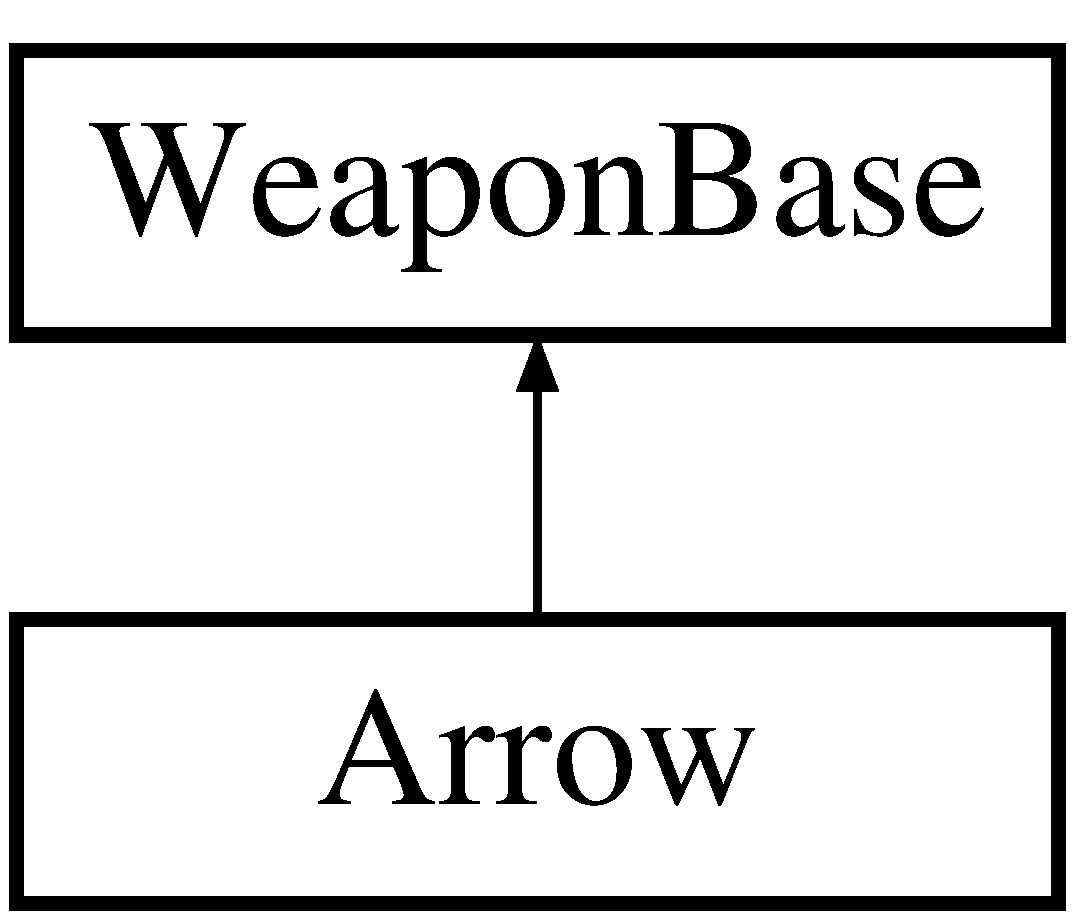
\includegraphics[height=2.000000cm]{class_arrow}
\end{center}
\end{figure}
\subsection*{公開メンバ関数}
\begin{DoxyCompactItemize}
\item 
void \mbox{\hyperlink{class_arrow_afe567fd69597c0a5c44edd99c06d6f71}{Collision\+Bullet}} ()
\begin{DoxyCompactList}\small\item\em 弾が当たったときに実行する関数 \end{DoxyCompactList}\item 
bool \mbox{\hyperlink{class_arrow_a98ea469bf0b21635b2d2dadb69c72240}{Attack}} (bool, const \mbox{\hyperlink{common_8h_ab1cb35b3a17c398d8ef71d5f779808bf}{Vec3}} \&) final
\begin{DoxyCompactList}\small\item\em 攻撃 \end{DoxyCompactList}\item 
void \mbox{\hyperlink{class_arrow_a085b5bd5f9e3ce25a081b502f9989f33}{Weapon\+Start}} () final
\begin{DoxyCompactList}\small\item\em 武器用の初期化 \end{DoxyCompactList}\item 
void \mbox{\hyperlink{class_arrow_afb6110035cba7b850d12755570163b29}{Weapon\+Update}} (const \mbox{\hyperlink{common_8h_ab1cb35b3a17c398d8ef71d5f779808bf}{Vec3}} \&, bool=true) final
\begin{DoxyCompactList}\small\item\em 武器の更新 \end{DoxyCompactList}\item 
void \mbox{\hyperlink{class_arrow_af9e54760156a77a15ad98a88f712ebdb}{Weapon\+Render}} (const \mbox{\hyperlink{common_8h_a1c43cb8f0d8a41901f3ce4c67dbbce20}{Transform}} \&=\mbox{\hyperlink{common_8h_a1c43cb8f0d8a41901f3ce4c67dbbce20}{Transform}}\{ saki\+::vector3\+\_\+zero$<$ float $>$, saki\+::vector3\+\_\+zero$<$ float $>$, saki\+::vector3\+\_\+zero$<$ float $>$ \}) final
\begin{DoxyCompactList}\small\item\em 武器の描画 \end{DoxyCompactList}\item 
void \mbox{\hyperlink{class_arrow_a1101d1159771b5c428afd3c7a6a0a4df}{Weapon\+Destroy}} () final
\begin{DoxyCompactList}\small\item\em 武器の破棄 \end{DoxyCompactList}\end{DoxyCompactItemize}
\subsection*{その他の継承メンバ}


\subsection{詳解}
遠距離武器クラス 

\subsection{関数詳解}
\mbox{\Hypertarget{class_arrow_a98ea469bf0b21635b2d2dadb69c72240}\label{class_arrow_a98ea469bf0b21635b2d2dadb69c72240}} 
\index{Arrow@{Arrow}!Attack@{Attack}}
\index{Attack@{Attack}!Arrow@{Arrow}}
\subsubsection{\texorpdfstring{Attack()}{Attack()}}
{\footnotesize\ttfamily bool Arrow\+::\+Attack (\begin{DoxyParamCaption}\item[{bool}]{right,  }\item[{const \mbox{\hyperlink{common_8h_ab1cb35b3a17c398d8ef71d5f779808bf}{Vec3}} \&}]{pos }\end{DoxyParamCaption})\hspace{0.3cm}{\ttfamily [final]}, {\ttfamily [virtual]}}



攻撃 


\begin{DoxyParams}{引数}
{\em right} & 右かどうか \\
\hline
{\em pos} & 弾を発射する位置 \\
\hline
\end{DoxyParams}


\mbox{\hyperlink{class_weapon_base_a1bab9c7fb9524db754bebbbcbf6c2fd9}{Weapon\+Base}}を実装しています。

\mbox{\Hypertarget{class_arrow_afe567fd69597c0a5c44edd99c06d6f71}\label{class_arrow_afe567fd69597c0a5c44edd99c06d6f71}} 
\index{Arrow@{Arrow}!Collision\+Bullet@{Collision\+Bullet}}
\index{Collision\+Bullet@{Collision\+Bullet}!Arrow@{Arrow}}
\subsubsection{\texorpdfstring{Collision\+Bullet()}{CollisionBullet()}}
{\footnotesize\ttfamily void Arrow\+::\+Collision\+Bullet (\begin{DoxyParamCaption}{ }\end{DoxyParamCaption})}



弾が当たったときに実行する関数 

\mbox{\Hypertarget{class_arrow_a1101d1159771b5c428afd3c7a6a0a4df}\label{class_arrow_a1101d1159771b5c428afd3c7a6a0a4df}} 
\index{Arrow@{Arrow}!Weapon\+Destroy@{Weapon\+Destroy}}
\index{Weapon\+Destroy@{Weapon\+Destroy}!Arrow@{Arrow}}
\subsubsection{\texorpdfstring{Weapon\+Destroy()}{WeaponDestroy()}}
{\footnotesize\ttfamily void Arrow\+::\+Weapon\+Destroy (\begin{DoxyParamCaption}{ }\end{DoxyParamCaption})\hspace{0.3cm}{\ttfamily [final]}, {\ttfamily [virtual]}}



武器の破棄 



\mbox{\hyperlink{class_weapon_base_a417784a8c8bf73cd398a77b922fc110c}{Weapon\+Base}}を実装しています。

\mbox{\Hypertarget{class_arrow_af9e54760156a77a15ad98a88f712ebdb}\label{class_arrow_af9e54760156a77a15ad98a88f712ebdb}} 
\index{Arrow@{Arrow}!Weapon\+Render@{Weapon\+Render}}
\index{Weapon\+Render@{Weapon\+Render}!Arrow@{Arrow}}
\subsubsection{\texorpdfstring{Weapon\+Render()}{WeaponRender()}}
{\footnotesize\ttfamily void Arrow\+::\+Weapon\+Render (\begin{DoxyParamCaption}\item[{const \mbox{\hyperlink{common_8h_a1c43cb8f0d8a41901f3ce4c67dbbce20}{Transform}} \&}]{ = {\ttfamily \mbox{\hyperlink{common_8h_a1c43cb8f0d8a41901f3ce4c67dbbce20}{Transform}}\{~saki\+:\+:vector3\+\_\+zero$<$float$>$,saki\+:\+:vector3\+\_\+zero$<$float$>$,saki\+:\+:vector3\+\_\+zero$<$float$>$~\}} }\end{DoxyParamCaption})\hspace{0.3cm}{\ttfamily [final]}, {\ttfamily [virtual]}}



武器の描画 


\begin{DoxyParams}{引数}
{\em t} & 描画位置 \\
\hline
\end{DoxyParams}


\mbox{\hyperlink{class_weapon_base_af308d16d3892c3ffaeedf74b08e761b9}{Weapon\+Base}}を実装しています。

\mbox{\Hypertarget{class_arrow_a085b5bd5f9e3ce25a081b502f9989f33}\label{class_arrow_a085b5bd5f9e3ce25a081b502f9989f33}} 
\index{Arrow@{Arrow}!Weapon\+Start@{Weapon\+Start}}
\index{Weapon\+Start@{Weapon\+Start}!Arrow@{Arrow}}
\subsubsection{\texorpdfstring{Weapon\+Start()}{WeaponStart()}}
{\footnotesize\ttfamily void Arrow\+::\+Weapon\+Start (\begin{DoxyParamCaption}{ }\end{DoxyParamCaption})\hspace{0.3cm}{\ttfamily [final]}, {\ttfamily [virtual]}}



武器用の初期化 



\mbox{\hyperlink{class_weapon_base_a25cd4c351638b76377e93341a9545712}{Weapon\+Base}}を実装しています。

\mbox{\Hypertarget{class_arrow_afb6110035cba7b850d12755570163b29}\label{class_arrow_afb6110035cba7b850d12755570163b29}} 
\index{Arrow@{Arrow}!Weapon\+Update@{Weapon\+Update}}
\index{Weapon\+Update@{Weapon\+Update}!Arrow@{Arrow}}
\subsubsection{\texorpdfstring{Weapon\+Update()}{WeaponUpdate()}}
{\footnotesize\ttfamily void Arrow\+::\+Weapon\+Update (\begin{DoxyParamCaption}\item[{const \mbox{\hyperlink{common_8h_ab1cb35b3a17c398d8ef71d5f779808bf}{Vec3}} \&}]{,  }\item[{bool}]{ = {\ttfamily true} }\end{DoxyParamCaption})\hspace{0.3cm}{\ttfamily [final]}, {\ttfamily [virtual]}}



武器の更新 



\mbox{\hyperlink{class_weapon_base_aa1e3d02353273ab72a71cc3a1563636a}{Weapon\+Base}}を実装しています。



このクラス詳解は次のファイルから抽出されました\+:\begin{DoxyCompactItemize}
\item 
C\+:/\+Users/tokir/\+Documents/\+Git\+Hub/\+Weapon\+Merchant\+Adventure/src/src/object/weapon/arrow/\mbox{\hyperlink{arrow_8h}{arrow.\+h}}\item 
C\+:/\+Users/tokir/\+Documents/\+Git\+Hub/\+Weapon\+Merchant\+Adventure/src/src/object/weapon/arrow/\mbox{\hyperlink{arrow_8cpp}{arrow.\+cpp}}\end{DoxyCompactItemize}

\hypertarget{class_bullet}{}\section{Bullet クラス}
\label{class_bullet}\index{Bullet@{Bullet}}


弾クラス  




{\ttfamily \#include $<$bullet.\+h$>$}

Bullet の継承関係図\begin{figure}[H]
\begin{center}
\leavevmode
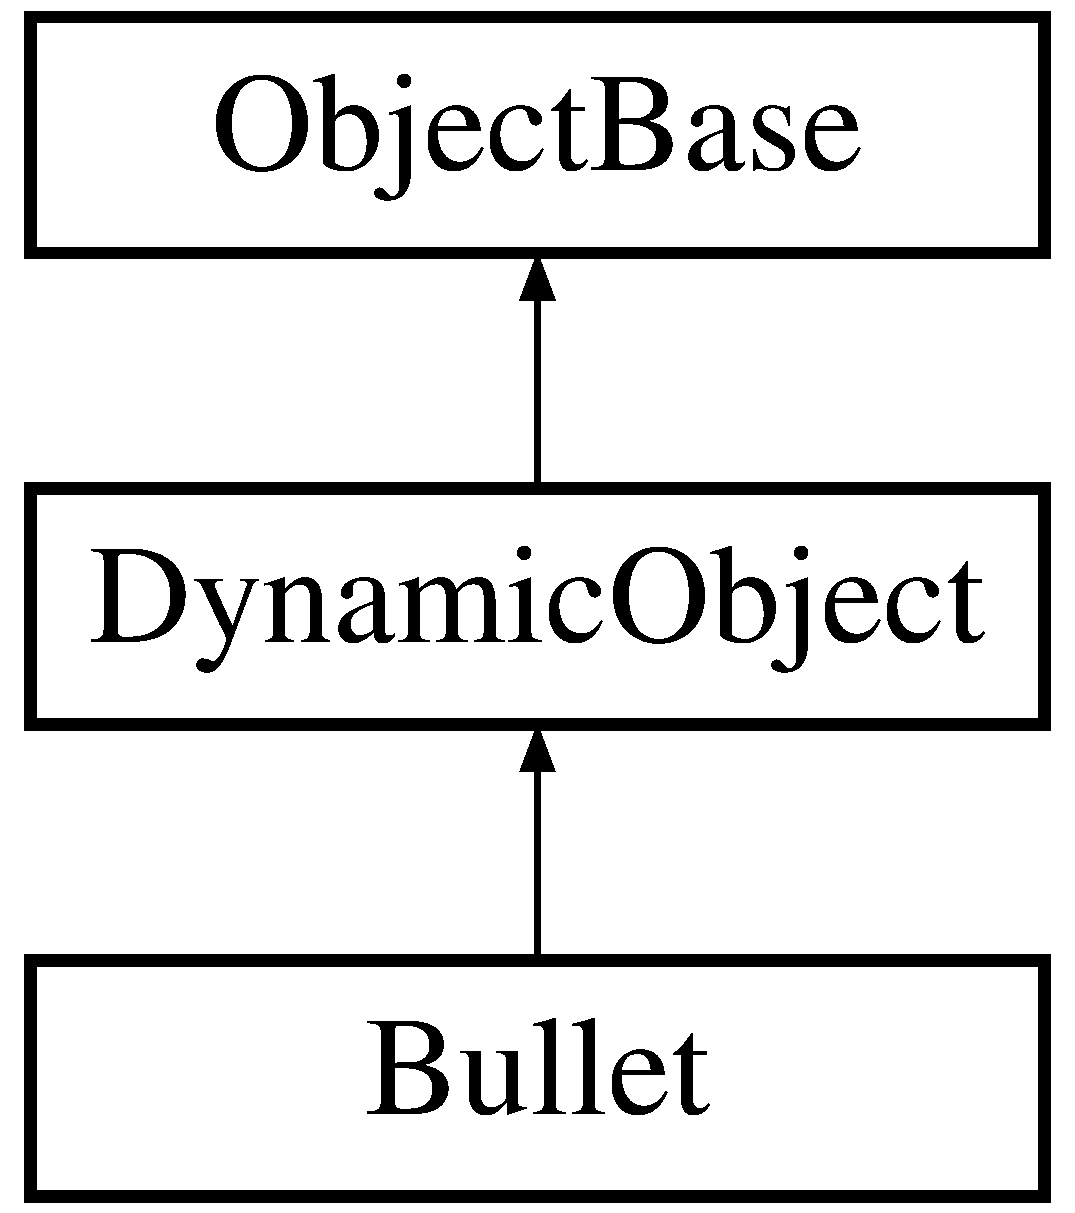
\includegraphics[height=3.000000cm]{class_bullet}
\end{center}
\end{figure}
\subsection*{公開メンバ関数}
\begin{DoxyCompactItemize}
\item 
\mbox{\hyperlink{class_bullet_acd7befc0bc18907cc1d871d37bbdddeb}{Bullet}} ()
\begin{DoxyCompactList}\small\item\em コンストラクタ \end{DoxyCompactList}\item 
\mbox{\hyperlink{class_bullet_a7e1ed7ba89e019b3d0fd068cfb4f9a6d}{Bullet}} (const \mbox{\hyperlink{class_bullet}{Bullet}} \&b)
\begin{DoxyCompactList}\small\item\em コピーコンストラクタ \end{DoxyCompactList}\item 
\mbox{\hyperlink{class_bullet}{Bullet}} \& \mbox{\hyperlink{class_bullet_a2a98443028be8389c0eb9da9a09f661c}{operator=}} (const \mbox{\hyperlink{class_bullet}{Bullet}} \&other)
\begin{DoxyCompactList}\small\item\em コピー代入演算子 \end{DoxyCompactList}\item 
\mbox{\hyperlink{class_bullet_a4bf8f227cde57a6abcdd268df2ef9a9d}{Bullet}} (\mbox{\hyperlink{class_bullet}{Bullet}} \&\&b)
\begin{DoxyCompactList}\small\item\em ムーブコンストラクタ \end{DoxyCompactList}\item 
void \mbox{\hyperlink{class_bullet_ab6b7b4ebc19095372a8e5ef3ad45ff65}{Bullet\+Init}} (const float, const std\+::function$<$ void()$>$ \&)
\begin{DoxyCompactList}\small\item\em 弾の初期化 \end{DoxyCompactList}\item 
void \mbox{\hyperlink{class_bullet_a09a92c6b924fb6bc38e18f6c41ac20ff}{Destroy}} () final
\begin{DoxyCompactList}\small\item\em 破棄 \end{DoxyCompactList}\item 
void \mbox{\hyperlink{class_bullet_a945da4a16d11cfee31139d564bea61f0}{Collision}} (\mbox{\hyperlink{class_object_base}{Object\+Base}} $\ast$, \mbox{\hyperlink{common_8h_afb0c5e21d4133ff4f200992c0b534e1b}{V\+E\+C2}}) final
\begin{DoxyCompactList}\small\item\em 当たったときに実行する関数 \end{DoxyCompactList}\item 
\mbox{\hyperlink{class_bullet_aaeb5cb41d7db89f49007b08b41f1bfcf}{$\sim$\+Bullet}} ()
\begin{DoxyCompactList}\small\item\em デストラクタ \end{DoxyCompactList}\end{DoxyCompactItemize}
\subsection*{限定公開メンバ関数}
\begin{DoxyCompactItemize}
\item 
void \mbox{\hyperlink{class_bullet_a448c1c566e002d7b51ba6ed5c927bff7}{Init\+Process}} () final
\begin{DoxyCompactList}\small\item\em 初期化 \end{DoxyCompactList}\item 
void \mbox{\hyperlink{class_bullet_aa0867038c9c35e30ee09e21ecdccf281}{Update\+Process}} () final
\begin{DoxyCompactList}\small\item\em 更新 \end{DoxyCompactList}\end{DoxyCompactItemize}
\subsection*{その他の継承メンバ}


\subsection{詳解}
弾クラス 

\subsection{構築子と解体子}
\mbox{\Hypertarget{class_bullet_acd7befc0bc18907cc1d871d37bbdddeb}\label{class_bullet_acd7befc0bc18907cc1d871d37bbdddeb}} 
\index{Bullet@{Bullet}!Bullet@{Bullet}}
\index{Bullet@{Bullet}!Bullet@{Bullet}}
\subsubsection{\texorpdfstring{Bullet()}{Bullet()}\hspace{0.1cm}{\footnotesize\ttfamily [1/3]}}
{\footnotesize\ttfamily Bullet\+::\+Bullet (\begin{DoxyParamCaption}{ }\end{DoxyParamCaption})\hspace{0.3cm}{\ttfamily [inline]}}



コンストラクタ 

\mbox{\Hypertarget{class_bullet_a7e1ed7ba89e019b3d0fd068cfb4f9a6d}\label{class_bullet_a7e1ed7ba89e019b3d0fd068cfb4f9a6d}} 
\index{Bullet@{Bullet}!Bullet@{Bullet}}
\index{Bullet@{Bullet}!Bullet@{Bullet}}
\subsubsection{\texorpdfstring{Bullet()}{Bullet()}\hspace{0.1cm}{\footnotesize\ttfamily [2/3]}}
{\footnotesize\ttfamily Bullet\+::\+Bullet (\begin{DoxyParamCaption}\item[{const \mbox{\hyperlink{class_bullet}{Bullet}} \&}]{b }\end{DoxyParamCaption})\hspace{0.3cm}{\ttfamily [inline]}}



コピーコンストラクタ 

\mbox{\Hypertarget{class_bullet_a4bf8f227cde57a6abcdd268df2ef9a9d}\label{class_bullet_a4bf8f227cde57a6abcdd268df2ef9a9d}} 
\index{Bullet@{Bullet}!Bullet@{Bullet}}
\index{Bullet@{Bullet}!Bullet@{Bullet}}
\subsubsection{\texorpdfstring{Bullet()}{Bullet()}\hspace{0.1cm}{\footnotesize\ttfamily [3/3]}}
{\footnotesize\ttfamily Bullet\+::\+Bullet (\begin{DoxyParamCaption}\item[{\mbox{\hyperlink{class_bullet}{Bullet}} \&\&}]{b }\end{DoxyParamCaption})\hspace{0.3cm}{\ttfamily [inline]}}



ムーブコンストラクタ 

\mbox{\Hypertarget{class_bullet_aaeb5cb41d7db89f49007b08b41f1bfcf}\label{class_bullet_aaeb5cb41d7db89f49007b08b41f1bfcf}} 
\index{Bullet@{Bullet}!````~Bullet@{$\sim$\+Bullet}}
\index{````~Bullet@{$\sim$\+Bullet}!Bullet@{Bullet}}
\subsubsection{\texorpdfstring{$\sim$\+Bullet()}{~Bullet()}}
{\footnotesize\ttfamily Bullet\+::$\sim$\+Bullet (\begin{DoxyParamCaption}{ }\end{DoxyParamCaption})\hspace{0.3cm}{\ttfamily [inline]}}



デストラクタ 



\subsection{関数詳解}
\mbox{\Hypertarget{class_bullet_ab6b7b4ebc19095372a8e5ef3ad45ff65}\label{class_bullet_ab6b7b4ebc19095372a8e5ef3ad45ff65}} 
\index{Bullet@{Bullet}!Bullet\+Init@{Bullet\+Init}}
\index{Bullet\+Init@{Bullet\+Init}!Bullet@{Bullet}}
\subsubsection{\texorpdfstring{Bullet\+Init()}{BulletInit()}}
{\footnotesize\ttfamily void Bullet\+::\+Bullet\+Init (\begin{DoxyParamCaption}\item[{const float}]{angle,  }\item[{const std\+::function$<$ void()$>$ \&}]{func }\end{DoxyParamCaption})}



弾の初期化 


\begin{DoxyParams}{引数}
{\em angle} & 発射角度 \\
\hline
{\em func} & 当たったときに実行する関数 \\
\hline
\end{DoxyParams}
\mbox{\Hypertarget{class_bullet_a945da4a16d11cfee31139d564bea61f0}\label{class_bullet_a945da4a16d11cfee31139d564bea61f0}} 
\index{Bullet@{Bullet}!Collision@{Collision}}
\index{Collision@{Collision}!Bullet@{Bullet}}
\subsubsection{\texorpdfstring{Collision()}{Collision()}}
{\footnotesize\ttfamily void Bullet\+::\+Collision (\begin{DoxyParamCaption}\item[{\mbox{\hyperlink{class_object_base}{Object\+Base}} $\ast$}]{obj,  }\item[{\mbox{\hyperlink{common_8h_afb0c5e21d4133ff4f200992c0b534e1b}{V\+E\+C2}}}]{ }\end{DoxyParamCaption})\hspace{0.3cm}{\ttfamily [final]}, {\ttfamily [virtual]}}



当たったときに実行する関数 


\begin{DoxyParams}{引数}
{\em obj} & 当たった相手のオブジェクト \\
\hline
\end{DoxyParams}


\mbox{\hyperlink{class_object_base_ad772d7a42f5e46c39481f5db22ee8193}{Object\+Base}}を再実装しています。

\mbox{\Hypertarget{class_bullet_a09a92c6b924fb6bc38e18f6c41ac20ff}\label{class_bullet_a09a92c6b924fb6bc38e18f6c41ac20ff}} 
\index{Bullet@{Bullet}!Destroy@{Destroy}}
\index{Destroy@{Destroy}!Bullet@{Bullet}}
\subsubsection{\texorpdfstring{Destroy()}{Destroy()}}
{\footnotesize\ttfamily void Bullet\+::\+Destroy (\begin{DoxyParamCaption}{ }\end{DoxyParamCaption})\hspace{0.3cm}{\ttfamily [final]}, {\ttfamily [virtual]}}



破棄 



\mbox{\hyperlink{class_object_base_a7fa4c548153c3af20f89673ffea809af}{Object\+Base}}を実装しています。

\mbox{\Hypertarget{class_bullet_a448c1c566e002d7b51ba6ed5c927bff7}\label{class_bullet_a448c1c566e002d7b51ba6ed5c927bff7}} 
\index{Bullet@{Bullet}!Init\+Process@{Init\+Process}}
\index{Init\+Process@{Init\+Process}!Bullet@{Bullet}}
\subsubsection{\texorpdfstring{Init\+Process()}{InitProcess()}}
{\footnotesize\ttfamily void Bullet\+::\+Init\+Process (\begin{DoxyParamCaption}{ }\end{DoxyParamCaption})\hspace{0.3cm}{\ttfamily [final]}, {\ttfamily [protected]}, {\ttfamily [virtual]}}



初期化 



\mbox{\hyperlink{class_object_base_af133f36f2bca1dcfd962e2cfac61ab51}{Object\+Base}}を実装しています。

\mbox{\Hypertarget{class_bullet_a2a98443028be8389c0eb9da9a09f661c}\label{class_bullet_a2a98443028be8389c0eb9da9a09f661c}} 
\index{Bullet@{Bullet}!operator=@{operator=}}
\index{operator=@{operator=}!Bullet@{Bullet}}
\subsubsection{\texorpdfstring{operator=()}{operator=()}}
{\footnotesize\ttfamily \mbox{\hyperlink{class_bullet}{Bullet}}\& Bullet\+::operator= (\begin{DoxyParamCaption}\item[{const \mbox{\hyperlink{class_bullet}{Bullet}} \&}]{other }\end{DoxyParamCaption})\hspace{0.3cm}{\ttfamily [inline]}}



コピー代入演算子 

\mbox{\Hypertarget{class_bullet_aa0867038c9c35e30ee09e21ecdccf281}\label{class_bullet_aa0867038c9c35e30ee09e21ecdccf281}} 
\index{Bullet@{Bullet}!Update\+Process@{Update\+Process}}
\index{Update\+Process@{Update\+Process}!Bullet@{Bullet}}
\subsubsection{\texorpdfstring{Update\+Process()}{UpdateProcess()}}
{\footnotesize\ttfamily void Bullet\+::\+Update\+Process (\begin{DoxyParamCaption}{ }\end{DoxyParamCaption})\hspace{0.3cm}{\ttfamily [final]}, {\ttfamily [protected]}, {\ttfamily [virtual]}}



更新 



\mbox{\hyperlink{class_object_base_a8b5b72b363a419767efde0b0e692ea95}{Object\+Base}}を実装しています。



このクラス詳解は次のファイルから抽出されました\+:\begin{DoxyCompactItemize}
\item 
C\+:/\+Users/tokir/\+Documents/\+Git\+Hub/\+Weapon\+Merchant\+Adventure/src/object/weapon/arrow/bullet/\mbox{\hyperlink{bullet_8h}{bullet.\+h}}\item 
C\+:/\+Users/tokir/\+Documents/\+Git\+Hub/\+Weapon\+Merchant\+Adventure/src/object/weapon/arrow/bullet/\mbox{\hyperlink{bullet_8cpp}{bullet.\+cpp}}\end{DoxyCompactItemize}

\hypertarget{class_camera}{}\section{Camera クラス}
\label{class_camera}\index{Camera@{Camera}}


カメラクラス  




{\ttfamily \#include $<$camera.\+h$>$}

Camera の継承関係図\begin{figure}[H]
\begin{center}
\leavevmode
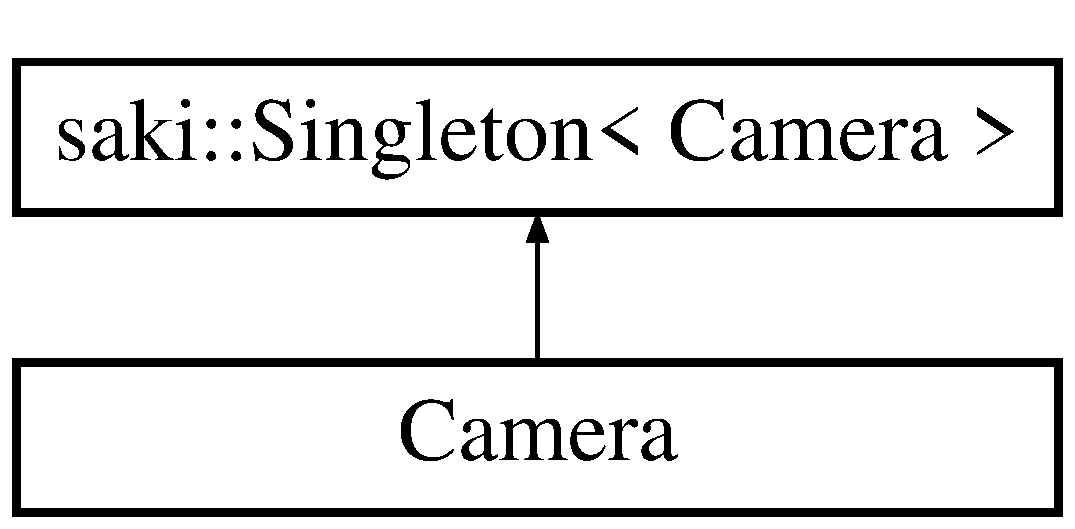
\includegraphics[height=2.000000cm]{class_camera}
\end{center}
\end{figure}
\subsection*{公開メンバ関数}
\begin{DoxyCompactItemize}
\item 
\mbox{\hyperlink{class_camera_a01f94c3543f56ede7af49dc778f19331}{Camera}} ()
\item 
\mbox{\hyperlink{class_camera_afe282ee51f1f39c041b0e7de9386cc6d}{Camera}} (const \mbox{\hyperlink{common_8h_afb0c5e21d4133ff4f200992c0b534e1b}{V\+E\+C2}} \&)
\begin{DoxyCompactList}\small\item\em カメラの値を受け取る初期化コンストラクタ \end{DoxyCompactList}\item 
void \mbox{\hyperlink{class_camera_a5c6b7ad424d835a3022393099886a90b}{Move}} (const \mbox{\hyperlink{common_8h_afb0c5e21d4133ff4f200992c0b534e1b}{V\+E\+C2}} \&)
\begin{DoxyCompactList}\small\item\em カメラの移動 \end{DoxyCompactList}\item 
void \mbox{\hyperlink{class_camera_af79aa3fedd030712e7fa122a2ea88b48}{Set\+Pos}} (const \mbox{\hyperlink{common_8h_afb0c5e21d4133ff4f200992c0b534e1b}{V\+E\+C2}} \&)
\begin{DoxyCompactList}\small\item\em カメラの位置変更 \end{DoxyCompactList}\item 
\mbox{\hyperlink{common_8h_afb0c5e21d4133ff4f200992c0b534e1b}{V\+E\+C2}} \mbox{\hyperlink{class_camera_ac3b4f1248489c0ac0faa521329de71cd}{Get\+Pos}} () const
\begin{DoxyCompactList}\small\item\em カメラの位置を取得 \end{DoxyCompactList}\item 
void \mbox{\hyperlink{class_camera_a4a596a3ea1fdc7d244ba4268031a360b}{Update}} ()
\begin{DoxyCompactList}\small\item\em カメラの更新 \end{DoxyCompactList}\item 
void \mbox{\hyperlink{class_camera_a7336f8f6c9145bee1ce6b1f16f0aaee4}{Set\+Target}} (\mbox{\hyperlink{class_object_base}{Object\+Base}} $\ast$t)
\end{DoxyCompactItemize}
\subsection*{その他の継承メンバ}


\subsection{詳解}
カメラクラス 

\subsection{構築子と解体子}
\mbox{\Hypertarget{class_camera_a01f94c3543f56ede7af49dc778f19331}\label{class_camera_a01f94c3543f56ede7af49dc778f19331}} 
\index{Camera@{Camera}!Camera@{Camera}}
\index{Camera@{Camera}!Camera@{Camera}}
\subsubsection{\texorpdfstring{Camera()}{Camera()}\hspace{0.1cm}{\footnotesize\ttfamily [1/2]}}
{\footnotesize\ttfamily Camera\+::\+Camera (\begin{DoxyParamCaption}{ }\end{DoxyParamCaption})\hspace{0.3cm}{\ttfamily [inline]}}

\mbox{\Hypertarget{class_camera_afe282ee51f1f39c041b0e7de9386cc6d}\label{class_camera_afe282ee51f1f39c041b0e7de9386cc6d}} 
\index{Camera@{Camera}!Camera@{Camera}}
\index{Camera@{Camera}!Camera@{Camera}}
\subsubsection{\texorpdfstring{Camera()}{Camera()}\hspace{0.1cm}{\footnotesize\ttfamily [2/2]}}
{\footnotesize\ttfamily Camera\+::\+Camera (\begin{DoxyParamCaption}\item[{const \mbox{\hyperlink{common_8h_afb0c5e21d4133ff4f200992c0b534e1b}{V\+E\+C2}} \&}]{v2 }\end{DoxyParamCaption})}



カメラの値を受け取る初期化コンストラクタ 


\begin{DoxyParams}{引数}
{\em v2} & 初期化する値 \\
\hline
\end{DoxyParams}


\subsection{関数詳解}
\mbox{\Hypertarget{class_camera_ac3b4f1248489c0ac0faa521329de71cd}\label{class_camera_ac3b4f1248489c0ac0faa521329de71cd}} 
\index{Camera@{Camera}!Get\+Pos@{Get\+Pos}}
\index{Get\+Pos@{Get\+Pos}!Camera@{Camera}}
\subsubsection{\texorpdfstring{Get\+Pos()}{GetPos()}}
{\footnotesize\ttfamily \mbox{\hyperlink{common_8h_afb0c5e21d4133ff4f200992c0b534e1b}{V\+E\+C2}} Camera\+::\+Get\+Pos (\begin{DoxyParamCaption}{ }\end{DoxyParamCaption}) const}



カメラの位置を取得 

\begin{DoxyReturn}{戻り値}
V\+E\+C2\+:カメラの位置 
\end{DoxyReturn}
\mbox{\Hypertarget{class_camera_a5c6b7ad424d835a3022393099886a90b}\label{class_camera_a5c6b7ad424d835a3022393099886a90b}} 
\index{Camera@{Camera}!Move@{Move}}
\index{Move@{Move}!Camera@{Camera}}
\subsubsection{\texorpdfstring{Move()}{Move()}}
{\footnotesize\ttfamily void Camera\+::\+Move (\begin{DoxyParamCaption}\item[{const \mbox{\hyperlink{common_8h_afb0c5e21d4133ff4f200992c0b534e1b}{V\+E\+C2}} \&}]{v2 }\end{DoxyParamCaption})}



カメラの移動 


\begin{DoxyParams}{引数}
{\em v2} & 移動量 \\
\hline
\end{DoxyParams}
\mbox{\Hypertarget{class_camera_af79aa3fedd030712e7fa122a2ea88b48}\label{class_camera_af79aa3fedd030712e7fa122a2ea88b48}} 
\index{Camera@{Camera}!Set\+Pos@{Set\+Pos}}
\index{Set\+Pos@{Set\+Pos}!Camera@{Camera}}
\subsubsection{\texorpdfstring{Set\+Pos()}{SetPos()}}
{\footnotesize\ttfamily void Camera\+::\+Set\+Pos (\begin{DoxyParamCaption}\item[{const \mbox{\hyperlink{common_8h_afb0c5e21d4133ff4f200992c0b534e1b}{V\+E\+C2}} \&}]{v2 }\end{DoxyParamCaption})}



カメラの位置変更 


\begin{DoxyParams}{引数}
{\em v2} & 位置 \\
\hline
\end{DoxyParams}
\mbox{\Hypertarget{class_camera_a7336f8f6c9145bee1ce6b1f16f0aaee4}\label{class_camera_a7336f8f6c9145bee1ce6b1f16f0aaee4}} 
\index{Camera@{Camera}!Set\+Target@{Set\+Target}}
\index{Set\+Target@{Set\+Target}!Camera@{Camera}}
\subsubsection{\texorpdfstring{Set\+Target()}{SetTarget()}}
{\footnotesize\ttfamily void Camera\+::\+Set\+Target (\begin{DoxyParamCaption}\item[{\mbox{\hyperlink{class_object_base}{Object\+Base}} $\ast$}]{t }\end{DoxyParamCaption})\hspace{0.3cm}{\ttfamily [inline]}}

brief ターゲットのセット \mbox{\Hypertarget{class_camera_a4a596a3ea1fdc7d244ba4268031a360b}\label{class_camera_a4a596a3ea1fdc7d244ba4268031a360b}} 
\index{Camera@{Camera}!Update@{Update}}
\index{Update@{Update}!Camera@{Camera}}
\subsubsection{\texorpdfstring{Update()}{Update()}}
{\footnotesize\ttfamily void Camera\+::\+Update (\begin{DoxyParamCaption}{ }\end{DoxyParamCaption})}



カメラの更新 



このクラス詳解は次のファイルから抽出されました\+:\begin{DoxyCompactItemize}
\item 
C\+:/\+Users/tokir/\+Documents/\+Git\+Hub/\+Weapon\+Merchant\+Adventure/src/object/camera/\mbox{\hyperlink{camera_8h}{camera.\+h}}\item 
C\+:/\+Users/tokir/\+Documents/\+Git\+Hub/\+Weapon\+Merchant\+Adventure/src/object/camera/\mbox{\hyperlink{camera_8cpp}{camera.\+cpp}}\end{DoxyCompactItemize}

\hypertarget{class_collider_base}{}\section{Collider\+Base クラス}
\label{class_collider_base}\index{Collider\+Base@{Collider\+Base}}


コライダのスーパークラス  




{\ttfamily \#include $<$collider\+\_\+base.\+h$>$}

Collider\+Base の継承関係図\begin{figure}[H]
\begin{center}
\leavevmode
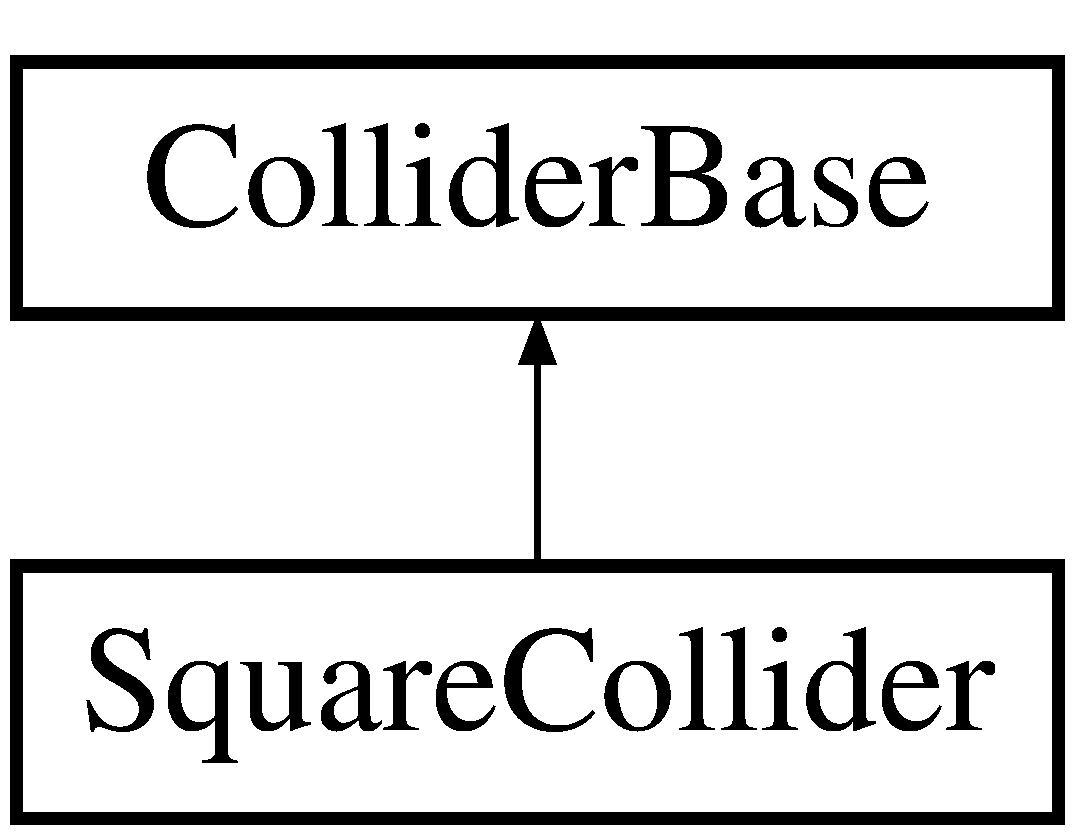
\includegraphics[height=2.000000cm]{class_collider_base}
\end{center}
\end{figure}
\subsection*{公開メンバ関数}
\begin{DoxyCompactItemize}
\item 
\mbox{\hyperlink{class_collider_base_a61d7057a7e05549088f2b15c1e525858}{Collider\+Base}} (\mbox{\hyperlink{class_object_base}{Object\+Base}} $\ast$obj, bool \+\_\+is\+\_\+trigger=false)
\begin{DoxyCompactList}\small\item\em コンストラクタ \end{DoxyCompactList}\item 
\mbox{\hyperlink{class_collider_base}{Collider\+Base}} \& \mbox{\hyperlink{class_collider_base_a2bc4d08eb29126c0cb0ea45b06517328}{operator=}} (const \mbox{\hyperlink{class_collider_base}{Collider\+Base}} \&other)
\begin{DoxyCompactList}\small\item\em コピー代入演算子 \end{DoxyCompactList}\item 
virtual \mbox{\hyperlink{class_collider_base_a485c8a6348a053228aa61142a71e48fb}{$\sim$\+Collider\+Base}} ()
\end{DoxyCompactItemize}
\subsection*{公開変数類}
\begin{DoxyCompactItemize}
\item 
bool \mbox{\hyperlink{class_collider_base_a1943a8429f6ef2cce5785975cba321b1}{collision\+\_\+destroy}} = false
\item 
bool \mbox{\hyperlink{class_collider_base_a8e2383d9422880103aa5309a6dfcef48}{is\+\_\+trigger}}
\item 
bool \mbox{\hyperlink{class_collider_base_a7e6348c051a8c01ff7884d366bd292eb}{collision\+\_\+is\+\_\+static\+\_\+x}} = false
\item 
bool \mbox{\hyperlink{class_collider_base_a5a50a0f911a108eba730de1b22c1cc9e}{collision\+\_\+is\+\_\+static\+\_\+y}} = false
\item 
\mbox{\hyperlink{class_object_base}{Object\+Base}} $\ast$ \mbox{\hyperlink{class_collider_base_a63adac6a75877857abe9ff2cf4274157}{object}}
\item 
std\+::function$<$ void(\mbox{\hyperlink{class_object_base}{Object\+Base}} $\ast$, \mbox{\hyperlink{common_8h_afb0c5e21d4133ff4f200992c0b534e1b}{V\+E\+C2}})$>$ \mbox{\hyperlink{class_collider_base_a5ac4f3c76c753790abef75e3eb7accbe}{collision\+\_\+func}}
\item 
bool \mbox{\hyperlink{class_collider_base_a812053f247dc6357357bdf9353dded77}{enabled}} = true
\end{DoxyCompactItemize}


\subsection{詳解}
コライダのスーパークラス 

\subsection{構築子と解体子}
\mbox{\Hypertarget{class_collider_base_a61d7057a7e05549088f2b15c1e525858}\label{class_collider_base_a61d7057a7e05549088f2b15c1e525858}} 
\index{Collider\+Base@{Collider\+Base}!Collider\+Base@{Collider\+Base}}
\index{Collider\+Base@{Collider\+Base}!Collider\+Base@{Collider\+Base}}
\subsubsection{\texorpdfstring{Collider\+Base()}{ColliderBase()}}
{\footnotesize\ttfamily Collider\+Base\+::\+Collider\+Base (\begin{DoxyParamCaption}\item[{\mbox{\hyperlink{class_object_base}{Object\+Base}} $\ast$}]{obj,  }\item[{bool}]{\+\_\+is\+\_\+trigger = {\ttfamily false} }\end{DoxyParamCaption})\hspace{0.3cm}{\ttfamily [inline]}}



コンストラクタ 


\begin{DoxyParams}{引数}
{\em obj} & オブジェクト \\
\hline
{\em \+\_\+is\+\_\+trigger} & 押し出しするかどうか \\
\hline
\end{DoxyParams}
\mbox{\Hypertarget{class_collider_base_a485c8a6348a053228aa61142a71e48fb}\label{class_collider_base_a485c8a6348a053228aa61142a71e48fb}} 
\index{Collider\+Base@{Collider\+Base}!````~Collider\+Base@{$\sim$\+Collider\+Base}}
\index{````~Collider\+Base@{$\sim$\+Collider\+Base}!Collider\+Base@{Collider\+Base}}
\subsubsection{\texorpdfstring{$\sim$\+Collider\+Base()}{~ColliderBase()}}
{\footnotesize\ttfamily virtual Collider\+Base\+::$\sim$\+Collider\+Base (\begin{DoxyParamCaption}{ }\end{DoxyParamCaption})\hspace{0.3cm}{\ttfamily [inline]}, {\ttfamily [virtual]}}



\subsection{関数詳解}
\mbox{\Hypertarget{class_collider_base_a2bc4d08eb29126c0cb0ea45b06517328}\label{class_collider_base_a2bc4d08eb29126c0cb0ea45b06517328}} 
\index{Collider\+Base@{Collider\+Base}!operator=@{operator=}}
\index{operator=@{operator=}!Collider\+Base@{Collider\+Base}}
\subsubsection{\texorpdfstring{operator=()}{operator=()}}
{\footnotesize\ttfamily \mbox{\hyperlink{class_collider_base}{Collider\+Base}}\& Collider\+Base\+::operator= (\begin{DoxyParamCaption}\item[{const \mbox{\hyperlink{class_collider_base}{Collider\+Base}} \&}]{other }\end{DoxyParamCaption})\hspace{0.3cm}{\ttfamily [inline]}}



コピー代入演算子 



\subsection{メンバ詳解}
\mbox{\Hypertarget{class_collider_base_a1943a8429f6ef2cce5785975cba321b1}\label{class_collider_base_a1943a8429f6ef2cce5785975cba321b1}} 
\index{Collider\+Base@{Collider\+Base}!collision\+\_\+destroy@{collision\+\_\+destroy}}
\index{collision\+\_\+destroy@{collision\+\_\+destroy}!Collider\+Base@{Collider\+Base}}
\subsubsection{\texorpdfstring{collision\+\_\+destroy}{collision\_destroy}}
{\footnotesize\ttfamily bool Collider\+Base\+::collision\+\_\+destroy = false}

\mbox{\Hypertarget{class_collider_base_a5ac4f3c76c753790abef75e3eb7accbe}\label{class_collider_base_a5ac4f3c76c753790abef75e3eb7accbe}} 
\index{Collider\+Base@{Collider\+Base}!collision\+\_\+func@{collision\+\_\+func}}
\index{collision\+\_\+func@{collision\+\_\+func}!Collider\+Base@{Collider\+Base}}
\subsubsection{\texorpdfstring{collision\+\_\+func}{collision\_func}}
{\footnotesize\ttfamily std\+::function$<$void(\mbox{\hyperlink{class_object_base}{Object\+Base}}$\ast$,\mbox{\hyperlink{common_8h_afb0c5e21d4133ff4f200992c0b534e1b}{V\+E\+C2}})$>$ Collider\+Base\+::collision\+\_\+func}

\mbox{\Hypertarget{class_collider_base_a7e6348c051a8c01ff7884d366bd292eb}\label{class_collider_base_a7e6348c051a8c01ff7884d366bd292eb}} 
\index{Collider\+Base@{Collider\+Base}!collision\+\_\+is\+\_\+static\+\_\+x@{collision\+\_\+is\+\_\+static\+\_\+x}}
\index{collision\+\_\+is\+\_\+static\+\_\+x@{collision\+\_\+is\+\_\+static\+\_\+x}!Collider\+Base@{Collider\+Base}}
\subsubsection{\texorpdfstring{collision\+\_\+is\+\_\+static\+\_\+x}{collision\_is\_static\_x}}
{\footnotesize\ttfamily bool Collider\+Base\+::collision\+\_\+is\+\_\+static\+\_\+x = false}

\mbox{\Hypertarget{class_collider_base_a5a50a0f911a108eba730de1b22c1cc9e}\label{class_collider_base_a5a50a0f911a108eba730de1b22c1cc9e}} 
\index{Collider\+Base@{Collider\+Base}!collision\+\_\+is\+\_\+static\+\_\+y@{collision\+\_\+is\+\_\+static\+\_\+y}}
\index{collision\+\_\+is\+\_\+static\+\_\+y@{collision\+\_\+is\+\_\+static\+\_\+y}!Collider\+Base@{Collider\+Base}}
\subsubsection{\texorpdfstring{collision\+\_\+is\+\_\+static\+\_\+y}{collision\_is\_static\_y}}
{\footnotesize\ttfamily bool Collider\+Base\+::collision\+\_\+is\+\_\+static\+\_\+y = false}

\mbox{\Hypertarget{class_collider_base_a812053f247dc6357357bdf9353dded77}\label{class_collider_base_a812053f247dc6357357bdf9353dded77}} 
\index{Collider\+Base@{Collider\+Base}!enabled@{enabled}}
\index{enabled@{enabled}!Collider\+Base@{Collider\+Base}}
\subsubsection{\texorpdfstring{enabled}{enabled}}
{\footnotesize\ttfamily bool Collider\+Base\+::enabled = true}

\mbox{\Hypertarget{class_collider_base_a8e2383d9422880103aa5309a6dfcef48}\label{class_collider_base_a8e2383d9422880103aa5309a6dfcef48}} 
\index{Collider\+Base@{Collider\+Base}!is\+\_\+trigger@{is\+\_\+trigger}}
\index{is\+\_\+trigger@{is\+\_\+trigger}!Collider\+Base@{Collider\+Base}}
\subsubsection{\texorpdfstring{is\+\_\+trigger}{is\_trigger}}
{\footnotesize\ttfamily bool Collider\+Base\+::is\+\_\+trigger}

\mbox{\Hypertarget{class_collider_base_a63adac6a75877857abe9ff2cf4274157}\label{class_collider_base_a63adac6a75877857abe9ff2cf4274157}} 
\index{Collider\+Base@{Collider\+Base}!object@{object}}
\index{object@{object}!Collider\+Base@{Collider\+Base}}
\subsubsection{\texorpdfstring{object}{object}}
{\footnotesize\ttfamily \mbox{\hyperlink{class_object_base}{Object\+Base}}$\ast$ Collider\+Base\+::object}



このクラス詳解は次のファイルから抽出されました\+:\begin{DoxyCompactItemize}
\item 
C\+:/\+Users/tokir/\+Documents/\+Git\+Hub/\+Weapon\+Merchant\+Adventure/src/collider/base/\mbox{\hyperlink{collider__base_8h}{collider\+\_\+base.\+h}}\end{DoxyCompactItemize}

\hypertarget{class_collider_manager}{}\section{Collider\+Manager クラス}
\label{class_collider_manager}\index{Collider\+Manager@{Collider\+Manager}}


コライダを管理するクラス  




{\ttfamily \#include $<$collider\+\_\+manager.\+h$>$}

Collider\+Manager の継承関係図\begin{figure}[H]
\begin{center}
\leavevmode
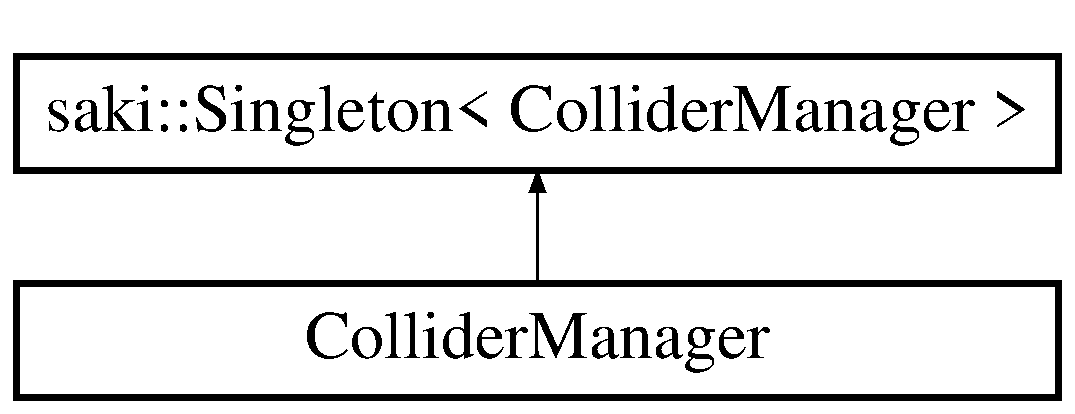
\includegraphics[height=2.000000cm]{class_collider_manager}
\end{center}
\end{figure}
\subsection*{公開メンバ関数}
\begin{DoxyCompactItemize}
\item 
void \mbox{\hyperlink{class_collider_manager_a9e6c7ca21ae4e79fdf4892982e72bc99}{Set\+Square\+Collider}} (\mbox{\hyperlink{class_square_collider}{Square\+Collider}} $\ast$, bool is\+\_\+static)
\begin{DoxyCompactList}\small\item\em コライダを配列に格納する \end{DoxyCompactList}\item 
void \mbox{\hyperlink{class_collider_manager_af3863143e206b4c86c8b89dd91ff3c8c}{Check\+Collision}} ()
\begin{DoxyCompactList}\small\item\em 全てのコライダを走査する \end{DoxyCompactList}\item 
void \mbox{\hyperlink{class_collider_manager_a24df637a6f092602b547c6a2bd773113}{Delete\+Square\+Collider}} (\mbox{\hyperlink{class_square_collider}{Square\+Collider}} $\ast$)
\begin{DoxyCompactList}\small\item\em 四角形コライダの削除 \end{DoxyCompactList}\end{DoxyCompactItemize}
\subsection*{限定公開メンバ関数}
\begin{DoxyCompactItemize}
\item 
bool \mbox{\hyperlink{class_collider_manager_a612f6096ca24702bff6dee04a88a40c3}{Compare\+Square\+Square\+Collision}} (const \mbox{\hyperlink{class_square_collider}{Square\+Collider}} $\ast$, const \mbox{\hyperlink{class_square_collider}{Square\+Collider}} $\ast$)
\begin{DoxyCompactList}\small\item\em 四角形同士が当たっているかを判定する \end{DoxyCompactList}\end{DoxyCompactItemize}
\subsection*{その他の継承メンバ}


\subsection{詳解}
コライダを管理するクラス 

\subsection{関数詳解}
\mbox{\Hypertarget{class_collider_manager_af3863143e206b4c86c8b89dd91ff3c8c}\label{class_collider_manager_af3863143e206b4c86c8b89dd91ff3c8c}} 
\index{Collider\+Manager@{Collider\+Manager}!Check\+Collision@{Check\+Collision}}
\index{Check\+Collision@{Check\+Collision}!Collider\+Manager@{Collider\+Manager}}
\subsubsection{\texorpdfstring{Check\+Collision()}{CheckCollision()}}
{\footnotesize\ttfamily void Collider\+Manager\+::\+Check\+Collision (\begin{DoxyParamCaption}{ }\end{DoxyParamCaption})}



全てのコライダを走査する 

\mbox{\Hypertarget{class_collider_manager_a612f6096ca24702bff6dee04a88a40c3}\label{class_collider_manager_a612f6096ca24702bff6dee04a88a40c3}} 
\index{Collider\+Manager@{Collider\+Manager}!Compare\+Square\+Square\+Collision@{Compare\+Square\+Square\+Collision}}
\index{Compare\+Square\+Square\+Collision@{Compare\+Square\+Square\+Collision}!Collider\+Manager@{Collider\+Manager}}
\subsubsection{\texorpdfstring{Compare\+Square\+Square\+Collision()}{CompareSquareSquareCollision()}}
{\footnotesize\ttfamily bool Collider\+Manager\+::\+Compare\+Square\+Square\+Collision (\begin{DoxyParamCaption}\item[{const \mbox{\hyperlink{class_square_collider}{Square\+Collider}} $\ast$}]{col1,  }\item[{const \mbox{\hyperlink{class_square_collider}{Square\+Collider}} $\ast$}]{col2 }\end{DoxyParamCaption})\hspace{0.3cm}{\ttfamily [protected]}}



四角形同士が当たっているかを判定する 


\begin{DoxyParams}{引数}
{\em col1,col2} & 比べる二つの四角形コライダ \\
\hline
\end{DoxyParams}
\begin{DoxyReturn}{戻り値}
bool 当たっているかどうか 
\end{DoxyReturn}
\mbox{\Hypertarget{class_collider_manager_a24df637a6f092602b547c6a2bd773113}\label{class_collider_manager_a24df637a6f092602b547c6a2bd773113}} 
\index{Collider\+Manager@{Collider\+Manager}!Delete\+Square\+Collider@{Delete\+Square\+Collider}}
\index{Delete\+Square\+Collider@{Delete\+Square\+Collider}!Collider\+Manager@{Collider\+Manager}}
\subsubsection{\texorpdfstring{Delete\+Square\+Collider()}{DeleteSquareCollider()}}
{\footnotesize\ttfamily void Collider\+Manager\+::\+Delete\+Square\+Collider (\begin{DoxyParamCaption}\item[{\mbox{\hyperlink{class_square_collider}{Square\+Collider}} $\ast$}]{col }\end{DoxyParamCaption})}



四角形コライダの削除 


\begin{DoxyParams}{引数}
{\em col} & 四角形コライダ \\
\hline
\end{DoxyParams}
\mbox{\Hypertarget{class_collider_manager_a9e6c7ca21ae4e79fdf4892982e72bc99}\label{class_collider_manager_a9e6c7ca21ae4e79fdf4892982e72bc99}} 
\index{Collider\+Manager@{Collider\+Manager}!Set\+Square\+Collider@{Set\+Square\+Collider}}
\index{Set\+Square\+Collider@{Set\+Square\+Collider}!Collider\+Manager@{Collider\+Manager}}
\subsubsection{\texorpdfstring{Set\+Square\+Collider()}{SetSquareCollider()}}
{\footnotesize\ttfamily void Collider\+Manager\+::\+Set\+Square\+Collider (\begin{DoxyParamCaption}\item[{\mbox{\hyperlink{class_square_collider}{Square\+Collider}} $\ast$}]{obj,  }\item[{bool}]{is\+\_\+static }\end{DoxyParamCaption})}



コライダを配列に格納する 


\begin{DoxyParams}{引数}
{\em obj} & 当たり判定クラス \\
\hline
{\em is\+\_\+static} & 静的か動的か \\
\hline
\end{DoxyParams}


このクラス詳解は次のファイルから抽出されました\+:\begin{DoxyCompactItemize}
\item 
C\+:/\+Users/tokir/\+Documents/\+Git\+Hub/\+Weapon\+Merchant\+Adventure/src/collider/manager/\mbox{\hyperlink{collider__manager_8h}{collider\+\_\+manager.\+h}}\item 
C\+:/\+Users/tokir/\+Documents/\+Git\+Hub/\+Weapon\+Merchant\+Adventure/src/collider/manager/\mbox{\hyperlink{collider__manager_8cpp}{collider\+\_\+manager.\+cpp}}\end{DoxyCompactItemize}

\hypertarget{class_dynamic_object}{}\section{Dynamic\+Object クラス}
\label{class_dynamic_object}\index{Dynamic\+Object@{Dynamic\+Object}}


動くオブジェクトのスーパークラス  




{\ttfamily \#include $<$dynamic\+\_\+object.\+h$>$}

Dynamic\+Object の継承関係図\begin{figure}[H]
\begin{center}
\leavevmode
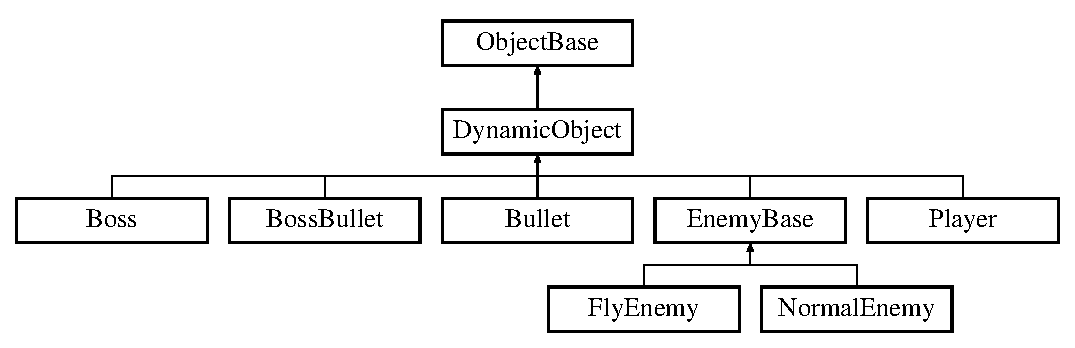
\includegraphics[height=4.000000cm]{class_dynamic_object}
\end{center}
\end{figure}
\subsection*{公開メンバ関数}
\begin{DoxyCompactItemize}
\item 
\mbox{\hyperlink{class_dynamic_object_a50a7adf3d7d1f411ed2aa9a663bfe275}{Dynamic\+Object}} ()
\begin{DoxyCompactList}\small\item\em コンストラクタ \end{DoxyCompactList}\item 
\mbox{\hyperlink{class_dynamic_object}{Dynamic\+Object}} \& \mbox{\hyperlink{class_dynamic_object_a3fed8d7c31826cc2f92fcd788a2feeb8}{operator=}} (const \mbox{\hyperlink{class_dynamic_object}{Dynamic\+Object}} \&other)
\begin{DoxyCompactList}\small\item\em コピー代入演算子 \end{DoxyCompactList}\item 
virtual \mbox{\hyperlink{class_dynamic_object_af9141dddf35d338d5bae491cb0455583}{$\sim$\+Dynamic\+Object}} ()
\end{DoxyCompactItemize}
\subsection*{限定公開メンバ関数}
\begin{DoxyCompactItemize}
\item 
virtual void \mbox{\hyperlink{class_dynamic_object_aa7488e1b4dfd7049447535d93d9d6783}{Render\+Process}} (bool)
\begin{DoxyCompactList}\small\item\em 描画 \end{DoxyCompactList}\end{DoxyCompactItemize}
\subsection*{その他の継承メンバ}


\subsection{詳解}
動くオブジェクトのスーパークラス 

\subsection{構築子と解体子}
\mbox{\Hypertarget{class_dynamic_object_a50a7adf3d7d1f411ed2aa9a663bfe275}\label{class_dynamic_object_a50a7adf3d7d1f411ed2aa9a663bfe275}} 
\index{Dynamic\+Object@{Dynamic\+Object}!Dynamic\+Object@{Dynamic\+Object}}
\index{Dynamic\+Object@{Dynamic\+Object}!Dynamic\+Object@{Dynamic\+Object}}
\subsubsection{\texorpdfstring{Dynamic\+Object()}{DynamicObject()}}
{\footnotesize\ttfamily Dynamic\+Object\+::\+Dynamic\+Object (\begin{DoxyParamCaption}{ }\end{DoxyParamCaption})\hspace{0.3cm}{\ttfamily [inline]}}



コンストラクタ 

\mbox{\Hypertarget{class_dynamic_object_af9141dddf35d338d5bae491cb0455583}\label{class_dynamic_object_af9141dddf35d338d5bae491cb0455583}} 
\index{Dynamic\+Object@{Dynamic\+Object}!````~Dynamic\+Object@{$\sim$\+Dynamic\+Object}}
\index{````~Dynamic\+Object@{$\sim$\+Dynamic\+Object}!Dynamic\+Object@{Dynamic\+Object}}
\subsubsection{\texorpdfstring{$\sim$\+Dynamic\+Object()}{~DynamicObject()}}
{\footnotesize\ttfamily virtual Dynamic\+Object\+::$\sim$\+Dynamic\+Object (\begin{DoxyParamCaption}{ }\end{DoxyParamCaption})\hspace{0.3cm}{\ttfamily [inline]}, {\ttfamily [virtual]}}



\subsection{関数詳解}
\mbox{\Hypertarget{class_dynamic_object_a3fed8d7c31826cc2f92fcd788a2feeb8}\label{class_dynamic_object_a3fed8d7c31826cc2f92fcd788a2feeb8}} 
\index{Dynamic\+Object@{Dynamic\+Object}!operator=@{operator=}}
\index{operator=@{operator=}!Dynamic\+Object@{Dynamic\+Object}}
\subsubsection{\texorpdfstring{operator=()}{operator=()}}
{\footnotesize\ttfamily \mbox{\hyperlink{class_dynamic_object}{Dynamic\+Object}}\& Dynamic\+Object\+::operator= (\begin{DoxyParamCaption}\item[{const \mbox{\hyperlink{class_dynamic_object}{Dynamic\+Object}} \&}]{other }\end{DoxyParamCaption})\hspace{0.3cm}{\ttfamily [inline]}}



コピー代入演算子 

\mbox{\Hypertarget{class_dynamic_object_aa7488e1b4dfd7049447535d93d9d6783}\label{class_dynamic_object_aa7488e1b4dfd7049447535d93d9d6783}} 
\index{Dynamic\+Object@{Dynamic\+Object}!Render\+Process@{Render\+Process}}
\index{Render\+Process@{Render\+Process}!Dynamic\+Object@{Dynamic\+Object}}
\subsubsection{\texorpdfstring{Render\+Process()}{RenderProcess()}}
{\footnotesize\ttfamily void Dynamic\+Object\+::\+Render\+Process (\begin{DoxyParamCaption}\item[{bool}]{camera\+\_\+affected }\end{DoxyParamCaption})\hspace{0.3cm}{\ttfamily [protected]}, {\ttfamily [virtual]}}



描画 


\begin{DoxyParams}{引数}
{\em camera\+\_\+affected} & カメラの位置によって位置を変えるかどうか \\
\hline
\end{DoxyParams}


\mbox{\hyperlink{class_object_base_aeac51d868beeb7f7fe900407b76b93a2}{Object\+Base}}を実装しています。



\mbox{\hyperlink{class_player_a8ac2e54fe5672d32186456b9735c02c3}{Player}}, \mbox{\hyperlink{class_boss_a6681bd6fc6dc35e200f9e63f196301af}{Boss}}, \mbox{\hyperlink{class_enemy_base_af874ce6fc410fddc7d55ffd7c7bedac8}{Enemy\+Base}}で再実装されています。



このクラス詳解は次のファイルから抽出されました\+:\begin{DoxyCompactItemize}
\item 
C\+:/\+Users/tokir/\+Documents/\+Git\+Hub/\+Weapon\+Merchant\+Adventure/src/src/object/base/dynamic/\mbox{\hyperlink{dynamic__object_8h}{dynamic\+\_\+object.\+h}}\item 
C\+:/\+Users/tokir/\+Documents/\+Git\+Hub/\+Weapon\+Merchant\+Adventure/src/src/object/base/dynamic/\mbox{\hyperlink{dynamic__object_8cpp}{dynamic\+\_\+object.\+cpp}}\end{DoxyCompactItemize}

\hypertarget{class_enemy_base}{}\section{Enemy\+Base クラス}
\label{class_enemy_base}\index{Enemy\+Base@{Enemy\+Base}}


エネミーのスーパークラス  




{\ttfamily \#include $<$enemy\+\_\+base.\+h$>$}

Enemy\+Base の継承関係図\begin{figure}[H]
\begin{center}
\leavevmode
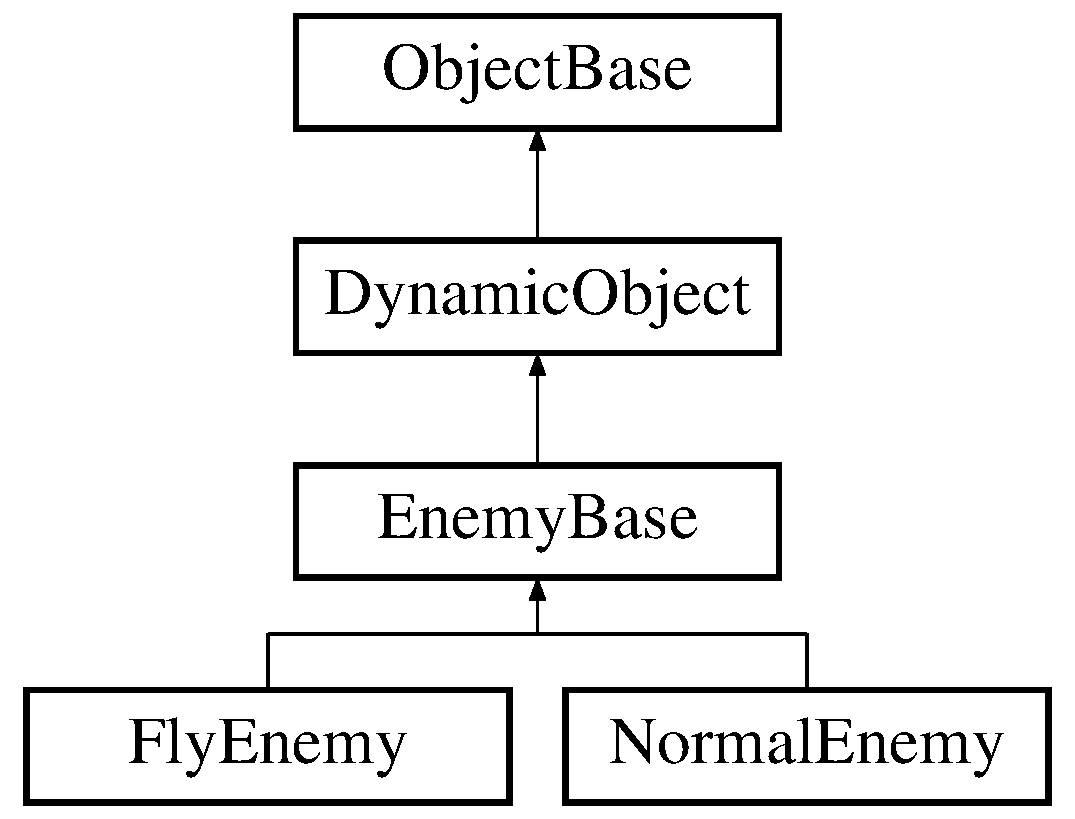
\includegraphics[height=4.000000cm]{class_enemy_base}
\end{center}
\end{figure}
\subsection*{公開メンバ関数}
\begin{DoxyCompactItemize}
\item 
\mbox{\hyperlink{class_enemy_base_abe56e3aa221224c1196fd65f897d5f19}{Enemy\+Base}} (\mbox{\hyperlink{enemy__base_8h_aef73e23ea1cdc9dda520bbb81af707db}{E\+N\+E\+M\+Y\+\_\+\+T\+Y\+PE}} et)
\begin{DoxyCompactList}\small\item\em コンストラクタ \end{DoxyCompactList}\item 
\mbox{\hyperlink{class_enemy_base}{Enemy\+Base}} \& \mbox{\hyperlink{class_enemy_base_ab733c603aedea1306fe42755c784a9db}{operator=}} (const \mbox{\hyperlink{class_enemy_base}{Enemy\+Base}} \&other)
\begin{DoxyCompactList}\small\item\em コピー代入演算子 \end{DoxyCompactList}\end{DoxyCompactItemize}
\subsection*{公開変数類}
\begin{DoxyCompactItemize}
\item 
\mbox{\hyperlink{enemy__base_8h_aef73e23ea1cdc9dda520bbb81af707db}{E\+N\+E\+M\+Y\+\_\+\+T\+Y\+PE}} \mbox{\hyperlink{class_enemy_base_a34ad22e6b0d06b8d63c207c843383eba}{enemy\+\_\+type}}
\end{DoxyCompactItemize}
\subsection*{限定公開メンバ関数}
\begin{DoxyCompactItemize}
\item 
void \mbox{\hyperlink{class_enemy_base_af874ce6fc410fddc7d55ffd7c7bedac8}{Render\+Process}} (bool) final
\begin{DoxyCompactList}\small\item\em 描画 \end{DoxyCompactList}\end{DoxyCompactItemize}
\subsection*{限定公開変数類}
\begin{DoxyCompactItemize}
\item 
\mbox{\hyperlink{class_square_collider}{Square\+Collider}} \mbox{\hyperlink{class_enemy_base_aea91f1e50b8977daa467a3d9fe5f0ef9}{collider}}
\item 
bool \mbox{\hyperlink{class_enemy_base_a0ea15efab9eed801fb676b9276c8e9c9}{destroy\+\_\+flg}} = false
\end{DoxyCompactItemize}


\subsection{詳解}
エネミーのスーパークラス 

\subsection{構築子と解体子}
\mbox{\Hypertarget{class_enemy_base_abe56e3aa221224c1196fd65f897d5f19}\label{class_enemy_base_abe56e3aa221224c1196fd65f897d5f19}} 
\index{Enemy\+Base@{Enemy\+Base}!Enemy\+Base@{Enemy\+Base}}
\index{Enemy\+Base@{Enemy\+Base}!Enemy\+Base@{Enemy\+Base}}
\subsubsection{\texorpdfstring{Enemy\+Base()}{EnemyBase()}}
{\footnotesize\ttfamily Enemy\+Base\+::\+Enemy\+Base (\begin{DoxyParamCaption}\item[{\mbox{\hyperlink{enemy__base_8h_aef73e23ea1cdc9dda520bbb81af707db}{E\+N\+E\+M\+Y\+\_\+\+T\+Y\+PE}}}]{et }\end{DoxyParamCaption})\hspace{0.3cm}{\ttfamily [inline]}}



コンストラクタ 


\begin{DoxyParams}{引数}
{\em et} & 敵のタイプ \\
\hline
\end{DoxyParams}


\subsection{関数詳解}
\mbox{\Hypertarget{class_enemy_base_ab733c603aedea1306fe42755c784a9db}\label{class_enemy_base_ab733c603aedea1306fe42755c784a9db}} 
\index{Enemy\+Base@{Enemy\+Base}!operator=@{operator=}}
\index{operator=@{operator=}!Enemy\+Base@{Enemy\+Base}}
\subsubsection{\texorpdfstring{operator=()}{operator=()}}
{\footnotesize\ttfamily \mbox{\hyperlink{class_enemy_base}{Enemy\+Base}}\& Enemy\+Base\+::operator= (\begin{DoxyParamCaption}\item[{const \mbox{\hyperlink{class_enemy_base}{Enemy\+Base}} \&}]{other }\end{DoxyParamCaption})\hspace{0.3cm}{\ttfamily [inline]}}



コピー代入演算子 

\mbox{\Hypertarget{class_enemy_base_af874ce6fc410fddc7d55ffd7c7bedac8}\label{class_enemy_base_af874ce6fc410fddc7d55ffd7c7bedac8}} 
\index{Enemy\+Base@{Enemy\+Base}!Render\+Process@{Render\+Process}}
\index{Render\+Process@{Render\+Process}!Enemy\+Base@{Enemy\+Base}}
\subsubsection{\texorpdfstring{Render\+Process()}{RenderProcess()}}
{\footnotesize\ttfamily void Enemy\+Base\+::\+Render\+Process (\begin{DoxyParamCaption}\item[{bool}]{camera\+\_\+affected }\end{DoxyParamCaption})\hspace{0.3cm}{\ttfamily [final]}, {\ttfamily [protected]}, {\ttfamily [virtual]}}



描画 


\begin{DoxyParams}{引数}
{\em camera\+\_\+affected} & カメラの位置によって描画する位置を変えるかどうか \\
\hline
\end{DoxyParams}


\mbox{\hyperlink{class_dynamic_object_aa7488e1b4dfd7049447535d93d9d6783}{Dynamic\+Object}}を再実装しています。



\subsection{メンバ詳解}
\mbox{\Hypertarget{class_enemy_base_aea91f1e50b8977daa467a3d9fe5f0ef9}\label{class_enemy_base_aea91f1e50b8977daa467a3d9fe5f0ef9}} 
\index{Enemy\+Base@{Enemy\+Base}!collider@{collider}}
\index{collider@{collider}!Enemy\+Base@{Enemy\+Base}}
\subsubsection{\texorpdfstring{collider}{collider}}
{\footnotesize\ttfamily \mbox{\hyperlink{class_square_collider}{Square\+Collider}} Enemy\+Base\+::collider\hspace{0.3cm}{\ttfamily [protected]}}

\mbox{\Hypertarget{class_enemy_base_a0ea15efab9eed801fb676b9276c8e9c9}\label{class_enemy_base_a0ea15efab9eed801fb676b9276c8e9c9}} 
\index{Enemy\+Base@{Enemy\+Base}!destroy\+\_\+flg@{destroy\+\_\+flg}}
\index{destroy\+\_\+flg@{destroy\+\_\+flg}!Enemy\+Base@{Enemy\+Base}}
\subsubsection{\texorpdfstring{destroy\+\_\+flg}{destroy\_flg}}
{\footnotesize\ttfamily bool Enemy\+Base\+::destroy\+\_\+flg = false\hspace{0.3cm}{\ttfamily [protected]}}

\mbox{\Hypertarget{class_enemy_base_a34ad22e6b0d06b8d63c207c843383eba}\label{class_enemy_base_a34ad22e6b0d06b8d63c207c843383eba}} 
\index{Enemy\+Base@{Enemy\+Base}!enemy\+\_\+type@{enemy\+\_\+type}}
\index{enemy\+\_\+type@{enemy\+\_\+type}!Enemy\+Base@{Enemy\+Base}}
\subsubsection{\texorpdfstring{enemy\+\_\+type}{enemy\_type}}
{\footnotesize\ttfamily \mbox{\hyperlink{enemy__base_8h_aef73e23ea1cdc9dda520bbb81af707db}{E\+N\+E\+M\+Y\+\_\+\+T\+Y\+PE}} Enemy\+Base\+::enemy\+\_\+type}



このクラス詳解は次のファイルから抽出されました\+:\begin{DoxyCompactItemize}
\item 
C\+:/\+Users/tokir/\+Documents/\+Git\+Hub/\+Weapon\+Merchant\+Adventure/src/src/object/character/enemy/base/\mbox{\hyperlink{enemy__base_8h}{enemy\+\_\+base.\+h}}\item 
C\+:/\+Users/tokir/\+Documents/\+Git\+Hub/\+Weapon\+Merchant\+Adventure/src/src/object/character/enemy/base/\mbox{\hyperlink{enemy__base_8cpp}{enemy\+\_\+base.\+cpp}}\end{DoxyCompactItemize}

\hypertarget{class_fade}{}\section{Fade クラス}
\label{class_fade}\index{Fade@{Fade}}


フェードクラス  




{\ttfamily \#include $<$fade.\+h$>$}

Fade の継承関係図\begin{figure}[H]
\begin{center}
\leavevmode
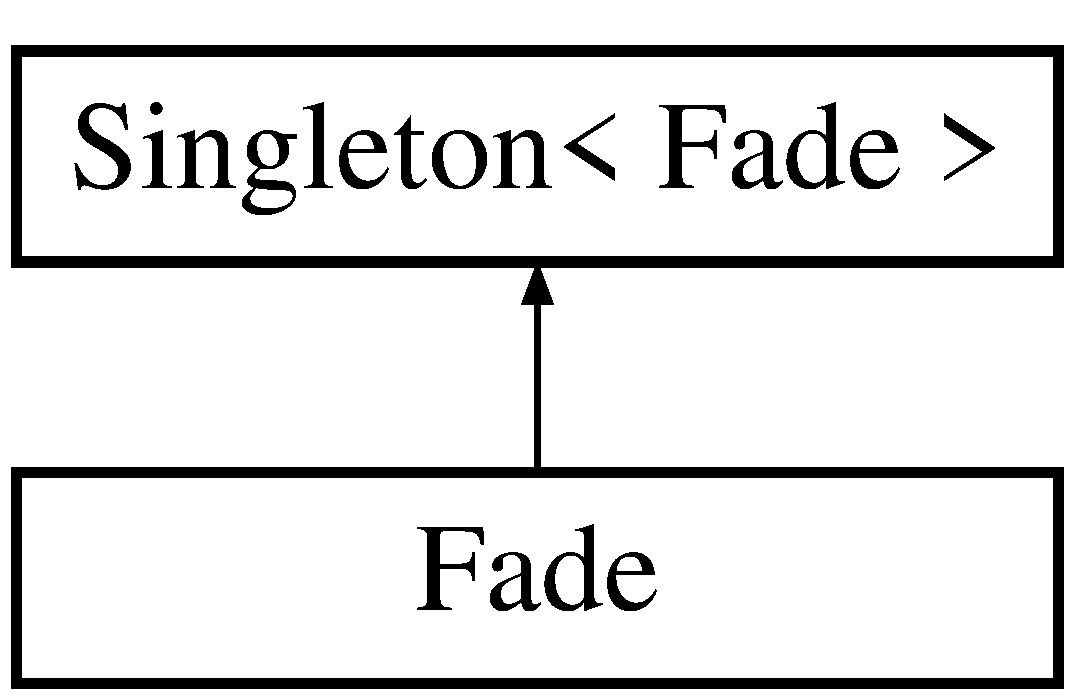
\includegraphics[height=2.000000cm]{class_fade}
\end{center}
\end{figure}
\subsection*{公開メンバ関数}
\begin{DoxyCompactItemize}
\item 
void \mbox{\hyperlink{class_fade_ac2a47819e1390abcae3259bcb42bddf5}{Init}} ()
\begin{DoxyCompactList}\small\item\em 初期化 \end{DoxyCompactList}\item 
bool \mbox{\hyperlink{class_fade_aaf97d1ac502c86612a97fde0e2fbf308}{Update}} (const bool)
\begin{DoxyCompactList}\small\item\em 更新 \end{DoxyCompactList}\item 
void \mbox{\hyperlink{class_fade_abfe024be1a10d4849582adf58fe6682a}{Render}} ()
\begin{DoxyCompactList}\small\item\em 描画 \end{DoxyCompactList}\item 
void \mbox{\hyperlink{class_fade_afd5cce157c2876a800ea59b2648547c2}{Destroy}} ()
\begin{DoxyCompactList}\small\item\em 破棄 \end{DoxyCompactList}\end{DoxyCompactItemize}
\subsection*{その他の継承メンバ}


\subsection{詳解}
フェードクラス 

\subsection{関数詳解}
\mbox{\Hypertarget{class_fade_afd5cce157c2876a800ea59b2648547c2}\label{class_fade_afd5cce157c2876a800ea59b2648547c2}} 
\index{Fade@{Fade}!Destroy@{Destroy}}
\index{Destroy@{Destroy}!Fade@{Fade}}
\subsubsection{\texorpdfstring{Destroy()}{Destroy()}}
{\footnotesize\ttfamily void Fade\+::\+Destroy (\begin{DoxyParamCaption}{ }\end{DoxyParamCaption})}



破棄 

\mbox{\Hypertarget{class_fade_ac2a47819e1390abcae3259bcb42bddf5}\label{class_fade_ac2a47819e1390abcae3259bcb42bddf5}} 
\index{Fade@{Fade}!Init@{Init}}
\index{Init@{Init}!Fade@{Fade}}
\subsubsection{\texorpdfstring{Init()}{Init()}}
{\footnotesize\ttfamily void Fade\+::\+Init (\begin{DoxyParamCaption}{ }\end{DoxyParamCaption})}



初期化 

\mbox{\Hypertarget{class_fade_abfe024be1a10d4849582adf58fe6682a}\label{class_fade_abfe024be1a10d4849582adf58fe6682a}} 
\index{Fade@{Fade}!Render@{Render}}
\index{Render@{Render}!Fade@{Fade}}
\subsubsection{\texorpdfstring{Render()}{Render()}}
{\footnotesize\ttfamily void Fade\+::\+Render (\begin{DoxyParamCaption}{ }\end{DoxyParamCaption})}



描画 

\mbox{\Hypertarget{class_fade_aaf97d1ac502c86612a97fde0e2fbf308}\label{class_fade_aaf97d1ac502c86612a97fde0e2fbf308}} 
\index{Fade@{Fade}!Update@{Update}}
\index{Update@{Update}!Fade@{Fade}}
\subsubsection{\texorpdfstring{Update()}{Update()}}
{\footnotesize\ttfamily bool Fade\+::\+Update (\begin{DoxyParamCaption}\item[{const bool}]{fade\+\_\+in }\end{DoxyParamCaption})}



更新 


\begin{DoxyParams}{引数}
{\em fade\+\_\+in} & フェードインかどうか \\
\hline
\end{DoxyParams}
\begin{DoxyReturn}{戻り値}
bool フェードインかアウトが終わったらtrue 
\end{DoxyReturn}


このクラス詳解は次のファイルから抽出されました\+:\begin{DoxyCompactItemize}
\item 
C\+:/\+Users/tokir/\+Documents/\+Git\+Hub/\+Weapon\+Merchant\+Adventure/src/scene/fade/\mbox{\hyperlink{fade_8h}{fade.\+h}}\item 
C\+:/\+Users/tokir/\+Documents/\+Git\+Hub/\+Weapon\+Merchant\+Adventure/src/scene/fade/\mbox{\hyperlink{fade_8cpp}{fade.\+cpp}}\end{DoxyCompactItemize}

\hypertarget{class_fly_enemy}{}\section{Fly\+Enemy クラス}
\label{class_fly_enemy}\index{Fly\+Enemy@{Fly\+Enemy}}


飛ぶエネミークラス  




{\ttfamily \#include $<$fly\+\_\+enemy.\+h$>$}

Fly\+Enemy の継承関係図\begin{figure}[H]
\begin{center}
\leavevmode
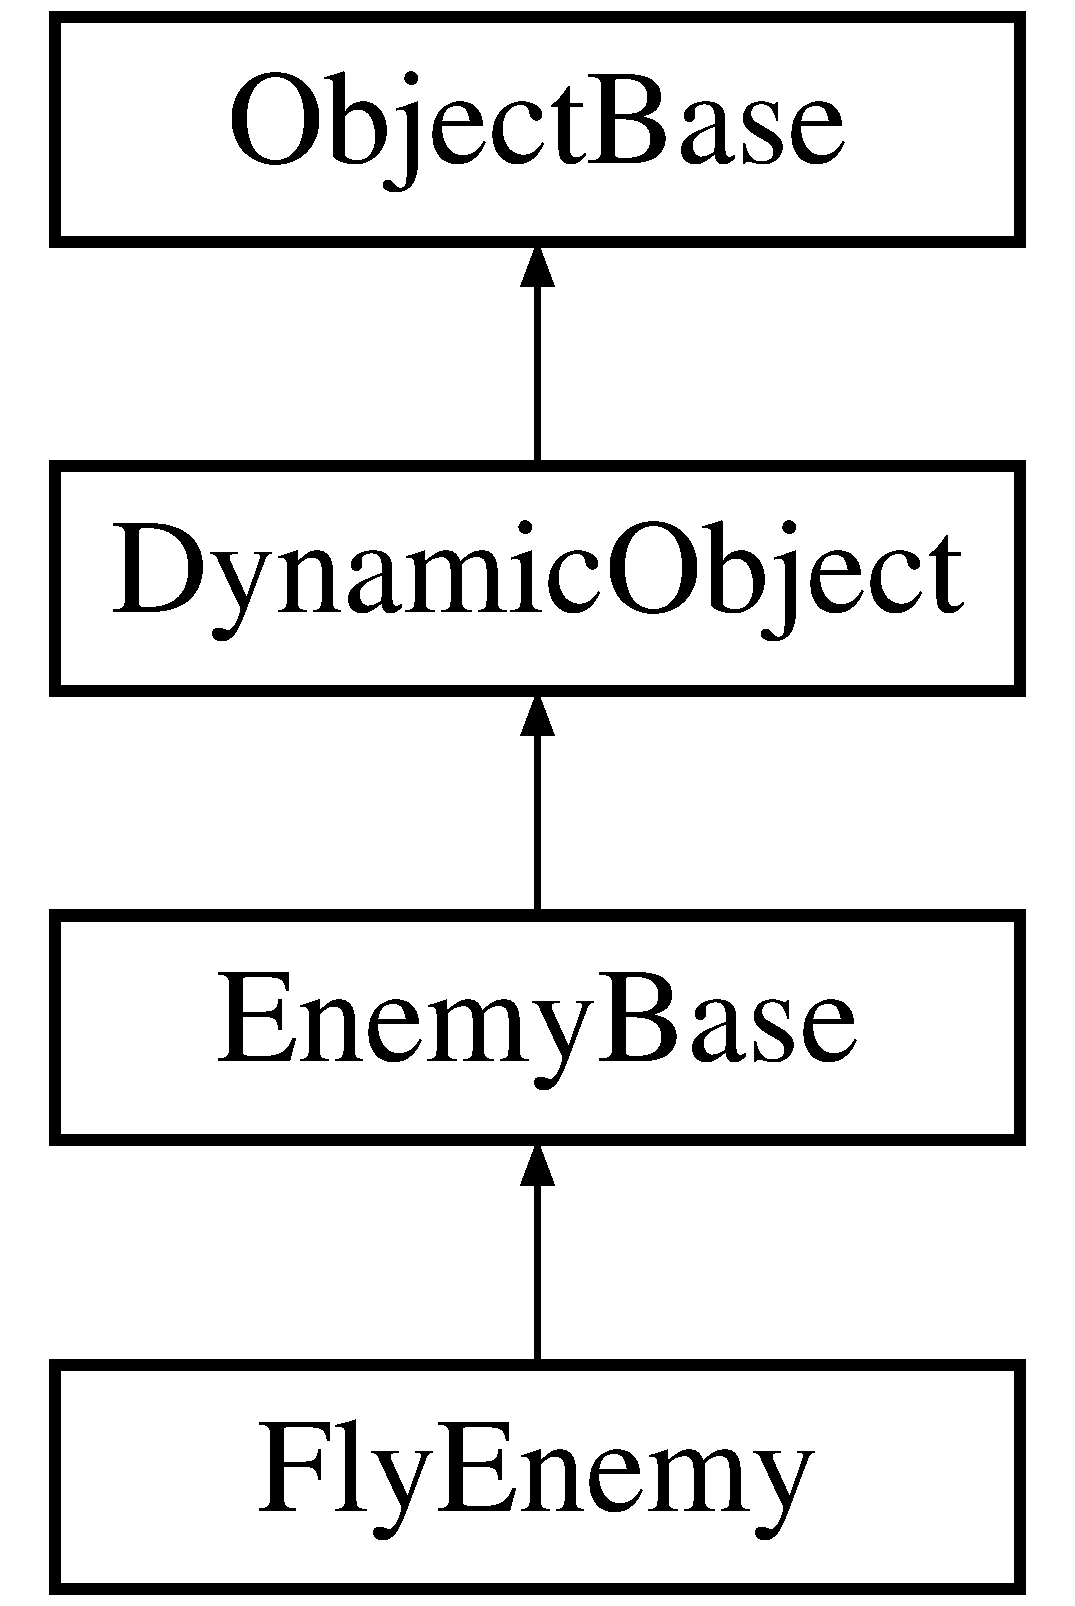
\includegraphics[height=4.000000cm]{class_fly_enemy}
\end{center}
\end{figure}
\subsection*{公開メンバ関数}
\begin{DoxyCompactItemize}
\item 
\mbox{\hyperlink{class_fly_enemy_a92bb66e1f877440afab15a36ffebd74d}{Fly\+Enemy}} ()
\begin{DoxyCompactList}\small\item\em コンストラクタ \end{DoxyCompactList}\item 
\mbox{\hyperlink{class_fly_enemy_af206898a5e1b59cc7bba2e4c13b72384}{Fly\+Enemy}} (const \mbox{\hyperlink{class_fly_enemy}{Fly\+Enemy}} \&ne)
\begin{DoxyCompactList}\small\item\em コピーコンストラクタ \end{DoxyCompactList}\item 
\mbox{\hyperlink{class_fly_enemy_ad32ad41958e55f3028b0beb068813bc1}{Fly\+Enemy}} (\mbox{\hyperlink{class_fly_enemy}{Fly\+Enemy}} \&\&ne)
\begin{DoxyCompactList}\small\item\em ムーブコンストラクタ \end{DoxyCompactList}\item 
\mbox{\hyperlink{class_fly_enemy}{Fly\+Enemy}} \& \mbox{\hyperlink{class_fly_enemy_a6cc3f3701b503020620c02667705fd23}{operator=}} (const \mbox{\hyperlink{class_fly_enemy}{Fly\+Enemy}} \&other)
\begin{DoxyCompactList}\small\item\em コピー代入演算子 \end{DoxyCompactList}\item 
void \mbox{\hyperlink{class_fly_enemy_adaabf7ce270104e30df29bfa464d72ce}{Collision}} (\mbox{\hyperlink{class_object_base}{Object\+Base}} $\ast$, \mbox{\hyperlink{common_8h_afb0c5e21d4133ff4f200992c0b534e1b}{V\+E\+C2}}) final
\begin{DoxyCompactList}\small\item\em 当たったときに実行する関数 \end{DoxyCompactList}\item 
void \mbox{\hyperlink{class_fly_enemy_af7ce5137e8eb2e8cc6654fbbdbc714cd}{Destroy}} () final
\begin{DoxyCompactList}\small\item\em 破棄 \end{DoxyCompactList}\item 
\mbox{\hyperlink{class_fly_enemy_ae4345f89a659b559c08d0bb879db7158}{$\sim$\+Fly\+Enemy}} ()
\begin{DoxyCompactList}\small\item\em デストラクタ \end{DoxyCompactList}\item 
void \mbox{\hyperlink{class_fly_enemy_a137e5a5f2adb7eacd282bbf662242cb3}{Set\+Move}} (const \mbox{\hyperlink{common_8h_afb0c5e21d4133ff4f200992c0b534e1b}{V\+E\+C2}} \&range, float time)
\begin{DoxyCompactList}\small\item\em 移動範囲を決める \end{DoxyCompactList}\end{DoxyCompactItemize}
\subsection*{限定公開メンバ関数}
\begin{DoxyCompactItemize}
\item 
void \mbox{\hyperlink{class_fly_enemy_afe4ddbf7089952146443f4ca71f55b13}{Init\+Process}} () final
\begin{DoxyCompactList}\small\item\em 初期化 \end{DoxyCompactList}\item 
void \mbox{\hyperlink{class_fly_enemy_a5122c8fea26ebbd0390acfd6e41931ff}{Update\+Process}} () final
\begin{DoxyCompactList}\small\item\em 更新 \end{DoxyCompactList}\end{DoxyCompactItemize}
\subsection*{その他の継承メンバ}


\subsection{詳解}
飛ぶエネミークラス 

\subsection{構築子と解体子}
\mbox{\Hypertarget{class_fly_enemy_a92bb66e1f877440afab15a36ffebd74d}\label{class_fly_enemy_a92bb66e1f877440afab15a36ffebd74d}} 
\index{Fly\+Enemy@{Fly\+Enemy}!Fly\+Enemy@{Fly\+Enemy}}
\index{Fly\+Enemy@{Fly\+Enemy}!Fly\+Enemy@{Fly\+Enemy}}
\subsubsection{\texorpdfstring{Fly\+Enemy()}{FlyEnemy()}\hspace{0.1cm}{\footnotesize\ttfamily [1/3]}}
{\footnotesize\ttfamily Fly\+Enemy\+::\+Fly\+Enemy (\begin{DoxyParamCaption}{ }\end{DoxyParamCaption})\hspace{0.3cm}{\ttfamily [inline]}}



コンストラクタ 

\mbox{\Hypertarget{class_fly_enemy_af206898a5e1b59cc7bba2e4c13b72384}\label{class_fly_enemy_af206898a5e1b59cc7bba2e4c13b72384}} 
\index{Fly\+Enemy@{Fly\+Enemy}!Fly\+Enemy@{Fly\+Enemy}}
\index{Fly\+Enemy@{Fly\+Enemy}!Fly\+Enemy@{Fly\+Enemy}}
\subsubsection{\texorpdfstring{Fly\+Enemy()}{FlyEnemy()}\hspace{0.1cm}{\footnotesize\ttfamily [2/3]}}
{\footnotesize\ttfamily Fly\+Enemy\+::\+Fly\+Enemy (\begin{DoxyParamCaption}\item[{const \mbox{\hyperlink{class_fly_enemy}{Fly\+Enemy}} \&}]{ne }\end{DoxyParamCaption})\hspace{0.3cm}{\ttfamily [inline]}}



コピーコンストラクタ 

\mbox{\Hypertarget{class_fly_enemy_ad32ad41958e55f3028b0beb068813bc1}\label{class_fly_enemy_ad32ad41958e55f3028b0beb068813bc1}} 
\index{Fly\+Enemy@{Fly\+Enemy}!Fly\+Enemy@{Fly\+Enemy}}
\index{Fly\+Enemy@{Fly\+Enemy}!Fly\+Enemy@{Fly\+Enemy}}
\subsubsection{\texorpdfstring{Fly\+Enemy()}{FlyEnemy()}\hspace{0.1cm}{\footnotesize\ttfamily [3/3]}}
{\footnotesize\ttfamily Fly\+Enemy\+::\+Fly\+Enemy (\begin{DoxyParamCaption}\item[{\mbox{\hyperlink{class_fly_enemy}{Fly\+Enemy}} \&\&}]{ne }\end{DoxyParamCaption})\hspace{0.3cm}{\ttfamily [inline]}}



ムーブコンストラクタ 

\mbox{\Hypertarget{class_fly_enemy_ae4345f89a659b559c08d0bb879db7158}\label{class_fly_enemy_ae4345f89a659b559c08d0bb879db7158}} 
\index{Fly\+Enemy@{Fly\+Enemy}!````~Fly\+Enemy@{$\sim$\+Fly\+Enemy}}
\index{````~Fly\+Enemy@{$\sim$\+Fly\+Enemy}!Fly\+Enemy@{Fly\+Enemy}}
\subsubsection{\texorpdfstring{$\sim$\+Fly\+Enemy()}{~FlyEnemy()}}
{\footnotesize\ttfamily Fly\+Enemy\+::$\sim$\+Fly\+Enemy (\begin{DoxyParamCaption}{ }\end{DoxyParamCaption})\hspace{0.3cm}{\ttfamily [inline]}}



デストラクタ 



\subsection{関数詳解}
\mbox{\Hypertarget{class_fly_enemy_adaabf7ce270104e30df29bfa464d72ce}\label{class_fly_enemy_adaabf7ce270104e30df29bfa464d72ce}} 
\index{Fly\+Enemy@{Fly\+Enemy}!Collision@{Collision}}
\index{Collision@{Collision}!Fly\+Enemy@{Fly\+Enemy}}
\subsubsection{\texorpdfstring{Collision()}{Collision()}}
{\footnotesize\ttfamily void Fly\+Enemy\+::\+Collision (\begin{DoxyParamCaption}\item[{\mbox{\hyperlink{class_object_base}{Object\+Base}} $\ast$}]{obj,  }\item[{\mbox{\hyperlink{common_8h_afb0c5e21d4133ff4f200992c0b534e1b}{V\+E\+C2}}}]{ }\end{DoxyParamCaption})\hspace{0.3cm}{\ttfamily [final]}, {\ttfamily [virtual]}}



当たったときに実行する関数 


\begin{DoxyParams}{引数}
{\em obj} & 当たった相手のオブジェクト \\
\hline
\end{DoxyParams}


\mbox{\hyperlink{class_object_base_ad772d7a42f5e46c39481f5db22ee8193}{Object\+Base}}を再実装しています。

\mbox{\Hypertarget{class_fly_enemy_af7ce5137e8eb2e8cc6654fbbdbc714cd}\label{class_fly_enemy_af7ce5137e8eb2e8cc6654fbbdbc714cd}} 
\index{Fly\+Enemy@{Fly\+Enemy}!Destroy@{Destroy}}
\index{Destroy@{Destroy}!Fly\+Enemy@{Fly\+Enemy}}
\subsubsection{\texorpdfstring{Destroy()}{Destroy()}}
{\footnotesize\ttfamily void Fly\+Enemy\+::\+Destroy (\begin{DoxyParamCaption}{ }\end{DoxyParamCaption})\hspace{0.3cm}{\ttfamily [final]}, {\ttfamily [virtual]}}



破棄 



\mbox{\hyperlink{class_object_base_a7fa4c548153c3af20f89673ffea809af}{Object\+Base}}を実装しています。

\mbox{\Hypertarget{class_fly_enemy_afe4ddbf7089952146443f4ca71f55b13}\label{class_fly_enemy_afe4ddbf7089952146443f4ca71f55b13}} 
\index{Fly\+Enemy@{Fly\+Enemy}!Init\+Process@{Init\+Process}}
\index{Init\+Process@{Init\+Process}!Fly\+Enemy@{Fly\+Enemy}}
\subsubsection{\texorpdfstring{Init\+Process()}{InitProcess()}}
{\footnotesize\ttfamily void Fly\+Enemy\+::\+Init\+Process (\begin{DoxyParamCaption}{ }\end{DoxyParamCaption})\hspace{0.3cm}{\ttfamily [final]}, {\ttfamily [protected]}, {\ttfamily [virtual]}}



初期化 



\mbox{\hyperlink{class_object_base_af133f36f2bca1dcfd962e2cfac61ab51}{Object\+Base}}を実装しています。

\mbox{\Hypertarget{class_fly_enemy_a6cc3f3701b503020620c02667705fd23}\label{class_fly_enemy_a6cc3f3701b503020620c02667705fd23}} 
\index{Fly\+Enemy@{Fly\+Enemy}!operator=@{operator=}}
\index{operator=@{operator=}!Fly\+Enemy@{Fly\+Enemy}}
\subsubsection{\texorpdfstring{operator=()}{operator=()}}
{\footnotesize\ttfamily \mbox{\hyperlink{class_fly_enemy}{Fly\+Enemy}}\& Fly\+Enemy\+::operator= (\begin{DoxyParamCaption}\item[{const \mbox{\hyperlink{class_fly_enemy}{Fly\+Enemy}} \&}]{other }\end{DoxyParamCaption})\hspace{0.3cm}{\ttfamily [inline]}}



コピー代入演算子 

\mbox{\Hypertarget{class_fly_enemy_a137e5a5f2adb7eacd282bbf662242cb3}\label{class_fly_enemy_a137e5a5f2adb7eacd282bbf662242cb3}} 
\index{Fly\+Enemy@{Fly\+Enemy}!Set\+Move@{Set\+Move}}
\index{Set\+Move@{Set\+Move}!Fly\+Enemy@{Fly\+Enemy}}
\subsubsection{\texorpdfstring{Set\+Move()}{SetMove()}}
{\footnotesize\ttfamily void Fly\+Enemy\+::\+Set\+Move (\begin{DoxyParamCaption}\item[{const \mbox{\hyperlink{common_8h_afb0c5e21d4133ff4f200992c0b534e1b}{V\+E\+C2}} \&}]{range,  }\item[{float}]{time }\end{DoxyParamCaption})\hspace{0.3cm}{\ttfamily [inline]}}



移動範囲を決める 


\begin{DoxyParams}{引数}
{\em range} & 現在の位置からどのくらい移動するか \\
\hline
{\em time} & どのくらいの時間をかけて行き来するか \\
\hline
\end{DoxyParams}
\mbox{\Hypertarget{class_fly_enemy_a5122c8fea26ebbd0390acfd6e41931ff}\label{class_fly_enemy_a5122c8fea26ebbd0390acfd6e41931ff}} 
\index{Fly\+Enemy@{Fly\+Enemy}!Update\+Process@{Update\+Process}}
\index{Update\+Process@{Update\+Process}!Fly\+Enemy@{Fly\+Enemy}}
\subsubsection{\texorpdfstring{Update\+Process()}{UpdateProcess()}}
{\footnotesize\ttfamily void Fly\+Enemy\+::\+Update\+Process (\begin{DoxyParamCaption}{ }\end{DoxyParamCaption})\hspace{0.3cm}{\ttfamily [final]}, {\ttfamily [protected]}, {\ttfamily [virtual]}}



更新 



\mbox{\hyperlink{class_object_base_a8b5b72b363a419767efde0b0e692ea95}{Object\+Base}}を実装しています。



このクラス詳解は次のファイルから抽出されました\+:\begin{DoxyCompactItemize}
\item 
C\+:/\+Users/tokir/\+Documents/\+Git\+Hub/\+Weapon\+Merchant\+Adventure/src/object/character/enemy/fly/\mbox{\hyperlink{fly__enemy_8h}{fly\+\_\+enemy.\+h}}\item 
C\+:/\+Users/tokir/\+Documents/\+Git\+Hub/\+Weapon\+Merchant\+Adventure/src/object/character/enemy/fly/\mbox{\hyperlink{fly__enemy_8cpp}{fly\+\_\+enemy.\+cpp}}\end{DoxyCompactItemize}

\hypertarget{class_font}{}\section{Font クラス}
\label{class_font}\index{Font@{Font}}


フォントクラス  




{\ttfamily \#include $<$font.\+h$>$}

\subsection*{公開メンバ関数}
\begin{DoxyCompactItemize}
\item 
\mbox{\hyperlink{class_font_a2af6642bc26eebff029c74d7827f5ee5}{Font}} ()=delete
\item 
\mbox{\hyperlink{class_font_aa07b69b4e229b2e9efdf0ac49e7a2af1}{Font}} (const \mbox{\hyperlink{class_transform}{Transform}} \&)
\begin{DoxyCompactList}\small\item\em コンストラクタ \end{DoxyCompactList}\item 
void \mbox{\hyperlink{class_font_a35fd445e07010a3ad2c74c93dfa33f66}{Init}} (W\+C\+H\+AR $\ast$\+\_\+text, float r=1, float g=1, float b=1, float a=1)
\begin{DoxyCompactList}\small\item\em 初期化 \end{DoxyCompactList}\item 
void \mbox{\hyperlink{class_font_ad0e36f0066cc8724b6cf6833a15aedbc}{Render}} ()
\begin{DoxyCompactList}\small\item\em 描画 \end{DoxyCompactList}\item 
void \mbox{\hyperlink{class_font_a2c862120802e9aac650a96f7b4e29081}{Set\+Text}} (W\+C\+H\+AR $\ast$\+\_\+text)
\begin{DoxyCompactList}\small\item\em 文字列のセット \end{DoxyCompactList}\item 
W\+C\+H\+AR $\ast$ \mbox{\hyperlink{class_font_a47be569e73a4ba819bf4370463cf929b}{Get\+Text}} ()
\begin{DoxyCompactList}\small\item\em テキストを取得する \end{DoxyCompactList}\end{DoxyCompactItemize}


\subsection{詳解}
フォントクラス 

\subsection{構築子と解体子}
\mbox{\Hypertarget{class_font_a2af6642bc26eebff029c74d7827f5ee5}\label{class_font_a2af6642bc26eebff029c74d7827f5ee5}} 
\index{Font@{Font}!Font@{Font}}
\index{Font@{Font}!Font@{Font}}
\subsubsection{\texorpdfstring{Font()}{Font()}\hspace{0.1cm}{\footnotesize\ttfamily [1/2]}}
{\footnotesize\ttfamily Font\+::\+Font (\begin{DoxyParamCaption}{ }\end{DoxyParamCaption})\hspace{0.3cm}{\ttfamily [delete]}}

\mbox{\Hypertarget{class_font_aa07b69b4e229b2e9efdf0ac49e7a2af1}\label{class_font_aa07b69b4e229b2e9efdf0ac49e7a2af1}} 
\index{Font@{Font}!Font@{Font}}
\index{Font@{Font}!Font@{Font}}
\subsubsection{\texorpdfstring{Font()}{Font()}\hspace{0.1cm}{\footnotesize\ttfamily [2/2]}}
{\footnotesize\ttfamily Font\+::\+Font (\begin{DoxyParamCaption}\item[{const \mbox{\hyperlink{class_transform}{Transform}} \&}]{t }\end{DoxyParamCaption})}



コンストラクタ 


\begin{DoxyParams}{引数}
{\em t} & Transformの参照 \\
\hline
\end{DoxyParams}


\subsection{関数詳解}
\mbox{\Hypertarget{class_font_a47be569e73a4ba819bf4370463cf929b}\label{class_font_a47be569e73a4ba819bf4370463cf929b}} 
\index{Font@{Font}!Get\+Text@{Get\+Text}}
\index{Get\+Text@{Get\+Text}!Font@{Font}}
\subsubsection{\texorpdfstring{Get\+Text()}{GetText()}}
{\footnotesize\ttfamily W\+C\+H\+AR$\ast$ Font\+::\+Get\+Text (\begin{DoxyParamCaption}{ }\end{DoxyParamCaption})\hspace{0.3cm}{\ttfamily [inline]}}



テキストを取得する 

\begin{DoxyReturn}{戻り値}
W\+C\+H\+A\+R$\ast$ テキスト 
\end{DoxyReturn}
\mbox{\Hypertarget{class_font_a35fd445e07010a3ad2c74c93dfa33f66}\label{class_font_a35fd445e07010a3ad2c74c93dfa33f66}} 
\index{Font@{Font}!Init@{Init}}
\index{Init@{Init}!Font@{Font}}
\subsubsection{\texorpdfstring{Init()}{Init()}}
{\footnotesize\ttfamily void Font\+::\+Init (\begin{DoxyParamCaption}\item[{W\+C\+H\+AR $\ast$}]{\+\_\+text,  }\item[{float}]{r = {\ttfamily 1},  }\item[{float}]{g = {\ttfamily 1},  }\item[{float}]{b = {\ttfamily 1},  }\item[{float}]{a = {\ttfamily 1} }\end{DoxyParamCaption})}



初期化 


\begin{DoxyParams}{引数}
{\em \+\_\+text} & テキスト \\
\hline
{\em r,g,b,a} & 色 \\
\hline
\end{DoxyParams}
\mbox{\Hypertarget{class_font_ad0e36f0066cc8724b6cf6833a15aedbc}\label{class_font_ad0e36f0066cc8724b6cf6833a15aedbc}} 
\index{Font@{Font}!Render@{Render}}
\index{Render@{Render}!Font@{Font}}
\subsubsection{\texorpdfstring{Render()}{Render()}}
{\footnotesize\ttfamily void Font\+::\+Render (\begin{DoxyParamCaption}{ }\end{DoxyParamCaption})}



描画 

\mbox{\Hypertarget{class_font_a2c862120802e9aac650a96f7b4e29081}\label{class_font_a2c862120802e9aac650a96f7b4e29081}} 
\index{Font@{Font}!Set\+Text@{Set\+Text}}
\index{Set\+Text@{Set\+Text}!Font@{Font}}
\subsubsection{\texorpdfstring{Set\+Text()}{SetText()}}
{\footnotesize\ttfamily void Font\+::\+Set\+Text (\begin{DoxyParamCaption}\item[{W\+C\+H\+AR $\ast$}]{\+\_\+text }\end{DoxyParamCaption})\hspace{0.3cm}{\ttfamily [inline]}}



文字列のセット 


\begin{DoxyParams}{引数}
{\em \+\_\+text} & セットする文字列 \\
\hline
\end{DoxyParams}


このクラス詳解は次のファイルから抽出されました\+:\begin{DoxyCompactItemize}
\item 
C\+:/\+Users/tokir/\+Documents/\+Git\+Hub/\+Weapon\+Merchant\+Adventure/src/rendering/font/\mbox{\hyperlink{font_8h}{font.\+h}}\item 
C\+:/\+Users/tokir/\+Documents/\+Git\+Hub/\+Weapon\+Merchant\+Adventure/src/rendering/font/\mbox{\hyperlink{font_8cpp}{font.\+cpp}}\end{DoxyCompactItemize}

\hypertarget{struct_font_color}{}\section{Font\+Color 構造体}
\label{struct_font_color}\index{Font\+Color@{Font\+Color}}


フォント用の色構造体  




{\ttfamily \#include $<$font.\+h$>$}

\subsection*{公開変数類}
\begin{DoxyCompactItemize}
\item 
float \mbox{\hyperlink{struct_font_color_a194c6908e2594b30387e7e127e340f87}{r}}
\item 
float \mbox{\hyperlink{struct_font_color_aee91e6024a40a2bc4a21cc427c9102a6}{g}}
\item 
float \mbox{\hyperlink{struct_font_color_af282546f7dc30a812f5f174f7bf33098}{b}}
\item 
float \mbox{\hyperlink{struct_font_color_aa093d6bd66be078e43a00e1c9048403b}{a}}
\end{DoxyCompactItemize}


\subsection{詳解}
フォント用の色構造体 

\subsection{メンバ詳解}
\mbox{\Hypertarget{struct_font_color_aa093d6bd66be078e43a00e1c9048403b}\label{struct_font_color_aa093d6bd66be078e43a00e1c9048403b}} 
\index{Font\+Color@{Font\+Color}!a@{a}}
\index{a@{a}!Font\+Color@{Font\+Color}}
\subsubsection{\texorpdfstring{a}{a}}
{\footnotesize\ttfamily float Font\+Color\+::a}

\mbox{\Hypertarget{struct_font_color_af282546f7dc30a812f5f174f7bf33098}\label{struct_font_color_af282546f7dc30a812f5f174f7bf33098}} 
\index{Font\+Color@{Font\+Color}!b@{b}}
\index{b@{b}!Font\+Color@{Font\+Color}}
\subsubsection{\texorpdfstring{b}{b}}
{\footnotesize\ttfamily float Font\+Color\+::b}

\mbox{\Hypertarget{struct_font_color_aee91e6024a40a2bc4a21cc427c9102a6}\label{struct_font_color_aee91e6024a40a2bc4a21cc427c9102a6}} 
\index{Font\+Color@{Font\+Color}!g@{g}}
\index{g@{g}!Font\+Color@{Font\+Color}}
\subsubsection{\texorpdfstring{g}{g}}
{\footnotesize\ttfamily float Font\+Color\+::g}

\mbox{\Hypertarget{struct_font_color_a194c6908e2594b30387e7e127e340f87}\label{struct_font_color_a194c6908e2594b30387e7e127e340f87}} 
\index{Font\+Color@{Font\+Color}!r@{r}}
\index{r@{r}!Font\+Color@{Font\+Color}}
\subsubsection{\texorpdfstring{r}{r}}
{\footnotesize\ttfamily float Font\+Color\+::r}



この構造体詳解は次のファイルから抽出されました\+:\begin{DoxyCompactItemize}
\item 
C\+:/\+Users/tokir/\+Documents/\+Git\+Hub/\+Weapon\+Merchant\+Adventure/src/rendering/font/\mbox{\hyperlink{font_8h}{font.\+h}}\end{DoxyCompactItemize}

\hypertarget{class_font_manager}{}\section{Font\+Manager クラス}
\label{class_font_manager}\index{Font\+Manager@{Font\+Manager}}


フォントを管理するクラス  




{\ttfamily \#include $<$font\+\_\+manager.\+h$>$}

Font\+Manager の継承関係図\begin{figure}[H]
\begin{center}
\leavevmode
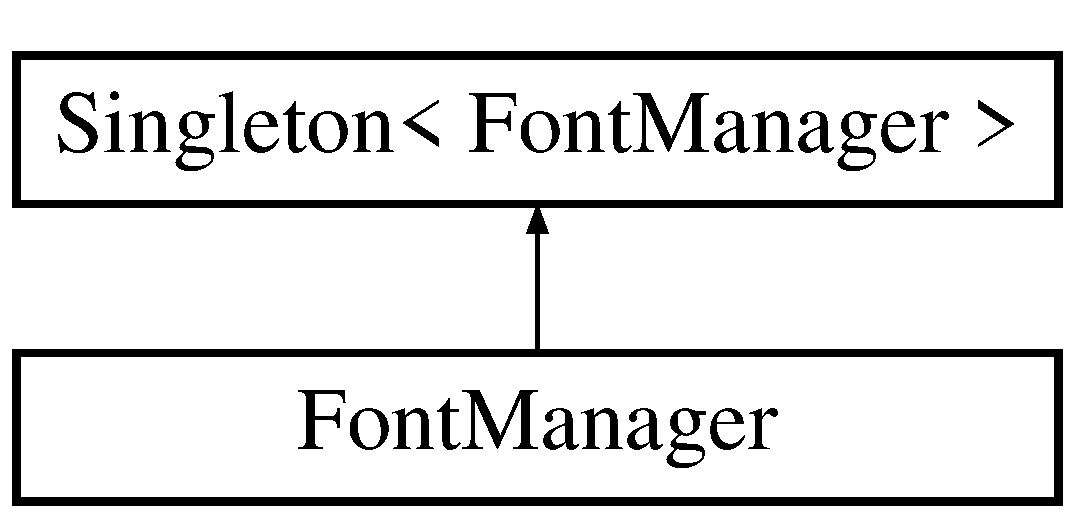
\includegraphics[height=2.000000cm]{class_font_manager}
\end{center}
\end{figure}
\subsection*{公開メンバ関数}
\begin{DoxyCompactItemize}
\item 
void \mbox{\hyperlink{class_font_manager_acabba97ebae69b7b92d2ea4a2e9216e4}{Init}} (I\+D3\+D11\+Device $\ast$, W\+C\+H\+AR $\ast$)
\begin{DoxyCompactList}\small\item\em 初期化 \end{DoxyCompactList}\item 
\mbox{\hyperlink{class_font_manager_aa190bb023b4cf2ad28e24c69ef57f380}{$\sim$\+Font\+Manager}} ()
\begin{DoxyCompactList}\small\item\em デストラクタ \end{DoxyCompactList}\item 
std\+::unique\+\_\+ptr$<$ Direct\+X\+::\+Sprite\+Font $>$ \& \mbox{\hyperlink{class_font_manager_a612a8922fc977b07959406468dec922f}{Get\+Sprite\+Font}} ()
\begin{DoxyCompactList}\small\item\em Sprite\+Fontのゲッタ \end{DoxyCompactList}\end{DoxyCompactItemize}
\subsection*{その他の継承メンバ}


\subsection{詳解}
フォントを管理するクラス 

\subsection{構築子と解体子}
\mbox{\Hypertarget{class_font_manager_aa190bb023b4cf2ad28e24c69ef57f380}\label{class_font_manager_aa190bb023b4cf2ad28e24c69ef57f380}} 
\index{Font\+Manager@{Font\+Manager}!````~Font\+Manager@{$\sim$\+Font\+Manager}}
\index{````~Font\+Manager@{$\sim$\+Font\+Manager}!Font\+Manager@{Font\+Manager}}
\subsubsection{\texorpdfstring{$\sim$\+Font\+Manager()}{~FontManager()}}
{\footnotesize\ttfamily Font\+Manager\+::$\sim$\+Font\+Manager (\begin{DoxyParamCaption}{ }\end{DoxyParamCaption})}



デストラクタ 



\subsection{関数詳解}
\mbox{\Hypertarget{class_font_manager_a612a8922fc977b07959406468dec922f}\label{class_font_manager_a612a8922fc977b07959406468dec922f}} 
\index{Font\+Manager@{Font\+Manager}!Get\+Sprite\+Font@{Get\+Sprite\+Font}}
\index{Get\+Sprite\+Font@{Get\+Sprite\+Font}!Font\+Manager@{Font\+Manager}}
\subsubsection{\texorpdfstring{Get\+Sprite\+Font()}{GetSpriteFont()}}
{\footnotesize\ttfamily std\+::unique\+\_\+ptr$<$Direct\+X\+::\+Sprite\+Font$>$\& Font\+Manager\+::\+Get\+Sprite\+Font (\begin{DoxyParamCaption}{ }\end{DoxyParamCaption})\hspace{0.3cm}{\ttfamily [inline]}}



Sprite\+Fontのゲッタ 

\begin{DoxyReturn}{戻り値}
std\+::unique\+\_\+ptr$<$\+Direct\+X\+::\+Sprite\+Font$>$\& 
\end{DoxyReturn}
\mbox{\Hypertarget{class_font_manager_acabba97ebae69b7b92d2ea4a2e9216e4}\label{class_font_manager_acabba97ebae69b7b92d2ea4a2e9216e4}} 
\index{Font\+Manager@{Font\+Manager}!Init@{Init}}
\index{Init@{Init}!Font\+Manager@{Font\+Manager}}
\subsubsection{\texorpdfstring{Init()}{Init()}}
{\footnotesize\ttfamily void Font\+Manager\+::\+Init (\begin{DoxyParamCaption}\item[{I\+D3\+D11\+Device $\ast$}]{device,  }\item[{W\+C\+H\+AR $\ast$}]{path }\end{DoxyParamCaption})}



初期化 


\begin{DoxyParams}{引数}
{\em device} & I\+D3\+D11\+Device \\
\hline
{\em path} & フォントのパス \\
\hline
\end{DoxyParams}


このクラス詳解は次のファイルから抽出されました\+:\begin{DoxyCompactItemize}
\item 
C\+:/\+Users/tokir/\+Documents/\+Git\+Hub/\+Weapon\+Merchant\+Adventure/src/rendering/font/manager/\mbox{\hyperlink{font__manager_8h}{font\+\_\+manager.\+h}}\item 
C\+:/\+Users/tokir/\+Documents/\+Git\+Hub/\+Weapon\+Merchant\+Adventure/src/rendering/font/manager/\mbox{\hyperlink{font__manager_8cpp}{font\+\_\+manager.\+cpp}}\end{DoxyCompactItemize}

\hypertarget{class_game_clear_scene}{}\section{Game\+Clear\+Scene クラス}
\label{class_game_clear_scene}\index{Game\+Clear\+Scene@{Game\+Clear\+Scene}}


ゲームクリアクラス  




{\ttfamily \#include $<$game\+\_\+clear.\+h$>$}

Game\+Clear\+Scene の継承関係図\begin{figure}[H]
\begin{center}
\leavevmode
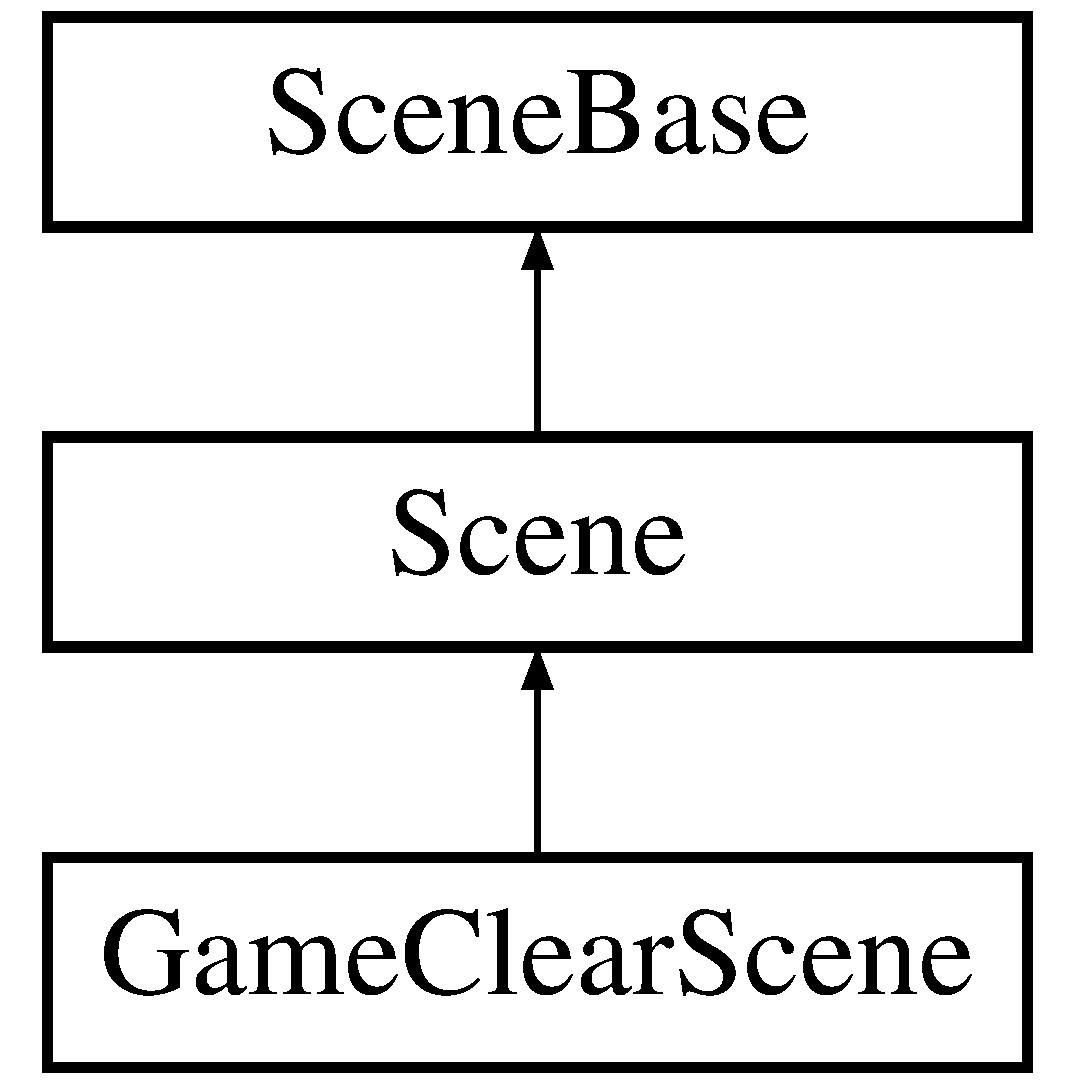
\includegraphics[height=3.000000cm]{class_game_clear_scene}
\end{center}
\end{figure}
\subsection*{公開メンバ関数}
\begin{DoxyCompactItemize}
\item 
void \mbox{\hyperlink{class_game_clear_scene_a59fcf2b5d5d7197d37ecb85c54e7712a}{Init}} () final
\begin{DoxyCompactList}\small\item\em ゲームクリアシーンの初期化 \end{DoxyCompactList}\item 
\mbox{\hyperlink{scene__base_8h_a24cee5343fb9d0706ead6e8601f363be}{S\+C\+E\+NE}} \mbox{\hyperlink{class_game_clear_scene_aebea5913506cc86d9570b286e69dfedd}{Update}} () final
\begin{DoxyCompactList}\small\item\em ゲームクリアシーンの更新 \end{DoxyCompactList}\item 
void \mbox{\hyperlink{class_game_clear_scene_addea514045f47860cfa23439b7bba075}{Render}} () final
\begin{DoxyCompactList}\small\item\em ゲームクリアシーンの描画 \end{DoxyCompactList}\item 
void \mbox{\hyperlink{class_game_clear_scene_a5a3a9e62bb0244b164d9e34663e99594}{Destroy}} () final
\begin{DoxyCompactList}\small\item\em ゲームクリアシーンの破棄 \end{DoxyCompactList}\end{DoxyCompactItemize}
\subsection*{その他の継承メンバ}


\subsection{詳解}
ゲームクリアクラス 

\subsection{関数詳解}
\mbox{\Hypertarget{class_game_clear_scene_a5a3a9e62bb0244b164d9e34663e99594}\label{class_game_clear_scene_a5a3a9e62bb0244b164d9e34663e99594}} 
\index{Game\+Clear\+Scene@{Game\+Clear\+Scene}!Destroy@{Destroy}}
\index{Destroy@{Destroy}!Game\+Clear\+Scene@{Game\+Clear\+Scene}}
\subsubsection{\texorpdfstring{Destroy()}{Destroy()}}
{\footnotesize\ttfamily void Game\+Clear\+Scene\+::\+Destroy (\begin{DoxyParamCaption}{ }\end{DoxyParamCaption})\hspace{0.3cm}{\ttfamily [final]}, {\ttfamily [virtual]}}



ゲームクリアシーンの破棄 



\mbox{\hyperlink{class_scene_base_a7c5b54020bc519b4dadfe9770d6b27f7}{Scene\+Base}}を実装しています。

\mbox{\Hypertarget{class_game_clear_scene_a59fcf2b5d5d7197d37ecb85c54e7712a}\label{class_game_clear_scene_a59fcf2b5d5d7197d37ecb85c54e7712a}} 
\index{Game\+Clear\+Scene@{Game\+Clear\+Scene}!Init@{Init}}
\index{Init@{Init}!Game\+Clear\+Scene@{Game\+Clear\+Scene}}
\subsubsection{\texorpdfstring{Init()}{Init()}}
{\footnotesize\ttfamily void Game\+Clear\+Scene\+::\+Init (\begin{DoxyParamCaption}{ }\end{DoxyParamCaption})\hspace{0.3cm}{\ttfamily [final]}, {\ttfamily [virtual]}}



ゲームクリアシーンの初期化 



\mbox{\hyperlink{class_scene_base_a24d7db43c819924dc8b07b436f6d3148}{Scene\+Base}}を実装しています。

\mbox{\Hypertarget{class_game_clear_scene_addea514045f47860cfa23439b7bba075}\label{class_game_clear_scene_addea514045f47860cfa23439b7bba075}} 
\index{Game\+Clear\+Scene@{Game\+Clear\+Scene}!Render@{Render}}
\index{Render@{Render}!Game\+Clear\+Scene@{Game\+Clear\+Scene}}
\subsubsection{\texorpdfstring{Render()}{Render()}}
{\footnotesize\ttfamily void Game\+Clear\+Scene\+::\+Render (\begin{DoxyParamCaption}{ }\end{DoxyParamCaption})\hspace{0.3cm}{\ttfamily [final]}, {\ttfamily [virtual]}}



ゲームクリアシーンの描画 



\mbox{\hyperlink{class_scene_base_ad981674ce731ea267f398e889bbb9dc3}{Scene\+Base}}を実装しています。

\mbox{\Hypertarget{class_game_clear_scene_aebea5913506cc86d9570b286e69dfedd}\label{class_game_clear_scene_aebea5913506cc86d9570b286e69dfedd}} 
\index{Game\+Clear\+Scene@{Game\+Clear\+Scene}!Update@{Update}}
\index{Update@{Update}!Game\+Clear\+Scene@{Game\+Clear\+Scene}}
\subsubsection{\texorpdfstring{Update()}{Update()}}
{\footnotesize\ttfamily \mbox{\hyperlink{scene__base_8h_a24cee5343fb9d0706ead6e8601f363be}{S\+C\+E\+NE}} Game\+Clear\+Scene\+::\+Update (\begin{DoxyParamCaption}{ }\end{DoxyParamCaption})\hspace{0.3cm}{\ttfamily [final]}, {\ttfamily [virtual]}}



ゲームクリアシーンの更新 

\begin{DoxyReturn}{戻り値}
S\+C\+E\+NE シーンが変わるなら次のシーンのenum classを返す 
\end{DoxyReturn}


\mbox{\hyperlink{class_scene_acb50f8104e5a7cfecbdececa7d5f1b39}{Scene}}を実装しています。



このクラス詳解は次のファイルから抽出されました\+:\begin{DoxyCompactItemize}
\item 
C\+:/\+Users/tokir/\+Documents/\+Git\+Hub/\+Weapon\+Merchant\+Adventure/src/scene/main/clear/\mbox{\hyperlink{game__clear_8h}{game\+\_\+clear.\+h}}\item 
C\+:/\+Users/tokir/\+Documents/\+Git\+Hub/\+Weapon\+Merchant\+Adventure/src/scene/main/clear/\mbox{\hyperlink{game__clear_8cpp}{game\+\_\+clear.\+cpp}}\end{DoxyCompactItemize}

\hypertarget{class_game_over_scene}{}\section{Game\+Over\+Scene クラス}
\label{class_game_over_scene}\index{Game\+Over\+Scene@{Game\+Over\+Scene}}


{\ttfamily \#include $<$game\+\_\+over.\+h$>$}

Game\+Over\+Scene の継承関係図\begin{figure}[H]
\begin{center}
\leavevmode
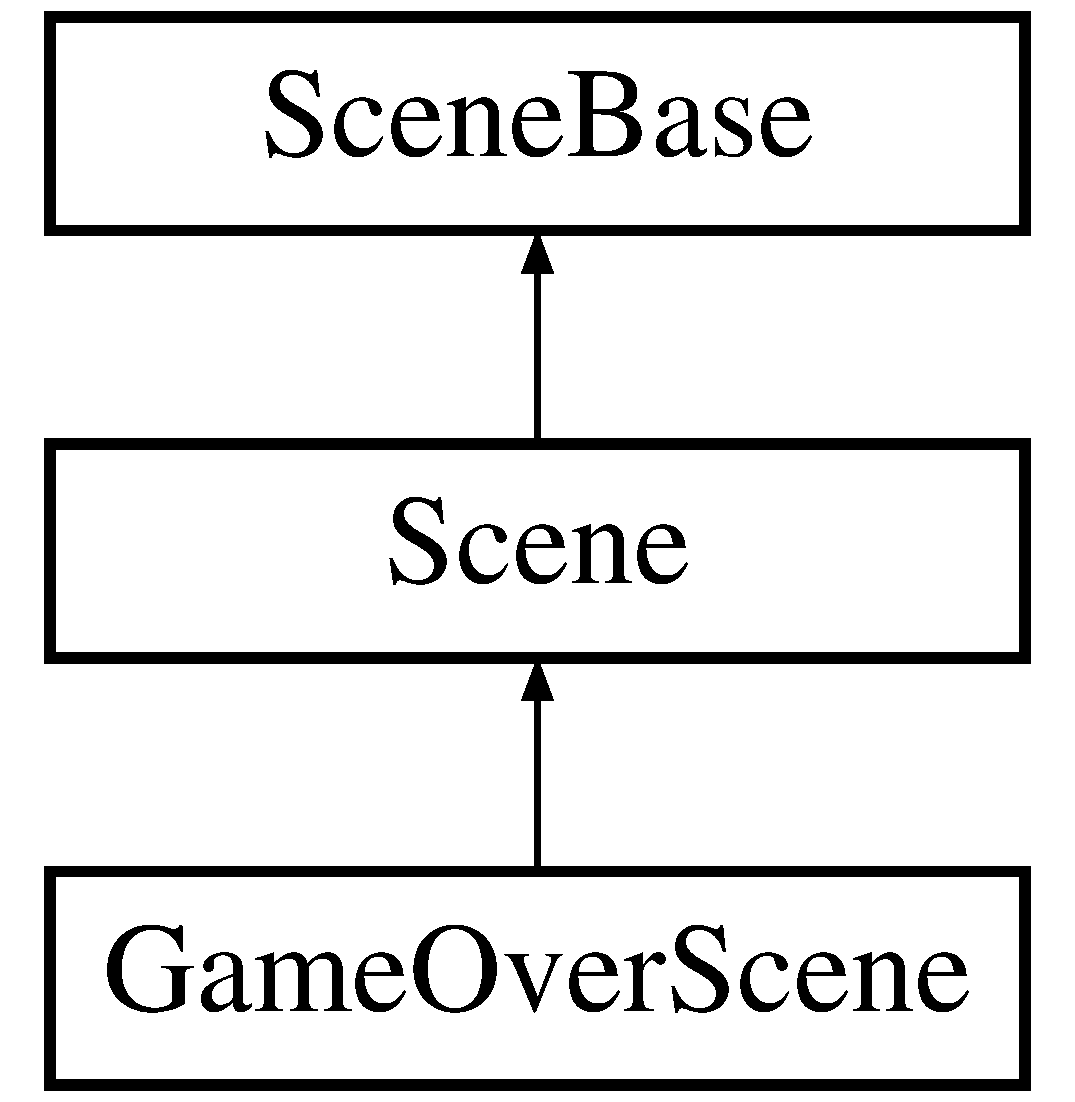
\includegraphics[height=3.000000cm]{class_game_over_scene}
\end{center}
\end{figure}
\subsection*{公開メンバ関数}
\begin{DoxyCompactItemize}
\item 
void \mbox{\hyperlink{class_game_over_scene_a7382331efb2eda768c093f66395655d7}{Init}} () final
\begin{DoxyCompactList}\small\item\em ゲームオーバーシーンの初期化 \end{DoxyCompactList}\item 
\mbox{\hyperlink{scene__base_8h_a24cee5343fb9d0706ead6e8601f363be}{S\+C\+E\+NE}} \mbox{\hyperlink{class_game_over_scene_a27d347ed1ff81cbd252e3bcc3f2989a8}{Update}} () final
\begin{DoxyCompactList}\small\item\em ゲームオーバーシーンの更新 \end{DoxyCompactList}\item 
void \mbox{\hyperlink{class_game_over_scene_a3fd3123c8660c25b01ca2f1e16615072}{Render}} () final
\begin{DoxyCompactList}\small\item\em ゲームオーバーシーンの描画 \end{DoxyCompactList}\item 
void \mbox{\hyperlink{class_game_over_scene_a439e4c515c9549abd6eb45f2a3d115fa}{Destroy}} () final
\begin{DoxyCompactList}\small\item\em ゲームオーバーシーンの破棄 \end{DoxyCompactList}\end{DoxyCompactItemize}
\subsection*{その他の継承メンバ}


\subsection{関数詳解}
\mbox{\Hypertarget{class_game_over_scene_a439e4c515c9549abd6eb45f2a3d115fa}\label{class_game_over_scene_a439e4c515c9549abd6eb45f2a3d115fa}} 
\index{Game\+Over\+Scene@{Game\+Over\+Scene}!Destroy@{Destroy}}
\index{Destroy@{Destroy}!Game\+Over\+Scene@{Game\+Over\+Scene}}
\subsubsection{\texorpdfstring{Destroy()}{Destroy()}}
{\footnotesize\ttfamily void Game\+Over\+Scene\+::\+Destroy (\begin{DoxyParamCaption}{ }\end{DoxyParamCaption})\hspace{0.3cm}{\ttfamily [final]}, {\ttfamily [virtual]}}



ゲームオーバーシーンの破棄 



\mbox{\hyperlink{class_scene_base_a7c5b54020bc519b4dadfe9770d6b27f7}{Scene\+Base}}を実装しています。

\mbox{\Hypertarget{class_game_over_scene_a7382331efb2eda768c093f66395655d7}\label{class_game_over_scene_a7382331efb2eda768c093f66395655d7}} 
\index{Game\+Over\+Scene@{Game\+Over\+Scene}!Init@{Init}}
\index{Init@{Init}!Game\+Over\+Scene@{Game\+Over\+Scene}}
\subsubsection{\texorpdfstring{Init()}{Init()}}
{\footnotesize\ttfamily void Game\+Over\+Scene\+::\+Init (\begin{DoxyParamCaption}{ }\end{DoxyParamCaption})\hspace{0.3cm}{\ttfamily [final]}, {\ttfamily [virtual]}}



ゲームオーバーシーンの初期化 



\mbox{\hyperlink{class_scene_base_a24d7db43c819924dc8b07b436f6d3148}{Scene\+Base}}を実装しています。

\mbox{\Hypertarget{class_game_over_scene_a3fd3123c8660c25b01ca2f1e16615072}\label{class_game_over_scene_a3fd3123c8660c25b01ca2f1e16615072}} 
\index{Game\+Over\+Scene@{Game\+Over\+Scene}!Render@{Render}}
\index{Render@{Render}!Game\+Over\+Scene@{Game\+Over\+Scene}}
\subsubsection{\texorpdfstring{Render()}{Render()}}
{\footnotesize\ttfamily void Game\+Over\+Scene\+::\+Render (\begin{DoxyParamCaption}{ }\end{DoxyParamCaption})\hspace{0.3cm}{\ttfamily [final]}, {\ttfamily [virtual]}}



ゲームオーバーシーンの描画 



\mbox{\hyperlink{class_scene_base_ad981674ce731ea267f398e889bbb9dc3}{Scene\+Base}}を実装しています。

\mbox{\Hypertarget{class_game_over_scene_a27d347ed1ff81cbd252e3bcc3f2989a8}\label{class_game_over_scene_a27d347ed1ff81cbd252e3bcc3f2989a8}} 
\index{Game\+Over\+Scene@{Game\+Over\+Scene}!Update@{Update}}
\index{Update@{Update}!Game\+Over\+Scene@{Game\+Over\+Scene}}
\subsubsection{\texorpdfstring{Update()}{Update()}}
{\footnotesize\ttfamily \mbox{\hyperlink{scene__base_8h_a24cee5343fb9d0706ead6e8601f363be}{S\+C\+E\+NE}} Game\+Over\+Scene\+::\+Update (\begin{DoxyParamCaption}{ }\end{DoxyParamCaption})\hspace{0.3cm}{\ttfamily [final]}, {\ttfamily [virtual]}}



ゲームオーバーシーンの更新 

\begin{DoxyReturn}{戻り値}
S\+C\+E\+NE シーンが変わるなら次のシーンのenum classを返す 
\end{DoxyReturn}


\mbox{\hyperlink{class_scene_acb50f8104e5a7cfecbdececa7d5f1b39}{Scene}}を実装しています。



このクラス詳解は次のファイルから抽出されました\+:\begin{DoxyCompactItemize}
\item 
C\+:/\+Users/tokir/\+Documents/\+Git\+Hub/\+Weapon\+Merchant\+Adventure/src/scene/main/over/\mbox{\hyperlink{game__over_8h}{game\+\_\+over.\+h}}\item 
C\+:/\+Users/tokir/\+Documents/\+Git\+Hub/\+Weapon\+Merchant\+Adventure/src/scene/main/over/\mbox{\hyperlink{game__over_8cpp}{game\+\_\+over.\+cpp}}\end{DoxyCompactItemize}

\hypertarget{class_gamepad_input}{}\section{Gamepad\+Input クラス}
\label{class_gamepad_input}\index{Gamepad\+Input@{Gamepad\+Input}}


ゲームパッドのインプットクラス  




{\ttfamily \#include $<$gamepad\+\_\+input.\+h$>$}

Gamepad\+Input の継承関係図\begin{figure}[H]
\begin{center}
\leavevmode
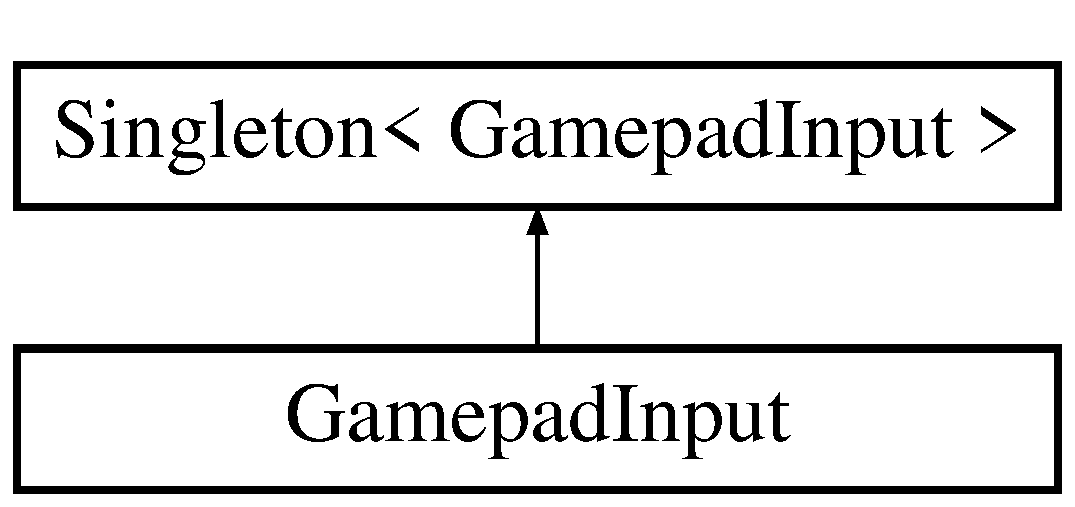
\includegraphics[height=2.000000cm]{class_gamepad_input}
\end{center}
\end{figure}
\subsection*{公開メンバ関数}
\begin{DoxyCompactItemize}
\item 
\mbox{\hyperlink{class_gamepad_input_acd9878326e438f379020827d63ebd6cf}{Gamepad\+Input}} ()
\begin{DoxyCompactList}\small\item\em コンストラクタで初期化 \end{DoxyCompactList}\item 
void \mbox{\hyperlink{class_gamepad_input_a3512c0cc4d57534c83db09c4b5377caa}{Update}} ()
\begin{DoxyCompactList}\small\item\em ゲームパッドインプットの更新 \end{DoxyCompactList}\item 
void \mbox{\hyperlink{class_gamepad_input_afd429d32d076130ff8a7df12037eaddd}{Vibration}} (size\+\_\+t index, float, float)
\begin{DoxyCompactList}\small\item\em コントローラーの振動 \end{DoxyCompactList}\item 
bool \mbox{\hyperlink{class_gamepad_input_a29a71d0503e038e55ffe282e2c768b05}{Get\+Button\+Down}} (size\+\_\+t index, \mbox{\hyperlink{gamepad__input_8h_a739845b0076428add52ca3cec492e705}{B\+U\+T\+T\+ON}} b) const
\begin{DoxyCompactList}\small\item\em --ゲッタ-- \end{DoxyCompactList}\item 
bool \mbox{\hyperlink{class_gamepad_input_a9a2f9042a5fa1c8e33fbd349f67747b3}{Get\+Button}} (size\+\_\+t index, \mbox{\hyperlink{gamepad__input_8h_a739845b0076428add52ca3cec492e705}{B\+U\+T\+T\+ON}} b) const
\begin{DoxyCompactList}\small\item\em ボタンを押しているかどうか \end{DoxyCompactList}\item 
bool \mbox{\hyperlink{class_gamepad_input_a5b76a114b8d3d03abbd2bcd91562109a}{Get\+Button\+Up}} (size\+\_\+t index, \mbox{\hyperlink{gamepad__input_8h_a739845b0076428add52ca3cec492e705}{B\+U\+T\+T\+ON}} b) const
\begin{DoxyCompactList}\small\item\em ボタンを離したかどうか \end{DoxyCompactList}\item 
float \mbox{\hyperlink{class_gamepad_input_a7e95e2a49cbd4729cf7156b9a703252a}{Get\+Trigger}} (size\+\_\+t index, const bool right) const
\begin{DoxyCompactList}\small\item\em トリガーの状態を返す \end{DoxyCompactList}\item 
float \mbox{\hyperlink{class_gamepad_input_a82333353a23ea0fa92bb87d6cf6592d8}{Get\+Stick}} (size\+\_\+t index, const bool right, const bool x) const
\begin{DoxyCompactList}\small\item\em スティックの状態を返す \end{DoxyCompactList}\end{DoxyCompactItemize}
\subsection*{その他の継承メンバ}


\subsection{詳解}
ゲームパッドのインプットクラス 

\subsection{構築子と解体子}
\mbox{\Hypertarget{class_gamepad_input_acd9878326e438f379020827d63ebd6cf}\label{class_gamepad_input_acd9878326e438f379020827d63ebd6cf}} 
\index{Gamepad\+Input@{Gamepad\+Input}!Gamepad\+Input@{Gamepad\+Input}}
\index{Gamepad\+Input@{Gamepad\+Input}!Gamepad\+Input@{Gamepad\+Input}}
\subsubsection{\texorpdfstring{Gamepad\+Input()}{GamepadInput()}}
{\footnotesize\ttfamily Gamepad\+Input\+::\+Gamepad\+Input (\begin{DoxyParamCaption}{ }\end{DoxyParamCaption})}



コンストラクタで初期化 



\subsection{関数詳解}
\mbox{\Hypertarget{class_gamepad_input_a9a2f9042a5fa1c8e33fbd349f67747b3}\label{class_gamepad_input_a9a2f9042a5fa1c8e33fbd349f67747b3}} 
\index{Gamepad\+Input@{Gamepad\+Input}!Get\+Button@{Get\+Button}}
\index{Get\+Button@{Get\+Button}!Gamepad\+Input@{Gamepad\+Input}}
\subsubsection{\texorpdfstring{Get\+Button()}{GetButton()}}
{\footnotesize\ttfamily bool Gamepad\+Input\+::\+Get\+Button (\begin{DoxyParamCaption}\item[{size\+\_\+t}]{index,  }\item[{\mbox{\hyperlink{gamepad__input_8h_a739845b0076428add52ca3cec492e705}{B\+U\+T\+T\+ON}}}]{b }\end{DoxyParamCaption}) const\hspace{0.3cm}{\ttfamily [inline]}}



ボタンを押しているかどうか 


\begin{DoxyParams}{引数}
{\em k} & 判定するボタン \\
\hline
\end{DoxyParams}
\mbox{\Hypertarget{class_gamepad_input_a29a71d0503e038e55ffe282e2c768b05}\label{class_gamepad_input_a29a71d0503e038e55ffe282e2c768b05}} 
\index{Gamepad\+Input@{Gamepad\+Input}!Get\+Button\+Down@{Get\+Button\+Down}}
\index{Get\+Button\+Down@{Get\+Button\+Down}!Gamepad\+Input@{Gamepad\+Input}}
\subsubsection{\texorpdfstring{Get\+Button\+Down()}{GetButtonDown()}}
{\footnotesize\ttfamily bool Gamepad\+Input\+::\+Get\+Button\+Down (\begin{DoxyParamCaption}\item[{size\+\_\+t}]{index,  }\item[{\mbox{\hyperlink{gamepad__input_8h_a739845b0076428add52ca3cec492e705}{B\+U\+T\+T\+ON}}}]{b }\end{DoxyParamCaption}) const\hspace{0.3cm}{\ttfamily [inline]}}



--ゲッタ-- 

ボタンを押したかどうか 
\begin{DoxyParams}{引数}
{\em k} & 判定するボタン \\
\hline
\end{DoxyParams}
\mbox{\Hypertarget{class_gamepad_input_a5b76a114b8d3d03abbd2bcd91562109a}\label{class_gamepad_input_a5b76a114b8d3d03abbd2bcd91562109a}} 
\index{Gamepad\+Input@{Gamepad\+Input}!Get\+Button\+Up@{Get\+Button\+Up}}
\index{Get\+Button\+Up@{Get\+Button\+Up}!Gamepad\+Input@{Gamepad\+Input}}
\subsubsection{\texorpdfstring{Get\+Button\+Up()}{GetButtonUp()}}
{\footnotesize\ttfamily bool Gamepad\+Input\+::\+Get\+Button\+Up (\begin{DoxyParamCaption}\item[{size\+\_\+t}]{index,  }\item[{\mbox{\hyperlink{gamepad__input_8h_a739845b0076428add52ca3cec492e705}{B\+U\+T\+T\+ON}}}]{b }\end{DoxyParamCaption}) const\hspace{0.3cm}{\ttfamily [inline]}}



ボタンを離したかどうか 


\begin{DoxyParams}{引数}
{\em k} & 判定するボタン \\
\hline
\end{DoxyParams}
\mbox{\Hypertarget{class_gamepad_input_a82333353a23ea0fa92bb87d6cf6592d8}\label{class_gamepad_input_a82333353a23ea0fa92bb87d6cf6592d8}} 
\index{Gamepad\+Input@{Gamepad\+Input}!Get\+Stick@{Get\+Stick}}
\index{Get\+Stick@{Get\+Stick}!Gamepad\+Input@{Gamepad\+Input}}
\subsubsection{\texorpdfstring{Get\+Stick()}{GetStick()}}
{\footnotesize\ttfamily float Gamepad\+Input\+::\+Get\+Stick (\begin{DoxyParamCaption}\item[{size\+\_\+t}]{index,  }\item[{const bool}]{right,  }\item[{const bool}]{x }\end{DoxyParamCaption}) const\hspace{0.3cm}{\ttfamily [inline]}}



スティックの状態を返す 


\begin{DoxyParams}{引数}
{\em right} & 判定するのが右かどうか \\
\hline
{\em right} & 判定するのがxかどうか \\
\hline
\end{DoxyParams}
\mbox{\Hypertarget{class_gamepad_input_a7e95e2a49cbd4729cf7156b9a703252a}\label{class_gamepad_input_a7e95e2a49cbd4729cf7156b9a703252a}} 
\index{Gamepad\+Input@{Gamepad\+Input}!Get\+Trigger@{Get\+Trigger}}
\index{Get\+Trigger@{Get\+Trigger}!Gamepad\+Input@{Gamepad\+Input}}
\subsubsection{\texorpdfstring{Get\+Trigger()}{GetTrigger()}}
{\footnotesize\ttfamily float Gamepad\+Input\+::\+Get\+Trigger (\begin{DoxyParamCaption}\item[{size\+\_\+t}]{index,  }\item[{const bool}]{right }\end{DoxyParamCaption}) const\hspace{0.3cm}{\ttfamily [inline]}}



トリガーの状態を返す 


\begin{DoxyParams}{引数}
{\em right} & 判定するのが右かどうか \\
\hline
\end{DoxyParams}
\mbox{\Hypertarget{class_gamepad_input_a3512c0cc4d57534c83db09c4b5377caa}\label{class_gamepad_input_a3512c0cc4d57534c83db09c4b5377caa}} 
\index{Gamepad\+Input@{Gamepad\+Input}!Update@{Update}}
\index{Update@{Update}!Gamepad\+Input@{Gamepad\+Input}}
\subsubsection{\texorpdfstring{Update()}{Update()}}
{\footnotesize\ttfamily void Gamepad\+Input\+::\+Update (\begin{DoxyParamCaption}{ }\end{DoxyParamCaption})}



ゲームパッドインプットの更新 

\mbox{\Hypertarget{class_gamepad_input_afd429d32d076130ff8a7df12037eaddd}\label{class_gamepad_input_afd429d32d076130ff8a7df12037eaddd}} 
\index{Gamepad\+Input@{Gamepad\+Input}!Vibration@{Vibration}}
\index{Vibration@{Vibration}!Gamepad\+Input@{Gamepad\+Input}}
\subsubsection{\texorpdfstring{Vibration()}{Vibration()}}
{\footnotesize\ttfamily void Gamepad\+Input\+::\+Vibration (\begin{DoxyParamCaption}\item[{size\+\_\+t}]{index,  }\item[{float}]{right,  }\item[{float}]{left }\end{DoxyParamCaption})}



コントローラーの振動 


\begin{DoxyParams}{引数}
{\em right} & 右のモーターの力 \\
\hline
{\em left} & 左のモーターの力 \\
\hline
\end{DoxyParams}


このクラス詳解は次のファイルから抽出されました\+:\begin{DoxyCompactItemize}
\item 
C\+:/\+Users/tokir/\+Documents/\+Git\+Hub/\+Weapon\+Merchant\+Adventure/src/src/input/gamepad/\mbox{\hyperlink{gamepad__input_8h}{gamepad\+\_\+input.\+h}}\item 
C\+:/\+Users/tokir/\+Documents/\+Git\+Hub/\+Weapon\+Merchant\+Adventure/src/src/input/gamepad/\mbox{\hyperlink{gamepad__input_8cpp}{gamepad\+\_\+input.\+cpp}}\end{DoxyCompactItemize}

\hypertarget{class_game_scene}{}\section{Game\+Scene クラス}
\label{class_game_scene}\index{Game\+Scene@{Game\+Scene}}


ゲームシーンクラス  




{\ttfamily \#include $<$game\+\_\+scene.\+h$>$}

Game\+Scene の継承関係図\begin{figure}[H]
\begin{center}
\leavevmode
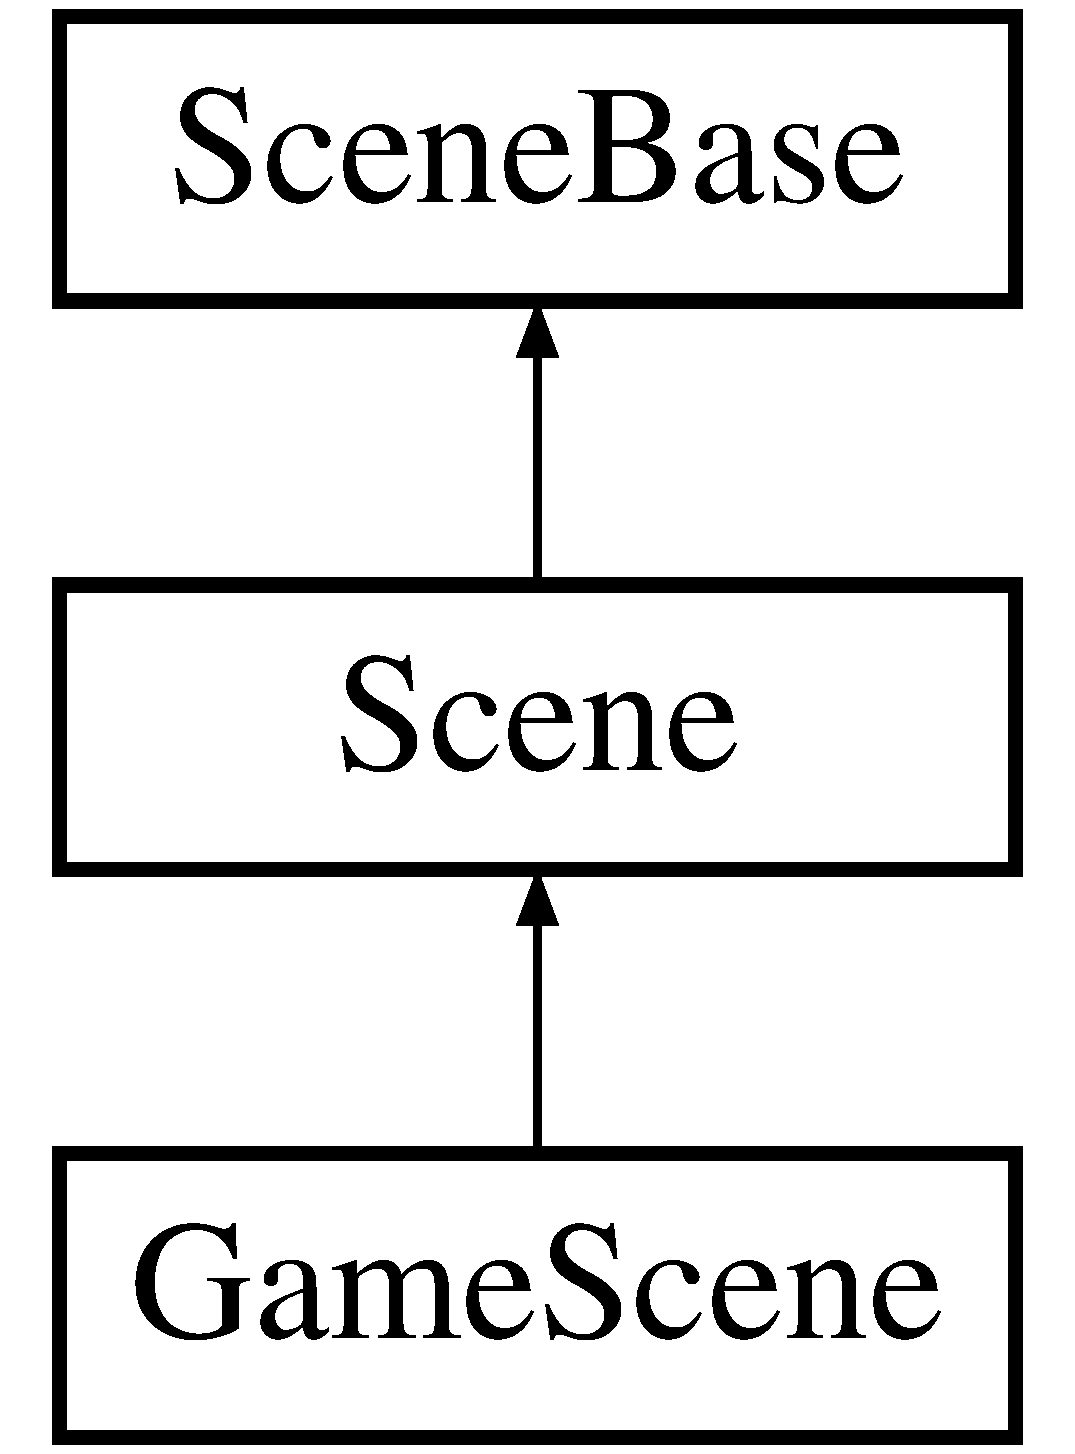
\includegraphics[height=3.000000cm]{class_game_scene}
\end{center}
\end{figure}
\subsection*{公開メンバ関数}
\begin{DoxyCompactItemize}
\item 
void \mbox{\hyperlink{class_game_scene_a86227765def624b9b227db2aa41d9141}{Init}} () final
\begin{DoxyCompactList}\small\item\em ゲームシーンの初期化 \end{DoxyCompactList}\item 
\mbox{\hyperlink{scene__base_8h_a24cee5343fb9d0706ead6e8601f363be}{S\+C\+E\+NE}} \mbox{\hyperlink{class_game_scene_a2d4c44e96484af17ed3f6fb0402ebafd}{Update}} () final
\begin{DoxyCompactList}\small\item\em ゲームシーンの更新 \end{DoxyCompactList}\item 
void \mbox{\hyperlink{class_game_scene_ae5ecfa81aecd5e959b038142640a1c7b}{Render}} () final
\begin{DoxyCompactList}\small\item\em ゲームシーンの描画 \end{DoxyCompactList}\item 
void \mbox{\hyperlink{class_game_scene_a5c544d5a87a60f09ada75f1f60f0a787}{Destroy}} () final
\begin{DoxyCompactList}\small\item\em ゲームシーンの破棄 \end{DoxyCompactList}\end{DoxyCompactItemize}
\subsection*{その他の継承メンバ}


\subsection{詳解}
ゲームシーンクラス 

\subsection{関数詳解}
\mbox{\Hypertarget{class_game_scene_a5c544d5a87a60f09ada75f1f60f0a787}\label{class_game_scene_a5c544d5a87a60f09ada75f1f60f0a787}} 
\index{Game\+Scene@{Game\+Scene}!Destroy@{Destroy}}
\index{Destroy@{Destroy}!Game\+Scene@{Game\+Scene}}
\subsubsection{\texorpdfstring{Destroy()}{Destroy()}}
{\footnotesize\ttfamily void Game\+Scene\+::\+Destroy (\begin{DoxyParamCaption}{ }\end{DoxyParamCaption})\hspace{0.3cm}{\ttfamily [final]}, {\ttfamily [virtual]}}



ゲームシーンの破棄 



\mbox{\hyperlink{class_scene_base_a7c5b54020bc519b4dadfe9770d6b27f7}{Scene\+Base}}を実装しています。

\mbox{\Hypertarget{class_game_scene_a86227765def624b9b227db2aa41d9141}\label{class_game_scene_a86227765def624b9b227db2aa41d9141}} 
\index{Game\+Scene@{Game\+Scene}!Init@{Init}}
\index{Init@{Init}!Game\+Scene@{Game\+Scene}}
\subsubsection{\texorpdfstring{Init()}{Init()}}
{\footnotesize\ttfamily void Game\+Scene\+::\+Init (\begin{DoxyParamCaption}{ }\end{DoxyParamCaption})\hspace{0.3cm}{\ttfamily [final]}, {\ttfamily [virtual]}}



ゲームシーンの初期化 



\mbox{\hyperlink{class_scene_base_a24d7db43c819924dc8b07b436f6d3148}{Scene\+Base}}を実装しています。

\mbox{\Hypertarget{class_game_scene_ae5ecfa81aecd5e959b038142640a1c7b}\label{class_game_scene_ae5ecfa81aecd5e959b038142640a1c7b}} 
\index{Game\+Scene@{Game\+Scene}!Render@{Render}}
\index{Render@{Render}!Game\+Scene@{Game\+Scene}}
\subsubsection{\texorpdfstring{Render()}{Render()}}
{\footnotesize\ttfamily void Game\+Scene\+::\+Render (\begin{DoxyParamCaption}{ }\end{DoxyParamCaption})\hspace{0.3cm}{\ttfamily [final]}, {\ttfamily [virtual]}}



ゲームシーンの描画 



\mbox{\hyperlink{class_scene_base_ad981674ce731ea267f398e889bbb9dc3}{Scene\+Base}}を実装しています。

\mbox{\Hypertarget{class_game_scene_a2d4c44e96484af17ed3f6fb0402ebafd}\label{class_game_scene_a2d4c44e96484af17ed3f6fb0402ebafd}} 
\index{Game\+Scene@{Game\+Scene}!Update@{Update}}
\index{Update@{Update}!Game\+Scene@{Game\+Scene}}
\subsubsection{\texorpdfstring{Update()}{Update()}}
{\footnotesize\ttfamily \mbox{\hyperlink{scene__base_8h_a24cee5343fb9d0706ead6e8601f363be}{S\+C\+E\+NE}} Game\+Scene\+::\+Update (\begin{DoxyParamCaption}{ }\end{DoxyParamCaption})\hspace{0.3cm}{\ttfamily [final]}, {\ttfamily [virtual]}}



ゲームシーンの更新 

\begin{DoxyReturn}{戻り値}
S\+C\+E\+NE シーンが変わるなら次のシーンのenum classを返す 
\end{DoxyReturn}


\mbox{\hyperlink{class_scene_acb50f8104e5a7cfecbdececa7d5f1b39}{Scene}}を実装しています。



このクラス詳解は次のファイルから抽出されました\+:\begin{DoxyCompactItemize}
\item 
C\+:/\+Users/tokir/\+Documents/\+Git\+Hub/\+Weapon\+Merchant\+Adventure/src/scene/main/game/\mbox{\hyperlink{game__scene_8h}{game\+\_\+scene.\+h}}\item 
C\+:/\+Users/tokir/\+Documents/\+Git\+Hub/\+Weapon\+Merchant\+Adventure/src/scene/main/game/\mbox{\hyperlink{game__scene_8cpp}{game\+\_\+scene.\+cpp}}\end{DoxyCompactItemize}

\hypertarget{class_gravity}{}\section{Gravity クラス}
\label{class_gravity}\index{Gravity@{Gravity}}


重力を管理するクラス  




{\ttfamily \#include $<$gravity.\+h$>$}

\subsection*{公開メンバ関数}
\begin{DoxyCompactItemize}
\item 
float \mbox{\hyperlink{class_gravity_a4af84c9743d47601d92c83534af7b55f}{Add\+Gravity}} ()
\begin{DoxyCompactList}\small\item\em 重力の追加 \end{DoxyCompactList}\item 
void \mbox{\hyperlink{class_gravity_a5cc5e47fc7c323ea38a2a289bdefae51}{Set\+Power}} (const float \+\_\+power)
\begin{DoxyCompactList}\small\item\em 加速度のセット \end{DoxyCompactList}\item 
void \mbox{\hyperlink{class_gravity_aa334a7ebbbd79ca28e7d29c3fc5c03ed}{Reset\+Gravity}} ()
\end{DoxyCompactItemize}


\subsection{詳解}
重力を管理するクラス 

\subsection{関数詳解}
\mbox{\Hypertarget{class_gravity_a4af84c9743d47601d92c83534af7b55f}\label{class_gravity_a4af84c9743d47601d92c83534af7b55f}} 
\index{Gravity@{Gravity}!Add\+Gravity@{Add\+Gravity}}
\index{Add\+Gravity@{Add\+Gravity}!Gravity@{Gravity}}
\subsubsection{\texorpdfstring{Add\+Gravity()}{AddGravity()}}
{\footnotesize\ttfamily float Gravity\+::\+Add\+Gravity (\begin{DoxyParamCaption}{ }\end{DoxyParamCaption})}



重力の追加 

\mbox{\Hypertarget{class_gravity_aa334a7ebbbd79ca28e7d29c3fc5c03ed}\label{class_gravity_aa334a7ebbbd79ca28e7d29c3fc5c03ed}} 
\index{Gravity@{Gravity}!Reset\+Gravity@{Reset\+Gravity}}
\index{Reset\+Gravity@{Reset\+Gravity}!Gravity@{Gravity}}
\subsubsection{\texorpdfstring{Reset\+Gravity()}{ResetGravity()}}
{\footnotesize\ttfamily void Gravity\+::\+Reset\+Gravity (\begin{DoxyParamCaption}{ }\end{DoxyParamCaption})\hspace{0.3cm}{\ttfamily [inline]}}


\begin{DoxyParams}{引数}
{\em 重力系のリセット} & \\
\hline
\end{DoxyParams}
\mbox{\Hypertarget{class_gravity_a5cc5e47fc7c323ea38a2a289bdefae51}\label{class_gravity_a5cc5e47fc7c323ea38a2a289bdefae51}} 
\index{Gravity@{Gravity}!Set\+Power@{Set\+Power}}
\index{Set\+Power@{Set\+Power}!Gravity@{Gravity}}
\subsubsection{\texorpdfstring{Set\+Power()}{SetPower()}}
{\footnotesize\ttfamily void Gravity\+::\+Set\+Power (\begin{DoxyParamCaption}\item[{const float}]{\+\_\+power }\end{DoxyParamCaption})\hspace{0.3cm}{\ttfamily [inline]}}



加速度のセット 


\begin{DoxyParams}{引数}
{\em 加速度} & \\
\hline
\end{DoxyParams}


このクラス詳解は次のファイルから抽出されました\+:\begin{DoxyCompactItemize}
\item 
C\+:/\+Users/tokir/\+Documents/\+Git\+Hub/\+Weapon\+Merchant\+Adventure/src/gravity/\mbox{\hyperlink{gravity_8h}{gravity.\+h}}\item 
C\+:/\+Users/tokir/\+Documents/\+Git\+Hub/\+Weapon\+Merchant\+Adventure/src/gravity/\mbox{\hyperlink{gravity_8cpp}{gravity.\+cpp}}\end{DoxyCompactItemize}

\hypertarget{class_map_object}{}\section{Map\+Object クラス}
\label{class_map_object}\index{Map\+Object@{Map\+Object}}


マップに配置するオブジェクトのクラス  




{\ttfamily \#include $<$map.\+h$>$}

Map\+Object の継承関係図\begin{figure}[H]
\begin{center}
\leavevmode
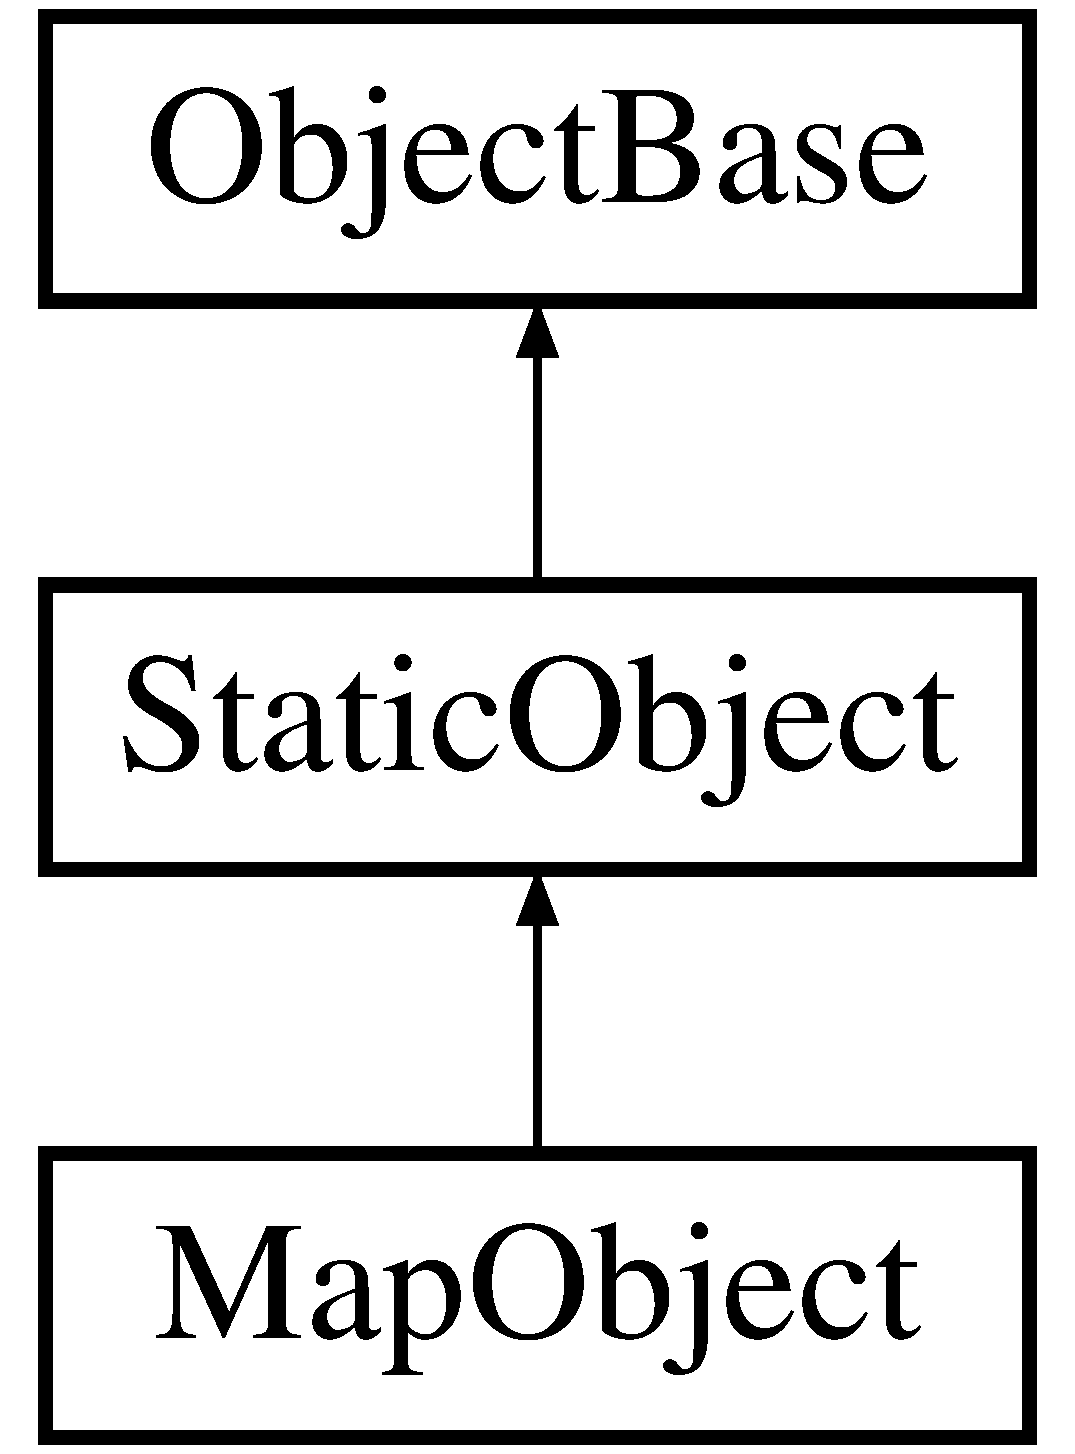
\includegraphics[height=3.000000cm]{class_map_object}
\end{center}
\end{figure}
\subsection*{公開メンバ関数}
\begin{DoxyCompactItemize}
\item 
void \mbox{\hyperlink{class_map_object_ad4bcfdc33bd945a9aa5e50a57c2704bc}{Destroy}} () final
\begin{DoxyCompactList}\small\item\em マップの破棄 \end{DoxyCompactList}\item 
\mbox{\hyperlink{class_map_object_a568754515cc72ce0861d30c3040d26d2}{Map\+Object}} ()
\begin{DoxyCompactList}\small\item\em コンストラクタ \end{DoxyCompactList}\item 
\mbox{\hyperlink{class_map_object_a4d69915b6837056e40c0c17afe78ce8e}{Map\+Object}} (const \mbox{\hyperlink{class_map_object}{Map\+Object}} \&m)
\begin{DoxyCompactList}\small\item\em コピーコンストラクタ \end{DoxyCompactList}\item 
\mbox{\hyperlink{class_map_object_ad3779307ee41c0bc0fdf4b419baac3da}{Map\+Object}} (\mbox{\hyperlink{class_map_object}{Map\+Object}} \&\&m) noexcept
\begin{DoxyCompactList}\small\item\em ムーブコンストラクタ \end{DoxyCompactList}\item 
\mbox{\hyperlink{class_map_object}{Map\+Object}} \& \mbox{\hyperlink{class_map_object_a4ff3c31cc463a650e4d870ea65b65c58}{operator=}} (const \mbox{\hyperlink{class_map_object}{Map\+Object}} \&other)
\begin{DoxyCompactList}\small\item\em コピー代入演算子 \end{DoxyCompactList}\item 
\mbox{\hyperlink{class_map_object}{Map\+Object}} \& \mbox{\hyperlink{class_map_object_ae36fa838f3f8bac8ef2d67b39adf0298}{operator=}} (\mbox{\hyperlink{class_map_object}{Map\+Object}} \&\&other) noexcept
\begin{DoxyCompactList}\small\item\em ムーブ代入演算子 \end{DoxyCompactList}\item 
void \mbox{\hyperlink{class_map_object_a76b9161f2723272ad361d0b190e46245}{Collision}} (\mbox{\hyperlink{class_object_base}{Object\+Base}} $\ast$, \mbox{\hyperlink{common_8h_ae148fff5818e9444b4ab2288829559bf}{Vec2}}) final
\begin{DoxyCompactList}\small\item\em マップが当たってるときに実行する関数 \end{DoxyCompactList}\item 
\mbox{\hyperlink{class_map_object_aa601344267a49df197e841fcbd732209}{$\sim$\+Map\+Object}} ()
\begin{DoxyCompactList}\small\item\em デストラクタ \end{DoxyCompactList}\end{DoxyCompactItemize}
\subsection*{公開変数類}
\begin{DoxyCompactItemize}
\item 
bool \mbox{\hyperlink{class_map_object_a21c5d70f23cca2a184297d766cc6acdc}{is\+\_\+mapchip}} = true
\end{DoxyCompactItemize}
\subsection*{限定公開メンバ関数}
\begin{DoxyCompactItemize}
\item 
void \mbox{\hyperlink{class_map_object_a3043cddb8aaad0eab27a076e9bee0284}{Init\+Process}} () final
\begin{DoxyCompactList}\small\item\em 初期化 \end{DoxyCompactList}\item 
void \mbox{\hyperlink{class_map_object_ab6b8849f15175417eca94b2703945e4b}{Update\+Process}} () final
\begin{DoxyCompactList}\small\item\em マップの更新 \end{DoxyCompactList}\end{DoxyCompactItemize}
\subsection*{その他の継承メンバ}


\subsection{詳解}
マップに配置するオブジェクトのクラス 

\subsection{構築子と解体子}
\mbox{\Hypertarget{class_map_object_a568754515cc72ce0861d30c3040d26d2}\label{class_map_object_a568754515cc72ce0861d30c3040d26d2}} 
\index{Map\+Object@{Map\+Object}!Map\+Object@{Map\+Object}}
\index{Map\+Object@{Map\+Object}!Map\+Object@{Map\+Object}}
\subsubsection{\texorpdfstring{Map\+Object()}{MapObject()}\hspace{0.1cm}{\footnotesize\ttfamily [1/3]}}
{\footnotesize\ttfamily Map\+Object\+::\+Map\+Object (\begin{DoxyParamCaption}{ }\end{DoxyParamCaption})\hspace{0.3cm}{\ttfamily [inline]}}



コンストラクタ 

\mbox{\Hypertarget{class_map_object_a4d69915b6837056e40c0c17afe78ce8e}\label{class_map_object_a4d69915b6837056e40c0c17afe78ce8e}} 
\index{Map\+Object@{Map\+Object}!Map\+Object@{Map\+Object}}
\index{Map\+Object@{Map\+Object}!Map\+Object@{Map\+Object}}
\subsubsection{\texorpdfstring{Map\+Object()}{MapObject()}\hspace{0.1cm}{\footnotesize\ttfamily [2/3]}}
{\footnotesize\ttfamily Map\+Object\+::\+Map\+Object (\begin{DoxyParamCaption}\item[{const \mbox{\hyperlink{class_map_object}{Map\+Object}} \&}]{m }\end{DoxyParamCaption})\hspace{0.3cm}{\ttfamily [inline]}}



コピーコンストラクタ 

\mbox{\Hypertarget{class_map_object_ad3779307ee41c0bc0fdf4b419baac3da}\label{class_map_object_ad3779307ee41c0bc0fdf4b419baac3da}} 
\index{Map\+Object@{Map\+Object}!Map\+Object@{Map\+Object}}
\index{Map\+Object@{Map\+Object}!Map\+Object@{Map\+Object}}
\subsubsection{\texorpdfstring{Map\+Object()}{MapObject()}\hspace{0.1cm}{\footnotesize\ttfamily [3/3]}}
{\footnotesize\ttfamily Map\+Object\+::\+Map\+Object (\begin{DoxyParamCaption}\item[{\mbox{\hyperlink{class_map_object}{Map\+Object}} \&\&}]{m }\end{DoxyParamCaption})\hspace{0.3cm}{\ttfamily [inline]}, {\ttfamily [noexcept]}}



ムーブコンストラクタ 

\mbox{\Hypertarget{class_map_object_aa601344267a49df197e841fcbd732209}\label{class_map_object_aa601344267a49df197e841fcbd732209}} 
\index{Map\+Object@{Map\+Object}!````~Map\+Object@{$\sim$\+Map\+Object}}
\index{````~Map\+Object@{$\sim$\+Map\+Object}!Map\+Object@{Map\+Object}}
\subsubsection{\texorpdfstring{$\sim$\+Map\+Object()}{~MapObject()}}
{\footnotesize\ttfamily Map\+Object\+::$\sim$\+Map\+Object (\begin{DoxyParamCaption}{ }\end{DoxyParamCaption})\hspace{0.3cm}{\ttfamily [inline]}}



デストラクタ 



\subsection{関数詳解}
\mbox{\Hypertarget{class_map_object_a76b9161f2723272ad361d0b190e46245}\label{class_map_object_a76b9161f2723272ad361d0b190e46245}} 
\index{Map\+Object@{Map\+Object}!Collision@{Collision}}
\index{Collision@{Collision}!Map\+Object@{Map\+Object}}
\subsubsection{\texorpdfstring{Collision()}{Collision()}}
{\footnotesize\ttfamily void Map\+Object\+::\+Collision (\begin{DoxyParamCaption}\item[{\mbox{\hyperlink{class_object_base}{Object\+Base}} $\ast$}]{obj,  }\item[{\mbox{\hyperlink{common_8h_ae148fff5818e9444b4ab2288829559bf}{Vec2}}}]{ }\end{DoxyParamCaption})\hspace{0.3cm}{\ttfamily [final]}, {\ttfamily [virtual]}}



マップが当たってるときに実行する関数 



\mbox{\hyperlink{class_static_object_a64c8803ff881d578d103413e299dbf7f}{Static\+Object}}を再実装しています。

\mbox{\Hypertarget{class_map_object_ad4bcfdc33bd945a9aa5e50a57c2704bc}\label{class_map_object_ad4bcfdc33bd945a9aa5e50a57c2704bc}} 
\index{Map\+Object@{Map\+Object}!Destroy@{Destroy}}
\index{Destroy@{Destroy}!Map\+Object@{Map\+Object}}
\subsubsection{\texorpdfstring{Destroy()}{Destroy()}}
{\footnotesize\ttfamily void Map\+Object\+::\+Destroy (\begin{DoxyParamCaption}{ }\end{DoxyParamCaption})\hspace{0.3cm}{\ttfamily [final]}, {\ttfamily [virtual]}}



マップの破棄 



\mbox{\hyperlink{class_static_object_a8e9fb321b4f8f12c4bec1bc66853512f}{Static\+Object}}を再実装しています。

\mbox{\Hypertarget{class_map_object_a3043cddb8aaad0eab27a076e9bee0284}\label{class_map_object_a3043cddb8aaad0eab27a076e9bee0284}} 
\index{Map\+Object@{Map\+Object}!Init\+Process@{Init\+Process}}
\index{Init\+Process@{Init\+Process}!Map\+Object@{Map\+Object}}
\subsubsection{\texorpdfstring{Init\+Process()}{InitProcess()}}
{\footnotesize\ttfamily void Map\+Object\+::\+Init\+Process (\begin{DoxyParamCaption}{ }\end{DoxyParamCaption})\hspace{0.3cm}{\ttfamily [final]}, {\ttfamily [protected]}, {\ttfamily [virtual]}}



初期化 



\mbox{\hyperlink{class_static_object_afa0709f50495338a23c1140062a567af}{Static\+Object}}を再実装しています。

\mbox{\Hypertarget{class_map_object_a4ff3c31cc463a650e4d870ea65b65c58}\label{class_map_object_a4ff3c31cc463a650e4d870ea65b65c58}} 
\index{Map\+Object@{Map\+Object}!operator=@{operator=}}
\index{operator=@{operator=}!Map\+Object@{Map\+Object}}
\subsubsection{\texorpdfstring{operator=()}{operator=()}\hspace{0.1cm}{\footnotesize\ttfamily [1/2]}}
{\footnotesize\ttfamily \mbox{\hyperlink{class_map_object}{Map\+Object}}\& Map\+Object\+::operator= (\begin{DoxyParamCaption}\item[{const \mbox{\hyperlink{class_map_object}{Map\+Object}} \&}]{other }\end{DoxyParamCaption})\hspace{0.3cm}{\ttfamily [inline]}}



コピー代入演算子 

\mbox{\Hypertarget{class_map_object_ae36fa838f3f8bac8ef2d67b39adf0298}\label{class_map_object_ae36fa838f3f8bac8ef2d67b39adf0298}} 
\index{Map\+Object@{Map\+Object}!operator=@{operator=}}
\index{operator=@{operator=}!Map\+Object@{Map\+Object}}
\subsubsection{\texorpdfstring{operator=()}{operator=()}\hspace{0.1cm}{\footnotesize\ttfamily [2/2]}}
{\footnotesize\ttfamily \mbox{\hyperlink{class_map_object}{Map\+Object}}\& Map\+Object\+::operator= (\begin{DoxyParamCaption}\item[{\mbox{\hyperlink{class_map_object}{Map\+Object}} \&\&}]{other }\end{DoxyParamCaption})\hspace{0.3cm}{\ttfamily [inline]}, {\ttfamily [noexcept]}}



ムーブ代入演算子 

\mbox{\Hypertarget{class_map_object_ab6b8849f15175417eca94b2703945e4b}\label{class_map_object_ab6b8849f15175417eca94b2703945e4b}} 
\index{Map\+Object@{Map\+Object}!Update\+Process@{Update\+Process}}
\index{Update\+Process@{Update\+Process}!Map\+Object@{Map\+Object}}
\subsubsection{\texorpdfstring{Update\+Process()}{UpdateProcess()}}
{\footnotesize\ttfamily void Map\+Object\+::\+Update\+Process (\begin{DoxyParamCaption}{ }\end{DoxyParamCaption})\hspace{0.3cm}{\ttfamily [final]}, {\ttfamily [protected]}, {\ttfamily [virtual]}}



マップの更新 



\mbox{\hyperlink{class_static_object_a7fa678c3c4032bb6e9417f93a8bb895c}{Static\+Object}}を再実装しています。



\subsection{メンバ詳解}
\mbox{\Hypertarget{class_map_object_a21c5d70f23cca2a184297d766cc6acdc}\label{class_map_object_a21c5d70f23cca2a184297d766cc6acdc}} 
\index{Map\+Object@{Map\+Object}!is\+\_\+mapchip@{is\+\_\+mapchip}}
\index{is\+\_\+mapchip@{is\+\_\+mapchip}!Map\+Object@{Map\+Object}}
\subsubsection{\texorpdfstring{is\+\_\+mapchip}{is\_mapchip}}
{\footnotesize\ttfamily bool Map\+Object\+::is\+\_\+mapchip = true}



このクラス詳解は次のファイルから抽出されました\+:\begin{DoxyCompactItemize}
\item 
C\+:/\+Users/tokir/\+Documents/\+Git\+Hub/\+Weapon\+Merchant\+Adventure/src/src/object/map/\mbox{\hyperlink{map_8h}{map.\+h}}\item 
C\+:/\+Users/tokir/\+Documents/\+Git\+Hub/\+Weapon\+Merchant\+Adventure/src/src/object/map/\mbox{\hyperlink{map_8cpp}{map.\+cpp}}\end{DoxyCompactItemize}

\hypertarget{class_normal_enemy}{}\section{Normal\+Enemy クラス}
\label{class_normal_enemy}\index{Normal\+Enemy@{Normal\+Enemy}}


ノーマルな敵クラス  




{\ttfamily \#include $<$normal\+\_\+enemy.\+h$>$}

Normal\+Enemy の継承関係図\begin{figure}[H]
\begin{center}
\leavevmode
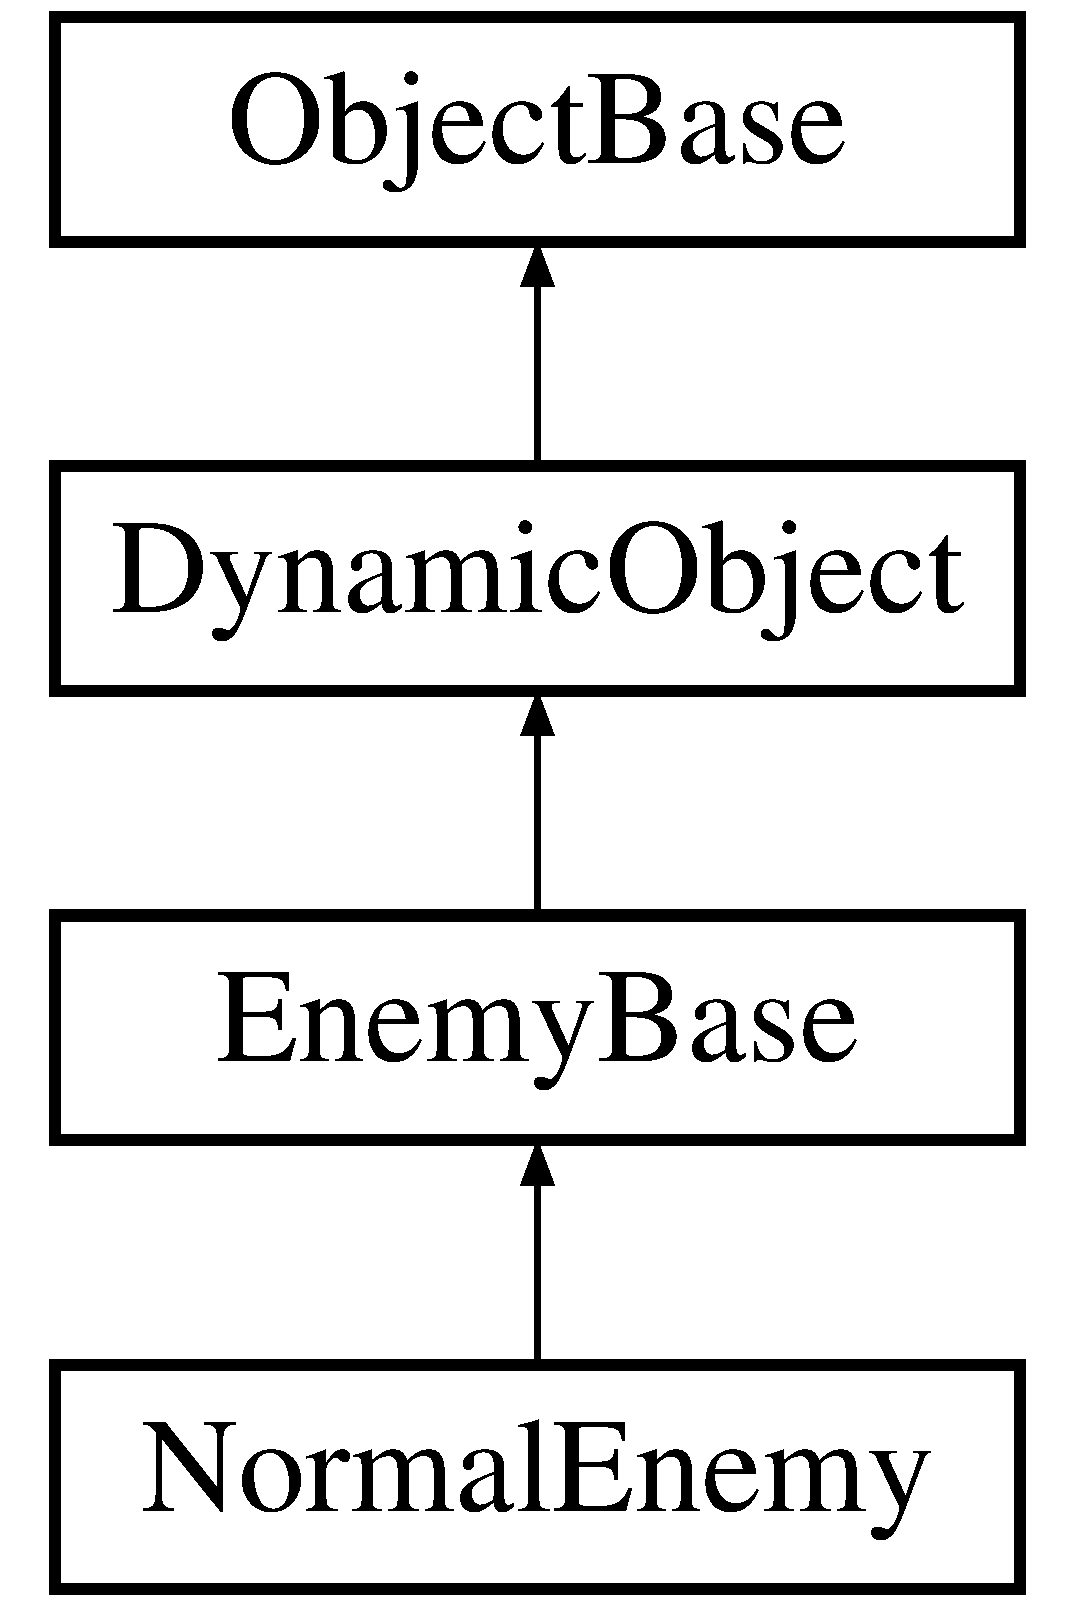
\includegraphics[height=4.000000cm]{class_normal_enemy}
\end{center}
\end{figure}
\subsection*{公開メンバ関数}
\begin{DoxyCompactItemize}
\item 
\mbox{\hyperlink{class_normal_enemy_aa386eea59a2983574fe7d55a91f93012}{Normal\+Enemy}} ()
\begin{DoxyCompactList}\small\item\em コンストラクタ \end{DoxyCompactList}\item 
\mbox{\hyperlink{class_normal_enemy_a08bfcea97297d0cff5c10854c8f5ffb8}{Normal\+Enemy}} (const \mbox{\hyperlink{class_normal_enemy}{Normal\+Enemy}} \&ne)
\begin{DoxyCompactList}\small\item\em コピーコンストラクタ \end{DoxyCompactList}\item 
\mbox{\hyperlink{class_normal_enemy_a64edfeecedfae67d33a5e1fcdccbbfa6}{Normal\+Enemy}} (\mbox{\hyperlink{class_normal_enemy}{Normal\+Enemy}} \&\&ne) noexcept
\begin{DoxyCompactList}\small\item\em ムーブコンストラクタ \end{DoxyCompactList}\item 
\mbox{\hyperlink{class_normal_enemy}{Normal\+Enemy}} \& \mbox{\hyperlink{class_normal_enemy_a4294020d85d9ae77a47294e04fd048b6}{operator=}} (const \mbox{\hyperlink{class_normal_enemy}{Normal\+Enemy}} \&other)
\begin{DoxyCompactList}\small\item\em コピー代入演算子 \end{DoxyCompactList}\item 
void \mbox{\hyperlink{class_normal_enemy_a71cb11fe60d713ce638dcec5d66912e6}{Collision}} (\mbox{\hyperlink{class_object_base}{Object\+Base}} $\ast$, \mbox{\hyperlink{common_8h_ae148fff5818e9444b4ab2288829559bf}{Vec2}}) final
\begin{DoxyCompactList}\small\item\em エネミーの当たったときに実行する関数 \end{DoxyCompactList}\item 
void \mbox{\hyperlink{class_normal_enemy_a8a4271b6da6c7679d134d1c08125815b}{Destroy}} () final
\begin{DoxyCompactList}\small\item\em エネミーの破棄 \end{DoxyCompactList}\item 
void \mbox{\hyperlink{class_normal_enemy_a9fe91caeeb6d9882e108c8c0d9d404c1}{Change\+Dire}} ()
\item 
\mbox{\hyperlink{class_normal_enemy_adc9a3115b2494739261b5cc363c11c32}{$\sim$\+Normal\+Enemy}} ()
\begin{DoxyCompactList}\small\item\em デストラクタ \end{DoxyCompactList}\end{DoxyCompactItemize}
\subsection*{限定公開メンバ関数}
\begin{DoxyCompactItemize}
\item 
void \mbox{\hyperlink{class_normal_enemy_ae45bd9535595f810d065b92f8dd63342}{Init\+Process}} () final
\begin{DoxyCompactList}\small\item\em エネミーの初期化 \end{DoxyCompactList}\item 
void \mbox{\hyperlink{class_normal_enemy_a9f66e4bf18310ec7c5dc679bea78fa8e}{Update\+Process}} ()
\begin{DoxyCompactList}\small\item\em エネミーの更新 \end{DoxyCompactList}\end{DoxyCompactItemize}
\subsection*{その他の継承メンバ}


\subsection{詳解}
ノーマルな敵クラス 

\subsection{構築子と解体子}
\mbox{\Hypertarget{class_normal_enemy_aa386eea59a2983574fe7d55a91f93012}\label{class_normal_enemy_aa386eea59a2983574fe7d55a91f93012}} 
\index{Normal\+Enemy@{Normal\+Enemy}!Normal\+Enemy@{Normal\+Enemy}}
\index{Normal\+Enemy@{Normal\+Enemy}!Normal\+Enemy@{Normal\+Enemy}}
\subsubsection{\texorpdfstring{Normal\+Enemy()}{NormalEnemy()}\hspace{0.1cm}{\footnotesize\ttfamily [1/3]}}
{\footnotesize\ttfamily Normal\+Enemy\+::\+Normal\+Enemy (\begin{DoxyParamCaption}{ }\end{DoxyParamCaption})\hspace{0.3cm}{\ttfamily [inline]}}



コンストラクタ 

\mbox{\Hypertarget{class_normal_enemy_a08bfcea97297d0cff5c10854c8f5ffb8}\label{class_normal_enemy_a08bfcea97297d0cff5c10854c8f5ffb8}} 
\index{Normal\+Enemy@{Normal\+Enemy}!Normal\+Enemy@{Normal\+Enemy}}
\index{Normal\+Enemy@{Normal\+Enemy}!Normal\+Enemy@{Normal\+Enemy}}
\subsubsection{\texorpdfstring{Normal\+Enemy()}{NormalEnemy()}\hspace{0.1cm}{\footnotesize\ttfamily [2/3]}}
{\footnotesize\ttfamily Normal\+Enemy\+::\+Normal\+Enemy (\begin{DoxyParamCaption}\item[{const \mbox{\hyperlink{class_normal_enemy}{Normal\+Enemy}} \&}]{ne }\end{DoxyParamCaption})\hspace{0.3cm}{\ttfamily [inline]}}



コピーコンストラクタ 

\mbox{\Hypertarget{class_normal_enemy_a64edfeecedfae67d33a5e1fcdccbbfa6}\label{class_normal_enemy_a64edfeecedfae67d33a5e1fcdccbbfa6}} 
\index{Normal\+Enemy@{Normal\+Enemy}!Normal\+Enemy@{Normal\+Enemy}}
\index{Normal\+Enemy@{Normal\+Enemy}!Normal\+Enemy@{Normal\+Enemy}}
\subsubsection{\texorpdfstring{Normal\+Enemy()}{NormalEnemy()}\hspace{0.1cm}{\footnotesize\ttfamily [3/3]}}
{\footnotesize\ttfamily Normal\+Enemy\+::\+Normal\+Enemy (\begin{DoxyParamCaption}\item[{\mbox{\hyperlink{class_normal_enemy}{Normal\+Enemy}} \&\&}]{ne }\end{DoxyParamCaption})\hspace{0.3cm}{\ttfamily [inline]}, {\ttfamily [noexcept]}}



ムーブコンストラクタ 

\mbox{\Hypertarget{class_normal_enemy_adc9a3115b2494739261b5cc363c11c32}\label{class_normal_enemy_adc9a3115b2494739261b5cc363c11c32}} 
\index{Normal\+Enemy@{Normal\+Enemy}!````~Normal\+Enemy@{$\sim$\+Normal\+Enemy}}
\index{````~Normal\+Enemy@{$\sim$\+Normal\+Enemy}!Normal\+Enemy@{Normal\+Enemy}}
\subsubsection{\texorpdfstring{$\sim$\+Normal\+Enemy()}{~NormalEnemy()}}
{\footnotesize\ttfamily Normal\+Enemy\+::$\sim$\+Normal\+Enemy (\begin{DoxyParamCaption}{ }\end{DoxyParamCaption})\hspace{0.3cm}{\ttfamily [inline]}}



デストラクタ 



\subsection{関数詳解}
\mbox{\Hypertarget{class_normal_enemy_a9fe91caeeb6d9882e108c8c0d9d404c1}\label{class_normal_enemy_a9fe91caeeb6d9882e108c8c0d9d404c1}} 
\index{Normal\+Enemy@{Normal\+Enemy}!Change\+Dire@{Change\+Dire}}
\index{Change\+Dire@{Change\+Dire}!Normal\+Enemy@{Normal\+Enemy}}
\subsubsection{\texorpdfstring{Change\+Dire()}{ChangeDire()}}
{\footnotesize\ttfamily void Normal\+Enemy\+::\+Change\+Dire (\begin{DoxyParamCaption}{ }\end{DoxyParamCaption})\hspace{0.3cm}{\ttfamily [inline]}}

\mbox{\Hypertarget{class_normal_enemy_a71cb11fe60d713ce638dcec5d66912e6}\label{class_normal_enemy_a71cb11fe60d713ce638dcec5d66912e6}} 
\index{Normal\+Enemy@{Normal\+Enemy}!Collision@{Collision}}
\index{Collision@{Collision}!Normal\+Enemy@{Normal\+Enemy}}
\subsubsection{\texorpdfstring{Collision()}{Collision()}}
{\footnotesize\ttfamily void Normal\+Enemy\+::\+Collision (\begin{DoxyParamCaption}\item[{\mbox{\hyperlink{class_object_base}{Object\+Base}} $\ast$}]{obj,  }\item[{\mbox{\hyperlink{common_8h_ae148fff5818e9444b4ab2288829559bf}{Vec2}}}]{ }\end{DoxyParamCaption})\hspace{0.3cm}{\ttfamily [final]}, {\ttfamily [virtual]}}



エネミーの当たったときに実行する関数 


\begin{DoxyParams}{引数}
{\em obj 当たった相手のオブジェクト} & \\
\hline
\end{DoxyParams}


\mbox{\hyperlink{class_object_base_a3e1db79dfa119be067d816c22d09839d}{Object\+Base}}を再実装しています。

\mbox{\Hypertarget{class_normal_enemy_a8a4271b6da6c7679d134d1c08125815b}\label{class_normal_enemy_a8a4271b6da6c7679d134d1c08125815b}} 
\index{Normal\+Enemy@{Normal\+Enemy}!Destroy@{Destroy}}
\index{Destroy@{Destroy}!Normal\+Enemy@{Normal\+Enemy}}
\subsubsection{\texorpdfstring{Destroy()}{Destroy()}}
{\footnotesize\ttfamily void Normal\+Enemy\+::\+Destroy (\begin{DoxyParamCaption}{ }\end{DoxyParamCaption})\hspace{0.3cm}{\ttfamily [final]}, {\ttfamily [virtual]}}



エネミーの破棄 



\mbox{\hyperlink{class_object_base_a7fa4c548153c3af20f89673ffea809af}{Object\+Base}}を実装しています。

\mbox{\Hypertarget{class_normal_enemy_ae45bd9535595f810d065b92f8dd63342}\label{class_normal_enemy_ae45bd9535595f810d065b92f8dd63342}} 
\index{Normal\+Enemy@{Normal\+Enemy}!Init\+Process@{Init\+Process}}
\index{Init\+Process@{Init\+Process}!Normal\+Enemy@{Normal\+Enemy}}
\subsubsection{\texorpdfstring{Init\+Process()}{InitProcess()}}
{\footnotesize\ttfamily void Normal\+Enemy\+::\+Init\+Process (\begin{DoxyParamCaption}{ }\end{DoxyParamCaption})\hspace{0.3cm}{\ttfamily [final]}, {\ttfamily [protected]}, {\ttfamily [virtual]}}



エネミーの初期化 



\mbox{\hyperlink{class_object_base_af133f36f2bca1dcfd962e2cfac61ab51}{Object\+Base}}を実装しています。

\mbox{\Hypertarget{class_normal_enemy_a4294020d85d9ae77a47294e04fd048b6}\label{class_normal_enemy_a4294020d85d9ae77a47294e04fd048b6}} 
\index{Normal\+Enemy@{Normal\+Enemy}!operator=@{operator=}}
\index{operator=@{operator=}!Normal\+Enemy@{Normal\+Enemy}}
\subsubsection{\texorpdfstring{operator=()}{operator=()}}
{\footnotesize\ttfamily \mbox{\hyperlink{class_normal_enemy}{Normal\+Enemy}}\& Normal\+Enemy\+::operator= (\begin{DoxyParamCaption}\item[{const \mbox{\hyperlink{class_normal_enemy}{Normal\+Enemy}} \&}]{other }\end{DoxyParamCaption})\hspace{0.3cm}{\ttfamily [inline]}}



コピー代入演算子 

\mbox{\Hypertarget{class_normal_enemy_a9f66e4bf18310ec7c5dc679bea78fa8e}\label{class_normal_enemy_a9f66e4bf18310ec7c5dc679bea78fa8e}} 
\index{Normal\+Enemy@{Normal\+Enemy}!Update\+Process@{Update\+Process}}
\index{Update\+Process@{Update\+Process}!Normal\+Enemy@{Normal\+Enemy}}
\subsubsection{\texorpdfstring{Update\+Process()}{UpdateProcess()}}
{\footnotesize\ttfamily void Normal\+Enemy\+::\+Update\+Process (\begin{DoxyParamCaption}{ }\end{DoxyParamCaption})\hspace{0.3cm}{\ttfamily [protected]}, {\ttfamily [virtual]}}



エネミーの更新 



\mbox{\hyperlink{class_object_base_a8b5b72b363a419767efde0b0e692ea95}{Object\+Base}}を実装しています。



このクラス詳解は次のファイルから抽出されました\+:\begin{DoxyCompactItemize}
\item 
C\+:/\+Users/tokir/\+Documents/\+Git\+Hub/\+Weapon\+Merchant\+Adventure/src/src/object/character/enemy/normal/\mbox{\hyperlink{normal__enemy_8h}{normal\+\_\+enemy.\+h}}\item 
C\+:/\+Users/tokir/\+Documents/\+Git\+Hub/\+Weapon\+Merchant\+Adventure/src/src/object/character/enemy/normal/\mbox{\hyperlink{normal__enemy_8cpp}{normal\+\_\+enemy.\+cpp}}\end{DoxyCompactItemize}

\hypertarget{class_object_base}{}\section{Object\+Base クラス}
\label{class_object_base}\index{Object\+Base@{Object\+Base}}


オブジェクトのスーパークラス  




{\ttfamily \#include $<$object\+\_\+base.\+h$>$}

Object\+Base の継承関係図\begin{figure}[H]
\begin{center}
\leavevmode
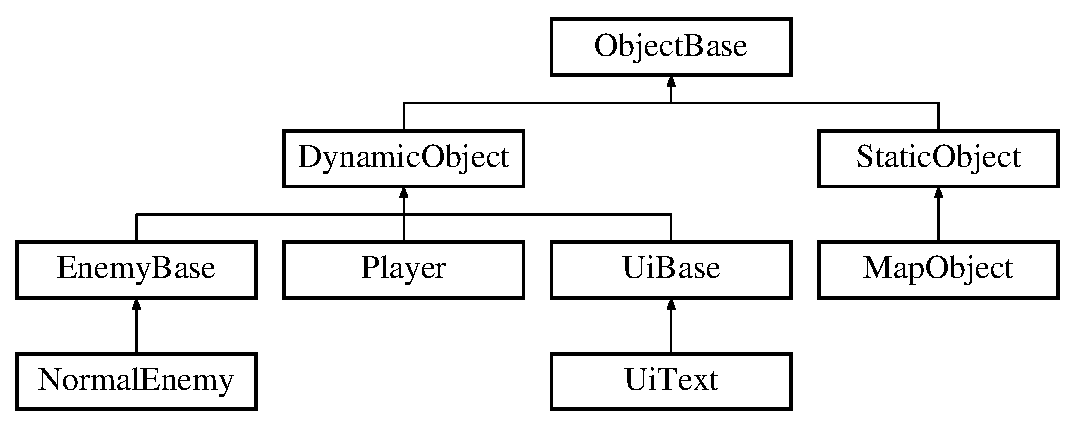
\includegraphics[height=4.000000cm]{class_object_base}
\end{center}
\end{figure}
\subsection*{公開メンバ関数}
\begin{DoxyCompactItemize}
\item 
\mbox{\hyperlink{class_object_base_af2c3a18da2d1cd1c0dd5fae168207f0c}{Object\+Base}} ()
\begin{DoxyCompactList}\small\item\em コンストラクタ \end{DoxyCompactList}\item 
void \mbox{\hyperlink{class_object_base_aea82aedc489b0a9d9990aafa06eef514}{Init}} (std\+::string name, W\+C\+H\+AR $\ast$path, const L\+O\+NG w, const L\+O\+NG h, \mbox{\hyperlink{transform_8h_afb0c5e21d4133ff4f200992c0b534e1b}{V\+E\+C2}} pos, float rot=0, float scale=1, bool all\+\_\+render=true)
\begin{DoxyCompactList}\small\item\em 初期化 \end{DoxyCompactList}\item 
void \mbox{\hyperlink{class_object_base_a5b5672034139b22235ada326eb16dd3e}{Update}} ()
\begin{DoxyCompactList}\small\item\em 更新するかどうか決める \end{DoxyCompactList}\item 
void \mbox{\hyperlink{class_object_base_ac84be5b56d23b8809ca08e27c0dcb16a}{Render}} (bool=true, const \mbox{\hyperlink{class_transform}{Transform}} \&=N\+U\+LL)
\begin{DoxyCompactList}\small\item\em 描画するかどうかを決める \end{DoxyCompactList}\item 
virtual void \mbox{\hyperlink{class_object_base_a7fa4c548153c3af20f89673ffea809af}{Destroy}} ()=0
\item 
virtual \mbox{\hyperlink{class_object_base_a7074bc9389069351c2d0eee6a47e5ee3}{$\sim$\+Object\+Base}} ()
\item 
virtual void \mbox{\hyperlink{class_object_base_a1991d1c2c214a593feb6b6b24802a8c4}{Collision}} (\mbox{\hyperlink{class_object_base}{Object\+Base}} $\ast$)
\end{DoxyCompactItemize}
\subsection*{公開変数類}
\begin{DoxyCompactItemize}
\item 
\mbox{\hyperlink{object__base_8h_a0eff9883ab049ee02773dde19d057c0c}{O\+B\+J\+E\+C\+T\+\_\+\+T\+AG}} \mbox{\hyperlink{class_object_base_aff7eb5482ca9bc1cd30b84994d0dad8b}{object\+\_\+tag}}
\item 
bool \mbox{\hyperlink{class_object_base_ade1c868f20653a6fa5236544120eca2b}{enabled}}
\item 
\mbox{\hyperlink{class_transform}{Transform}} \mbox{\hyperlink{class_object_base_ac8096c26fe09682da6119208d392dc62}{transform}}
\end{DoxyCompactItemize}
\subsection*{限定公開メンバ関数}
\begin{DoxyCompactItemize}
\item 
virtual void \mbox{\hyperlink{class_object_base_af133f36f2bca1dcfd962e2cfac61ab51}{Init\+Process}} ()=0
\item 
virtual void \mbox{\hyperlink{class_object_base_aeac51d868beeb7f7fe900407b76b93a2}{Render\+Process}} (bool)=0
\item 
virtual void \mbox{\hyperlink{class_object_base_a8b5b72b363a419767efde0b0e692ea95}{Update\+Process}} ()=0
\end{DoxyCompactItemize}
\subsection*{限定公開変数類}
\begin{DoxyCompactItemize}
\item 
\mbox{\hyperlink{class_sprite}{Sprite}} \mbox{\hyperlink{class_object_base_a16415e349623e10f45518fb637f7051b}{sprite}}
\item 
\mbox{\hyperlink{class_transform}{Transform}} \mbox{\hyperlink{class_object_base_abedc2ea4baa694611f8822ea6e04b210}{world\+Transform}}
\end{DoxyCompactItemize}


\subsection{詳解}
オブジェクトのスーパークラス 

\subsection{構築子と解体子}
\mbox{\Hypertarget{class_object_base_af2c3a18da2d1cd1c0dd5fae168207f0c}\label{class_object_base_af2c3a18da2d1cd1c0dd5fae168207f0c}} 
\index{Object\+Base@{Object\+Base}!Object\+Base@{Object\+Base}}
\index{Object\+Base@{Object\+Base}!Object\+Base@{Object\+Base}}
\subsubsection{\texorpdfstring{Object\+Base()}{ObjectBase()}}
{\footnotesize\ttfamily Object\+Base\+::\+Object\+Base (\begin{DoxyParamCaption}{ }\end{DoxyParamCaption})\hspace{0.3cm}{\ttfamily [inline]}}



コンストラクタ 

\mbox{\Hypertarget{class_object_base_a7074bc9389069351c2d0eee6a47e5ee3}\label{class_object_base_a7074bc9389069351c2d0eee6a47e5ee3}} 
\index{Object\+Base@{Object\+Base}!````~Object\+Base@{$\sim$\+Object\+Base}}
\index{````~Object\+Base@{$\sim$\+Object\+Base}!Object\+Base@{Object\+Base}}
\subsubsection{\texorpdfstring{$\sim$\+Object\+Base()}{~ObjectBase()}}
{\footnotesize\ttfamily virtual Object\+Base\+::$\sim$\+Object\+Base (\begin{DoxyParamCaption}{ }\end{DoxyParamCaption})\hspace{0.3cm}{\ttfamily [inline]}, {\ttfamily [virtual]}}



\subsection{関数詳解}
\mbox{\Hypertarget{class_object_base_a1991d1c2c214a593feb6b6b24802a8c4}\label{class_object_base_a1991d1c2c214a593feb6b6b24802a8c4}} 
\index{Object\+Base@{Object\+Base}!Collision@{Collision}}
\index{Collision@{Collision}!Object\+Base@{Object\+Base}}
\subsubsection{\texorpdfstring{Collision()}{Collision()}}
{\footnotesize\ttfamily virtual void Object\+Base\+::\+Collision (\begin{DoxyParamCaption}\item[{\mbox{\hyperlink{class_object_base}{Object\+Base}} $\ast$}]{ }\end{DoxyParamCaption})\hspace{0.3cm}{\ttfamily [inline]}, {\ttfamily [virtual]}}



\mbox{\hyperlink{class_player_a660421b69afc7cd6d0d97ea9a28251a2}{Player}}で再実装されています。

\mbox{\Hypertarget{class_object_base_a7fa4c548153c3af20f89673ffea809af}\label{class_object_base_a7fa4c548153c3af20f89673ffea809af}} 
\index{Object\+Base@{Object\+Base}!Destroy@{Destroy}}
\index{Destroy@{Destroy}!Object\+Base@{Object\+Base}}
\subsubsection{\texorpdfstring{Destroy()}{Destroy()}}
{\footnotesize\ttfamily virtual void Object\+Base\+::\+Destroy (\begin{DoxyParamCaption}{ }\end{DoxyParamCaption})\hspace{0.3cm}{\ttfamily [pure virtual]}}



\mbox{\hyperlink{class_player_af2cf4936165ef12cce96f7994e0879df}{Player}}, \mbox{\hyperlink{class_static_object_aac4b963c88ebffb128bcaf5abf09768b}{Static\+Object}}で実装されています。

\mbox{\Hypertarget{class_object_base_aea82aedc489b0a9d9990aafa06eef514}\label{class_object_base_aea82aedc489b0a9d9990aafa06eef514}} 
\index{Object\+Base@{Object\+Base}!Init@{Init}}
\index{Init@{Init}!Object\+Base@{Object\+Base}}
\subsubsection{\texorpdfstring{Init()}{Init()}}
{\footnotesize\ttfamily void Object\+Base\+::\+Init (\begin{DoxyParamCaption}\item[{std\+::string}]{name,  }\item[{W\+C\+H\+AR $\ast$}]{path,  }\item[{const L\+O\+NG}]{w,  }\item[{const L\+O\+NG}]{h,  }\item[{\mbox{\hyperlink{transform_8h_afb0c5e21d4133ff4f200992c0b534e1b}{V\+E\+C2}}}]{pos,  }\item[{float}]{rot = {\ttfamily 0},  }\item[{float}]{scale = {\ttfamily 1},  }\item[{bool}]{all\+\_\+render = {\ttfamily true} }\end{DoxyParamCaption})}



初期化 


\begin{DoxyParams}{引数}
{\em name} & mapで管理するためのキー \\
\hline
{\em path} & テクスチャのパス \\
\hline
{\em w,h} & テクスチャのサイズ \\
\hline
{\em pos} & 初期位置 \\
\hline
{\em rot} & 回転 \\
\hline
{\em scale} & サイズ \\
\hline
{\em テクスチャをすべて描画するかどうか} & \\
\hline
\end{DoxyParams}
\mbox{\Hypertarget{class_object_base_af133f36f2bca1dcfd962e2cfac61ab51}\label{class_object_base_af133f36f2bca1dcfd962e2cfac61ab51}} 
\index{Object\+Base@{Object\+Base}!Init\+Process@{Init\+Process}}
\index{Init\+Process@{Init\+Process}!Object\+Base@{Object\+Base}}
\subsubsection{\texorpdfstring{Init\+Process()}{InitProcess()}}
{\footnotesize\ttfamily virtual void Object\+Base\+::\+Init\+Process (\begin{DoxyParamCaption}{ }\end{DoxyParamCaption})\hspace{0.3cm}{\ttfamily [protected]}, {\ttfamily [pure virtual]}}



\mbox{\hyperlink{class_player_a1051f85c8bf18a256d275d1a1dee5da6}{Player}}, \mbox{\hyperlink{class_static_object_ae9563da84f7045d6206c938963d5aecf}{Static\+Object}}で実装されています。

\mbox{\Hypertarget{class_object_base_ac84be5b56d23b8809ca08e27c0dcb16a}\label{class_object_base_ac84be5b56d23b8809ca08e27c0dcb16a}} 
\index{Object\+Base@{Object\+Base}!Render@{Render}}
\index{Render@{Render}!Object\+Base@{Object\+Base}}
\subsubsection{\texorpdfstring{Render()}{Render()}}
{\footnotesize\ttfamily void Object\+Base\+::\+Render (\begin{DoxyParamCaption}\item[{bool}]{camera\+\_\+affected = {\ttfamily true},  }\item[{const \mbox{\hyperlink{class_transform}{Transform}} \&}]{t = {\ttfamily NULL} }\end{DoxyParamCaption})}



描画するかどうかを決める 

\mbox{\Hypertarget{class_object_base_aeac51d868beeb7f7fe900407b76b93a2}\label{class_object_base_aeac51d868beeb7f7fe900407b76b93a2}} 
\index{Object\+Base@{Object\+Base}!Render\+Process@{Render\+Process}}
\index{Render\+Process@{Render\+Process}!Object\+Base@{Object\+Base}}
\subsubsection{\texorpdfstring{Render\+Process()}{RenderProcess()}}
{\footnotesize\ttfamily virtual void Object\+Base\+::\+Render\+Process (\begin{DoxyParamCaption}\item[{bool}]{ }\end{DoxyParamCaption})\hspace{0.3cm}{\ttfamily [protected]}, {\ttfamily [pure virtual]}}



\mbox{\hyperlink{class_dynamic_object_aa7488e1b4dfd7049447535d93d9d6783}{Dynamic\+Object}}, \mbox{\hyperlink{class_static_object_afec57009537695c4715386120a619942}{Static\+Object}}で実装されています。

\mbox{\Hypertarget{class_object_base_a5b5672034139b22235ada326eb16dd3e}\label{class_object_base_a5b5672034139b22235ada326eb16dd3e}} 
\index{Object\+Base@{Object\+Base}!Update@{Update}}
\index{Update@{Update}!Object\+Base@{Object\+Base}}
\subsubsection{\texorpdfstring{Update()}{Update()}}
{\footnotesize\ttfamily void Object\+Base\+::\+Update (\begin{DoxyParamCaption}{ }\end{DoxyParamCaption})}



更新するかどうか決める 

\mbox{\Hypertarget{class_object_base_a8b5b72b363a419767efde0b0e692ea95}\label{class_object_base_a8b5b72b363a419767efde0b0e692ea95}} 
\index{Object\+Base@{Object\+Base}!Update\+Process@{Update\+Process}}
\index{Update\+Process@{Update\+Process}!Object\+Base@{Object\+Base}}
\subsubsection{\texorpdfstring{Update\+Process()}{UpdateProcess()}}
{\footnotesize\ttfamily virtual void Object\+Base\+::\+Update\+Process (\begin{DoxyParamCaption}{ }\end{DoxyParamCaption})\hspace{0.3cm}{\ttfamily [protected]}, {\ttfamily [pure virtual]}}



\mbox{\hyperlink{class_player_ab8accc9b83b030f5313f1b4872a7e634}{Player}}, \mbox{\hyperlink{class_static_object_a0dd0ec514aa597a1dd83a1168902a079}{Static\+Object}}で実装されています。



\subsection{メンバ詳解}
\mbox{\Hypertarget{class_object_base_ade1c868f20653a6fa5236544120eca2b}\label{class_object_base_ade1c868f20653a6fa5236544120eca2b}} 
\index{Object\+Base@{Object\+Base}!enabled@{enabled}}
\index{enabled@{enabled}!Object\+Base@{Object\+Base}}
\subsubsection{\texorpdfstring{enabled}{enabled}}
{\footnotesize\ttfamily bool Object\+Base\+::enabled}

\mbox{\Hypertarget{class_object_base_aff7eb5482ca9bc1cd30b84994d0dad8b}\label{class_object_base_aff7eb5482ca9bc1cd30b84994d0dad8b}} 
\index{Object\+Base@{Object\+Base}!object\+\_\+tag@{object\+\_\+tag}}
\index{object\+\_\+tag@{object\+\_\+tag}!Object\+Base@{Object\+Base}}
\subsubsection{\texorpdfstring{object\+\_\+tag}{object\_tag}}
{\footnotesize\ttfamily \mbox{\hyperlink{object__base_8h_a0eff9883ab049ee02773dde19d057c0c}{O\+B\+J\+E\+C\+T\+\_\+\+T\+AG}} Object\+Base\+::object\+\_\+tag}

\mbox{\Hypertarget{class_object_base_a16415e349623e10f45518fb637f7051b}\label{class_object_base_a16415e349623e10f45518fb637f7051b}} 
\index{Object\+Base@{Object\+Base}!sprite@{sprite}}
\index{sprite@{sprite}!Object\+Base@{Object\+Base}}
\subsubsection{\texorpdfstring{sprite}{sprite}}
{\footnotesize\ttfamily \mbox{\hyperlink{class_sprite}{Sprite}} Object\+Base\+::sprite\hspace{0.3cm}{\ttfamily [protected]}}

\mbox{\Hypertarget{class_object_base_ac8096c26fe09682da6119208d392dc62}\label{class_object_base_ac8096c26fe09682da6119208d392dc62}} 
\index{Object\+Base@{Object\+Base}!transform@{transform}}
\index{transform@{transform}!Object\+Base@{Object\+Base}}
\subsubsection{\texorpdfstring{transform}{transform}}
{\footnotesize\ttfamily \mbox{\hyperlink{class_transform}{Transform}} Object\+Base\+::transform}

\mbox{\Hypertarget{class_object_base_abedc2ea4baa694611f8822ea6e04b210}\label{class_object_base_abedc2ea4baa694611f8822ea6e04b210}} 
\index{Object\+Base@{Object\+Base}!world\+Transform@{world\+Transform}}
\index{world\+Transform@{world\+Transform}!Object\+Base@{Object\+Base}}
\subsubsection{\texorpdfstring{world\+Transform}{worldTransform}}
{\footnotesize\ttfamily \mbox{\hyperlink{class_transform}{Transform}} Object\+Base\+::world\+Transform\hspace{0.3cm}{\ttfamily [protected]}}



このクラス詳解は次のファイルから抽出されました\+:\begin{DoxyCompactItemize}
\item 
C\+:/\+Users/tokir/\+Documents/\+Git\+Hub/\+Weapon\+Merchant\+Adventure/src/object/base/\mbox{\hyperlink{object__base_8h}{object\+\_\+base.\+h}}\item 
C\+:/\+Users/tokir/\+Documents/\+Git\+Hub/\+Weapon\+Merchant\+Adventure/src/object/base/\mbox{\hyperlink{object__base_8cpp}{object\+\_\+base.\+cpp}}\end{DoxyCompactItemize}

\hypertarget{class_player}{}\section{Player クラス}
\label{class_player}\index{Player@{Player}}


プレイヤークラス  




{\ttfamily \#include $<$player.\+h$>$}

Player の継承関係図\begin{figure}[H]
\begin{center}
\leavevmode
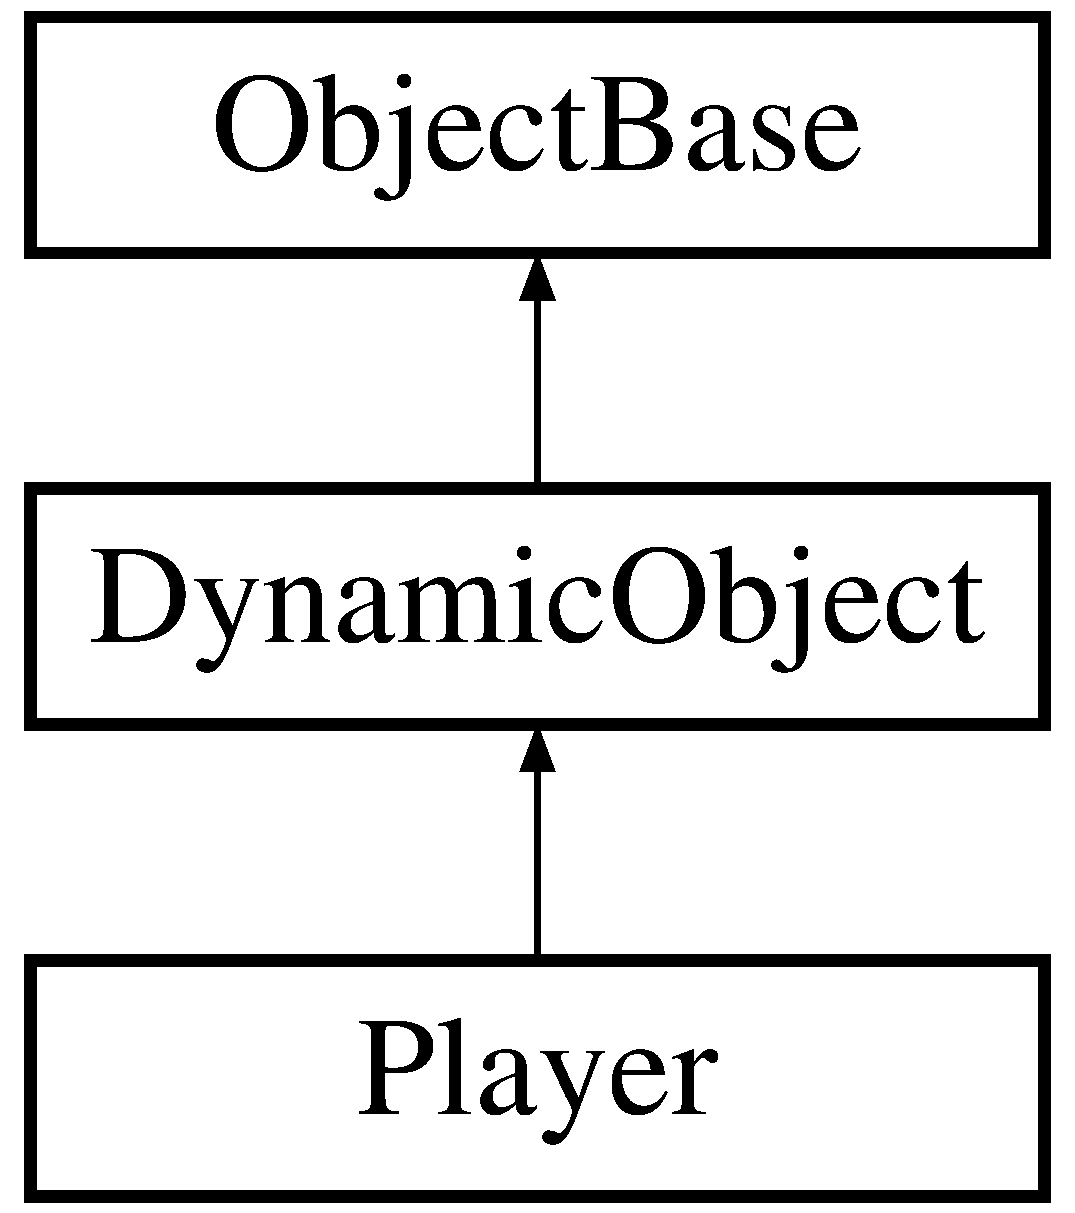
\includegraphics[height=3.000000cm]{class_player}
\end{center}
\end{figure}
\subsection*{公開メンバ関数}
\begin{DoxyCompactItemize}
\item 
void \mbox{\hyperlink{class_player_a848c2ecb62431010eaa9298b2c2c4be0}{Ui\+Render}} ()
\begin{DoxyCompactList}\small\item\em U\+Iの描画 \end{DoxyCompactList}\item 
void \mbox{\hyperlink{class_player_a615af41886fe293fcc3c6f276de77991}{Enabled\+Weapon}} ()
\begin{DoxyCompactList}\small\item\em 武器の非表示 \end{DoxyCompactList}\item 
void \mbox{\hyperlink{class_player_a97012a8b2bead252582ff39e852961ac}{Eenabled\+True\+Weapon}} ()
\begin{DoxyCompactList}\small\item\em 武器の表示 \end{DoxyCompactList}\item 
void \mbox{\hyperlink{class_player_a662de093359fb8e4a5bdc86a34fd2549}{Translation\+Boss\+Scene}} ()
\begin{DoxyCompactList}\small\item\em ボスシーンに移行するときの処理 \end{DoxyCompactList}\item 
void \mbox{\hyperlink{class_player_aff4d2bffe97e2b70f47f5eac2da26562}{In\+Boss\+Scene}} ()
\begin{DoxyCompactList}\small\item\em ボスシーンに入ったときの処理 \end{DoxyCompactList}\item 
void \mbox{\hyperlink{class_player_af1b9f4482efa53508befe6de204a3da6}{Animation\+Walk}} (bool right)
\begin{DoxyCompactList}\small\item\em 歩くアニメーションのみ関数化 \end{DoxyCompactList}\item 
void \mbox{\hyperlink{class_player_a8b27da2bdfb3e25337c7b6fd345d21f2}{Clear\+Update}} ()
\begin{DoxyCompactList}\small\item\em クリアした時の更新 \end{DoxyCompactList}\item 
void \mbox{\hyperlink{class_player_a6ddf26051788b56dd4029ba851e1f35a}{Reset\+Speed}} ()
\begin{DoxyCompactList}\small\item\em 横方向の力を0にする \end{DoxyCompactList}\item 
void \mbox{\hyperlink{class_player_af2cf4936165ef12cce96f7994e0879df}{Destroy}} () final
\begin{DoxyCompactList}\small\item\em プレイヤーの破棄 \end{DoxyCompactList}\item 
void \mbox{\hyperlink{class_player_abbb6662f1dc4ba3f75cafa6100160da0}{Update\+Animation}} (bool right=true)
\begin{DoxyCompactList}\small\item\em アニメーションの更新 \end{DoxyCompactList}\item 
\mbox{\hyperlink{class_player_affe0cc3cb714f6deb4e62f0c0d3f1fd8}{Player}} ()
\begin{DoxyCompactList}\small\item\em コンストラクタ \end{DoxyCompactList}\item 
\mbox{\hyperlink{class_player_a635af5e438af5a296c88f768e5e93eb0}{Player}} (\mbox{\hyperlink{class_player}{Player}} \&\&other) noexcept
\begin{DoxyCompactList}\small\item\em ムーブコンストラクタ \end{DoxyCompactList}\item 
\mbox{\hyperlink{class_player}{Player}} \& \mbox{\hyperlink{class_player_a8868988ae751daed5cfa32627e78889b}{operator=}} (const \mbox{\hyperlink{class_player}{Player}} \&other)
\begin{DoxyCompactList}\small\item\em コピー代入演算子 \end{DoxyCompactList}\item 
void \mbox{\hyperlink{class_player_a992b5c7e0d981308ed56706c6e71a709}{Collision}} (\mbox{\hyperlink{class_object_base}{Object\+Base}} $\ast$, \mbox{\hyperlink{common_8h_ae148fff5818e9444b4ab2288829559bf}{Vec2}}) final
\begin{DoxyCompactList}\small\item\em 当たってるときに実行する関数 \end{DoxyCompactList}\item 
void \mbox{\hyperlink{class_player_a6c879db24d39d894207e078eb4c56e8d}{Attack}} ()
\begin{DoxyCompactList}\small\item\em 攻撃 \end{DoxyCompactList}\end{DoxyCompactItemize}
\subsection*{公開変数類}
\begin{DoxyCompactItemize}
\item 
bool \mbox{\hyperlink{class_player_adf34c7a3a58c3f8e7f7201ed962a03f0}{boss\+\_\+scene}} = false
\end{DoxyCompactItemize}
\subsection*{限定公開メンバ関数}
\begin{DoxyCompactItemize}
\item 
void \mbox{\hyperlink{class_player_a1051f85c8bf18a256d275d1a1dee5da6}{Init\+Process}} () final
\begin{DoxyCompactList}\small\item\em 初期化 \end{DoxyCompactList}\item 
void \mbox{\hyperlink{class_player_ab8accc9b83b030f5313f1b4872a7e634}{Update\+Process}} () final
\begin{DoxyCompactList}\small\item\em プレイヤーの更新 \end{DoxyCompactList}\item 
void \mbox{\hyperlink{class_player_a8ac2e54fe5672d32186456b9735c02c3}{Render\+Process}} (bool camera\+\_\+affected) final
\begin{DoxyCompactList}\small\item\em プレイヤーの描画 \end{DoxyCompactList}\end{DoxyCompactItemize}
\subsection*{その他の継承メンバ}


\subsection{詳解}
プレイヤークラス 

\subsection{構築子と解体子}
\mbox{\Hypertarget{class_player_affe0cc3cb714f6deb4e62f0c0d3f1fd8}\label{class_player_affe0cc3cb714f6deb4e62f0c0d3f1fd8}} 
\index{Player@{Player}!Player@{Player}}
\index{Player@{Player}!Player@{Player}}
\subsubsection{\texorpdfstring{Player()}{Player()}\hspace{0.1cm}{\footnotesize\ttfamily [1/2]}}
{\footnotesize\ttfamily Player\+::\+Player (\begin{DoxyParamCaption}{ }\end{DoxyParamCaption})\hspace{0.3cm}{\ttfamily [inline]}}



コンストラクタ 

\mbox{\Hypertarget{class_player_a635af5e438af5a296c88f768e5e93eb0}\label{class_player_a635af5e438af5a296c88f768e5e93eb0}} 
\index{Player@{Player}!Player@{Player}}
\index{Player@{Player}!Player@{Player}}
\subsubsection{\texorpdfstring{Player()}{Player()}\hspace{0.1cm}{\footnotesize\ttfamily [2/2]}}
{\footnotesize\ttfamily Player\+::\+Player (\begin{DoxyParamCaption}\item[{\mbox{\hyperlink{class_player}{Player}} \&\&}]{other }\end{DoxyParamCaption})\hspace{0.3cm}{\ttfamily [inline]}, {\ttfamily [noexcept]}}



ムーブコンストラクタ 



\subsection{関数詳解}
\mbox{\Hypertarget{class_player_af1b9f4482efa53508befe6de204a3da6}\label{class_player_af1b9f4482efa53508befe6de204a3da6}} 
\index{Player@{Player}!Animation\+Walk@{Animation\+Walk}}
\index{Animation\+Walk@{Animation\+Walk}!Player@{Player}}
\subsubsection{\texorpdfstring{Animation\+Walk()}{AnimationWalk()}}
{\footnotesize\ttfamily void Player\+::\+Animation\+Walk (\begin{DoxyParamCaption}\item[{bool}]{right }\end{DoxyParamCaption})\hspace{0.3cm}{\ttfamily [inline]}}



歩くアニメーションのみ関数化 


\begin{DoxyParams}{引数}
{\em right} & 右かどうか \\
\hline
\end{DoxyParams}
\mbox{\Hypertarget{class_player_a6c879db24d39d894207e078eb4c56e8d}\label{class_player_a6c879db24d39d894207e078eb4c56e8d}} 
\index{Player@{Player}!Attack@{Attack}}
\index{Attack@{Attack}!Player@{Player}}
\subsubsection{\texorpdfstring{Attack()}{Attack()}}
{\footnotesize\ttfamily void Player\+::\+Attack (\begin{DoxyParamCaption}{ }\end{DoxyParamCaption})}



攻撃 

\mbox{\Hypertarget{class_player_a8b27da2bdfb3e25337c7b6fd345d21f2}\label{class_player_a8b27da2bdfb3e25337c7b6fd345d21f2}} 
\index{Player@{Player}!Clear\+Update@{Clear\+Update}}
\index{Clear\+Update@{Clear\+Update}!Player@{Player}}
\subsubsection{\texorpdfstring{Clear\+Update()}{ClearUpdate()}}
{\footnotesize\ttfamily void Player\+::\+Clear\+Update (\begin{DoxyParamCaption}{ }\end{DoxyParamCaption})\hspace{0.3cm}{\ttfamily [inline]}}



クリアした時の更新 

\mbox{\Hypertarget{class_player_a992b5c7e0d981308ed56706c6e71a709}\label{class_player_a992b5c7e0d981308ed56706c6e71a709}} 
\index{Player@{Player}!Collision@{Collision}}
\index{Collision@{Collision}!Player@{Player}}
\subsubsection{\texorpdfstring{Collision()}{Collision()}}
{\footnotesize\ttfamily void Player\+::\+Collision (\begin{DoxyParamCaption}\item[{\mbox{\hyperlink{class_object_base}{Object\+Base}} $\ast$}]{obj,  }\item[{\mbox{\hyperlink{common_8h_ae148fff5818e9444b4ab2288829559bf}{Vec2}}}]{ }\end{DoxyParamCaption})\hspace{0.3cm}{\ttfamily [final]}, {\ttfamily [virtual]}}



当たってるときに実行する関数 



\mbox{\hyperlink{class_object_base_a3e1db79dfa119be067d816c22d09839d}{Object\+Base}}を再実装しています。

\mbox{\Hypertarget{class_player_af2cf4936165ef12cce96f7994e0879df}\label{class_player_af2cf4936165ef12cce96f7994e0879df}} 
\index{Player@{Player}!Destroy@{Destroy}}
\index{Destroy@{Destroy}!Player@{Player}}
\subsubsection{\texorpdfstring{Destroy()}{Destroy()}}
{\footnotesize\ttfamily void Player\+::\+Destroy (\begin{DoxyParamCaption}{ }\end{DoxyParamCaption})\hspace{0.3cm}{\ttfamily [final]}, {\ttfamily [virtual]}}



プレイヤーの破棄 



\mbox{\hyperlink{class_object_base_a7fa4c548153c3af20f89673ffea809af}{Object\+Base}}を実装しています。

\mbox{\Hypertarget{class_player_a97012a8b2bead252582ff39e852961ac}\label{class_player_a97012a8b2bead252582ff39e852961ac}} 
\index{Player@{Player}!Eenabled\+True\+Weapon@{Eenabled\+True\+Weapon}}
\index{Eenabled\+True\+Weapon@{Eenabled\+True\+Weapon}!Player@{Player}}
\subsubsection{\texorpdfstring{Eenabled\+True\+Weapon()}{EenabledTrueWeapon()}}
{\footnotesize\ttfamily void Player\+::\+Eenabled\+True\+Weapon (\begin{DoxyParamCaption}{ }\end{DoxyParamCaption})\hspace{0.3cm}{\ttfamily [inline]}}



武器の表示 

\mbox{\Hypertarget{class_player_a615af41886fe293fcc3c6f276de77991}\label{class_player_a615af41886fe293fcc3c6f276de77991}} 
\index{Player@{Player}!Enabled\+Weapon@{Enabled\+Weapon}}
\index{Enabled\+Weapon@{Enabled\+Weapon}!Player@{Player}}
\subsubsection{\texorpdfstring{Enabled\+Weapon()}{EnabledWeapon()}}
{\footnotesize\ttfamily void Player\+::\+Enabled\+Weapon (\begin{DoxyParamCaption}{ }\end{DoxyParamCaption})\hspace{0.3cm}{\ttfamily [inline]}}



武器の非表示 

\mbox{\Hypertarget{class_player_aff4d2bffe97e2b70f47f5eac2da26562}\label{class_player_aff4d2bffe97e2b70f47f5eac2da26562}} 
\index{Player@{Player}!In\+Boss\+Scene@{In\+Boss\+Scene}}
\index{In\+Boss\+Scene@{In\+Boss\+Scene}!Player@{Player}}
\subsubsection{\texorpdfstring{In\+Boss\+Scene()}{InBossScene()}}
{\footnotesize\ttfamily void Player\+::\+In\+Boss\+Scene (\begin{DoxyParamCaption}{ }\end{DoxyParamCaption})\hspace{0.3cm}{\ttfamily [inline]}}



ボスシーンに入ったときの処理 

\mbox{\Hypertarget{class_player_a1051f85c8bf18a256d275d1a1dee5da6}\label{class_player_a1051f85c8bf18a256d275d1a1dee5da6}} 
\index{Player@{Player}!Init\+Process@{Init\+Process}}
\index{Init\+Process@{Init\+Process}!Player@{Player}}
\subsubsection{\texorpdfstring{Init\+Process()}{InitProcess()}}
{\footnotesize\ttfamily void Player\+::\+Init\+Process (\begin{DoxyParamCaption}{ }\end{DoxyParamCaption})\hspace{0.3cm}{\ttfamily [final]}, {\ttfamily [protected]}, {\ttfamily [virtual]}}



初期化 



\mbox{\hyperlink{class_object_base_af133f36f2bca1dcfd962e2cfac61ab51}{Object\+Base}}を実装しています。

\mbox{\Hypertarget{class_player_a8868988ae751daed5cfa32627e78889b}\label{class_player_a8868988ae751daed5cfa32627e78889b}} 
\index{Player@{Player}!operator=@{operator=}}
\index{operator=@{operator=}!Player@{Player}}
\subsubsection{\texorpdfstring{operator=()}{operator=()}}
{\footnotesize\ttfamily \mbox{\hyperlink{class_player}{Player}}\& Player\+::operator= (\begin{DoxyParamCaption}\item[{const \mbox{\hyperlink{class_player}{Player}} \&}]{other }\end{DoxyParamCaption})\hspace{0.3cm}{\ttfamily [inline]}}



コピー代入演算子 

\mbox{\Hypertarget{class_player_a8ac2e54fe5672d32186456b9735c02c3}\label{class_player_a8ac2e54fe5672d32186456b9735c02c3}} 
\index{Player@{Player}!Render\+Process@{Render\+Process}}
\index{Render\+Process@{Render\+Process}!Player@{Player}}
\subsubsection{\texorpdfstring{Render\+Process()}{RenderProcess()}}
{\footnotesize\ttfamily void Player\+::\+Render\+Process (\begin{DoxyParamCaption}\item[{bool}]{camera\+\_\+affected }\end{DoxyParamCaption})\hspace{0.3cm}{\ttfamily [final]}, {\ttfamily [protected]}, {\ttfamily [virtual]}}



プレイヤーの描画 


\begin{DoxyParams}{引数}
{\em camera\+\_\+affected} & カメラの位置によって描画する位置を変えるかどうか \\
\hline
\end{DoxyParams}


\mbox{\hyperlink{class_dynamic_object_aa7488e1b4dfd7049447535d93d9d6783}{Dynamic\+Object}}を再実装しています。

\mbox{\Hypertarget{class_player_a6ddf26051788b56dd4029ba851e1f35a}\label{class_player_a6ddf26051788b56dd4029ba851e1f35a}} 
\index{Player@{Player}!Reset\+Speed@{Reset\+Speed}}
\index{Reset\+Speed@{Reset\+Speed}!Player@{Player}}
\subsubsection{\texorpdfstring{Reset\+Speed()}{ResetSpeed()}}
{\footnotesize\ttfamily void Player\+::\+Reset\+Speed (\begin{DoxyParamCaption}{ }\end{DoxyParamCaption})\hspace{0.3cm}{\ttfamily [inline]}}



横方向の力を0にする 

\mbox{\Hypertarget{class_player_a662de093359fb8e4a5bdc86a34fd2549}\label{class_player_a662de093359fb8e4a5bdc86a34fd2549}} 
\index{Player@{Player}!Translation\+Boss\+Scene@{Translation\+Boss\+Scene}}
\index{Translation\+Boss\+Scene@{Translation\+Boss\+Scene}!Player@{Player}}
\subsubsection{\texorpdfstring{Translation\+Boss\+Scene()}{TranslationBossScene()}}
{\footnotesize\ttfamily void Player\+::\+Translation\+Boss\+Scene (\begin{DoxyParamCaption}{ }\end{DoxyParamCaption})\hspace{0.3cm}{\ttfamily [inline]}}



ボスシーンに移行するときの処理 

\mbox{\Hypertarget{class_player_a848c2ecb62431010eaa9298b2c2c4be0}\label{class_player_a848c2ecb62431010eaa9298b2c2c4be0}} 
\index{Player@{Player}!Ui\+Render@{Ui\+Render}}
\index{Ui\+Render@{Ui\+Render}!Player@{Player}}
\subsubsection{\texorpdfstring{Ui\+Render()}{UiRender()}}
{\footnotesize\ttfamily void Player\+::\+Ui\+Render (\begin{DoxyParamCaption}{ }\end{DoxyParamCaption})}



U\+Iの描画 

\mbox{\Hypertarget{class_player_abbb6662f1dc4ba3f75cafa6100160da0}\label{class_player_abbb6662f1dc4ba3f75cafa6100160da0}} 
\index{Player@{Player}!Update\+Animation@{Update\+Animation}}
\index{Update\+Animation@{Update\+Animation}!Player@{Player}}
\subsubsection{\texorpdfstring{Update\+Animation()}{UpdateAnimation()}}
{\footnotesize\ttfamily void Player\+::\+Update\+Animation (\begin{DoxyParamCaption}\item[{bool}]{right = {\ttfamily true} }\end{DoxyParamCaption})\hspace{0.3cm}{\ttfamily [inline]}}



アニメーションの更新 

\mbox{\Hypertarget{class_player_ab8accc9b83b030f5313f1b4872a7e634}\label{class_player_ab8accc9b83b030f5313f1b4872a7e634}} 
\index{Player@{Player}!Update\+Process@{Update\+Process}}
\index{Update\+Process@{Update\+Process}!Player@{Player}}
\subsubsection{\texorpdfstring{Update\+Process()}{UpdateProcess()}}
{\footnotesize\ttfamily void Player\+::\+Update\+Process (\begin{DoxyParamCaption}{ }\end{DoxyParamCaption})\hspace{0.3cm}{\ttfamily [final]}, {\ttfamily [protected]}, {\ttfamily [virtual]}}



プレイヤーの更新 



\mbox{\hyperlink{class_object_base_a8b5b72b363a419767efde0b0e692ea95}{Object\+Base}}を実装しています。



\subsection{メンバ詳解}
\mbox{\Hypertarget{class_player_adf34c7a3a58c3f8e7f7201ed962a03f0}\label{class_player_adf34c7a3a58c3f8e7f7201ed962a03f0}} 
\index{Player@{Player}!boss\+\_\+scene@{boss\+\_\+scene}}
\index{boss\+\_\+scene@{boss\+\_\+scene}!Player@{Player}}
\subsubsection{\texorpdfstring{boss\+\_\+scene}{boss\_scene}}
{\footnotesize\ttfamily bool Player\+::boss\+\_\+scene = false}



このクラス詳解は次のファイルから抽出されました\+:\begin{DoxyCompactItemize}
\item 
C\+:/\+Users/tokir/\+Documents/\+Git\+Hub/\+Weapon\+Merchant\+Adventure/src/src/object/character/player/\mbox{\hyperlink{player_8h}{player.\+h}}\item 
C\+:/\+Users/tokir/\+Documents/\+Git\+Hub/\+Weapon\+Merchant\+Adventure/src/src/object/character/player/\mbox{\hyperlink{player_8cpp}{player.\+cpp}}\end{DoxyCompactItemize}

\hypertarget{class_scene}{}\section{Scene クラス}
\label{class_scene}\index{Scene@{Scene}}


マネージャーを含まないシーンのスーパークラス  




{\ttfamily \#include $<$scene.\+h$>$}

Scene の継承関係図\begin{figure}[H]
\begin{center}
\leavevmode
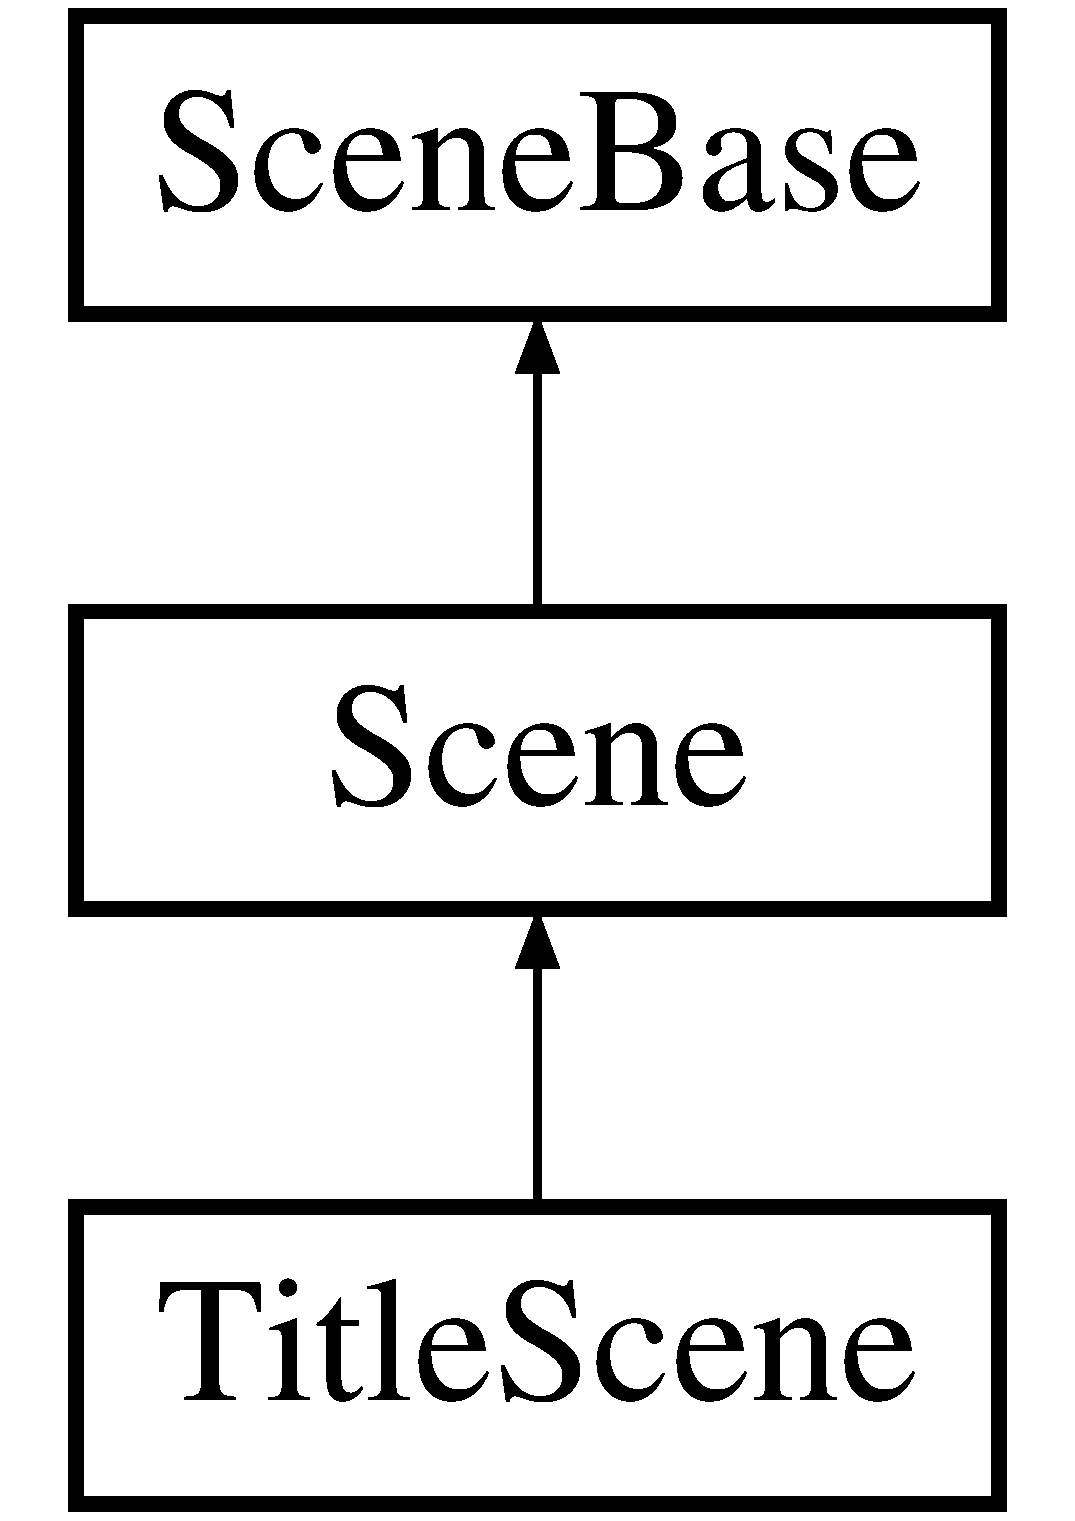
\includegraphics[height=1.875000cm]{class_scene}
\end{center}
\end{figure}
\subsection*{公開メンバ関数}
\begin{DoxyCompactItemize}
\item 
virtual \mbox{\hyperlink{class_scene_aa0a5be58e2ee2d1fdafc5fb46b5e661e}{$\sim$\+Scene}} ()
\item 
virtual std\+::shared\+\_\+ptr$<$ \mbox{\hyperlink{class_scene}{Scene}} $>$ \mbox{\hyperlink{class_scene_ab71ee5f19764b90c87b4574aa1cb1d25}{Update}} (std\+::shared\+\_\+ptr$<$ \mbox{\hyperlink{class_scene}{Scene}} $>$ \&)=0
\item 
virtual void \mbox{\hyperlink{class_scene_ad19a449c6ed452823dae14183689570c}{Exit\+Fade\+Update}} ()
\begin{DoxyCompactList}\small\item\em シーンが変わるときの更新 \end{DoxyCompactList}\end{DoxyCompactItemize}


\subsection{詳解}
マネージャーを含まないシーンのスーパークラス 

マネージャーはこのクラスを保持する 

\subsection{構築子と解体子}
\mbox{\Hypertarget{class_scene_aa0a5be58e2ee2d1fdafc5fb46b5e661e}\label{class_scene_aa0a5be58e2ee2d1fdafc5fb46b5e661e}} 
\index{Scene@{Scene}!````~Scene@{$\sim$\+Scene}}
\index{````~Scene@{$\sim$\+Scene}!Scene@{Scene}}
\subsubsection{\texorpdfstring{$\sim$\+Scene()}{~Scene()}}
{\footnotesize\ttfamily virtual Scene\+::$\sim$\+Scene (\begin{DoxyParamCaption}{ }\end{DoxyParamCaption})\hspace{0.3cm}{\ttfamily [inline]}, {\ttfamily [virtual]}}



\subsection{関数詳解}
\mbox{\Hypertarget{class_scene_ad19a449c6ed452823dae14183689570c}\label{class_scene_ad19a449c6ed452823dae14183689570c}} 
\index{Scene@{Scene}!Exit\+Fade\+Update@{Exit\+Fade\+Update}}
\index{Exit\+Fade\+Update@{Exit\+Fade\+Update}!Scene@{Scene}}
\subsubsection{\texorpdfstring{Exit\+Fade\+Update()}{ExitFadeUpdate()}}
{\footnotesize\ttfamily virtual void Scene\+::\+Exit\+Fade\+Update (\begin{DoxyParamCaption}{ }\end{DoxyParamCaption})\hspace{0.3cm}{\ttfamily [inline]}, {\ttfamily [virtual]}}



シーンが変わるときの更新 



\mbox{\hyperlink{class_select_scene_a546190bc143f6d7a3055935f97b55596}{Select\+Scene}}で再実装されています。

\mbox{\Hypertarget{class_scene_ab71ee5f19764b90c87b4574aa1cb1d25}\label{class_scene_ab71ee5f19764b90c87b4574aa1cb1d25}} 
\index{Scene@{Scene}!Update@{Update}}
\index{Update@{Update}!Scene@{Scene}}
\subsubsection{\texorpdfstring{Update()}{Update()}}
{\footnotesize\ttfamily virtual std\+::shared\+\_\+ptr$<$\mbox{\hyperlink{class_scene}{Scene}}$>$ Scene\+::\+Update (\begin{DoxyParamCaption}\item[{std\+::shared\+\_\+ptr$<$ \mbox{\hyperlink{class_scene}{Scene}} $>$ \&}]{ }\end{DoxyParamCaption})\hspace{0.3cm}{\ttfamily [pure virtual]}}



\mbox{\hyperlink{class_select_scene_a0cef696ddf74155e061cc5f9f2e06419}{Select\+Scene}}, \mbox{\hyperlink{class_title_scene_ab3097e96e2fe65d6fad0d6bb45a14f9f}{Title\+Scene}}, \mbox{\hyperlink{class_pause_scene_a6adfe0685eb6bc64e658f6364c9f704d}{Pause\+Scene}}, \mbox{\hyperlink{class_game_scene_easy_ac2bccbf61722010fd6f317693ee7b8b1}{Game\+Scene\+Easy}}, \mbox{\hyperlink{class_game_scene_hard_ac132a0e281a7d4e6b71deb6e5bcfdb9d}{Game\+Scene\+Hard}}, \mbox{\hyperlink{class_game_scene_normal_a3e45ac3882f1d0dd5c77ab4f0a1ccb33}{Game\+Scene\+Normal}}, \mbox{\hyperlink{class_exit_scene_a18655f3124150a911f266e66e3fc4480}{Exit\+Scene}}で実装されています。



このクラス詳解は次のファイルから抽出されました\+:\begin{DoxyCompactItemize}
\item 
C\+:/\+Users/tokir/\+Documents/\+Git\+Hub/\+Weapon\+Merchant\+Adventure/src/src/scene/\mbox{\hyperlink{scene_8h}{scene.\+h}}\end{DoxyCompactItemize}

\hypertarget{class_scene_base}{}\section{Scene\+Base クラス}
\label{class_scene_base}\index{Scene\+Base@{Scene\+Base}}


マネージャーを含むシーンのスーパークラス  




{\ttfamily \#include $<$scene\+\_\+base.\+h$>$}

Scene\+Base の継承関係図\begin{figure}[H]
\begin{center}
\leavevmode
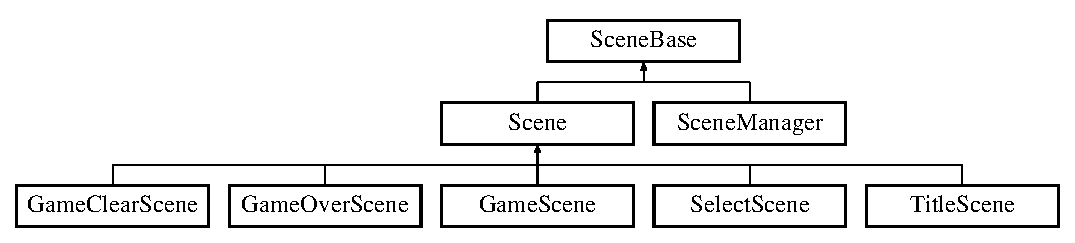
\includegraphics[height=3.000000cm]{class_scene_base}
\end{center}
\end{figure}
\subsection*{公開メンバ関数}
\begin{DoxyCompactItemize}
\item 
virtual \mbox{\hyperlink{class_scene_base_a187dd160e5a16909bcc6529851e38318}{$\sim$\+Scene\+Base}} ()
\item 
virtual void \mbox{\hyperlink{class_scene_base_a24d7db43c819924dc8b07b436f6d3148}{Init}} ()=0
\item 
virtual void \mbox{\hyperlink{class_scene_base_ad981674ce731ea267f398e889bbb9dc3}{Render}} ()=0
\item 
virtual void \mbox{\hyperlink{class_scene_base_a7c5b54020bc519b4dadfe9770d6b27f7}{Destroy}} ()=0
\end{DoxyCompactItemize}
\subsection*{限定公開変数類}
\begin{DoxyCompactItemize}
\item 
\mbox{\hyperlink{scene__base_8h_a24cee5343fb9d0706ead6e8601f363be}{S\+C\+E\+NE}} \mbox{\hyperlink{class_scene_base_a18dcdbacfbd98f73099c3cbeb70ae3b8}{my\+\_\+scene}}
\end{DoxyCompactItemize}


\subsection{詳解}
マネージャーを含むシーンのスーパークラス 

\subsection{構築子と解体子}
\mbox{\Hypertarget{class_scene_base_a187dd160e5a16909bcc6529851e38318}\label{class_scene_base_a187dd160e5a16909bcc6529851e38318}} 
\index{Scene\+Base@{Scene\+Base}!````~Scene\+Base@{$\sim$\+Scene\+Base}}
\index{````~Scene\+Base@{$\sim$\+Scene\+Base}!Scene\+Base@{Scene\+Base}}
\subsubsection{\texorpdfstring{$\sim$\+Scene\+Base()}{~SceneBase()}}
{\footnotesize\ttfamily virtual Scene\+Base\+::$\sim$\+Scene\+Base (\begin{DoxyParamCaption}{ }\end{DoxyParamCaption})\hspace{0.3cm}{\ttfamily [inline]}, {\ttfamily [virtual]}}



\subsection{関数詳解}
\mbox{\Hypertarget{class_scene_base_a7c5b54020bc519b4dadfe9770d6b27f7}\label{class_scene_base_a7c5b54020bc519b4dadfe9770d6b27f7}} 
\index{Scene\+Base@{Scene\+Base}!Destroy@{Destroy}}
\index{Destroy@{Destroy}!Scene\+Base@{Scene\+Base}}
\subsubsection{\texorpdfstring{Destroy()}{Destroy()}}
{\footnotesize\ttfamily virtual void Scene\+Base\+::\+Destroy (\begin{DoxyParamCaption}{ }\end{DoxyParamCaption})\hspace{0.3cm}{\ttfamily [pure virtual]}}



\mbox{\hyperlink{class_title_scene_adfbc5f934572ede2e36419b089c88fe8}{Title\+Scene}}, \mbox{\hyperlink{class_scene_manager_a0e3ad11342e763f0d4108c0b4674a157}{Scene\+Manager}}で実装されています。

\mbox{\Hypertarget{class_scene_base_a24d7db43c819924dc8b07b436f6d3148}\label{class_scene_base_a24d7db43c819924dc8b07b436f6d3148}} 
\index{Scene\+Base@{Scene\+Base}!Init@{Init}}
\index{Init@{Init}!Scene\+Base@{Scene\+Base}}
\subsubsection{\texorpdfstring{Init()}{Init()}}
{\footnotesize\ttfamily virtual void Scene\+Base\+::\+Init (\begin{DoxyParamCaption}{ }\end{DoxyParamCaption})\hspace{0.3cm}{\ttfamily [pure virtual]}}



\mbox{\hyperlink{class_title_scene_a3d039e7db0fa1e22e8c36d3cedfbd318}{Title\+Scene}}, \mbox{\hyperlink{class_scene_manager_a6c0e84d0e76f23fb3172839dba5f091b}{Scene\+Manager}}で実装されています。

\mbox{\Hypertarget{class_scene_base_ad981674ce731ea267f398e889bbb9dc3}\label{class_scene_base_ad981674ce731ea267f398e889bbb9dc3}} 
\index{Scene\+Base@{Scene\+Base}!Render@{Render}}
\index{Render@{Render}!Scene\+Base@{Scene\+Base}}
\subsubsection{\texorpdfstring{Render()}{Render()}}
{\footnotesize\ttfamily virtual void Scene\+Base\+::\+Render (\begin{DoxyParamCaption}{ }\end{DoxyParamCaption})\hspace{0.3cm}{\ttfamily [pure virtual]}}



\mbox{\hyperlink{class_title_scene_af12c59b3bf9458640938c5ca620527ae}{Title\+Scene}}, \mbox{\hyperlink{class_scene_manager_a968ae7a0065b793f139bda6bcc58d106}{Scene\+Manager}}で実装されています。



\subsection{メンバ詳解}
\mbox{\Hypertarget{class_scene_base_a18dcdbacfbd98f73099c3cbeb70ae3b8}\label{class_scene_base_a18dcdbacfbd98f73099c3cbeb70ae3b8}} 
\index{Scene\+Base@{Scene\+Base}!my\+\_\+scene@{my\+\_\+scene}}
\index{my\+\_\+scene@{my\+\_\+scene}!Scene\+Base@{Scene\+Base}}
\subsubsection{\texorpdfstring{my\+\_\+scene}{my\_scene}}
{\footnotesize\ttfamily \mbox{\hyperlink{scene__base_8h_a24cee5343fb9d0706ead6e8601f363be}{S\+C\+E\+NE}} Scene\+Base\+::my\+\_\+scene\hspace{0.3cm}{\ttfamily [protected]}}



このクラス詳解は次のファイルから抽出されました\+:\begin{DoxyCompactItemize}
\item 
C\+:/\+Users/tokir/\+Documents/\+Git\+Hub/\+Weapon\+Merchant\+Adventure/src/scene/base/\mbox{\hyperlink{scene__base_8h}{scene\+\_\+base.\+h}}\end{DoxyCompactItemize}

\hypertarget{class_scene_manager}{}\section{Scene\+Manager クラス}
\label{class_scene_manager}\index{Scene\+Manager@{Scene\+Manager}}


シーンをマネージャーするクラス  




{\ttfamily \#include $<$scene\+\_\+manager.\+h$>$}

Scene\+Manager の継承関係図\begin{figure}[H]
\begin{center}
\leavevmode
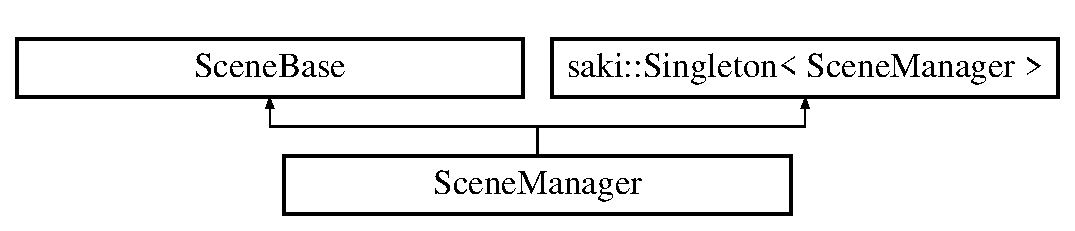
\includegraphics[height=2.000000cm]{class_scene_manager}
\end{center}
\end{figure}
\subsection*{公開メンバ関数}
\begin{DoxyCompactItemize}
\item 
void \mbox{\hyperlink{class_scene_manager_a6c0e84d0e76f23fb3172839dba5f091b}{Init}} () final
\begin{DoxyCompactList}\small\item\em シーンマネージャーの初期化 \end{DoxyCompactList}\item 
void \mbox{\hyperlink{class_scene_manager_a63dcf65832d6a2c190bf496d9a3b00a3}{Update}} ()
\begin{DoxyCompactList}\small\item\em 保持してるシーンの更新 \end{DoxyCompactList}\item 
void \mbox{\hyperlink{class_scene_manager_a968ae7a0065b793f139bda6bcc58d106}{Render}} () final
\begin{DoxyCompactList}\small\item\em 保持してるシーンの描画 \end{DoxyCompactList}\item 
void \mbox{\hyperlink{class_scene_manager_a0e3ad11342e763f0d4108c0b4674a157}{Destroy}} () final
\begin{DoxyCompactList}\small\item\em 保持してるシーンのマネージャーの破棄 \end{DoxyCompactList}\item 
void \mbox{\hyperlink{class_scene_manager_a5ed223ec14c6b62d378b3f95ed4f5d8e}{Continue\+Game}} (std\+::shared\+\_\+ptr$<$ \mbox{\hyperlink{class_scene}{Scene}} $>$ \&p)
\end{DoxyCompactItemize}
\subsection*{公開変数類}
\begin{DoxyCompactItemize}
\item 
bool \mbox{\hyperlink{class_scene_manager_a416645f4b11ce8cdb81d9d43d1c5666b}{is\+\_\+game\+\_\+scene}} = false
\end{DoxyCompactItemize}
\subsection*{その他の継承メンバ}


\subsection{詳解}
シーンをマネージャーするクラス 

\subsection{関数詳解}
\mbox{\Hypertarget{class_scene_manager_a5ed223ec14c6b62d378b3f95ed4f5d8e}\label{class_scene_manager_a5ed223ec14c6b62d378b3f95ed4f5d8e}} 
\index{Scene\+Manager@{Scene\+Manager}!Continue\+Game@{Continue\+Game}}
\index{Continue\+Game@{Continue\+Game}!Scene\+Manager@{Scene\+Manager}}
\subsubsection{\texorpdfstring{Continue\+Game()}{ContinueGame()}}
{\footnotesize\ttfamily void Scene\+Manager\+::\+Continue\+Game (\begin{DoxyParamCaption}\item[{std\+::shared\+\_\+ptr$<$ \mbox{\hyperlink{class_scene}{Scene}} $>$ \&}]{p }\end{DoxyParamCaption})\hspace{0.3cm}{\ttfamily [inline]}}

\mbox{\Hypertarget{class_scene_manager_a0e3ad11342e763f0d4108c0b4674a157}\label{class_scene_manager_a0e3ad11342e763f0d4108c0b4674a157}} 
\index{Scene\+Manager@{Scene\+Manager}!Destroy@{Destroy}}
\index{Destroy@{Destroy}!Scene\+Manager@{Scene\+Manager}}
\subsubsection{\texorpdfstring{Destroy()}{Destroy()}}
{\footnotesize\ttfamily void Scene\+Manager\+::\+Destroy (\begin{DoxyParamCaption}{ }\end{DoxyParamCaption})\hspace{0.3cm}{\ttfamily [final]}, {\ttfamily [virtual]}}



保持してるシーンのマネージャーの破棄 



\mbox{\hyperlink{class_scene_base_a7c5b54020bc519b4dadfe9770d6b27f7}{Scene\+Base}}を実装しています。

\mbox{\Hypertarget{class_scene_manager_a6c0e84d0e76f23fb3172839dba5f091b}\label{class_scene_manager_a6c0e84d0e76f23fb3172839dba5f091b}} 
\index{Scene\+Manager@{Scene\+Manager}!Init@{Init}}
\index{Init@{Init}!Scene\+Manager@{Scene\+Manager}}
\subsubsection{\texorpdfstring{Init()}{Init()}}
{\footnotesize\ttfamily void Scene\+Manager\+::\+Init (\begin{DoxyParamCaption}{ }\end{DoxyParamCaption})\hspace{0.3cm}{\ttfamily [final]}, {\ttfamily [virtual]}}



シーンマネージャーの初期化 



\mbox{\hyperlink{class_scene_base_a24d7db43c819924dc8b07b436f6d3148}{Scene\+Base}}を実装しています。

\mbox{\Hypertarget{class_scene_manager_a968ae7a0065b793f139bda6bcc58d106}\label{class_scene_manager_a968ae7a0065b793f139bda6bcc58d106}} 
\index{Scene\+Manager@{Scene\+Manager}!Render@{Render}}
\index{Render@{Render}!Scene\+Manager@{Scene\+Manager}}
\subsubsection{\texorpdfstring{Render()}{Render()}}
{\footnotesize\ttfamily void Scene\+Manager\+::\+Render (\begin{DoxyParamCaption}{ }\end{DoxyParamCaption})\hspace{0.3cm}{\ttfamily [final]}, {\ttfamily [virtual]}}



保持してるシーンの描画 



\mbox{\hyperlink{class_scene_base_ad981674ce731ea267f398e889bbb9dc3}{Scene\+Base}}を実装しています。

\mbox{\Hypertarget{class_scene_manager_a63dcf65832d6a2c190bf496d9a3b00a3}\label{class_scene_manager_a63dcf65832d6a2c190bf496d9a3b00a3}} 
\index{Scene\+Manager@{Scene\+Manager}!Update@{Update}}
\index{Update@{Update}!Scene\+Manager@{Scene\+Manager}}
\subsubsection{\texorpdfstring{Update()}{Update()}}
{\footnotesize\ttfamily void Scene\+Manager\+::\+Update (\begin{DoxyParamCaption}{ }\end{DoxyParamCaption})}



保持してるシーンの更新 



\subsection{メンバ詳解}
\mbox{\Hypertarget{class_scene_manager_a416645f4b11ce8cdb81d9d43d1c5666b}\label{class_scene_manager_a416645f4b11ce8cdb81d9d43d1c5666b}} 
\index{Scene\+Manager@{Scene\+Manager}!is\+\_\+game\+\_\+scene@{is\+\_\+game\+\_\+scene}}
\index{is\+\_\+game\+\_\+scene@{is\+\_\+game\+\_\+scene}!Scene\+Manager@{Scene\+Manager}}
\subsubsection{\texorpdfstring{is\+\_\+game\+\_\+scene}{is\_game\_scene}}
{\footnotesize\ttfamily bool Scene\+Manager\+::is\+\_\+game\+\_\+scene = false}



このクラス詳解は次のファイルから抽出されました\+:\begin{DoxyCompactItemize}
\item 
C\+:/\+Users/tokir/\+Documents/\+Git\+Hub/\+Weapon\+Merchant\+Adventure/src/src/scene/manager/\mbox{\hyperlink{scene__manager_8h}{scene\+\_\+manager.\+h}}\item 
C\+:/\+Users/tokir/\+Documents/\+Git\+Hub/\+Weapon\+Merchant\+Adventure/src/src/scene/manager/\mbox{\hyperlink{scene__manager_8cpp}{scene\+\_\+manager.\+cpp}}\end{DoxyCompactItemize}

\hypertarget{class_select_scene}{}\section{Select\+Scene クラス}
\label{class_select_scene}\index{Select\+Scene@{Select\+Scene}}


セレクトシーンクラス  




{\ttfamily \#include $<$select\+\_\+scene.\+h$>$}

Select\+Scene の継承関係図\begin{figure}[H]
\begin{center}
\leavevmode
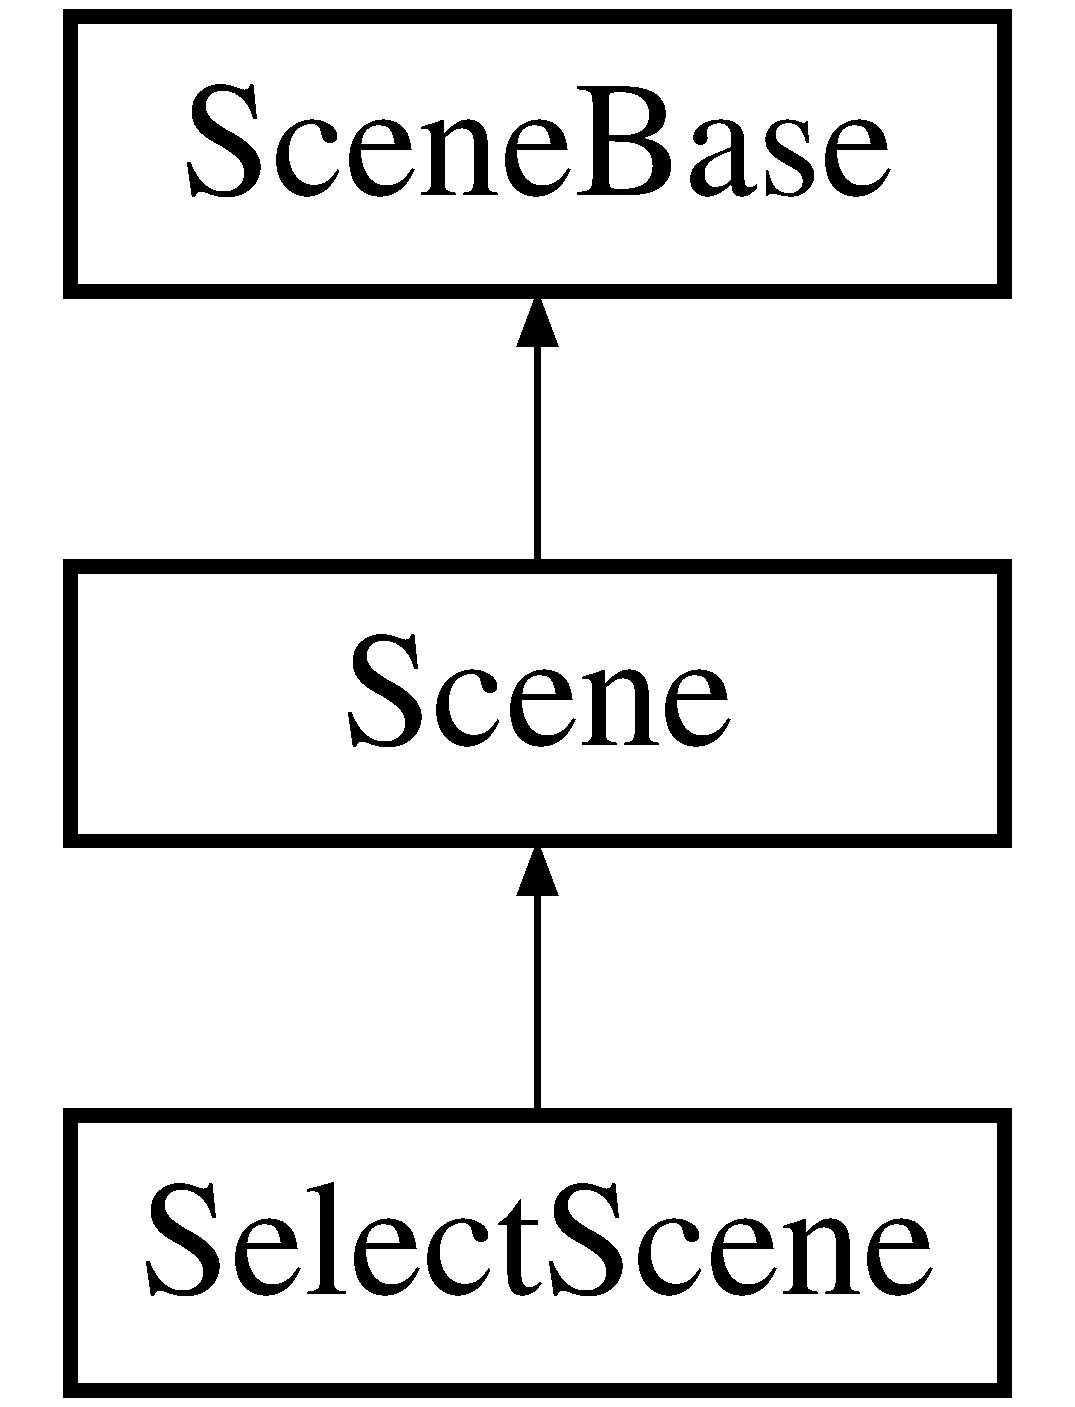
\includegraphics[height=3.000000cm]{class_select_scene}
\end{center}
\end{figure}
\subsection*{公開メンバ関数}
\begin{DoxyCompactItemize}
\item 
void \mbox{\hyperlink{class_select_scene_a20b3a902b5521d7494ed353731b3065d}{Init}} () final
\begin{DoxyCompactList}\small\item\em セレクトシーンの初期化 \end{DoxyCompactList}\item 
std\+::shared\+\_\+ptr$<$ \mbox{\hyperlink{class_scene}{Scene}} $>$ \mbox{\hyperlink{class_select_scene_a0cef696ddf74155e061cc5f9f2e06419}{Update}} (std\+::shared\+\_\+ptr$<$ \mbox{\hyperlink{class_scene}{Scene}} $>$ \&) final
\begin{DoxyCompactList}\small\item\em セレクトシーンの更新 \end{DoxyCompactList}\item 
void \mbox{\hyperlink{class_select_scene_a85445536ad84d5232c724ecb7d48b8aa}{Render}} () final
\begin{DoxyCompactList}\small\item\em セレクトシーンの描画 \end{DoxyCompactList}\item 
void \mbox{\hyperlink{class_select_scene_a938293516c0e1ae5bb09dbab81bc78d9}{Destroy}} () final
\begin{DoxyCompactList}\small\item\em セレクトシーンの破棄 \end{DoxyCompactList}\item 
void \mbox{\hyperlink{class_select_scene_a546190bc143f6d7a3055935f97b55596}{Exit\+Fade\+Update}} () final
\begin{DoxyCompactList}\small\item\em フェード中の更新 \end{DoxyCompactList}\end{DoxyCompactItemize}


\subsection{詳解}
セレクトシーンクラス 

\subsection{関数詳解}
\mbox{\Hypertarget{class_select_scene_a938293516c0e1ae5bb09dbab81bc78d9}\label{class_select_scene_a938293516c0e1ae5bb09dbab81bc78d9}} 
\index{Select\+Scene@{Select\+Scene}!Destroy@{Destroy}}
\index{Destroy@{Destroy}!Select\+Scene@{Select\+Scene}}
\subsubsection{\texorpdfstring{Destroy()}{Destroy()}}
{\footnotesize\ttfamily void Select\+Scene\+::\+Destroy (\begin{DoxyParamCaption}{ }\end{DoxyParamCaption})\hspace{0.3cm}{\ttfamily [final]}, {\ttfamily [virtual]}}



セレクトシーンの破棄 



\mbox{\hyperlink{class_scene_base_a7c5b54020bc519b4dadfe9770d6b27f7}{Scene\+Base}}を実装しています。

\mbox{\Hypertarget{class_select_scene_a546190bc143f6d7a3055935f97b55596}\label{class_select_scene_a546190bc143f6d7a3055935f97b55596}} 
\index{Select\+Scene@{Select\+Scene}!Exit\+Fade\+Update@{Exit\+Fade\+Update}}
\index{Exit\+Fade\+Update@{Exit\+Fade\+Update}!Select\+Scene@{Select\+Scene}}
\subsubsection{\texorpdfstring{Exit\+Fade\+Update()}{ExitFadeUpdate()}}
{\footnotesize\ttfamily void Select\+Scene\+::\+Exit\+Fade\+Update (\begin{DoxyParamCaption}{ }\end{DoxyParamCaption})\hspace{0.3cm}{\ttfamily [final]}, {\ttfamily [virtual]}}



フェード中の更新 



\mbox{\hyperlink{class_scene_ad19a449c6ed452823dae14183689570c}{Scene}}を再実装しています。

\mbox{\Hypertarget{class_select_scene_a20b3a902b5521d7494ed353731b3065d}\label{class_select_scene_a20b3a902b5521d7494ed353731b3065d}} 
\index{Select\+Scene@{Select\+Scene}!Init@{Init}}
\index{Init@{Init}!Select\+Scene@{Select\+Scene}}
\subsubsection{\texorpdfstring{Init()}{Init()}}
{\footnotesize\ttfamily void Select\+Scene\+::\+Init (\begin{DoxyParamCaption}{ }\end{DoxyParamCaption})\hspace{0.3cm}{\ttfamily [final]}, {\ttfamily [virtual]}}



セレクトシーンの初期化 



\mbox{\hyperlink{class_scene_base_a24d7db43c819924dc8b07b436f6d3148}{Scene\+Base}}を実装しています。

\mbox{\Hypertarget{class_select_scene_a85445536ad84d5232c724ecb7d48b8aa}\label{class_select_scene_a85445536ad84d5232c724ecb7d48b8aa}} 
\index{Select\+Scene@{Select\+Scene}!Render@{Render}}
\index{Render@{Render}!Select\+Scene@{Select\+Scene}}
\subsubsection{\texorpdfstring{Render()}{Render()}}
{\footnotesize\ttfamily void Select\+Scene\+::\+Render (\begin{DoxyParamCaption}{ }\end{DoxyParamCaption})\hspace{0.3cm}{\ttfamily [final]}, {\ttfamily [virtual]}}



セレクトシーンの描画 



\mbox{\hyperlink{class_scene_base_ad981674ce731ea267f398e889bbb9dc3}{Scene\+Base}}を実装しています。

\mbox{\Hypertarget{class_select_scene_a0cef696ddf74155e061cc5f9f2e06419}\label{class_select_scene_a0cef696ddf74155e061cc5f9f2e06419}} 
\index{Select\+Scene@{Select\+Scene}!Update@{Update}}
\index{Update@{Update}!Select\+Scene@{Select\+Scene}}
\subsubsection{\texorpdfstring{Update()}{Update()}}
{\footnotesize\ttfamily std\+::shared\+\_\+ptr$<$ \mbox{\hyperlink{class_scene}{Scene}} $>$ Select\+Scene\+::\+Update (\begin{DoxyParamCaption}\item[{std\+::shared\+\_\+ptr$<$ \mbox{\hyperlink{class_scene}{Scene}} $>$ \&}]{scene }\end{DoxyParamCaption})\hspace{0.3cm}{\ttfamily [final]}, {\ttfamily [virtual]}}



セレクトシーンの更新 

\begin{DoxyReturn}{戻り値}
std\+::shared\+\_\+ptr$<$\+Scene$>$ シーンが変わるなら次のシーンのstd\+::shared\+\_\+ptr$<$\+Scene$>$を返す 
\end{DoxyReturn}


\mbox{\hyperlink{class_scene_ab71ee5f19764b90c87b4574aa1cb1d25}{Scene}}を実装しています。



このクラス詳解は次のファイルから抽出されました\+:\begin{DoxyCompactItemize}
\item 
C\+:/\+Users/tokir/\+Documents/\+Git\+Hub/\+Weapon\+Merchant\+Adventure/src/src/scene/main/select/\mbox{\hyperlink{select__scene_8h}{select\+\_\+scene.\+h}}\item 
C\+:/\+Users/tokir/\+Documents/\+Git\+Hub/\+Weapon\+Merchant\+Adventure/src/src/scene/main/select/\mbox{\hyperlink{select__scene_8cpp}{select\+\_\+scene.\+cpp}}\end{DoxyCompactItemize}

\hypertarget{class_singleton}{}\section{Singleton$<$ T $>$ クラステンプレート}
\label{class_singleton}\index{Singleton$<$ T $>$@{Singleton$<$ T $>$}}


Singletonテンプレートスーパークラス  




{\ttfamily \#include $<$singleton.\+h$>$}

\subsection*{公開メンバ関数}
\begin{DoxyCompactItemize}
\item 
virtual \mbox{\hyperlink{class_singleton_ad3c93143836479fb3dd96b21b795938c}{$\sim$\+Singleton}} ()
\end{DoxyCompactItemize}
\subsection*{静的公開メンバ関数}
\begin{DoxyCompactItemize}
\item 
static std\+::unique\+\_\+ptr$<$ T $>$ \& \mbox{\hyperlink{class_singleton_a57b10e4aa6d89bbac3a16355914655b3}{Get\+Instance}} ()
\begin{DoxyCompactList}\small\item\em インスタンスの取得 \end{DoxyCompactList}\end{DoxyCompactItemize}
\subsection*{限定公開メンバ関数}
\begin{DoxyCompactItemize}
\item 
\mbox{\hyperlink{class_singleton_a923b995920da9c06590adb170ab2f890}{Singleton}} ()
\end{DoxyCompactItemize}


\subsection{詳解}
\subsubsection*{template$<$typename T$>$\newline
class Singleton$<$ T $>$}

Singletonテンプレートスーパークラス 

publicで仮引数にそのクラスを入れて継承するとそのクラスが\+Singletonになる 

\subsection{構築子と解体子}
\mbox{\Hypertarget{class_singleton_ad3c93143836479fb3dd96b21b795938c}\label{class_singleton_ad3c93143836479fb3dd96b21b795938c}} 
\index{Singleton@{Singleton}!````~Singleton@{$\sim$\+Singleton}}
\index{````~Singleton@{$\sim$\+Singleton}!Singleton@{Singleton}}
\subsubsection{\texorpdfstring{$\sim$\+Singleton()}{~Singleton()}}
{\footnotesize\ttfamily template$<$typename T$>$ \\
virtual \mbox{\hyperlink{class_singleton}{Singleton}}$<$ T $>$\+::$\sim$\mbox{\hyperlink{class_singleton}{Singleton}} (\begin{DoxyParamCaption}{ }\end{DoxyParamCaption})\hspace{0.3cm}{\ttfamily [inline]}, {\ttfamily [virtual]}}

\mbox{\Hypertarget{class_singleton_a923b995920da9c06590adb170ab2f890}\label{class_singleton_a923b995920da9c06590adb170ab2f890}} 
\index{Singleton@{Singleton}!Singleton@{Singleton}}
\index{Singleton@{Singleton}!Singleton@{Singleton}}
\subsubsection{\texorpdfstring{Singleton()}{Singleton()}}
{\footnotesize\ttfamily template$<$typename T$>$ \\
\mbox{\hyperlink{class_singleton}{Singleton}}$<$ T $>$\+::\mbox{\hyperlink{class_singleton}{Singleton}} (\begin{DoxyParamCaption}{ }\end{DoxyParamCaption})\hspace{0.3cm}{\ttfamily [inline]}, {\ttfamily [protected]}}



\subsection{関数詳解}
\mbox{\Hypertarget{class_singleton_a57b10e4aa6d89bbac3a16355914655b3}\label{class_singleton_a57b10e4aa6d89bbac3a16355914655b3}} 
\index{Singleton@{Singleton}!Get\+Instance@{Get\+Instance}}
\index{Get\+Instance@{Get\+Instance}!Singleton@{Singleton}}
\subsubsection{\texorpdfstring{Get\+Instance()}{GetInstance()}}
{\footnotesize\ttfamily template$<$typename T$>$ \\
static std\+::unique\+\_\+ptr$<$T$>$\& \mbox{\hyperlink{class_singleton}{Singleton}}$<$ T $>$\+::Get\+Instance (\begin{DoxyParamCaption}{ }\end{DoxyParamCaption})\hspace{0.3cm}{\ttfamily [inline]}, {\ttfamily [static]}}



インスタンスの取得 

\begin{DoxyReturn}{戻り値}
std\+::unique\+\_\+ptr$<$\+T$>$\& インスタンス 
\end{DoxyReturn}


このクラス詳解は次のファイルから抽出されました\+:\begin{DoxyCompactItemize}
\item 
C\+:/\+Users/tokir/\+Documents/\+Git\+Hub/\+Weapon\+Merchant\+Adventure/src/common/\mbox{\hyperlink{singleton_8h}{singleton.\+h}}\end{DoxyCompactItemize}

\hypertarget{class_sound}{}\section{Sound クラス}
\label{class_sound}\index{Sound@{Sound}}


 個々のサウンドクラス  




{\ttfamily \#include $<$sound.\+h$>$}

\subsection*{公開メンバ関数}
\begin{DoxyCompactItemize}
\item 
void \mbox{\hyperlink{class_sound_a3c8007c8e52bf541fc81adfa4b340b0f}{Init}} (W\+C\+H\+AR $\ast$, bool, bool)
\begin{DoxyCompactList}\small\item\em サウンドの初期化 \end{DoxyCompactList}\item 
void \mbox{\hyperlink{class_sound_ae021b518e93d7d8c6f3ea951cd4b98d8}{Start}} ()
\item 
void \mbox{\hyperlink{class_sound_a188de6836d531813da378464e392e813}{Stop}} ()
\item 
void \mbox{\hyperlink{class_sound_a4e199b4346519a4977fe94998c4a77e7}{Pause}} ()
\item 
void \mbox{\hyperlink{class_sound_a993eee69f61611ca1b4621ea0952e2c8}{Set\+Volume}} (float vol)
\item 
void \mbox{\hyperlink{class_sound_a06b9680efb2b6b41b52d9f25ac0264f1}{Set\+Pitch}} (float pit)
\item 
void \mbox{\hyperlink{class_sound_a1b066e78405656b1475849139ca24dce}{Set\+Pan}} (float pan)
\item 
\mbox{\hyperlink{class_sound_a0907389078bf740be2a5763366ad3376}{$\sim$\+Sound}} ()
\begin{DoxyCompactList}\small\item\em デストラクタ \end{DoxyCompactList}\item 
std\+::unique\+\_\+ptr$<$ Direct\+X\+::\+Sound\+Effect\+Instance $>$ \& \mbox{\hyperlink{class_sound_a0d79b20f421c0020c53b08c05b6df25b}{operator()}} ()
\end{DoxyCompactItemize}


\subsection{詳解}
 個々のサウンドクラス 

\subsection{構築子と解体子}
\mbox{\Hypertarget{class_sound_a0907389078bf740be2a5763366ad3376}\label{class_sound_a0907389078bf740be2a5763366ad3376}} 
\index{Sound@{Sound}!````~Sound@{$\sim$\+Sound}}
\index{````~Sound@{$\sim$\+Sound}!Sound@{Sound}}
\subsubsection{\texorpdfstring{$\sim$\+Sound()}{~Sound()}}
{\footnotesize\ttfamily Sound\+::$\sim$\+Sound (\begin{DoxyParamCaption}{ }\end{DoxyParamCaption})}



デストラクタ 



\subsection{関数詳解}
\mbox{\Hypertarget{class_sound_a3c8007c8e52bf541fc81adfa4b340b0f}\label{class_sound_a3c8007c8e52bf541fc81adfa4b340b0f}} 
\index{Sound@{Sound}!Init@{Init}}
\index{Init@{Init}!Sound@{Sound}}
\subsubsection{\texorpdfstring{Init()}{Init()}}
{\footnotesize\ttfamily void Sound\+::\+Init (\begin{DoxyParamCaption}\item[{W\+C\+H\+AR $\ast$}]{path,  }\item[{bool}]{loop,  }\item[{bool}]{awake }\end{DoxyParamCaption})}



サウンドの初期化 


\begin{DoxyParams}{引数}
{\em path} & サウンドのパス \\
\hline
{\em loop} & ループするかどうか \\
\hline
{\em awake} & 初期化した瞬間から再生するかどうか \\
\hline
\end{DoxyParams}
\mbox{\Hypertarget{class_sound_a0d79b20f421c0020c53b08c05b6df25b}\label{class_sound_a0d79b20f421c0020c53b08c05b6df25b}} 
\index{Sound@{Sound}!operator()@{operator()}}
\index{operator()@{operator()}!Sound@{Sound}}
\subsubsection{\texorpdfstring{operator()()}{operator()()}}
{\footnotesize\ttfamily std\+::unique\+\_\+ptr$<$Direct\+X\+::\+Sound\+Effect\+Instance$>$\& Sound\+::operator() (\begin{DoxyParamCaption}{ }\end{DoxyParamCaption})\hspace{0.3cm}{\ttfamily [inline]}}

\mbox{\Hypertarget{class_sound_a4e199b4346519a4977fe94998c4a77e7}\label{class_sound_a4e199b4346519a4977fe94998c4a77e7}} 
\index{Sound@{Sound}!Pause@{Pause}}
\index{Pause@{Pause}!Sound@{Sound}}
\subsubsection{\texorpdfstring{Pause()}{Pause()}}
{\footnotesize\ttfamily void Sound\+::\+Pause (\begin{DoxyParamCaption}{ }\end{DoxyParamCaption})\hspace{0.3cm}{\ttfamily [inline]}}

\mbox{\Hypertarget{class_sound_a1b066e78405656b1475849139ca24dce}\label{class_sound_a1b066e78405656b1475849139ca24dce}} 
\index{Sound@{Sound}!Set\+Pan@{Set\+Pan}}
\index{Set\+Pan@{Set\+Pan}!Sound@{Sound}}
\subsubsection{\texorpdfstring{Set\+Pan()}{SetPan()}}
{\footnotesize\ttfamily void Sound\+::\+Set\+Pan (\begin{DoxyParamCaption}\item[{float}]{pan }\end{DoxyParamCaption})\hspace{0.3cm}{\ttfamily [inline]}}

\mbox{\Hypertarget{class_sound_a06b9680efb2b6b41b52d9f25ac0264f1}\label{class_sound_a06b9680efb2b6b41b52d9f25ac0264f1}} 
\index{Sound@{Sound}!Set\+Pitch@{Set\+Pitch}}
\index{Set\+Pitch@{Set\+Pitch}!Sound@{Sound}}
\subsubsection{\texorpdfstring{Set\+Pitch()}{SetPitch()}}
{\footnotesize\ttfamily void Sound\+::\+Set\+Pitch (\begin{DoxyParamCaption}\item[{float}]{pit }\end{DoxyParamCaption})\hspace{0.3cm}{\ttfamily [inline]}}

\mbox{\Hypertarget{class_sound_a993eee69f61611ca1b4621ea0952e2c8}\label{class_sound_a993eee69f61611ca1b4621ea0952e2c8}} 
\index{Sound@{Sound}!Set\+Volume@{Set\+Volume}}
\index{Set\+Volume@{Set\+Volume}!Sound@{Sound}}
\subsubsection{\texorpdfstring{Set\+Volume()}{SetVolume()}}
{\footnotesize\ttfamily void Sound\+::\+Set\+Volume (\begin{DoxyParamCaption}\item[{float}]{vol }\end{DoxyParamCaption})\hspace{0.3cm}{\ttfamily [inline]}}

\mbox{\Hypertarget{class_sound_ae021b518e93d7d8c6f3ea951cd4b98d8}\label{class_sound_ae021b518e93d7d8c6f3ea951cd4b98d8}} 
\index{Sound@{Sound}!Start@{Start}}
\index{Start@{Start}!Sound@{Sound}}
\subsubsection{\texorpdfstring{Start()}{Start()}}
{\footnotesize\ttfamily void Sound\+::\+Start (\begin{DoxyParamCaption}{ }\end{DoxyParamCaption})\hspace{0.3cm}{\ttfamily [inline]}}

\mbox{\Hypertarget{class_sound_a188de6836d531813da378464e392e813}\label{class_sound_a188de6836d531813da378464e392e813}} 
\index{Sound@{Sound}!Stop@{Stop}}
\index{Stop@{Stop}!Sound@{Sound}}
\subsubsection{\texorpdfstring{Stop()}{Stop()}}
{\footnotesize\ttfamily void Sound\+::\+Stop (\begin{DoxyParamCaption}{ }\end{DoxyParamCaption})\hspace{0.3cm}{\ttfamily [inline]}}



このクラス詳解は次のファイルから抽出されました\+:\begin{DoxyCompactItemize}
\item 
C\+:/\+Users/tokir/\+Documents/\+Git\+Hub/\+Weapon\+Merchant\+Adventure/src/sound/\mbox{\hyperlink{sound_8h}{sound.\+h}}\item 
C\+:/\+Users/tokir/\+Documents/\+Git\+Hub/\+Weapon\+Merchant\+Adventure/src/sound/\mbox{\hyperlink{sound_8cpp}{sound.\+cpp}}\end{DoxyCompactItemize}

\hypertarget{class_sound_manager}{}\section{Sound\+Manager クラス}
\label{class_sound_manager}\index{Sound\+Manager@{Sound\+Manager}}


サウンドを管理するクラス  




{\ttfamily \#include $<$sound\+\_\+manager.\+h$>$}

Sound\+Manager の継承関係図\begin{figure}[H]
\begin{center}
\leavevmode
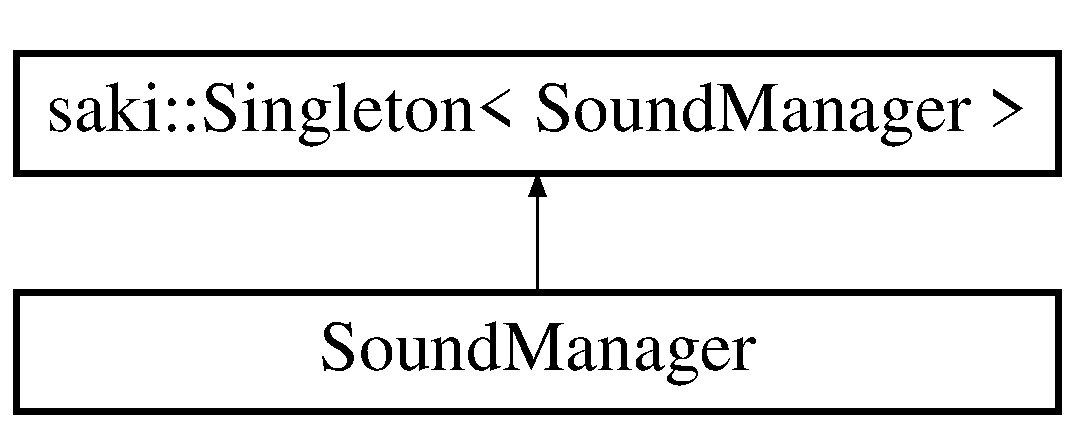
\includegraphics[height=2.000000cm]{class_sound_manager}
\end{center}
\end{figure}
\subsection*{公開メンバ関数}
\begin{DoxyCompactItemize}
\item 
std\+::unique\+\_\+ptr$<$ Direct\+X\+::\+Sound\+Effect $>$ \& \mbox{\hyperlink{class_sound_manager_a3ba4b2fe49cdc051f33aa800851f8b98}{Get\+Sound}} (W\+C\+H\+AR $\ast$)
\begin{DoxyCompactList}\small\item\em サウンドを返す \end{DoxyCompactList}\item 
void \mbox{\hyperlink{class_sound_manager_adab2bc016911756ffd973c7d781b5cfb}{Init}} (H\+W\+ND)
\begin{DoxyCompactList}\small\item\em サウンドマネージャークラスの初期化 \end{DoxyCompactList}\item 
void \mbox{\hyperlink{class_sound_manager_aaf241621221cdbefeba78e8b6bc29240}{Update}} ()
\begin{DoxyCompactList}\small\item\em サウンドマネージャーの更新 \end{DoxyCompactList}\item 
void \mbox{\hyperlink{class_sound_manager_abf0d473d0a31323c8e74684976b08e7f}{Destroy}} ()
\begin{DoxyCompactList}\small\item\em サウンドマネージャーの破棄 \end{DoxyCompactList}\item 
auto \mbox{\hyperlink{class_sound_manager_a5a575ac572eb0b50b3bb48b879a1a7e6}{Get\+Engine}} () const
\item 
void \mbox{\hyperlink{class_sound_manager_acc9fb61509f30c7eb9136386eeeb9f94}{Retry\+Audio}} ()
\item 
void \mbox{\hyperlink{class_sound_manager_a97d76cb22596fbb3c85766df0dcde757}{Suspend}} ()
\item 
void \mbox{\hyperlink{class_sound_manager_a6107940d2299131fbd7991a4f222491b}{Resume}} ()
\end{DoxyCompactItemize}
\subsection*{その他の継承メンバ}


\subsection{詳解}
サウンドを管理するクラス 

\subsection{関数詳解}
\mbox{\Hypertarget{class_sound_manager_abf0d473d0a31323c8e74684976b08e7f}\label{class_sound_manager_abf0d473d0a31323c8e74684976b08e7f}} 
\index{Sound\+Manager@{Sound\+Manager}!Destroy@{Destroy}}
\index{Destroy@{Destroy}!Sound\+Manager@{Sound\+Manager}}
\subsubsection{\texorpdfstring{Destroy()}{Destroy()}}
{\footnotesize\ttfamily void Sound\+Manager\+::\+Destroy (\begin{DoxyParamCaption}{ }\end{DoxyParamCaption})}



サウンドマネージャーの破棄 

\mbox{\Hypertarget{class_sound_manager_a5a575ac572eb0b50b3bb48b879a1a7e6}\label{class_sound_manager_a5a575ac572eb0b50b3bb48b879a1a7e6}} 
\index{Sound\+Manager@{Sound\+Manager}!Get\+Engine@{Get\+Engine}}
\index{Get\+Engine@{Get\+Engine}!Sound\+Manager@{Sound\+Manager}}
\subsubsection{\texorpdfstring{Get\+Engine()}{GetEngine()}}
{\footnotesize\ttfamily auto Sound\+Manager\+::\+Get\+Engine (\begin{DoxyParamCaption}{ }\end{DoxyParamCaption}) const\hspace{0.3cm}{\ttfamily [inline]}}

\mbox{\Hypertarget{class_sound_manager_a3ba4b2fe49cdc051f33aa800851f8b98}\label{class_sound_manager_a3ba4b2fe49cdc051f33aa800851f8b98}} 
\index{Sound\+Manager@{Sound\+Manager}!Get\+Sound@{Get\+Sound}}
\index{Get\+Sound@{Get\+Sound}!Sound\+Manager@{Sound\+Manager}}
\subsubsection{\texorpdfstring{Get\+Sound()}{GetSound()}}
{\footnotesize\ttfamily std\+::unique\+\_\+ptr$<$ Direct\+X\+::\+Sound\+Effect $>$ \& Sound\+Manager\+::\+Get\+Sound (\begin{DoxyParamCaption}\item[{W\+C\+H\+AR $\ast$}]{path }\end{DoxyParamCaption})}



サウンドを返す 


\begin{DoxyParams}{引数}
{\em path} & wavファイルのパス\\
\hline
\end{DoxyParams}
同じファイルを2度読み込まないようにする \mbox{\Hypertarget{class_sound_manager_adab2bc016911756ffd973c7d781b5cfb}\label{class_sound_manager_adab2bc016911756ffd973c7d781b5cfb}} 
\index{Sound\+Manager@{Sound\+Manager}!Init@{Init}}
\index{Init@{Init}!Sound\+Manager@{Sound\+Manager}}
\subsubsection{\texorpdfstring{Init()}{Init()}}
{\footnotesize\ttfamily void Sound\+Manager\+::\+Init (\begin{DoxyParamCaption}\item[{H\+W\+ND}]{h\+Wnd }\end{DoxyParamCaption})}



サウンドマネージャークラスの初期化 


\begin{DoxyParams}{引数}
{\em h\+Wnd} & ウィンドウハンドラ \\
\hline
\end{DoxyParams}
\mbox{\Hypertarget{class_sound_manager_a6107940d2299131fbd7991a4f222491b}\label{class_sound_manager_a6107940d2299131fbd7991a4f222491b}} 
\index{Sound\+Manager@{Sound\+Manager}!Resume@{Resume}}
\index{Resume@{Resume}!Sound\+Manager@{Sound\+Manager}}
\subsubsection{\texorpdfstring{Resume()}{Resume()}}
{\footnotesize\ttfamily void Sound\+Manager\+::\+Resume (\begin{DoxyParamCaption}{ }\end{DoxyParamCaption})\hspace{0.3cm}{\ttfamily [inline]}}

\mbox{\Hypertarget{class_sound_manager_acc9fb61509f30c7eb9136386eeeb9f94}\label{class_sound_manager_acc9fb61509f30c7eb9136386eeeb9f94}} 
\index{Sound\+Manager@{Sound\+Manager}!Retry\+Audio@{Retry\+Audio}}
\index{Retry\+Audio@{Retry\+Audio}!Sound\+Manager@{Sound\+Manager}}
\subsubsection{\texorpdfstring{Retry\+Audio()}{RetryAudio()}}
{\footnotesize\ttfamily void Sound\+Manager\+::\+Retry\+Audio (\begin{DoxyParamCaption}{ }\end{DoxyParamCaption})\hspace{0.3cm}{\ttfamily [inline]}}

\mbox{\Hypertarget{class_sound_manager_a97d76cb22596fbb3c85766df0dcde757}\label{class_sound_manager_a97d76cb22596fbb3c85766df0dcde757}} 
\index{Sound\+Manager@{Sound\+Manager}!Suspend@{Suspend}}
\index{Suspend@{Suspend}!Sound\+Manager@{Sound\+Manager}}
\subsubsection{\texorpdfstring{Suspend()}{Suspend()}}
{\footnotesize\ttfamily void Sound\+Manager\+::\+Suspend (\begin{DoxyParamCaption}{ }\end{DoxyParamCaption})\hspace{0.3cm}{\ttfamily [inline]}}

\mbox{\Hypertarget{class_sound_manager_aaf241621221cdbefeba78e8b6bc29240}\label{class_sound_manager_aaf241621221cdbefeba78e8b6bc29240}} 
\index{Sound\+Manager@{Sound\+Manager}!Update@{Update}}
\index{Update@{Update}!Sound\+Manager@{Sound\+Manager}}
\subsubsection{\texorpdfstring{Update()}{Update()}}
{\footnotesize\ttfamily void Sound\+Manager\+::\+Update (\begin{DoxyParamCaption}{ }\end{DoxyParamCaption})}



サウンドマネージャーの更新 



このクラス詳解は次のファイルから抽出されました\+:\begin{DoxyCompactItemize}
\item 
C\+:/\+Users/tokir/\+Documents/\+Git\+Hub/\+Weapon\+Merchant\+Adventure/src/sound/manager/\mbox{\hyperlink{sound__manager_8h}{sound\+\_\+manager.\+h}}\item 
C\+:/\+Users/tokir/\+Documents/\+Git\+Hub/\+Weapon\+Merchant\+Adventure/src/sound/manager/\mbox{\hyperlink{sound__manager_8cpp}{sound\+\_\+manager.\+cpp}}\end{DoxyCompactItemize}

\hypertarget{class_sprite}{}\section{Sprite クラス}
\label{class_sprite}\index{Sprite@{Sprite}}


{\ttfamily \#include $<$sprite.\+h$>$}

\subsection*{公開メンバ関数}
\begin{DoxyCompactItemize}
\item 
H\+R\+E\+S\+U\+LT \mbox{\hyperlink{class_sprite_a65b9b470731149992bfa7401ffb676ae}{Init}} (const std\+::string \&, const W\+C\+H\+AR $\ast$, \mbox{\hyperlink{common_8h_ae148fff5818e9444b4ab2288829559bf}{Vec2}} \&, const std\+::string \&=\char`\"{}shader\char`\"{}, const W\+C\+H\+AR $\ast$=L\char`\"{}sprite\+\_\+shader.\+hlsl\char`\"{}, const W\+C\+H\+AR $\ast$=L\char`\"{}sprite\+\_\+shader.\+hlsl\char`\"{}, const float=1, const float=1, const float=1, const float=1)
\item 
void \mbox{\hyperlink{class_sprite_a23296a54e3165adbbeb2b5351d04b921}{Render}} (const \mbox{\hyperlink{common_8h_a1c43cb8f0d8a41901f3ce4c67dbbce20}{Transform}} \&, const bool=true)
\item 
void \mbox{\hyperlink{class_sprite_a0a3daa8677d1205981e27bd698025afa}{Color\+Change}} (const float r, const float g, const float b, const float a)
\end{DoxyCompactItemize}
\subsection*{公開変数類}
\begin{DoxyCompactItemize}
\item 
\mbox{\hyperlink{common_8h_ae148fff5818e9444b4ab2288829559bf}{Vec2}} \mbox{\hyperlink{class_sprite_aac62c18a9b678d357f3465d45b2e6ebd}{slice\+\_\+num}}
\item 
\mbox{\hyperlink{common_8h_ae148fff5818e9444b4ab2288829559bf}{Vec2}} \mbox{\hyperlink{class_sprite_a5c96c0e7d46a79740a5fe9e71e9f132b}{prev\+\_\+slice}}
\item 
\mbox{\hyperlink{common_8h_ae148fff5818e9444b4ab2288829559bf}{Vec2}} \mbox{\hyperlink{class_sprite_a7d4903c9693bbb41094b395fe587bf47}{current\+\_\+slice}}
\item 
\mbox{\hyperlink{common_8h_ae148fff5818e9444b4ab2288829559bf}{Vec2}} \mbox{\hyperlink{class_sprite_afb8f3dc3f60aaa09306153d50e4243c9}{texture\+\_\+size}}
\item 
bool \mbox{\hyperlink{class_sprite_ae561a927089192371cff0c1b7402593b}{is\+\_\+ui\+\_\+image}} = false
\item 
float \mbox{\hyperlink{class_sprite_a4e306b23bbc378d1d973ca61084ebd9e}{percent}} = 1.\+0f
\end{DoxyCompactItemize}
\subsection*{静的公開変数類}
\begin{DoxyCompactItemize}
\item 
static int \mbox{\hyperlink{class_sprite_a9acc35b192b4150fe31b9386f7f9fc78}{depth}} = 9999
\item 
static bool \mbox{\hyperlink{class_sprite_ad4340ffd8b88519c28822eb2e9b71bf0}{has\+\_\+target}} = false
\item 
static float \mbox{\hyperlink{class_sprite_add18808500d3dca23d496757bf10259a}{target\+\_\+x}} = 0
\end{DoxyCompactItemize}


\subsection{関数詳解}
\mbox{\Hypertarget{class_sprite_a0a3daa8677d1205981e27bd698025afa}\label{class_sprite_a0a3daa8677d1205981e27bd698025afa}} 
\index{Sprite@{Sprite}!Color\+Change@{Color\+Change}}
\index{Color\+Change@{Color\+Change}!Sprite@{Sprite}}
\subsubsection{\texorpdfstring{Color\+Change()}{ColorChange()}}
{\footnotesize\ttfamily void Sprite\+::\+Color\+Change (\begin{DoxyParamCaption}\item[{const float}]{r,  }\item[{const float}]{g,  }\item[{const float}]{b,  }\item[{const float}]{a }\end{DoxyParamCaption})\hspace{0.3cm}{\ttfamily [inline]}}

\mbox{\Hypertarget{class_sprite_a65b9b470731149992bfa7401ffb676ae}\label{class_sprite_a65b9b470731149992bfa7401ffb676ae}} 
\index{Sprite@{Sprite}!Init@{Init}}
\index{Init@{Init}!Sprite@{Sprite}}
\subsubsection{\texorpdfstring{Init()}{Init()}}
{\footnotesize\ttfamily H\+R\+E\+S\+U\+LT Sprite\+::\+Init (\begin{DoxyParamCaption}\item[{const std\+::string \&}]{texture\+\_\+name,  }\item[{const W\+C\+H\+AR $\ast$}]{texture\+\_\+path,  }\item[{\mbox{\hyperlink{common_8h_ae148fff5818e9444b4ab2288829559bf}{Vec2}} \&}]{size,  }\item[{const std\+::string \&}]{shader\+\_\+name = {\ttfamily \char`\"{}shader\char`\"{}},  }\item[{const W\+C\+H\+AR $\ast$}]{v\+\_\+shader\+\_\+path = {\ttfamily L\char`\"{}sprite\+\_\+shader.hlsl\char`\"{}},  }\item[{const W\+C\+H\+AR $\ast$}]{p\+\_\+shader\+\_\+path = {\ttfamily L\char`\"{}sprite\+\_\+shader.hlsl\char`\"{}},  }\item[{const float}]{slice\+\_\+h\+\_\+num = {\ttfamily 1},  }\item[{const float}]{slice\+\_\+v\+\_\+num = {\ttfamily 1},  }\item[{const float}]{slice\+\_\+h\+\_\+init = {\ttfamily 1},  }\item[{const float}]{slice\+\_\+v\+\_\+init = {\ttfamily 1} }\end{DoxyParamCaption})}

\mbox{\Hypertarget{class_sprite_a23296a54e3165adbbeb2b5351d04b921}\label{class_sprite_a23296a54e3165adbbeb2b5351d04b921}} 
\index{Sprite@{Sprite}!Render@{Render}}
\index{Render@{Render}!Sprite@{Sprite}}
\subsubsection{\texorpdfstring{Render()}{Render()}}
{\footnotesize\ttfamily void Sprite\+::\+Render (\begin{DoxyParamCaption}\item[{const \mbox{\hyperlink{common_8h_a1c43cb8f0d8a41901f3ce4c67dbbce20}{Transform}} \&}]{transform,  }\item[{const bool}]{camera\+\_\+affected = {\ttfamily true} }\end{DoxyParamCaption})}



\subsection{メンバ詳解}
\mbox{\Hypertarget{class_sprite_a7d4903c9693bbb41094b395fe587bf47}\label{class_sprite_a7d4903c9693bbb41094b395fe587bf47}} 
\index{Sprite@{Sprite}!current\+\_\+slice@{current\+\_\+slice}}
\index{current\+\_\+slice@{current\+\_\+slice}!Sprite@{Sprite}}
\subsubsection{\texorpdfstring{current\+\_\+slice}{current\_slice}}
{\footnotesize\ttfamily \mbox{\hyperlink{common_8h_ae148fff5818e9444b4ab2288829559bf}{Vec2}} Sprite\+::current\+\_\+slice}

\mbox{\Hypertarget{class_sprite_a9acc35b192b4150fe31b9386f7f9fc78}\label{class_sprite_a9acc35b192b4150fe31b9386f7f9fc78}} 
\index{Sprite@{Sprite}!depth@{depth}}
\index{depth@{depth}!Sprite@{Sprite}}
\subsubsection{\texorpdfstring{depth}{depth}}
{\footnotesize\ttfamily int Sprite\+::depth = 9999\hspace{0.3cm}{\ttfamily [static]}}

\mbox{\Hypertarget{class_sprite_ad4340ffd8b88519c28822eb2e9b71bf0}\label{class_sprite_ad4340ffd8b88519c28822eb2e9b71bf0}} 
\index{Sprite@{Sprite}!has\+\_\+target@{has\+\_\+target}}
\index{has\+\_\+target@{has\+\_\+target}!Sprite@{Sprite}}
\subsubsection{\texorpdfstring{has\+\_\+target}{has\_target}}
{\footnotesize\ttfamily bool Sprite\+::has\+\_\+target = false\hspace{0.3cm}{\ttfamily [static]}}

\mbox{\Hypertarget{class_sprite_ae561a927089192371cff0c1b7402593b}\label{class_sprite_ae561a927089192371cff0c1b7402593b}} 
\index{Sprite@{Sprite}!is\+\_\+ui\+\_\+image@{is\+\_\+ui\+\_\+image}}
\index{is\+\_\+ui\+\_\+image@{is\+\_\+ui\+\_\+image}!Sprite@{Sprite}}
\subsubsection{\texorpdfstring{is\+\_\+ui\+\_\+image}{is\_ui\_image}}
{\footnotesize\ttfamily bool Sprite\+::is\+\_\+ui\+\_\+image = false}

\mbox{\Hypertarget{class_sprite_a4e306b23bbc378d1d973ca61084ebd9e}\label{class_sprite_a4e306b23bbc378d1d973ca61084ebd9e}} 
\index{Sprite@{Sprite}!percent@{percent}}
\index{percent@{percent}!Sprite@{Sprite}}
\subsubsection{\texorpdfstring{percent}{percent}}
{\footnotesize\ttfamily float Sprite\+::percent = 1.\+0f}

\mbox{\Hypertarget{class_sprite_a5c96c0e7d46a79740a5fe9e71e9f132b}\label{class_sprite_a5c96c0e7d46a79740a5fe9e71e9f132b}} 
\index{Sprite@{Sprite}!prev\+\_\+slice@{prev\+\_\+slice}}
\index{prev\+\_\+slice@{prev\+\_\+slice}!Sprite@{Sprite}}
\subsubsection{\texorpdfstring{prev\+\_\+slice}{prev\_slice}}
{\footnotesize\ttfamily \mbox{\hyperlink{common_8h_ae148fff5818e9444b4ab2288829559bf}{Vec2}} Sprite\+::prev\+\_\+slice}

\mbox{\Hypertarget{class_sprite_aac62c18a9b678d357f3465d45b2e6ebd}\label{class_sprite_aac62c18a9b678d357f3465d45b2e6ebd}} 
\index{Sprite@{Sprite}!slice\+\_\+num@{slice\+\_\+num}}
\index{slice\+\_\+num@{slice\+\_\+num}!Sprite@{Sprite}}
\subsubsection{\texorpdfstring{slice\+\_\+num}{slice\_num}}
{\footnotesize\ttfamily \mbox{\hyperlink{common_8h_ae148fff5818e9444b4ab2288829559bf}{Vec2}} Sprite\+::slice\+\_\+num}

\mbox{\Hypertarget{class_sprite_add18808500d3dca23d496757bf10259a}\label{class_sprite_add18808500d3dca23d496757bf10259a}} 
\index{Sprite@{Sprite}!target\+\_\+x@{target\+\_\+x}}
\index{target\+\_\+x@{target\+\_\+x}!Sprite@{Sprite}}
\subsubsection{\texorpdfstring{target\+\_\+x}{target\_x}}
{\footnotesize\ttfamily float Sprite\+::target\+\_\+x = 0\hspace{0.3cm}{\ttfamily [static]}}

\mbox{\Hypertarget{class_sprite_afb8f3dc3f60aaa09306153d50e4243c9}\label{class_sprite_afb8f3dc3f60aaa09306153d50e4243c9}} 
\index{Sprite@{Sprite}!texture\+\_\+size@{texture\+\_\+size}}
\index{texture\+\_\+size@{texture\+\_\+size}!Sprite@{Sprite}}
\subsubsection{\texorpdfstring{texture\+\_\+size}{texture\_size}}
{\footnotesize\ttfamily \mbox{\hyperlink{common_8h_ae148fff5818e9444b4ab2288829559bf}{Vec2}} Sprite\+::texture\+\_\+size}



このクラス詳解は次のファイルから抽出されました\+:\begin{DoxyCompactItemize}
\item 
C\+:/\+Users/tokir/\+Documents/\+Git\+Hub/\+Weapon\+Merchant\+Adventure/src/src/sprite/\mbox{\hyperlink{sprite_8h}{sprite.\+h}}\item 
C\+:/\+Users/tokir/\+Documents/\+Git\+Hub/\+Weapon\+Merchant\+Adventure/src/src/sprite/\mbox{\hyperlink{sprite_8cpp}{sprite.\+cpp}}\end{DoxyCompactItemize}

\hypertarget{struct_sprite_color}{}\section{Sprite\+Color 構造体}
\label{struct_sprite_color}\index{Sprite\+Color@{Sprite\+Color}}


画像の色の構造体  




{\ttfamily \#include $<$sprite.\+h$>$}

\subsection*{公開変数類}
\begin{DoxyCompactItemize}
\item 
float \mbox{\hyperlink{struct_sprite_color_a640d8864838a78db2a9d5f1840e24882}{r}}
\item 
float \mbox{\hyperlink{struct_sprite_color_ae59c4c99310c60ac72740f83a3073a44}{g}}
\item 
float \mbox{\hyperlink{struct_sprite_color_ae99d1e9c97a11bd8c3db47a0ee9d45c1}{b}}
\item 
float \mbox{\hyperlink{struct_sprite_color_a82a19f7f0f96f706b9c4715eb87e0de8}{a}}
\end{DoxyCompactItemize}


\subsection{詳解}
画像の色の構造体 

\subsection{メンバ詳解}
\mbox{\Hypertarget{struct_sprite_color_a82a19f7f0f96f706b9c4715eb87e0de8}\label{struct_sprite_color_a82a19f7f0f96f706b9c4715eb87e0de8}} 
\index{Sprite\+Color@{Sprite\+Color}!a@{a}}
\index{a@{a}!Sprite\+Color@{Sprite\+Color}}
\subsubsection{\texorpdfstring{a}{a}}
{\footnotesize\ttfamily float Sprite\+Color\+::a}

\mbox{\Hypertarget{struct_sprite_color_ae99d1e9c97a11bd8c3db47a0ee9d45c1}\label{struct_sprite_color_ae99d1e9c97a11bd8c3db47a0ee9d45c1}} 
\index{Sprite\+Color@{Sprite\+Color}!b@{b}}
\index{b@{b}!Sprite\+Color@{Sprite\+Color}}
\subsubsection{\texorpdfstring{b}{b}}
{\footnotesize\ttfamily float Sprite\+Color\+::b}

\mbox{\Hypertarget{struct_sprite_color_ae59c4c99310c60ac72740f83a3073a44}\label{struct_sprite_color_ae59c4c99310c60ac72740f83a3073a44}} 
\index{Sprite\+Color@{Sprite\+Color}!g@{g}}
\index{g@{g}!Sprite\+Color@{Sprite\+Color}}
\subsubsection{\texorpdfstring{g}{g}}
{\footnotesize\ttfamily float Sprite\+Color\+::g}

\mbox{\Hypertarget{struct_sprite_color_a640d8864838a78db2a9d5f1840e24882}\label{struct_sprite_color_a640d8864838a78db2a9d5f1840e24882}} 
\index{Sprite\+Color@{Sprite\+Color}!r@{r}}
\index{r@{r}!Sprite\+Color@{Sprite\+Color}}
\subsubsection{\texorpdfstring{r}{r}}
{\footnotesize\ttfamily float Sprite\+Color\+::r}



この構造体詳解は次のファイルから抽出されました\+:\begin{DoxyCompactItemize}
\item 
C\+:/\+Users/tokir/\+Documents/\+Git\+Hub/\+Weapon\+Merchant\+Adventure/src/rendering/sprite/\mbox{\hyperlink{sprite_8h}{sprite.\+h}}\end{DoxyCompactItemize}

\hypertarget{class_sprite_manager}{}\section{Sprite\+Manager クラス}
\label{class_sprite_manager}\index{Sprite\+Manager@{Sprite\+Manager}}


Sprite関係のデバイスや描画時に経由するものを管理するクラス  




{\ttfamily \#include $<$sprite\+\_\+manager.\+h$>$}

Sprite\+Manager の継承関係図\begin{figure}[H]
\begin{center}
\leavevmode
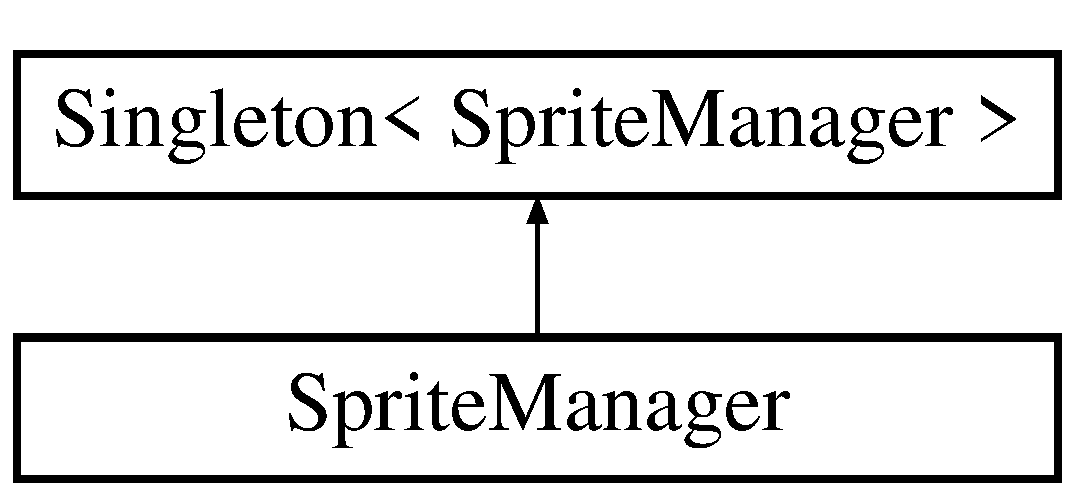
\includegraphics[height=2.000000cm]{class_sprite_manager}
\end{center}
\end{figure}
\subsection*{公開メンバ関数}
\begin{DoxyCompactItemize}
\item 
void \mbox{\hyperlink{class_sprite_manager_a82941ce284548c762f250220ea58f43c}{Init}} ()
\begin{DoxyCompactList}\small\item\em 初期化 \end{DoxyCompactList}\item 
void \mbox{\hyperlink{class_sprite_manager_a5b41702bb7476fb1c148b3e2c81d6b06}{Set\+Texture}} (std\+::string, W\+C\+H\+AR $\ast$)
\begin{DoxyCompactList}\small\item\em テクスチャを保存 \end{DoxyCompactList}\item 
void \mbox{\hyperlink{class_sprite_manager_a4cdd5540bace32d5742ea4df648d87e9}{Render}} (const \mbox{\hyperlink{class_transform}{Transform}} \&, bool, bool, const std\+::string \&, const Direct\+X\+::\+X\+M\+V\+E\+C\+T\+OR \&, const R\+E\+CT \&, const Direct\+X\+::\+Sprite\+Effects)
\begin{DoxyCompactList}\small\item\em 描画 \end{DoxyCompactList}\item 
\mbox{\hyperlink{class_sprite_manager_ae01a31b1c80f676604ba55c93b499e1f}{$\sim$\+Sprite\+Manager}} ()
\begin{DoxyCompactList}\small\item\em デストラクタ \end{DoxyCompactList}\item 
std\+::unique\+\_\+ptr$<$ Direct\+X\+::\+Sprite\+Batch $>$ \& \mbox{\hyperlink{class_sprite_manager_a0b82bacf33d0b558657c8e9841daf9d9}{Get\+Sprite\+Batch}} ()
\begin{DoxyCompactList}\small\item\em Sprite\+Batchのゲッタ \end{DoxyCompactList}\item 
I\+D3\+D11\+Device $\ast$\& \mbox{\hyperlink{class_sprite_manager_ac9e2c44cc43775d9802612bd4be9bac3}{Get\+Device}} ()
\begin{DoxyCompactList}\small\item\em I\+D3\+D11\+Deviceのゲッタ \end{DoxyCompactList}\item 
I\+D3\+D11\+Device\+Context $\ast$\& \mbox{\hyperlink{class_sprite_manager_a6bad23e380818dbe6b521adc07ab84fa}{Get\+Device\+Context}} ()
\begin{DoxyCompactList}\small\item\em I\+D3\+D11\+Device\+Contextのゲッタ \end{DoxyCompactList}\item 
void \mbox{\hyperlink{class_sprite_manager_a6b387e8736713264f6d590082cd492cb}{Start}} ()
\begin{DoxyCompactList}\small\item\em 描画をスタート \end{DoxyCompactList}\item 
void \mbox{\hyperlink{class_sprite_manager_afed8a96a6530f67123a4efa1b6d77032}{End}} ()
\begin{DoxyCompactList}\small\item\em 描画を終了 \end{DoxyCompactList}\end{DoxyCompactItemize}
\subsection*{その他の継承メンバ}


\subsection{詳解}
Sprite関係のデバイスや描画時に経由するものを管理するクラス 

\subsection{構築子と解体子}
\mbox{\Hypertarget{class_sprite_manager_ae01a31b1c80f676604ba55c93b499e1f}\label{class_sprite_manager_ae01a31b1c80f676604ba55c93b499e1f}} 
\index{Sprite\+Manager@{Sprite\+Manager}!````~Sprite\+Manager@{$\sim$\+Sprite\+Manager}}
\index{````~Sprite\+Manager@{$\sim$\+Sprite\+Manager}!Sprite\+Manager@{Sprite\+Manager}}
\subsubsection{\texorpdfstring{$\sim$\+Sprite\+Manager()}{~SpriteManager()}}
{\footnotesize\ttfamily Sprite\+Manager\+::$\sim$\+Sprite\+Manager (\begin{DoxyParamCaption}{ }\end{DoxyParamCaption})}



デストラクタ 



\subsection{関数詳解}
\mbox{\Hypertarget{class_sprite_manager_afed8a96a6530f67123a4efa1b6d77032}\label{class_sprite_manager_afed8a96a6530f67123a4efa1b6d77032}} 
\index{Sprite\+Manager@{Sprite\+Manager}!End@{End}}
\index{End@{End}!Sprite\+Manager@{Sprite\+Manager}}
\subsubsection{\texorpdfstring{End()}{End()}}
{\footnotesize\ttfamily void Sprite\+Manager\+::\+End (\begin{DoxyParamCaption}{ }\end{DoxyParamCaption})\hspace{0.3cm}{\ttfamily [inline]}}



描画を終了 

\mbox{\Hypertarget{class_sprite_manager_ac9e2c44cc43775d9802612bd4be9bac3}\label{class_sprite_manager_ac9e2c44cc43775d9802612bd4be9bac3}} 
\index{Sprite\+Manager@{Sprite\+Manager}!Get\+Device@{Get\+Device}}
\index{Get\+Device@{Get\+Device}!Sprite\+Manager@{Sprite\+Manager}}
\subsubsection{\texorpdfstring{Get\+Device()}{GetDevice()}}
{\footnotesize\ttfamily I\+D3\+D11\+Device$\ast$\& Sprite\+Manager\+::\+Get\+Device (\begin{DoxyParamCaption}{ }\end{DoxyParamCaption})\hspace{0.3cm}{\ttfamily [inline]}}



I\+D3\+D11\+Deviceのゲッタ 

\begin{DoxyReturn}{戻り値}
I\+D3\+D11\+Device$\ast$\& 
\end{DoxyReturn}
\mbox{\Hypertarget{class_sprite_manager_a6bad23e380818dbe6b521adc07ab84fa}\label{class_sprite_manager_a6bad23e380818dbe6b521adc07ab84fa}} 
\index{Sprite\+Manager@{Sprite\+Manager}!Get\+Device\+Context@{Get\+Device\+Context}}
\index{Get\+Device\+Context@{Get\+Device\+Context}!Sprite\+Manager@{Sprite\+Manager}}
\subsubsection{\texorpdfstring{Get\+Device\+Context()}{GetDeviceContext()}}
{\footnotesize\ttfamily I\+D3\+D11\+Device\+Context$\ast$\& Sprite\+Manager\+::\+Get\+Device\+Context (\begin{DoxyParamCaption}{ }\end{DoxyParamCaption})\hspace{0.3cm}{\ttfamily [inline]}}



I\+D3\+D11\+Device\+Contextのゲッタ 

\begin{DoxyReturn}{戻り値}
I\+D3\+D11\+Device\+Context$\ast$\& 
\end{DoxyReturn}
\mbox{\Hypertarget{class_sprite_manager_a0b82bacf33d0b558657c8e9841daf9d9}\label{class_sprite_manager_a0b82bacf33d0b558657c8e9841daf9d9}} 
\index{Sprite\+Manager@{Sprite\+Manager}!Get\+Sprite\+Batch@{Get\+Sprite\+Batch}}
\index{Get\+Sprite\+Batch@{Get\+Sprite\+Batch}!Sprite\+Manager@{Sprite\+Manager}}
\subsubsection{\texorpdfstring{Get\+Sprite\+Batch()}{GetSpriteBatch()}}
{\footnotesize\ttfamily std\+::unique\+\_\+ptr$<$Direct\+X\+::\+Sprite\+Batch$>$\& Sprite\+Manager\+::\+Get\+Sprite\+Batch (\begin{DoxyParamCaption}{ }\end{DoxyParamCaption})\hspace{0.3cm}{\ttfamily [inline]}}



Sprite\+Batchのゲッタ 

\begin{DoxyReturn}{戻り値}
std\+::unique\+\_\+ptr$<$\+Direct\+X\+::\+Sprite\+Batch$>$\& 
\end{DoxyReturn}
\mbox{\Hypertarget{class_sprite_manager_a82941ce284548c762f250220ea58f43c}\label{class_sprite_manager_a82941ce284548c762f250220ea58f43c}} 
\index{Sprite\+Manager@{Sprite\+Manager}!Init@{Init}}
\index{Init@{Init}!Sprite\+Manager@{Sprite\+Manager}}
\subsubsection{\texorpdfstring{Init()}{Init()}}
{\footnotesize\ttfamily void Sprite\+Manager\+::\+Init (\begin{DoxyParamCaption}{ }\end{DoxyParamCaption})}



初期化 

\mbox{\Hypertarget{class_sprite_manager_a4cdd5540bace32d5742ea4df648d87e9}\label{class_sprite_manager_a4cdd5540bace32d5742ea4df648d87e9}} 
\index{Sprite\+Manager@{Sprite\+Manager}!Render@{Render}}
\index{Render@{Render}!Sprite\+Manager@{Sprite\+Manager}}
\subsubsection{\texorpdfstring{Render()}{Render()}}
{\footnotesize\ttfamily void Sprite\+Manager\+::\+Render (\begin{DoxyParamCaption}\item[{const \mbox{\hyperlink{class_transform}{Transform}} \&}]{transform,  }\item[{bool}]{affected\+\_\+camera,  }\item[{bool}]{center\+\_\+axis,  }\item[{const std\+::string \&}]{name,  }\item[{const Direct\+X\+::\+X\+M\+V\+E\+C\+T\+OR \&}]{color,  }\item[{const R\+E\+CT \&}]{rect,  }\item[{const Direct\+X\+::\+Sprite\+Effects}]{sprite\+\_\+effect }\end{DoxyParamCaption})}



描画 


\begin{DoxyParams}{引数}
{\em transform} & 位置や回転、拡大・縮小等 \\
\hline
{\em affected\+\_\+camera} & カメラの影響を受けるかどうか \\
\hline
{\em center\+\_\+axis} & センターを軸にするかどうか \\
\hline
{\em name} & キー \\
\hline
{\em color} & 色 \\
\hline
{\em rect} & テクスチャのどこを描画するかどうか \\
\hline
{\em sprite\+\_\+effect} & 様々の方向の反転 \\
\hline
\end{DoxyParams}
\mbox{\Hypertarget{class_sprite_manager_a5b41702bb7476fb1c148b3e2c81d6b06}\label{class_sprite_manager_a5b41702bb7476fb1c148b3e2c81d6b06}} 
\index{Sprite\+Manager@{Sprite\+Manager}!Set\+Texture@{Set\+Texture}}
\index{Set\+Texture@{Set\+Texture}!Sprite\+Manager@{Sprite\+Manager}}
\subsubsection{\texorpdfstring{Set\+Texture()}{SetTexture()}}
{\footnotesize\ttfamily void Sprite\+Manager\+::\+Set\+Texture (\begin{DoxyParamCaption}\item[{std\+::string}]{name,  }\item[{W\+C\+H\+AR $\ast$}]{path }\end{DoxyParamCaption})}



テクスチャを保存 


\begin{DoxyParams}{引数}
{\em name} & mapで管理するためのキー \\
\hline
{\em path} & テクスチャがあるパス \\
\hline
\end{DoxyParams}
\mbox{\Hypertarget{class_sprite_manager_a6b387e8736713264f6d590082cd492cb}\label{class_sprite_manager_a6b387e8736713264f6d590082cd492cb}} 
\index{Sprite\+Manager@{Sprite\+Manager}!Start@{Start}}
\index{Start@{Start}!Sprite\+Manager@{Sprite\+Manager}}
\subsubsection{\texorpdfstring{Start()}{Start()}}
{\footnotesize\ttfamily void Sprite\+Manager\+::\+Start (\begin{DoxyParamCaption}{ }\end{DoxyParamCaption})\hspace{0.3cm}{\ttfamily [inline]}}



描画をスタート 



このクラス詳解は次のファイルから抽出されました\+:\begin{DoxyCompactItemize}
\item 
C\+:/\+Users/tokir/\+Documents/\+Git\+Hub/\+Weapon\+Merchant\+Adventure/src/rendering/sprite/manager/\mbox{\hyperlink{sprite__manager_8h}{sprite\+\_\+manager.\+h}}\item 
C\+:/\+Users/tokir/\+Documents/\+Git\+Hub/\+Weapon\+Merchant\+Adventure/src/rendering/sprite/manager/\mbox{\hyperlink{sprite__manager_8cpp}{sprite\+\_\+manager.\+cpp}}\end{DoxyCompactItemize}

\hypertarget{class_square_collider}{}\section{Square\+Collider クラス}
\label{class_square_collider}\index{Square\+Collider@{Square\+Collider}}


四角形コライダクラス  




{\ttfamily \#include $<$square\+\_\+collider.\+h$>$}

Square\+Collider の継承関係図\begin{figure}[H]
\begin{center}
\leavevmode
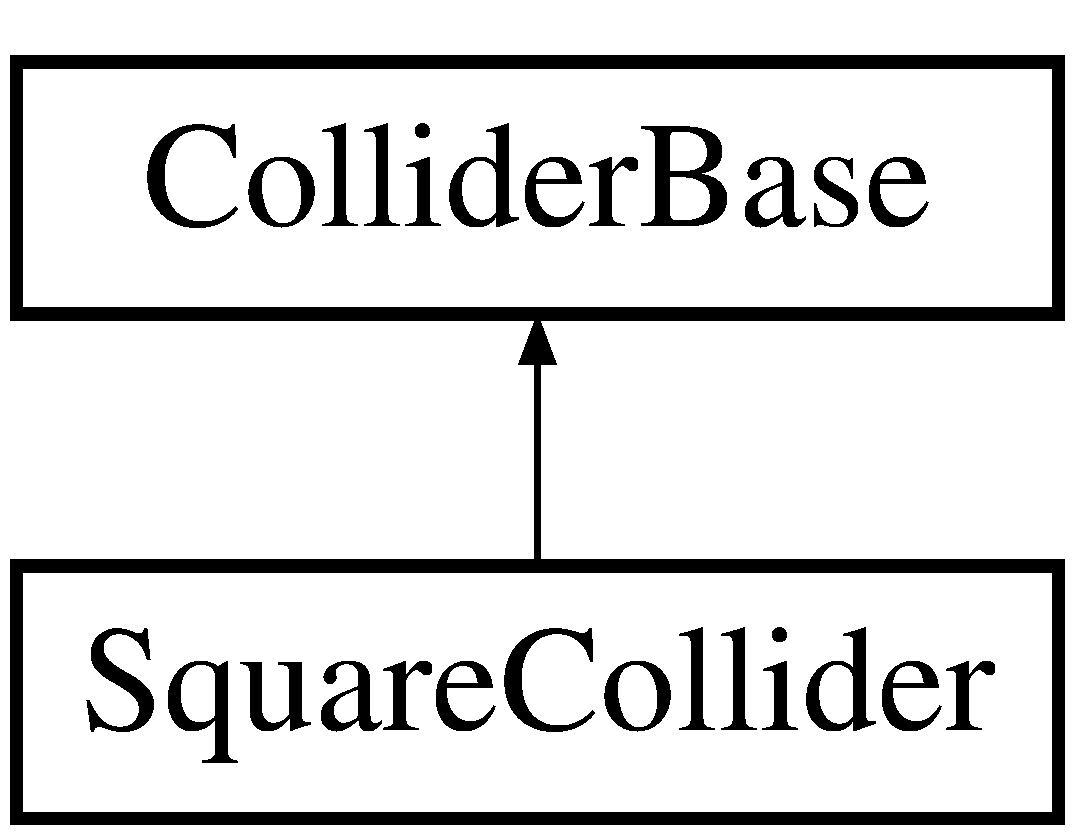
\includegraphics[height=2.000000cm]{class_square_collider}
\end{center}
\end{figure}
\subsection*{公開メンバ関数}
\begin{DoxyCompactItemize}
\item 
\mbox{\hyperlink{class_square_collider_a354753b61e7fa39cb5e7aadcddb78910}{Square\+Collider}} (\mbox{\hyperlink{class_object_base}{Object\+Base}} $\ast$, bool=false, bool=false)
\begin{DoxyCompactList}\small\item\em コンストラクタ \end{DoxyCompactList}\item 
void \mbox{\hyperlink{class_square_collider_a382870e5f0bc29b4f38eb476ecb2fd68}{Set\+Status}} (const \mbox{\hyperlink{common_8h_ab1cb35b3a17c398d8ef71d5f779808bf}{Vec3}} \&pos, const float w, const float h, const \mbox{\hyperlink{common_8h_ab1cb35b3a17c398d8ef71d5f779808bf}{Vec3}} \&scale)
\begin{DoxyCompactList}\small\item\em 当たり判定のステータスをセットする \end{DoxyCompactList}\item 
void \mbox{\hyperlink{class_square_collider_ac250db865d0755fc8731f1660397943d}{Collision\+Extrusion}} (const \mbox{\hyperlink{common_8h_ae148fff5818e9444b4ab2288829559bf}{Vec2}} \&)
\begin{DoxyCompactList}\small\item\em 当たったときの押し出し \end{DoxyCompactList}\item 
const Square\+Status \& \mbox{\hyperlink{class_square_collider_ac437bc1bed951c82ca25d2b17a7b2e0f}{Get\+Status}} () const
\begin{DoxyCompactList}\small\item\em 当たり判定のステータスを返す \end{DoxyCompactList}\item 
void \mbox{\hyperlink{class_square_collider_a83273e0e63692aa8020b8deedd456886}{Destroy}} ()
\begin{DoxyCompactList}\small\item\em 四角形のコライダの破棄 \end{DoxyCompactList}\item 
\mbox{\hyperlink{class_square_collider}{Square\+Collider}} \& \mbox{\hyperlink{class_square_collider_aaa648559b58219a455333f3a100c1d67}{operator=}} (const \mbox{\hyperlink{class_square_collider}{Square\+Collider}} \&other)
\begin{DoxyCompactList}\small\item\em コピー代入演算子 \end{DoxyCompactList}\end{DoxyCompactItemize}
\subsection*{その他の継承メンバ}


\subsection{詳解}
四角形コライダクラス 

\subsection{構築子と解体子}
\mbox{\Hypertarget{class_square_collider_a354753b61e7fa39cb5e7aadcddb78910}\label{class_square_collider_a354753b61e7fa39cb5e7aadcddb78910}} 
\index{Square\+Collider@{Square\+Collider}!Square\+Collider@{Square\+Collider}}
\index{Square\+Collider@{Square\+Collider}!Square\+Collider@{Square\+Collider}}
\subsubsection{\texorpdfstring{Square\+Collider()}{SquareCollider()}}
{\footnotesize\ttfamily Square\+Collider\+::\+Square\+Collider (\begin{DoxyParamCaption}\item[{\mbox{\hyperlink{class_object_base}{Object\+Base}} $\ast$}]{obj,  }\item[{bool}]{\+\_\+is\+\_\+trigger = {\ttfamily false},  }\item[{bool}]{\+\_\+is\+\_\+static = {\ttfamily false} }\end{DoxyParamCaption})}



コンストラクタ 


\begin{DoxyParams}{引数}
{\em obj} & オブジェクト \\
\hline
{\em \+\_\+is\+\_\+trigger} & 当たったときに透けるかどうか \\
\hline
{\em \+\_\+is\+\_\+static} & 静的かどうか \\
\hline
\end{DoxyParams}


\subsection{関数詳解}
\mbox{\Hypertarget{class_square_collider_ac250db865d0755fc8731f1660397943d}\label{class_square_collider_ac250db865d0755fc8731f1660397943d}} 
\index{Square\+Collider@{Square\+Collider}!Collision\+Extrusion@{Collision\+Extrusion}}
\index{Collision\+Extrusion@{Collision\+Extrusion}!Square\+Collider@{Square\+Collider}}
\subsubsection{\texorpdfstring{Collision\+Extrusion()}{CollisionExtrusion()}}
{\footnotesize\ttfamily void Square\+Collider\+::\+Collision\+Extrusion (\begin{DoxyParamCaption}\item[{const \mbox{\hyperlink{common_8h_ae148fff5818e9444b4ab2288829559bf}{Vec2}} \&}]{pos }\end{DoxyParamCaption})}



当たったときの押し出し 


\begin{DoxyParams}{引数}
{\em pos} & 移動先\\
\hline
\end{DoxyParams}
加算減算にしない理由はfloatの誤差が起きてバグらないようにするため \mbox{\Hypertarget{class_square_collider_a83273e0e63692aa8020b8deedd456886}\label{class_square_collider_a83273e0e63692aa8020b8deedd456886}} 
\index{Square\+Collider@{Square\+Collider}!Destroy@{Destroy}}
\index{Destroy@{Destroy}!Square\+Collider@{Square\+Collider}}
\subsubsection{\texorpdfstring{Destroy()}{Destroy()}}
{\footnotesize\ttfamily void Square\+Collider\+::\+Destroy (\begin{DoxyParamCaption}{ }\end{DoxyParamCaption})}



四角形のコライダの破棄 

\mbox{\Hypertarget{class_square_collider_ac437bc1bed951c82ca25d2b17a7b2e0f}\label{class_square_collider_ac437bc1bed951c82ca25d2b17a7b2e0f}} 
\index{Square\+Collider@{Square\+Collider}!Get\+Status@{Get\+Status}}
\index{Get\+Status@{Get\+Status}!Square\+Collider@{Square\+Collider}}
\subsubsection{\texorpdfstring{Get\+Status()}{GetStatus()}}
{\footnotesize\ttfamily const Square\+Status\& Square\+Collider\+::\+Get\+Status (\begin{DoxyParamCaption}{ }\end{DoxyParamCaption}) const\hspace{0.3cm}{\ttfamily [inline]}}



当たり判定のステータスを返す 

\begin{DoxyReturn}{戻り値}
const Square\+Status\& ステータス 
\end{DoxyReturn}
\mbox{\Hypertarget{class_square_collider_aaa648559b58219a455333f3a100c1d67}\label{class_square_collider_aaa648559b58219a455333f3a100c1d67}} 
\index{Square\+Collider@{Square\+Collider}!operator=@{operator=}}
\index{operator=@{operator=}!Square\+Collider@{Square\+Collider}}
\subsubsection{\texorpdfstring{operator=()}{operator=()}}
{\footnotesize\ttfamily \mbox{\hyperlink{class_square_collider}{Square\+Collider}} \& Square\+Collider\+::operator= (\begin{DoxyParamCaption}\item[{const \mbox{\hyperlink{class_square_collider}{Square\+Collider}} \&}]{other }\end{DoxyParamCaption})}



コピー代入演算子 

\mbox{\Hypertarget{class_square_collider_a382870e5f0bc29b4f38eb476ecb2fd68}\label{class_square_collider_a382870e5f0bc29b4f38eb476ecb2fd68}} 
\index{Square\+Collider@{Square\+Collider}!Set\+Status@{Set\+Status}}
\index{Set\+Status@{Set\+Status}!Square\+Collider@{Square\+Collider}}
\subsubsection{\texorpdfstring{Set\+Status()}{SetStatus()}}
{\footnotesize\ttfamily void Square\+Collider\+::\+Set\+Status (\begin{DoxyParamCaption}\item[{const \mbox{\hyperlink{common_8h_ab1cb35b3a17c398d8ef71d5f779808bf}{Vec3}} \&}]{pos,  }\item[{const float}]{w,  }\item[{const float}]{h,  }\item[{const \mbox{\hyperlink{common_8h_ab1cb35b3a17c398d8ef71d5f779808bf}{Vec3}} \&}]{scale }\end{DoxyParamCaption})}



当たり判定のステータスをセットする 


\begin{DoxyParams}{引数}
{\em pos} & センターの位置 \\
\hline
{\em w,h} & 幅、高さ \\
\hline
{\em scale} & 拡大・縮小 \\
\hline
\end{DoxyParams}


このクラス詳解は次のファイルから抽出されました\+:\begin{DoxyCompactItemize}
\item 
C\+:/\+Users/tokir/\+Documents/\+Git\+Hub/\+Weapon\+Merchant\+Adventure/src/src/collider/square/\mbox{\hyperlink{square__collider_8h}{square\+\_\+collider.\+h}}\item 
C\+:/\+Users/tokir/\+Documents/\+Git\+Hub/\+Weapon\+Merchant\+Adventure/src/src/collider/square/\mbox{\hyperlink{square__collider_8cpp}{square\+\_\+collider.\+cpp}}\end{DoxyCompactItemize}

\hypertarget{class_static_object}{}\section{Static\+Object クラス}
\label{class_static_object}\index{Static\+Object@{Static\+Object}}


動かないオブジェクトのスーパークラス  




{\ttfamily \#include $<$static\+\_\+object.\+h$>$}

Static\+Object の継承関係図\begin{figure}[H]
\begin{center}
\leavevmode
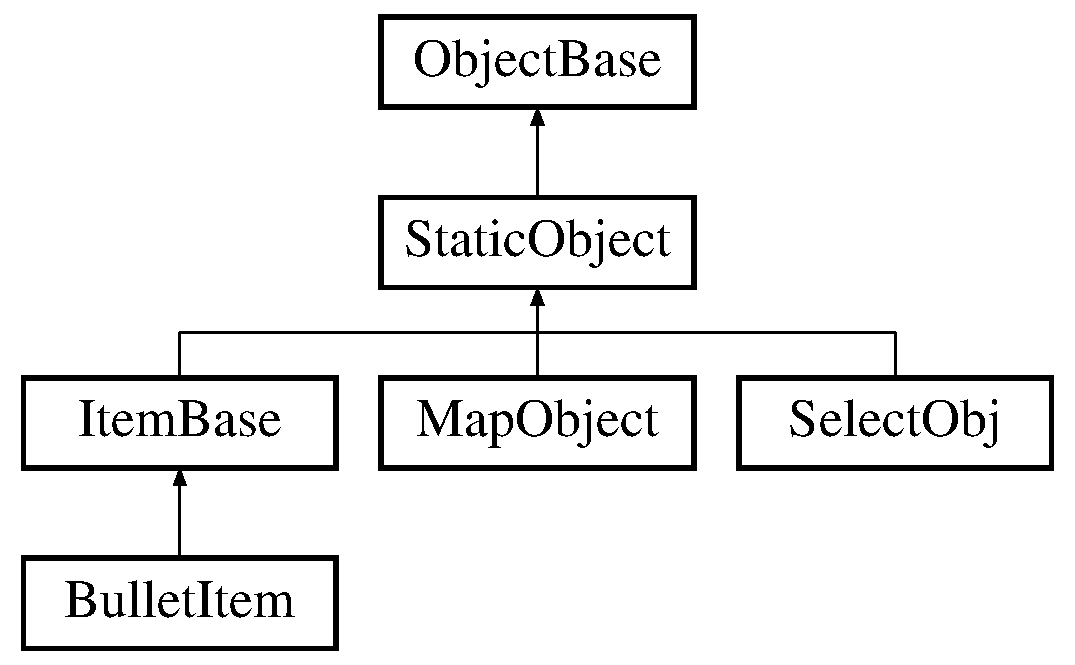
\includegraphics[height=4.000000cm]{class_static_object}
\end{center}
\end{figure}
\subsection*{公開メンバ関数}
\begin{DoxyCompactItemize}
\item 
\mbox{\hyperlink{class_static_object_a2a8e918ddfe5c6723b88b9f5c4156472}{Static\+Object}} ()
\begin{DoxyCompactList}\small\item\em コンストラクタ \end{DoxyCompactList}\item 
\mbox{\hyperlink{class_static_object_a0e1518e656ce5ba408cb69f14ee3066b}{Static\+Object}} (const \mbox{\hyperlink{class_static_object}{Static\+Object}} \&other)
\item 
\mbox{\hyperlink{class_static_object}{Static\+Object}} \& \mbox{\hyperlink{class_static_object_aa2a0526bd19e479ea4d1e5da236c1bf3}{operator=}} (const \mbox{\hyperlink{class_static_object}{Static\+Object}} \&other)
\begin{DoxyCompactList}\small\item\em コピー代入演算子 \end{DoxyCompactList}\item 
virtual void \mbox{\hyperlink{class_static_object_a8e9fb321b4f8f12c4bec1bc66853512f}{Destroy}} ()
\item 
virtual void \mbox{\hyperlink{class_static_object_a64c8803ff881d578d103413e299dbf7f}{Collision}} (\mbox{\hyperlink{class_object_base}{Object\+Base}} $\ast$, \mbox{\hyperlink{common_8h_ae148fff5818e9444b4ab2288829559bf}{Vec2}})
\item 
virtual \mbox{\hyperlink{class_static_object_ac27301fc3d8d22aff5664f592c375cd8}{$\sim$\+Static\+Object}} ()
\item 
void \mbox{\hyperlink{class_static_object_a44408a8130d19f7284fe4daaab87c712}{Set\+Color}} (const float, const float, const float, const float)
\end{DoxyCompactItemize}
\subsection*{限定公開メンバ関数}
\begin{DoxyCompactItemize}
\item 
void \mbox{\hyperlink{class_static_object_afec57009537695c4715386120a619942}{Render\+Process}} (bool)
\begin{DoxyCompactList}\small\item\em 描画 \end{DoxyCompactList}\item 
virtual void \mbox{\hyperlink{class_static_object_afa0709f50495338a23c1140062a567af}{Init\+Process}} ()
\item 
virtual void \mbox{\hyperlink{class_static_object_a7fa678c3c4032bb6e9417f93a8bb895c}{Update\+Process}} ()
\item 
virtual void \mbox{\hyperlink{class_static_object_a36379eb74b66c1586f1cc678a85c52c1}{Collision\+Process}} (\mbox{\hyperlink{class_object_base}{Object\+Base}} $\ast$, \mbox{\hyperlink{common_8h_ae148fff5818e9444b4ab2288829559bf}{Vec2}})
\end{DoxyCompactItemize}
\subsection*{その他の継承メンバ}


\subsection{詳解}
動かないオブジェクトのスーパークラス 

\subsection{構築子と解体子}
\mbox{\Hypertarget{class_static_object_a2a8e918ddfe5c6723b88b9f5c4156472}\label{class_static_object_a2a8e918ddfe5c6723b88b9f5c4156472}} 
\index{Static\+Object@{Static\+Object}!Static\+Object@{Static\+Object}}
\index{Static\+Object@{Static\+Object}!Static\+Object@{Static\+Object}}
\subsubsection{\texorpdfstring{Static\+Object()}{StaticObject()}\hspace{0.1cm}{\footnotesize\ttfamily [1/2]}}
{\footnotesize\ttfamily Static\+Object\+::\+Static\+Object (\begin{DoxyParamCaption}{ }\end{DoxyParamCaption})\hspace{0.3cm}{\ttfamily [inline]}}



コンストラクタ 

\mbox{\Hypertarget{class_static_object_a0e1518e656ce5ba408cb69f14ee3066b}\label{class_static_object_a0e1518e656ce5ba408cb69f14ee3066b}} 
\index{Static\+Object@{Static\+Object}!Static\+Object@{Static\+Object}}
\index{Static\+Object@{Static\+Object}!Static\+Object@{Static\+Object}}
\subsubsection{\texorpdfstring{Static\+Object()}{StaticObject()}\hspace{0.1cm}{\footnotesize\ttfamily [2/2]}}
{\footnotesize\ttfamily Static\+Object\+::\+Static\+Object (\begin{DoxyParamCaption}\item[{const \mbox{\hyperlink{class_static_object}{Static\+Object}} \&}]{other }\end{DoxyParamCaption})\hspace{0.3cm}{\ttfamily [inline]}}

\mbox{\Hypertarget{class_static_object_ac27301fc3d8d22aff5664f592c375cd8}\label{class_static_object_ac27301fc3d8d22aff5664f592c375cd8}} 
\index{Static\+Object@{Static\+Object}!````~Static\+Object@{$\sim$\+Static\+Object}}
\index{````~Static\+Object@{$\sim$\+Static\+Object}!Static\+Object@{Static\+Object}}
\subsubsection{\texorpdfstring{$\sim$\+Static\+Object()}{~StaticObject()}}
{\footnotesize\ttfamily virtual Static\+Object\+::$\sim$\+Static\+Object (\begin{DoxyParamCaption}{ }\end{DoxyParamCaption})\hspace{0.3cm}{\ttfamily [inline]}, {\ttfamily [virtual]}}



\subsection{関数詳解}
\mbox{\Hypertarget{class_static_object_a64c8803ff881d578d103413e299dbf7f}\label{class_static_object_a64c8803ff881d578d103413e299dbf7f}} 
\index{Static\+Object@{Static\+Object}!Collision@{Collision}}
\index{Collision@{Collision}!Static\+Object@{Static\+Object}}
\subsubsection{\texorpdfstring{Collision()}{Collision()}}
{\footnotesize\ttfamily virtual void Static\+Object\+::\+Collision (\begin{DoxyParamCaption}\item[{\mbox{\hyperlink{class_object_base}{Object\+Base}} $\ast$}]{,  }\item[{\mbox{\hyperlink{common_8h_ae148fff5818e9444b4ab2288829559bf}{Vec2}}}]{ }\end{DoxyParamCaption})\hspace{0.3cm}{\ttfamily [inline]}, {\ttfamily [virtual]}}



\mbox{\hyperlink{class_object_base_a3e1db79dfa119be067d816c22d09839d}{Object\+Base}}を再実装しています。



\mbox{\hyperlink{class_item_base_ae5c2bcf78c74126a6f76783ca927c7ab}{Item\+Base}}, \mbox{\hyperlink{class_map_object_a76b9161f2723272ad361d0b190e46245}{Map\+Object}}, \mbox{\hyperlink{class_select_obj_a497ff683aefe9bf77201eee1e3948e15}{Select\+Obj}}で再実装されています。

\mbox{\Hypertarget{class_static_object_a36379eb74b66c1586f1cc678a85c52c1}\label{class_static_object_a36379eb74b66c1586f1cc678a85c52c1}} 
\index{Static\+Object@{Static\+Object}!Collision\+Process@{Collision\+Process}}
\index{Collision\+Process@{Collision\+Process}!Static\+Object@{Static\+Object}}
\subsubsection{\texorpdfstring{Collision\+Process()}{CollisionProcess()}}
{\footnotesize\ttfamily virtual void Static\+Object\+::\+Collision\+Process (\begin{DoxyParamCaption}\item[{\mbox{\hyperlink{class_object_base}{Object\+Base}} $\ast$}]{,  }\item[{\mbox{\hyperlink{common_8h_ae148fff5818e9444b4ab2288829559bf}{Vec2}}}]{ }\end{DoxyParamCaption})\hspace{0.3cm}{\ttfamily [inline]}, {\ttfamily [protected]}, {\ttfamily [virtual]}}

\mbox{\Hypertarget{class_static_object_a8e9fb321b4f8f12c4bec1bc66853512f}\label{class_static_object_a8e9fb321b4f8f12c4bec1bc66853512f}} 
\index{Static\+Object@{Static\+Object}!Destroy@{Destroy}}
\index{Destroy@{Destroy}!Static\+Object@{Static\+Object}}
\subsubsection{\texorpdfstring{Destroy()}{Destroy()}}
{\footnotesize\ttfamily virtual void Static\+Object\+::\+Destroy (\begin{DoxyParamCaption}{ }\end{DoxyParamCaption})\hspace{0.3cm}{\ttfamily [inline]}, {\ttfamily [virtual]}}



\mbox{\hyperlink{class_object_base_a7fa4c548153c3af20f89673ffea809af}{Object\+Base}}を実装しています。



\mbox{\hyperlink{class_map_object_ad4bcfdc33bd945a9aa5e50a57c2704bc}{Map\+Object}}, \mbox{\hyperlink{class_item_base_ab34d53b8f3442da77466ba1b9132386e}{Item\+Base}}, \mbox{\hyperlink{class_select_obj_ad3a5fdc41a9e5753f99bae7ad289888f}{Select\+Obj}}で再実装されています。

\mbox{\Hypertarget{class_static_object_afa0709f50495338a23c1140062a567af}\label{class_static_object_afa0709f50495338a23c1140062a567af}} 
\index{Static\+Object@{Static\+Object}!Init\+Process@{Init\+Process}}
\index{Init\+Process@{Init\+Process}!Static\+Object@{Static\+Object}}
\subsubsection{\texorpdfstring{Init\+Process()}{InitProcess()}}
{\footnotesize\ttfamily virtual void Static\+Object\+::\+Init\+Process (\begin{DoxyParamCaption}{ }\end{DoxyParamCaption})\hspace{0.3cm}{\ttfamily [inline]}, {\ttfamily [protected]}, {\ttfamily [virtual]}}



\mbox{\hyperlink{class_object_base_af133f36f2bca1dcfd962e2cfac61ab51}{Object\+Base}}を実装しています。



\mbox{\hyperlink{class_map_object_a3043cddb8aaad0eab27a076e9bee0284}{Map\+Object}}, \mbox{\hyperlink{class_select_obj_a09c9e1a54f4605eda5bb6e18887c2654}{Select\+Obj}}, \mbox{\hyperlink{class_item_base_a772804cb3c663b35e44d49913d1f1cef}{Item\+Base}}で再実装されています。

\mbox{\Hypertarget{class_static_object_aa2a0526bd19e479ea4d1e5da236c1bf3}\label{class_static_object_aa2a0526bd19e479ea4d1e5da236c1bf3}} 
\index{Static\+Object@{Static\+Object}!operator=@{operator=}}
\index{operator=@{operator=}!Static\+Object@{Static\+Object}}
\subsubsection{\texorpdfstring{operator=()}{operator=()}}
{\footnotesize\ttfamily \mbox{\hyperlink{class_static_object}{Static\+Object}}\& Static\+Object\+::operator= (\begin{DoxyParamCaption}\item[{const \mbox{\hyperlink{class_static_object}{Static\+Object}} \&}]{other }\end{DoxyParamCaption})\hspace{0.3cm}{\ttfamily [inline]}}



コピー代入演算子 

\mbox{\Hypertarget{class_static_object_afec57009537695c4715386120a619942}\label{class_static_object_afec57009537695c4715386120a619942}} 
\index{Static\+Object@{Static\+Object}!Render\+Process@{Render\+Process}}
\index{Render\+Process@{Render\+Process}!Static\+Object@{Static\+Object}}
\subsubsection{\texorpdfstring{Render\+Process()}{RenderProcess()}}
{\footnotesize\ttfamily void Static\+Object\+::\+Render\+Process (\begin{DoxyParamCaption}\item[{bool}]{camera\+\_\+affected }\end{DoxyParamCaption})\hspace{0.3cm}{\ttfamily [protected]}, {\ttfamily [virtual]}}



描画 


\begin{DoxyParams}{引数}
{\em camera\+\_\+affected} & カメラの位置によって位置を変えるかどうか \\
\hline
\end{DoxyParams}


\mbox{\hyperlink{class_object_base_aeac51d868beeb7f7fe900407b76b93a2}{Object\+Base}}を実装しています。

\mbox{\Hypertarget{class_static_object_a44408a8130d19f7284fe4daaab87c712}\label{class_static_object_a44408a8130d19f7284fe4daaab87c712}} 
\index{Static\+Object@{Static\+Object}!Set\+Color@{Set\+Color}}
\index{Set\+Color@{Set\+Color}!Static\+Object@{Static\+Object}}
\subsubsection{\texorpdfstring{Set\+Color()}{SetColor()}}
{\footnotesize\ttfamily void Static\+Object\+::\+Set\+Color (\begin{DoxyParamCaption}\item[{const float}]{r,  }\item[{const float}]{g,  }\item[{const float}]{b,  }\item[{const float}]{a }\end{DoxyParamCaption})}

\mbox{\Hypertarget{class_static_object_a7fa678c3c4032bb6e9417f93a8bb895c}\label{class_static_object_a7fa678c3c4032bb6e9417f93a8bb895c}} 
\index{Static\+Object@{Static\+Object}!Update\+Process@{Update\+Process}}
\index{Update\+Process@{Update\+Process}!Static\+Object@{Static\+Object}}
\subsubsection{\texorpdfstring{Update\+Process()}{UpdateProcess()}}
{\footnotesize\ttfamily virtual void Static\+Object\+::\+Update\+Process (\begin{DoxyParamCaption}{ }\end{DoxyParamCaption})\hspace{0.3cm}{\ttfamily [inline]}, {\ttfamily [protected]}, {\ttfamily [virtual]}}



\mbox{\hyperlink{class_object_base_a8b5b72b363a419767efde0b0e692ea95}{Object\+Base}}を実装しています。



\mbox{\hyperlink{class_map_object_ab6b8849f15175417eca94b2703945e4b}{Map\+Object}}, \mbox{\hyperlink{class_item_base_a8edff8edcf884f9590f973fd05d218bc}{Item\+Base}}, \mbox{\hyperlink{class_select_obj_a4788d957629f0b69dc78166f09f949bb}{Select\+Obj}}で再実装されています。



このクラス詳解は次のファイルから抽出されました\+:\begin{DoxyCompactItemize}
\item 
C\+:/\+Users/tokir/\+Documents/\+Git\+Hub/\+Weapon\+Merchant\+Adventure/src/src/object/base/static/\mbox{\hyperlink{static__object_8h}{static\+\_\+object.\+h}}\item 
C\+:/\+Users/tokir/\+Documents/\+Git\+Hub/\+Weapon\+Merchant\+Adventure/src/src/object/base/static/\mbox{\hyperlink{static__object_8cpp}{static\+\_\+object.\+cpp}}\end{DoxyCompactItemize}

\hypertarget{class_status}{}\section{Status クラス}
\label{class_status}\index{Status@{Status}}


ステータスクラス  




{\ttfamily \#include $<$status.\+h$>$}

\subsection*{公開メンバ関数}
\begin{DoxyCompactItemize}
\item 
void \mbox{\hyperlink{class_status_a04cf2752224db252d7694c2caf5caf83}{Init}} (const float hp, const float attack, const float defense)
\begin{DoxyCompactList}\small\item\em 初期化 \end{DoxyCompactList}\item 
\mbox{\hyperlink{class_status}{Status}} \& \mbox{\hyperlink{class_status_abc76064ed2504493c3bbc0f287a49525}{operator=}} (const \mbox{\hyperlink{class_status}{Status}} \&other)
\end{DoxyCompactItemize}
\subsection*{公開変数類}
\begin{DoxyCompactItemize}
\item 
float \mbox{\hyperlink{class_status_a0ec54fdb31c6c4b1a23b22742e6babb4}{HP}}
\item 
float \mbox{\hyperlink{class_status_aede601b020ef15845b86d631a46f8980}{Attack}}
\item 
float \mbox{\hyperlink{class_status_aee944c63904ca1b6b3b04e24b2a9ac12}{Defense}}
\end{DoxyCompactItemize}


\subsection{詳解}
ステータスクラス 

\subsection{関数詳解}
\mbox{\Hypertarget{class_status_a04cf2752224db252d7694c2caf5caf83}\label{class_status_a04cf2752224db252d7694c2caf5caf83}} 
\index{Status@{Status}!Init@{Init}}
\index{Init@{Init}!Status@{Status}}
\subsubsection{\texorpdfstring{Init()}{Init()}}
{\footnotesize\ttfamily void Status\+::\+Init (\begin{DoxyParamCaption}\item[{const float}]{hp,  }\item[{const float}]{attack,  }\item[{const float}]{defense }\end{DoxyParamCaption})\hspace{0.3cm}{\ttfamily [inline]}}



初期化 


\begin{DoxyParams}{引数}
{\em hp} & 初期\+HP \\
\hline
{\em attack} & 攻撃力 \\
\hline
{\em defense} & 防御力 \\
\hline
\end{DoxyParams}
\mbox{\Hypertarget{class_status_abc76064ed2504493c3bbc0f287a49525}\label{class_status_abc76064ed2504493c3bbc0f287a49525}} 
\index{Status@{Status}!operator=@{operator=}}
\index{operator=@{operator=}!Status@{Status}}
\subsubsection{\texorpdfstring{operator=()}{operator=()}}
{\footnotesize\ttfamily \mbox{\hyperlink{class_status}{Status}}\& Status\+::operator= (\begin{DoxyParamCaption}\item[{const \mbox{\hyperlink{class_status}{Status}} \&}]{other }\end{DoxyParamCaption})\hspace{0.3cm}{\ttfamily [inline]}}



\subsection{メンバ詳解}
\mbox{\Hypertarget{class_status_aede601b020ef15845b86d631a46f8980}\label{class_status_aede601b020ef15845b86d631a46f8980}} 
\index{Status@{Status}!Attack@{Attack}}
\index{Attack@{Attack}!Status@{Status}}
\subsubsection{\texorpdfstring{Attack}{Attack}}
{\footnotesize\ttfamily float Status\+::\+Attack}

\mbox{\Hypertarget{class_status_aee944c63904ca1b6b3b04e24b2a9ac12}\label{class_status_aee944c63904ca1b6b3b04e24b2a9ac12}} 
\index{Status@{Status}!Defense@{Defense}}
\index{Defense@{Defense}!Status@{Status}}
\subsubsection{\texorpdfstring{Defense}{Defense}}
{\footnotesize\ttfamily float Status\+::\+Defense}

\mbox{\Hypertarget{class_status_a0ec54fdb31c6c4b1a23b22742e6babb4}\label{class_status_a0ec54fdb31c6c4b1a23b22742e6babb4}} 
\index{Status@{Status}!HP@{HP}}
\index{HP@{HP}!Status@{Status}}
\subsubsection{\texorpdfstring{HP}{HP}}
{\footnotesize\ttfamily float Status\+::\+HP}



このクラス詳解は次のファイルから抽出されました\+:\begin{DoxyCompactItemize}
\item 
C\+:/\+Users/tokir/\+Documents/\+Git\+Hub/\+Weapon\+Merchant\+Adventure/src/status/\mbox{\hyperlink{status_8h}{status.\+h}}\end{DoxyCompactItemize}

\hypertarget{class_sword}{}\section{Sword クラス}
\label{class_sword}\index{Sword@{Sword}}


剣クラス  




{\ttfamily \#include $<$sword.\+h$>$}

Sword の継承関係図\begin{figure}[H]
\begin{center}
\leavevmode
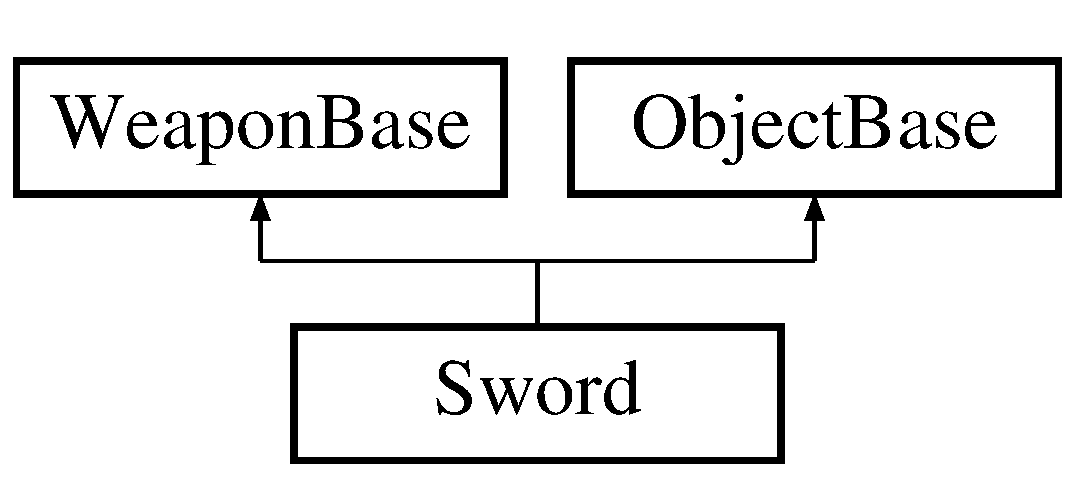
\includegraphics[height=2.000000cm]{class_sword}
\end{center}
\end{figure}
\subsection*{公開メンバ関数}
\begin{DoxyCompactItemize}
\item 
\mbox{\hyperlink{class_sword_af33284e40825ec8ddccd01fa5833be36}{Sword}} ()
\begin{DoxyCompactList}\small\item\em コンストラクタ \end{DoxyCompactList}\item 
\mbox{\hyperlink{class_sword_a6a55d930547584000fcc7c63d47ffabf}{Sword}} (const \mbox{\hyperlink{class_sword}{Sword}} \&s)
\begin{DoxyCompactList}\small\item\em コピーコンストラクタ \end{DoxyCompactList}\item 
\mbox{\hyperlink{class_sword}{Sword}} \& \mbox{\hyperlink{class_sword_a47720cf8f0a44a9a30cf586a188a4730}{operator=}} (const \mbox{\hyperlink{class_sword}{Sword}} \&other)
\begin{DoxyCompactList}\small\item\em 代入演算子 \end{DoxyCompactList}\item 
void \mbox{\hyperlink{class_sword_af9027f627d1db6c0ac21d2aa842cff69}{Weapon\+Start}} () final
\begin{DoxyCompactList}\small\item\em 武器用の初期化 \end{DoxyCompactList}\item 
void \mbox{\hyperlink{class_sword_a5fda2f72829b6256ffc3fb18d9d065e8}{Weapon\+Update}} (const \mbox{\hyperlink{common_8h_ab1cb35b3a17c398d8ef71d5f779808bf}{Vec3}} \&, bool) final
\begin{DoxyCompactList}\small\item\em 武器用の更新 \end{DoxyCompactList}\item 
void \mbox{\hyperlink{class_sword_a3f60d8b24b7847d6a84f0941820b711d}{Weapon\+Destroy}} () final
\begin{DoxyCompactList}\small\item\em 武器用の破棄 \end{DoxyCompactList}\item 
void \mbox{\hyperlink{class_sword_a1dcab625754ca097ad814ee544c6a872}{Collision}} (\mbox{\hyperlink{class_object_base}{Object\+Base}} $\ast$, \mbox{\hyperlink{common_8h_ae148fff5818e9444b4ab2288829559bf}{Vec2}}) final
\begin{DoxyCompactList}\small\item\em 当たったときの反応 \end{DoxyCompactList}\item 
bool \mbox{\hyperlink{class_sword_a6c8642e6a8f1d6152abce6c84bf6d21b}{Attack}} (bool, const \mbox{\hyperlink{common_8h_ab1cb35b3a17c398d8ef71d5f779808bf}{Vec3}} \&) final
\begin{DoxyCompactList}\small\item\em 攻撃 \end{DoxyCompactList}\item 
void \mbox{\hyperlink{class_sword_ac80e3b54ef5572eae1e4760d14383f4f}{Weapon\+Render}} (const \mbox{\hyperlink{common_8h_a1c43cb8f0d8a41901f3ce4c67dbbce20}{Transform}} \&=\mbox{\hyperlink{common_8h_a1c43cb8f0d8a41901f3ce4c67dbbce20}{Transform}}\{ saki\+::vector3\+\_\+zero$<$ float $>$, saki\+::vector3\+\_\+zero$<$ float $>$, saki\+::vector3\+\_\+zero$<$ float $>$ \}) final
\begin{DoxyCompactList}\small\item\em 武器用の描画 \end{DoxyCompactList}\item 
void \mbox{\hyperlink{class_sword_a8473b694775374df4d9b6305cfa82293}{Destroy}} ()
\end{DoxyCompactItemize}
\subsection*{限定公開メンバ関数}
\begin{DoxyCompactItemize}
\item 
void \mbox{\hyperlink{class_sword_a7f5d2c6e6e0104e9a85f600eec14ef6d}{Render\+Process}} (bool) final
\item 
void \mbox{\hyperlink{class_sword_aab0c07888f3aaee1ba25d668ac7c847a}{Init\+Process}} () final
\item 
void \mbox{\hyperlink{class_sword_a3e0221aa5c05ecada9def39fb38c0059}{Update\+Process}} () final
\end{DoxyCompactItemize}
\subsection*{その他の継承メンバ}


\subsection{詳解}
剣クラス 

\subsection{構築子と解体子}
\mbox{\Hypertarget{class_sword_af33284e40825ec8ddccd01fa5833be36}\label{class_sword_af33284e40825ec8ddccd01fa5833be36}} 
\index{Sword@{Sword}!Sword@{Sword}}
\index{Sword@{Sword}!Sword@{Sword}}
\subsubsection{\texorpdfstring{Sword()}{Sword()}\hspace{0.1cm}{\footnotesize\ttfamily [1/2]}}
{\footnotesize\ttfamily Sword\+::\+Sword (\begin{DoxyParamCaption}{ }\end{DoxyParamCaption})}



コンストラクタ 

\mbox{\Hypertarget{class_sword_a6a55d930547584000fcc7c63d47ffabf}\label{class_sword_a6a55d930547584000fcc7c63d47ffabf}} 
\index{Sword@{Sword}!Sword@{Sword}}
\index{Sword@{Sword}!Sword@{Sword}}
\subsubsection{\texorpdfstring{Sword()}{Sword()}\hspace{0.1cm}{\footnotesize\ttfamily [2/2]}}
{\footnotesize\ttfamily Sword\+::\+Sword (\begin{DoxyParamCaption}\item[{const \mbox{\hyperlink{class_sword}{Sword}} \&}]{s }\end{DoxyParamCaption})\hspace{0.3cm}{\ttfamily [inline]}}



コピーコンストラクタ 



\subsection{関数詳解}
\mbox{\Hypertarget{class_sword_a6c8642e6a8f1d6152abce6c84bf6d21b}\label{class_sword_a6c8642e6a8f1d6152abce6c84bf6d21b}} 
\index{Sword@{Sword}!Attack@{Attack}}
\index{Attack@{Attack}!Sword@{Sword}}
\subsubsection{\texorpdfstring{Attack()}{Attack()}}
{\footnotesize\ttfamily bool Sword\+::\+Attack (\begin{DoxyParamCaption}\item[{bool}]{\+\_\+right,  }\item[{const \mbox{\hyperlink{common_8h_ab1cb35b3a17c398d8ef71d5f779808bf}{Vec3}} \&}]{pos }\end{DoxyParamCaption})\hspace{0.3cm}{\ttfamily [final]}, {\ttfamily [virtual]}}



攻撃 


\begin{DoxyParams}{引数}
{\em \+\_\+right} & 右向きかどうか \\
\hline
{\em pos} & 位置 \\
\hline
\end{DoxyParams}


\mbox{\hyperlink{class_weapon_base_a1bab9c7fb9524db754bebbbcbf6c2fd9}{Weapon\+Base}}を実装しています。

\mbox{\Hypertarget{class_sword_a1dcab625754ca097ad814ee544c6a872}\label{class_sword_a1dcab625754ca097ad814ee544c6a872}} 
\index{Sword@{Sword}!Collision@{Collision}}
\index{Collision@{Collision}!Sword@{Sword}}
\subsubsection{\texorpdfstring{Collision()}{Collision()}}
{\footnotesize\ttfamily void Sword\+::\+Collision (\begin{DoxyParamCaption}\item[{\mbox{\hyperlink{class_object_base}{Object\+Base}} $\ast$}]{obj,  }\item[{\mbox{\hyperlink{common_8h_ae148fff5818e9444b4ab2288829559bf}{Vec2}}}]{ }\end{DoxyParamCaption})\hspace{0.3cm}{\ttfamily [final]}, {\ttfamily [virtual]}}



当たったときの反応 


\begin{DoxyParams}{引数}
{\em obj} & 当たった相手のオブジェクト \\
\hline
\end{DoxyParams}


\mbox{\hyperlink{class_object_base_a3e1db79dfa119be067d816c22d09839d}{Object\+Base}}を再実装しています。

\mbox{\Hypertarget{class_sword_a8473b694775374df4d9b6305cfa82293}\label{class_sword_a8473b694775374df4d9b6305cfa82293}} 
\index{Sword@{Sword}!Destroy@{Destroy}}
\index{Destroy@{Destroy}!Sword@{Sword}}
\subsubsection{\texorpdfstring{Destroy()}{Destroy()}}
{\footnotesize\ttfamily void Sword\+::\+Destroy (\begin{DoxyParamCaption}{ }\end{DoxyParamCaption})\hspace{0.3cm}{\ttfamily [inline]}, {\ttfamily [virtual]}}



\mbox{\hyperlink{class_object_base_a7fa4c548153c3af20f89673ffea809af}{Object\+Base}}を実装しています。

\mbox{\Hypertarget{class_sword_aab0c07888f3aaee1ba25d668ac7c847a}\label{class_sword_aab0c07888f3aaee1ba25d668ac7c847a}} 
\index{Sword@{Sword}!Init\+Process@{Init\+Process}}
\index{Init\+Process@{Init\+Process}!Sword@{Sword}}
\subsubsection{\texorpdfstring{Init\+Process()}{InitProcess()}}
{\footnotesize\ttfamily void Sword\+::\+Init\+Process (\begin{DoxyParamCaption}{ }\end{DoxyParamCaption})\hspace{0.3cm}{\ttfamily [inline]}, {\ttfamily [final]}, {\ttfamily [protected]}, {\ttfamily [virtual]}}



\mbox{\hyperlink{class_object_base_af133f36f2bca1dcfd962e2cfac61ab51}{Object\+Base}}を実装しています。

\mbox{\Hypertarget{class_sword_a47720cf8f0a44a9a30cf586a188a4730}\label{class_sword_a47720cf8f0a44a9a30cf586a188a4730}} 
\index{Sword@{Sword}!operator=@{operator=}}
\index{operator=@{operator=}!Sword@{Sword}}
\subsubsection{\texorpdfstring{operator=()}{operator=()}}
{\footnotesize\ttfamily \mbox{\hyperlink{class_sword}{Sword}}\& Sword\+::operator= (\begin{DoxyParamCaption}\item[{const \mbox{\hyperlink{class_sword}{Sword}} \&}]{other }\end{DoxyParamCaption})\hspace{0.3cm}{\ttfamily [inline]}}



代入演算子 

\mbox{\Hypertarget{class_sword_a7f5d2c6e6e0104e9a85f600eec14ef6d}\label{class_sword_a7f5d2c6e6e0104e9a85f600eec14ef6d}} 
\index{Sword@{Sword}!Render\+Process@{Render\+Process}}
\index{Render\+Process@{Render\+Process}!Sword@{Sword}}
\subsubsection{\texorpdfstring{Render\+Process()}{RenderProcess()}}
{\footnotesize\ttfamily void Sword\+::\+Render\+Process (\begin{DoxyParamCaption}\item[{bool}]{ }\end{DoxyParamCaption})\hspace{0.3cm}{\ttfamily [inline]}, {\ttfamily [final]}, {\ttfamily [protected]}, {\ttfamily [virtual]}}



\mbox{\hyperlink{class_object_base_aeac51d868beeb7f7fe900407b76b93a2}{Object\+Base}}を実装しています。

\mbox{\Hypertarget{class_sword_a3e0221aa5c05ecada9def39fb38c0059}\label{class_sword_a3e0221aa5c05ecada9def39fb38c0059}} 
\index{Sword@{Sword}!Update\+Process@{Update\+Process}}
\index{Update\+Process@{Update\+Process}!Sword@{Sword}}
\subsubsection{\texorpdfstring{Update\+Process()}{UpdateProcess()}}
{\footnotesize\ttfamily void Sword\+::\+Update\+Process (\begin{DoxyParamCaption}{ }\end{DoxyParamCaption})\hspace{0.3cm}{\ttfamily [inline]}, {\ttfamily [final]}, {\ttfamily [protected]}, {\ttfamily [virtual]}}



\mbox{\hyperlink{class_object_base_a8b5b72b363a419767efde0b0e692ea95}{Object\+Base}}を実装しています。

\mbox{\Hypertarget{class_sword_a3f60d8b24b7847d6a84f0941820b711d}\label{class_sword_a3f60d8b24b7847d6a84f0941820b711d}} 
\index{Sword@{Sword}!Weapon\+Destroy@{Weapon\+Destroy}}
\index{Weapon\+Destroy@{Weapon\+Destroy}!Sword@{Sword}}
\subsubsection{\texorpdfstring{Weapon\+Destroy()}{WeaponDestroy()}}
{\footnotesize\ttfamily void Sword\+::\+Weapon\+Destroy (\begin{DoxyParamCaption}{ }\end{DoxyParamCaption})\hspace{0.3cm}{\ttfamily [final]}, {\ttfamily [virtual]}}



武器用の破棄 



\mbox{\hyperlink{class_weapon_base_a417784a8c8bf73cd398a77b922fc110c}{Weapon\+Base}}を実装しています。

\mbox{\Hypertarget{class_sword_ac80e3b54ef5572eae1e4760d14383f4f}\label{class_sword_ac80e3b54ef5572eae1e4760d14383f4f}} 
\index{Sword@{Sword}!Weapon\+Render@{Weapon\+Render}}
\index{Weapon\+Render@{Weapon\+Render}!Sword@{Sword}}
\subsubsection{\texorpdfstring{Weapon\+Render()}{WeaponRender()}}
{\footnotesize\ttfamily void Sword\+::\+Weapon\+Render (\begin{DoxyParamCaption}\item[{const \mbox{\hyperlink{common_8h_a1c43cb8f0d8a41901f3ce4c67dbbce20}{Transform}} \&}]{ = {\ttfamily \mbox{\hyperlink{common_8h_a1c43cb8f0d8a41901f3ce4c67dbbce20}{Transform}}\{~saki\+:\+:vector3\+\_\+zero$<$float$>$,saki\+:\+:vector3\+\_\+zero$<$float$>$,saki\+:\+:vector3\+\_\+zero$<$float$>$~\}} }\end{DoxyParamCaption})\hspace{0.3cm}{\ttfamily [final]}, {\ttfamily [virtual]}}



武器用の描画 


\begin{DoxyParams}{引数}
{\em t} & 描画位置 \\
\hline
\end{DoxyParams}


\mbox{\hyperlink{class_weapon_base_af308d16d3892c3ffaeedf74b08e761b9}{Weapon\+Base}}を実装しています。

\mbox{\Hypertarget{class_sword_af9027f627d1db6c0ac21d2aa842cff69}\label{class_sword_af9027f627d1db6c0ac21d2aa842cff69}} 
\index{Sword@{Sword}!Weapon\+Start@{Weapon\+Start}}
\index{Weapon\+Start@{Weapon\+Start}!Sword@{Sword}}
\subsubsection{\texorpdfstring{Weapon\+Start()}{WeaponStart()}}
{\footnotesize\ttfamily void Sword\+::\+Weapon\+Start (\begin{DoxyParamCaption}{ }\end{DoxyParamCaption})\hspace{0.3cm}{\ttfamily [final]}, {\ttfamily [virtual]}}



武器用の初期化 



\mbox{\hyperlink{class_weapon_base_a25cd4c351638b76377e93341a9545712}{Weapon\+Base}}を実装しています。

\mbox{\Hypertarget{class_sword_a5fda2f72829b6256ffc3fb18d9d065e8}\label{class_sword_a5fda2f72829b6256ffc3fb18d9d065e8}} 
\index{Sword@{Sword}!Weapon\+Update@{Weapon\+Update}}
\index{Weapon\+Update@{Weapon\+Update}!Sword@{Sword}}
\subsubsection{\texorpdfstring{Weapon\+Update()}{WeaponUpdate()}}
{\footnotesize\ttfamily void Sword\+::\+Weapon\+Update (\begin{DoxyParamCaption}\item[{const \mbox{\hyperlink{common_8h_ab1cb35b3a17c398d8ef71d5f779808bf}{Vec3}} \&}]{p,  }\item[{bool}]{\+\_\+right }\end{DoxyParamCaption})\hspace{0.3cm}{\ttfamily [final]}, {\ttfamily [virtual]}}



武器用の更新 


\begin{DoxyParams}{引数}
{\em p} & 位置 \\
\hline
{\em \+\_\+right} & 右向きかどうか \\
\hline
\end{DoxyParams}


\mbox{\hyperlink{class_weapon_base_aa1e3d02353273ab72a71cc3a1563636a}{Weapon\+Base}}を実装しています。



このクラス詳解は次のファイルから抽出されました\+:\begin{DoxyCompactItemize}
\item 
C\+:/\+Users/tokir/\+Documents/\+Git\+Hub/\+Weapon\+Merchant\+Adventure/src/src/object/weapon/sword/\mbox{\hyperlink{sword_8h}{sword.\+h}}\item 
C\+:/\+Users/tokir/\+Documents/\+Git\+Hub/\+Weapon\+Merchant\+Adventure/src/src/object/weapon/sword/\mbox{\hyperlink{sword_8cpp}{sword.\+cpp}}\end{DoxyCompactItemize}

\hypertarget{class_title_scene}{}\section{Title\+Scene クラス}
\label{class_title_scene}\index{Title\+Scene@{Title\+Scene}}


タイトルシーンクラス  




{\ttfamily \#include $<$title\+\_\+scene.\+h$>$}

Title\+Scene の継承関係図\begin{figure}[H]
\begin{center}
\leavevmode
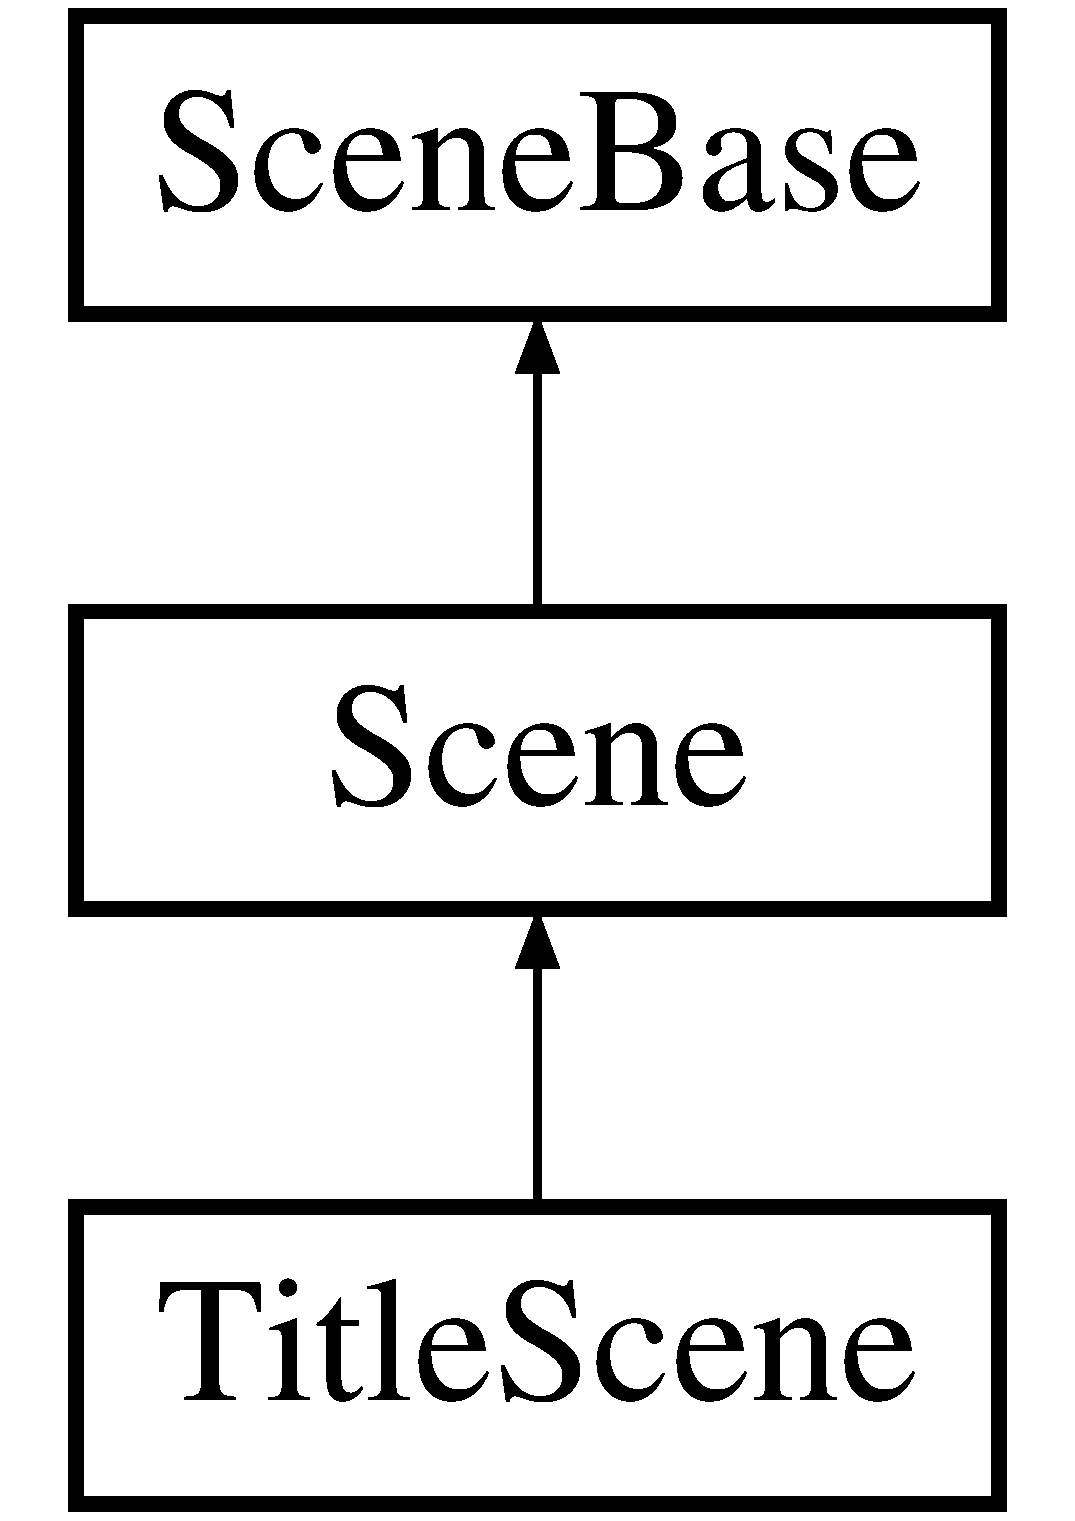
\includegraphics[height=3.000000cm]{class_title_scene}
\end{center}
\end{figure}
\subsection*{公開メンバ関数}
\begin{DoxyCompactItemize}
\item 
void \mbox{\hyperlink{class_title_scene_a3d039e7db0fa1e22e8c36d3cedfbd318}{Init}} () final
\begin{DoxyCompactList}\small\item\em タイトルシーンの初期化 \end{DoxyCompactList}\item 
\mbox{\hyperlink{scene__base_8h_a24cee5343fb9d0706ead6e8601f363be}{S\+C\+E\+NE}} \mbox{\hyperlink{class_title_scene_a19f6ee49ca6c8526fb1af2c0a2df9a33}{Update}} () final
\begin{DoxyCompactList}\small\item\em タイトルシーンの更新 \end{DoxyCompactList}\item 
void \mbox{\hyperlink{class_title_scene_af12c59b3bf9458640938c5ca620527ae}{Render}} () final
\begin{DoxyCompactList}\small\item\em タイトルシーンの描画 \end{DoxyCompactList}\item 
void \mbox{\hyperlink{class_title_scene_adfbc5f934572ede2e36419b089c88fe8}{Destroy}} () final
\begin{DoxyCompactList}\small\item\em タイトルシーンの破棄 \end{DoxyCompactList}\end{DoxyCompactItemize}
\subsection*{その他の継承メンバ}


\subsection{詳解}
タイトルシーンクラス 

\subsection{関数詳解}
\mbox{\Hypertarget{class_title_scene_adfbc5f934572ede2e36419b089c88fe8}\label{class_title_scene_adfbc5f934572ede2e36419b089c88fe8}} 
\index{Title\+Scene@{Title\+Scene}!Destroy@{Destroy}}
\index{Destroy@{Destroy}!Title\+Scene@{Title\+Scene}}
\subsubsection{\texorpdfstring{Destroy()}{Destroy()}}
{\footnotesize\ttfamily void Title\+Scene\+::\+Destroy (\begin{DoxyParamCaption}{ }\end{DoxyParamCaption})\hspace{0.3cm}{\ttfamily [final]}, {\ttfamily [virtual]}}



タイトルシーンの破棄 



\mbox{\hyperlink{class_scene_base_a7c5b54020bc519b4dadfe9770d6b27f7}{Scene\+Base}}を実装しています。

\mbox{\Hypertarget{class_title_scene_a3d039e7db0fa1e22e8c36d3cedfbd318}\label{class_title_scene_a3d039e7db0fa1e22e8c36d3cedfbd318}} 
\index{Title\+Scene@{Title\+Scene}!Init@{Init}}
\index{Init@{Init}!Title\+Scene@{Title\+Scene}}
\subsubsection{\texorpdfstring{Init()}{Init()}}
{\footnotesize\ttfamily void Title\+Scene\+::\+Init (\begin{DoxyParamCaption}{ }\end{DoxyParamCaption})\hspace{0.3cm}{\ttfamily [final]}, {\ttfamily [virtual]}}



タイトルシーンの初期化 



\mbox{\hyperlink{class_scene_base_a24d7db43c819924dc8b07b436f6d3148}{Scene\+Base}}を実装しています。

\mbox{\Hypertarget{class_title_scene_af12c59b3bf9458640938c5ca620527ae}\label{class_title_scene_af12c59b3bf9458640938c5ca620527ae}} 
\index{Title\+Scene@{Title\+Scene}!Render@{Render}}
\index{Render@{Render}!Title\+Scene@{Title\+Scene}}
\subsubsection{\texorpdfstring{Render()}{Render()}}
{\footnotesize\ttfamily void Title\+Scene\+::\+Render (\begin{DoxyParamCaption}{ }\end{DoxyParamCaption})\hspace{0.3cm}{\ttfamily [final]}, {\ttfamily [virtual]}}



タイトルシーンの描画 



\mbox{\hyperlink{class_scene_base_ad981674ce731ea267f398e889bbb9dc3}{Scene\+Base}}を実装しています。

\mbox{\Hypertarget{class_title_scene_a19f6ee49ca6c8526fb1af2c0a2df9a33}\label{class_title_scene_a19f6ee49ca6c8526fb1af2c0a2df9a33}} 
\index{Title\+Scene@{Title\+Scene}!Update@{Update}}
\index{Update@{Update}!Title\+Scene@{Title\+Scene}}
\subsubsection{\texorpdfstring{Update()}{Update()}}
{\footnotesize\ttfamily \mbox{\hyperlink{scene__base_8h_a24cee5343fb9d0706ead6e8601f363be}{S\+C\+E\+NE}} Title\+Scene\+::\+Update (\begin{DoxyParamCaption}{ }\end{DoxyParamCaption})\hspace{0.3cm}{\ttfamily [final]}, {\ttfamily [virtual]}}



タイトルシーンの更新 

\begin{DoxyReturn}{戻り値}
S\+C\+E\+NE シーンが変わるなら次のシーンのenum classを返す 
\end{DoxyReturn}


\mbox{\hyperlink{class_scene_acb50f8104e5a7cfecbdececa7d5f1b39}{Scene}}を実装しています。



このクラス詳解は次のファイルから抽出されました\+:\begin{DoxyCompactItemize}
\item 
C\+:/\+Users/tokir/\+Documents/\+Git\+Hub/\+Weapon\+Merchant\+Adventure/src/scene/main/title/\mbox{\hyperlink{title__scene_8h}{title\+\_\+scene.\+h}}\item 
C\+:/\+Users/tokir/\+Documents/\+Git\+Hub/\+Weapon\+Merchant\+Adventure/src/scene/main/title/\mbox{\hyperlink{title__scene_8cpp}{title\+\_\+scene.\+cpp}}\end{DoxyCompactItemize}

\hypertarget{class_transform}{}\section{Transform クラス}
\label{class_transform}\index{Transform@{Transform}}


{\ttfamily \#include $<$transform.\+h$>$}

\subsection*{公開メンバ関数}
\begin{DoxyCompactItemize}
\item 
\mbox{\hyperlink{class_transform_aa08ca4266efabc768973cdeea51945ab}{Transform}} ()
\item 
\mbox{\hyperlink{class_transform_afdda2868df3ca6b122c5e52f7919a692}{Transform}} (const float, const float=0, const float=0, const float=1)
\begin{DoxyCompactList}\small\item\em posをそれぞれのパラメータで受け取るコンストラクタ \end{DoxyCompactList}\item 
\mbox{\hyperlink{class_transform_aae9fd575f9e6e4862ea2d9232340e6dd}{Transform}} (const \mbox{\hyperlink{transform_8h_afb0c5e21d4133ff4f200992c0b534e1b}{V\+E\+C2}} \&\+\_\+pos, const float \+\_\+rot, const float \+\_\+scale)
\begin{DoxyCompactList}\small\item\em posを\+V\+E\+C2クラスで受け取るコンストラクタ \end{DoxyCompactList}\item 
\mbox{\hyperlink{class_transform_a7790f3c5dfe2b7fe7997af5f23e2ec7d}{Transform}} (const \mbox{\hyperlink{class_transform}{Transform}} \&t)
\begin{DoxyCompactList}\small\item\em コピーコンストラクタ \end{DoxyCompactList}\item 
void \mbox{\hyperlink{class_transform_a39816379bc1e3a0bbae23fa94db576f1}{Init}} (const float, const float=0, const float=0, const float=1)
\begin{DoxyCompactList}\small\item\em 一つ一つ値で渡す初期化 \end{DoxyCompactList}\item 
void \mbox{\hyperlink{class_transform_a0ccfc45e47071b7ebed1a61a14a202c4}{Init}} (const \mbox{\hyperlink{transform_8h_afb0c5e21d4133ff4f200992c0b534e1b}{V\+E\+C2}} \&\+\_\+pos, const float \+\_\+rot, const float \+\_\+scale)
\begin{DoxyCompactList}\small\item\em 各クラスに対して値を渡す初期化 \end{DoxyCompactList}\item 
void \mbox{\hyperlink{class_transform_a2d0cb73aca3f73de81f2bf8463cdb942}{Init}} (const \mbox{\hyperlink{class_transform}{Transform}} \&t)
\begin{DoxyCompactList}\small\item\em Transformクラスを渡す初期化 \end{DoxyCompactList}\item 
void \mbox{\hyperlink{class_transform_a45772ecb47b60d5b3f110613c3f15984}{Move}} (const float, const float)
\begin{DoxyCompactList}\small\item\em 一つ一つ値で渡す移動 \end{DoxyCompactList}\item 
void \mbox{\hyperlink{class_transform_a13dbb800ca989856d1f56c03dd9a0ad0}{Move}} (const \mbox{\hyperlink{transform_8h_afb0c5e21d4133ff4f200992c0b534e1b}{V\+E\+C2}} \&)
\begin{DoxyCompactList}\small\item\em  クラスで渡す移動 \end{DoxyCompactList}\item 
void \mbox{\hyperlink{class_transform_a696d7e837eafa09409150fb055daa223}{Rotate}} (const float)
\begin{DoxyCompactList}\small\item\em  回転 \end{DoxyCompactList}\item 
void \mbox{\hyperlink{class_transform_ad6097ddf1d30f5a1023725efbee375fb}{Scaling}} (const float)
\begin{DoxyCompactList}\small\item\em  拡大・縮小 \end{DoxyCompactList}\item 
void \mbox{\hyperlink{class_transform_af1a25489903986022218a798e4f40251}{operator=}} (const \mbox{\hyperlink{class_transform}{Transform}} \&)
\item 
void \mbox{\hyperlink{class_transform_a3b0aa54a1ca373ec3a7052977b5bf826}{operator+=}} (const \mbox{\hyperlink{class_transform}{Transform}} \&)
\item 
void \mbox{\hyperlink{class_transform_a204ee3471c1d08188076e3645c9f3517}{operator-\/=}} (const \mbox{\hyperlink{class_transform}{Transform}} \&)
\item 
void \mbox{\hyperlink{class_transform_a3746d6759ca289e8cd4982e889e7ec6b}{operator$\ast$=}} (const \mbox{\hyperlink{class_transform}{Transform}} \&)
\item 
void \mbox{\hyperlink{class_transform_ab13378f63abf5bc132841f83423a634d}{operator$\ast$=}} (const float)
\item 
void \mbox{\hyperlink{class_transform_aa38455bbe5aed5f9dfd98a8d3b8a24ec}{operator/=}} (const float)
\item 
\mbox{\hyperlink{class_transform}{Transform}} \mbox{\hyperlink{class_transform_a8e21c258146adde8ca798878bab9ce9d}{operator+}} (const \mbox{\hyperlink{class_transform}{Transform}} \&) const
\item 
\mbox{\hyperlink{class_transform}{Transform}} \mbox{\hyperlink{class_transform_a17493155309aa1650de99ce384f096a6}{operator-\/}} (const \mbox{\hyperlink{class_transform}{Transform}} \&) const
\item 
bool \mbox{\hyperlink{class_transform_a0a2d49f8c1b9a2229846534f9bcc63d4}{operator==}} (const \mbox{\hyperlink{class_transform}{Transform}} \&) const
\item 
bool \mbox{\hyperlink{class_transform_ae0aed78dcd6aaeb786ec0bdadafa9498}{operator!=}} (const \mbox{\hyperlink{class_transform}{Transform}} \&) const
\end{DoxyCompactItemize}
\subsection*{公開変数類}
\begin{DoxyCompactItemize}
\item 
\mbox{\hyperlink{transform_8h_afb0c5e21d4133ff4f200992c0b534e1b}{V\+E\+C2}} \mbox{\hyperlink{class_transform_a25bce2389cc280e8adf193bdbb00d94a}{pos}}
\item 
float \mbox{\hyperlink{class_transform_a2b471ae0000c6959dc9b07263933aa43}{rot}}
\item 
float \mbox{\hyperlink{class_transform_a631712eb230305f58d164086d492701b}{scale}}
\item 
\mbox{\hyperlink{transform_8h_afb0c5e21d4133ff4f200992c0b534e1b}{V\+E\+C2}} \mbox{\hyperlink{class_transform_a83e0bdbf8a2b4a45197d17d7415a6874}{size}}
\end{DoxyCompactItemize}


\subsection{詳解}
クラス 

\subsection{構築子と解体子}
\mbox{\Hypertarget{class_transform_aa08ca4266efabc768973cdeea51945ab}\label{class_transform_aa08ca4266efabc768973cdeea51945ab}} 
\index{Transform@{Transform}!Transform@{Transform}}
\index{Transform@{Transform}!Transform@{Transform}}
\subsubsection{\texorpdfstring{Transform()}{Transform()}\hspace{0.1cm}{\footnotesize\ttfamily [1/4]}}
{\footnotesize\ttfamily Transform\+::\+Transform (\begin{DoxyParamCaption}{ }\end{DoxyParamCaption})}

\+:brief ゼロで初期化する引数なしコンストラクタ \mbox{\Hypertarget{class_transform_afdda2868df3ca6b122c5e52f7919a692}\label{class_transform_afdda2868df3ca6b122c5e52f7919a692}} 
\index{Transform@{Transform}!Transform@{Transform}}
\index{Transform@{Transform}!Transform@{Transform}}
\subsubsection{\texorpdfstring{Transform()}{Transform()}\hspace{0.1cm}{\footnotesize\ttfamily [2/4]}}
{\footnotesize\ttfamily Transform\+::\+Transform (\begin{DoxyParamCaption}\item[{const float}]{posx,  }\item[{const float}]{posy = {\ttfamily 0},  }\item[{const float}]{\+\_\+rot = {\ttfamily 0},  }\item[{const float}]{\+\_\+scale = {\ttfamily 1} }\end{DoxyParamCaption})}



posをそれぞれのパラメータで受け取るコンストラクタ 

\mbox{\Hypertarget{class_transform_aae9fd575f9e6e4862ea2d9232340e6dd}\label{class_transform_aae9fd575f9e6e4862ea2d9232340e6dd}} 
\index{Transform@{Transform}!Transform@{Transform}}
\index{Transform@{Transform}!Transform@{Transform}}
\subsubsection{\texorpdfstring{Transform()}{Transform()}\hspace{0.1cm}{\footnotesize\ttfamily [3/4]}}
{\footnotesize\ttfamily Transform\+::\+Transform (\begin{DoxyParamCaption}\item[{const \mbox{\hyperlink{transform_8h_afb0c5e21d4133ff4f200992c0b534e1b}{V\+E\+C2}} \&}]{\+\_\+pos,  }\item[{const float}]{\+\_\+rot,  }\item[{const float}]{\+\_\+scale }\end{DoxyParamCaption})}



posを\+V\+E\+C2クラスで受け取るコンストラクタ 

\mbox{\Hypertarget{class_transform_a7790f3c5dfe2b7fe7997af5f23e2ec7d}\label{class_transform_a7790f3c5dfe2b7fe7997af5f23e2ec7d}} 
\index{Transform@{Transform}!Transform@{Transform}}
\index{Transform@{Transform}!Transform@{Transform}}
\subsubsection{\texorpdfstring{Transform()}{Transform()}\hspace{0.1cm}{\footnotesize\ttfamily [4/4]}}
{\footnotesize\ttfamily Transform\+::\+Transform (\begin{DoxyParamCaption}\item[{const \mbox{\hyperlink{class_transform}{Transform}} \&}]{t }\end{DoxyParamCaption})}



コピーコンストラクタ 



\subsection{関数詳解}
\mbox{\Hypertarget{class_transform_a39816379bc1e3a0bbae23fa94db576f1}\label{class_transform_a39816379bc1e3a0bbae23fa94db576f1}} 
\index{Transform@{Transform}!Init@{Init}}
\index{Init@{Init}!Transform@{Transform}}
\subsubsection{\texorpdfstring{Init()}{Init()}\hspace{0.1cm}{\footnotesize\ttfamily [1/3]}}
{\footnotesize\ttfamily void Transform\+::\+Init (\begin{DoxyParamCaption}\item[{const float}]{posx,  }\item[{const float}]{posy = {\ttfamily 0},  }\item[{const float}]{\+\_\+rot = {\ttfamily 0},  }\item[{const float}]{\+\_\+scale = {\ttfamily 1} }\end{DoxyParamCaption})}



一つ一つ値で渡す初期化 

\mbox{\Hypertarget{class_transform_a0ccfc45e47071b7ebed1a61a14a202c4}\label{class_transform_a0ccfc45e47071b7ebed1a61a14a202c4}} 
\index{Transform@{Transform}!Init@{Init}}
\index{Init@{Init}!Transform@{Transform}}
\subsubsection{\texorpdfstring{Init()}{Init()}\hspace{0.1cm}{\footnotesize\ttfamily [2/3]}}
{\footnotesize\ttfamily void Transform\+::\+Init (\begin{DoxyParamCaption}\item[{const \mbox{\hyperlink{transform_8h_afb0c5e21d4133ff4f200992c0b534e1b}{V\+E\+C2}} \&}]{\+\_\+pos,  }\item[{const float}]{\+\_\+rot,  }\item[{const float}]{\+\_\+scale }\end{DoxyParamCaption})}



各クラスに対して値を渡す初期化 

\mbox{\Hypertarget{class_transform_a2d0cb73aca3f73de81f2bf8463cdb942}\label{class_transform_a2d0cb73aca3f73de81f2bf8463cdb942}} 
\index{Transform@{Transform}!Init@{Init}}
\index{Init@{Init}!Transform@{Transform}}
\subsubsection{\texorpdfstring{Init()}{Init()}\hspace{0.1cm}{\footnotesize\ttfamily [3/3]}}
{\footnotesize\ttfamily void Transform\+::\+Init (\begin{DoxyParamCaption}\item[{const \mbox{\hyperlink{class_transform}{Transform}} \&}]{t }\end{DoxyParamCaption})}



Transformクラスを渡す初期化 

\mbox{\Hypertarget{class_transform_a45772ecb47b60d5b3f110613c3f15984}\label{class_transform_a45772ecb47b60d5b3f110613c3f15984}} 
\index{Transform@{Transform}!Move@{Move}}
\index{Move@{Move}!Transform@{Transform}}
\subsubsection{\texorpdfstring{Move()}{Move()}\hspace{0.1cm}{\footnotesize\ttfamily [1/2]}}
{\footnotesize\ttfamily void Transform\+::\+Move (\begin{DoxyParamCaption}\item[{const float}]{x,  }\item[{const float}]{y }\end{DoxyParamCaption})}



一つ一つ値で渡す移動 

\mbox{\Hypertarget{class_transform_a13dbb800ca989856d1f56c03dd9a0ad0}\label{class_transform_a13dbb800ca989856d1f56c03dd9a0ad0}} 
\index{Transform@{Transform}!Move@{Move}}
\index{Move@{Move}!Transform@{Transform}}
\subsubsection{\texorpdfstring{Move()}{Move()}\hspace{0.1cm}{\footnotesize\ttfamily [2/2]}}
{\footnotesize\ttfamily void Transform\+::\+Move (\begin{DoxyParamCaption}\item[{const \mbox{\hyperlink{transform_8h_afb0c5e21d4133ff4f200992c0b534e1b}{V\+E\+C2}} \&}]{\+\_\+pos }\end{DoxyParamCaption})}



 クラスで渡す移動 

\mbox{\Hypertarget{class_transform_ae0aed78dcd6aaeb786ec0bdadafa9498}\label{class_transform_ae0aed78dcd6aaeb786ec0bdadafa9498}} 
\index{Transform@{Transform}!operator"!=@{operator"!=}}
\index{operator"!=@{operator"!=}!Transform@{Transform}}
\subsubsection{\texorpdfstring{operator"!=()}{operator!=()}}
{\footnotesize\ttfamily bool Transform\+::operator!= (\begin{DoxyParamCaption}\item[{const \mbox{\hyperlink{class_transform}{Transform}} \&}]{t }\end{DoxyParamCaption}) const}

\mbox{\Hypertarget{class_transform_a3746d6759ca289e8cd4982e889e7ec6b}\label{class_transform_a3746d6759ca289e8cd4982e889e7ec6b}} 
\index{Transform@{Transform}!operator$\ast$=@{operator$\ast$=}}
\index{operator$\ast$=@{operator$\ast$=}!Transform@{Transform}}
\subsubsection{\texorpdfstring{operator$\ast$=()}{operator*=()}\hspace{0.1cm}{\footnotesize\ttfamily [1/2]}}
{\footnotesize\ttfamily void Transform\+::operator$\ast$= (\begin{DoxyParamCaption}\item[{const \mbox{\hyperlink{class_transform}{Transform}} \&}]{t }\end{DoxyParamCaption})}

\mbox{\Hypertarget{class_transform_ab13378f63abf5bc132841f83423a634d}\label{class_transform_ab13378f63abf5bc132841f83423a634d}} 
\index{Transform@{Transform}!operator$\ast$=@{operator$\ast$=}}
\index{operator$\ast$=@{operator$\ast$=}!Transform@{Transform}}
\subsubsection{\texorpdfstring{operator$\ast$=()}{operator*=()}\hspace{0.1cm}{\footnotesize\ttfamily [2/2]}}
{\footnotesize\ttfamily void Transform\+::operator$\ast$= (\begin{DoxyParamCaption}\item[{const float}]{s }\end{DoxyParamCaption})}

\mbox{\Hypertarget{class_transform_a8e21c258146adde8ca798878bab9ce9d}\label{class_transform_a8e21c258146adde8ca798878bab9ce9d}} 
\index{Transform@{Transform}!operator+@{operator+}}
\index{operator+@{operator+}!Transform@{Transform}}
\subsubsection{\texorpdfstring{operator+()}{operator+()}}
{\footnotesize\ttfamily \mbox{\hyperlink{class_transform}{Transform}} Transform\+::operator+ (\begin{DoxyParamCaption}\item[{const \mbox{\hyperlink{class_transform}{Transform}} \&}]{t }\end{DoxyParamCaption}) const}

\mbox{\Hypertarget{class_transform_a3b0aa54a1ca373ec3a7052977b5bf826}\label{class_transform_a3b0aa54a1ca373ec3a7052977b5bf826}} 
\index{Transform@{Transform}!operator+=@{operator+=}}
\index{operator+=@{operator+=}!Transform@{Transform}}
\subsubsection{\texorpdfstring{operator+=()}{operator+=()}}
{\footnotesize\ttfamily void Transform\+::operator+= (\begin{DoxyParamCaption}\item[{const \mbox{\hyperlink{class_transform}{Transform}} \&}]{t }\end{DoxyParamCaption})}

\mbox{\Hypertarget{class_transform_a17493155309aa1650de99ce384f096a6}\label{class_transform_a17493155309aa1650de99ce384f096a6}} 
\index{Transform@{Transform}!operator-\/@{operator-\/}}
\index{operator-\/@{operator-\/}!Transform@{Transform}}
\subsubsection{\texorpdfstring{operator-\/()}{operator-()}}
{\footnotesize\ttfamily \mbox{\hyperlink{class_transform}{Transform}} Transform\+::operator-\/ (\begin{DoxyParamCaption}\item[{const \mbox{\hyperlink{class_transform}{Transform}} \&}]{t }\end{DoxyParamCaption}) const}

\mbox{\Hypertarget{class_transform_a204ee3471c1d08188076e3645c9f3517}\label{class_transform_a204ee3471c1d08188076e3645c9f3517}} 
\index{Transform@{Transform}!operator-\/=@{operator-\/=}}
\index{operator-\/=@{operator-\/=}!Transform@{Transform}}
\subsubsection{\texorpdfstring{operator-\/=()}{operator-=()}}
{\footnotesize\ttfamily void Transform\+::operator-\/= (\begin{DoxyParamCaption}\item[{const \mbox{\hyperlink{class_transform}{Transform}} \&}]{t }\end{DoxyParamCaption})}

\mbox{\Hypertarget{class_transform_aa38455bbe5aed5f9dfd98a8d3b8a24ec}\label{class_transform_aa38455bbe5aed5f9dfd98a8d3b8a24ec}} 
\index{Transform@{Transform}!operator/=@{operator/=}}
\index{operator/=@{operator/=}!Transform@{Transform}}
\subsubsection{\texorpdfstring{operator/=()}{operator/=()}}
{\footnotesize\ttfamily void Transform\+::operator/= (\begin{DoxyParamCaption}\item[{const float}]{s }\end{DoxyParamCaption})}

\mbox{\Hypertarget{class_transform_af1a25489903986022218a798e4f40251}\label{class_transform_af1a25489903986022218a798e4f40251}} 
\index{Transform@{Transform}!operator=@{operator=}}
\index{operator=@{operator=}!Transform@{Transform}}
\subsubsection{\texorpdfstring{operator=()}{operator=()}}
{\footnotesize\ttfamily void Transform\+::operator= (\begin{DoxyParamCaption}\item[{const \mbox{\hyperlink{class_transform}{Transform}} \&}]{t }\end{DoxyParamCaption})}

\mbox{\Hypertarget{class_transform_a0a2d49f8c1b9a2229846534f9bcc63d4}\label{class_transform_a0a2d49f8c1b9a2229846534f9bcc63d4}} 
\index{Transform@{Transform}!operator==@{operator==}}
\index{operator==@{operator==}!Transform@{Transform}}
\subsubsection{\texorpdfstring{operator==()}{operator==()}}
{\footnotesize\ttfamily bool Transform\+::operator== (\begin{DoxyParamCaption}\item[{const \mbox{\hyperlink{class_transform}{Transform}} \&}]{t }\end{DoxyParamCaption}) const}

\mbox{\Hypertarget{class_transform_a696d7e837eafa09409150fb055daa223}\label{class_transform_a696d7e837eafa09409150fb055daa223}} 
\index{Transform@{Transform}!Rotate@{Rotate}}
\index{Rotate@{Rotate}!Transform@{Transform}}
\subsubsection{\texorpdfstring{Rotate()}{Rotate()}}
{\footnotesize\ttfamily void Transform\+::\+Rotate (\begin{DoxyParamCaption}\item[{const float}]{\+\_\+rot }\end{DoxyParamCaption})}



 回転 

\mbox{\Hypertarget{class_transform_ad6097ddf1d30f5a1023725efbee375fb}\label{class_transform_ad6097ddf1d30f5a1023725efbee375fb}} 
\index{Transform@{Transform}!Scaling@{Scaling}}
\index{Scaling@{Scaling}!Transform@{Transform}}
\subsubsection{\texorpdfstring{Scaling()}{Scaling()}}
{\footnotesize\ttfamily void Transform\+::\+Scaling (\begin{DoxyParamCaption}\item[{const float}]{\+\_\+scale }\end{DoxyParamCaption})}



 拡大・縮小 



\subsection{メンバ詳解}
\mbox{\Hypertarget{class_transform_a25bce2389cc280e8adf193bdbb00d94a}\label{class_transform_a25bce2389cc280e8adf193bdbb00d94a}} 
\index{Transform@{Transform}!pos@{pos}}
\index{pos@{pos}!Transform@{Transform}}
\subsubsection{\texorpdfstring{pos}{pos}}
{\footnotesize\ttfamily \mbox{\hyperlink{transform_8h_afb0c5e21d4133ff4f200992c0b534e1b}{V\+E\+C2}} Transform\+::pos}

\mbox{\Hypertarget{class_transform_a2b471ae0000c6959dc9b07263933aa43}\label{class_transform_a2b471ae0000c6959dc9b07263933aa43}} 
\index{Transform@{Transform}!rot@{rot}}
\index{rot@{rot}!Transform@{Transform}}
\subsubsection{\texorpdfstring{rot}{rot}}
{\footnotesize\ttfamily float Transform\+::rot}

\mbox{\Hypertarget{class_transform_a631712eb230305f58d164086d492701b}\label{class_transform_a631712eb230305f58d164086d492701b}} 
\index{Transform@{Transform}!scale@{scale}}
\index{scale@{scale}!Transform@{Transform}}
\subsubsection{\texorpdfstring{scale}{scale}}
{\footnotesize\ttfamily float Transform\+::scale}

\mbox{\Hypertarget{class_transform_a83e0bdbf8a2b4a45197d17d7415a6874}\label{class_transform_a83e0bdbf8a2b4a45197d17d7415a6874}} 
\index{Transform@{Transform}!size@{size}}
\index{size@{size}!Transform@{Transform}}
\subsubsection{\texorpdfstring{size}{size}}
{\footnotesize\ttfamily \mbox{\hyperlink{transform_8h_afb0c5e21d4133ff4f200992c0b534e1b}{V\+E\+C2}} Transform\+::size}



このクラス詳解は次のファイルから抽出されました\+:\begin{DoxyCompactItemize}
\item 
C\+:/\+Users/tokir/\+Documents/\+Git\+Hub/\+Weapon\+Merchant\+Adventure/src/transform/\mbox{\hyperlink{transform_8h}{transform.\+h}}\item 
C\+:/\+Users/tokir/\+Documents/\+Git\+Hub/\+Weapon\+Merchant\+Adventure/src/transform/\mbox{\hyperlink{transform_8cpp}{transform.\+cpp}}\end{DoxyCompactItemize}

\hypertarget{class_ui_base}{}\section{Ui\+Base クラス}
\label{class_ui_base}\index{Ui\+Base@{Ui\+Base}}


{\ttfamily \#include $<$ui\+\_\+base.\+h$>$}

Ui\+Base の継承関係図\begin{figure}[H]
\begin{center}
\leavevmode
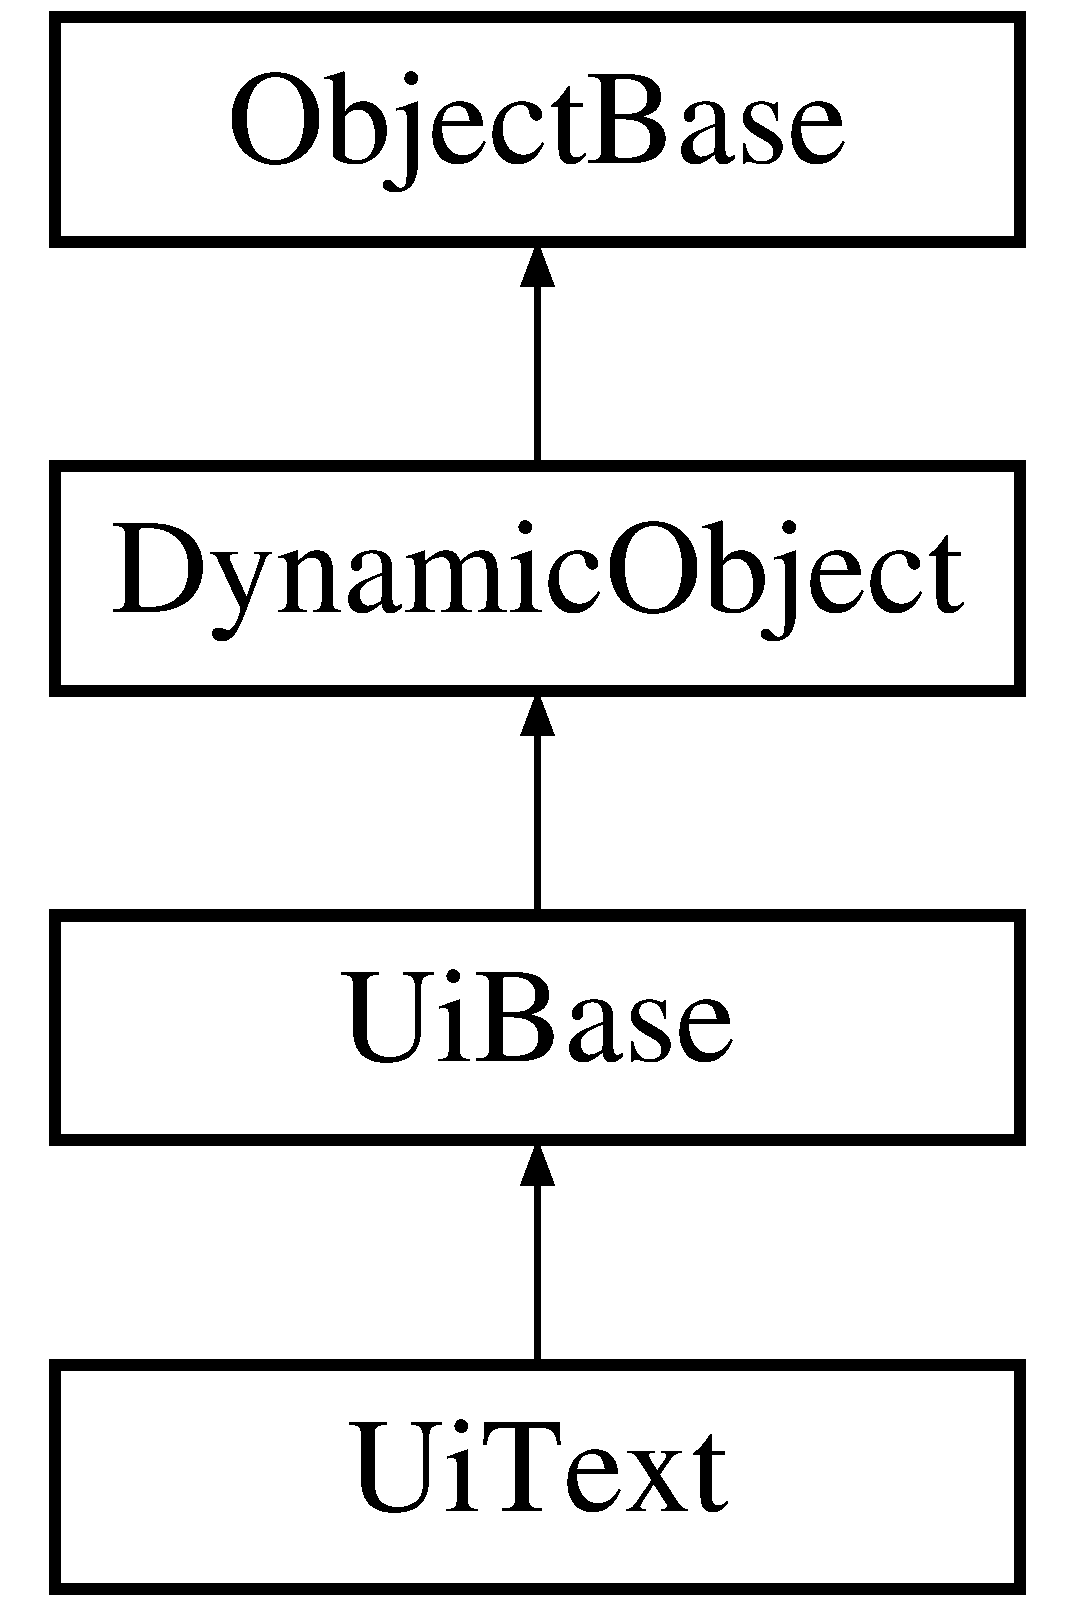
\includegraphics[height=4.000000cm]{class_ui_base}
\end{center}
\end{figure}
\subsection*{公開メンバ関数}
\begin{DoxyCompactItemize}
\item 
virtual \mbox{\hyperlink{class_ui_base_ac8713016ee88ba89e36897f3bbf72743}{$\sim$\+Ui\+Base}} ()
\end{DoxyCompactItemize}
\subsection*{その他の継承メンバ}


\subsection{構築子と解体子}
\mbox{\Hypertarget{class_ui_base_ac8713016ee88ba89e36897f3bbf72743}\label{class_ui_base_ac8713016ee88ba89e36897f3bbf72743}} 
\index{Ui\+Base@{Ui\+Base}!````~Ui\+Base@{$\sim$\+Ui\+Base}}
\index{````~Ui\+Base@{$\sim$\+Ui\+Base}!Ui\+Base@{Ui\+Base}}
\subsubsection{\texorpdfstring{$\sim$\+Ui\+Base()}{~UiBase()}}
{\footnotesize\ttfamily virtual Ui\+Base\+::$\sim$\+Ui\+Base (\begin{DoxyParamCaption}{ }\end{DoxyParamCaption})\hspace{0.3cm}{\ttfamily [inline]}, {\ttfamily [virtual]}}



このクラス詳解は次のファイルから抽出されました\+:\begin{DoxyCompactItemize}
\item 
C\+:/\+Users/tokir/\+Documents/\+Git\+Hub/\+Weapon\+Merchant\+Adventure/src/object/ui/base/\mbox{\hyperlink{ui__base_8h}{ui\+\_\+base.\+h}}\end{DoxyCompactItemize}

\hypertarget{class_ui_text}{}\section{Ui\+Text クラス}
\label{class_ui_text}\index{Ui\+Text@{Ui\+Text}}


テキストのuiクラス  




{\ttfamily \#include $<$ui\+\_\+text.\+h$>$}

Ui\+Text の継承関係図\begin{figure}[H]
\begin{center}
\leavevmode
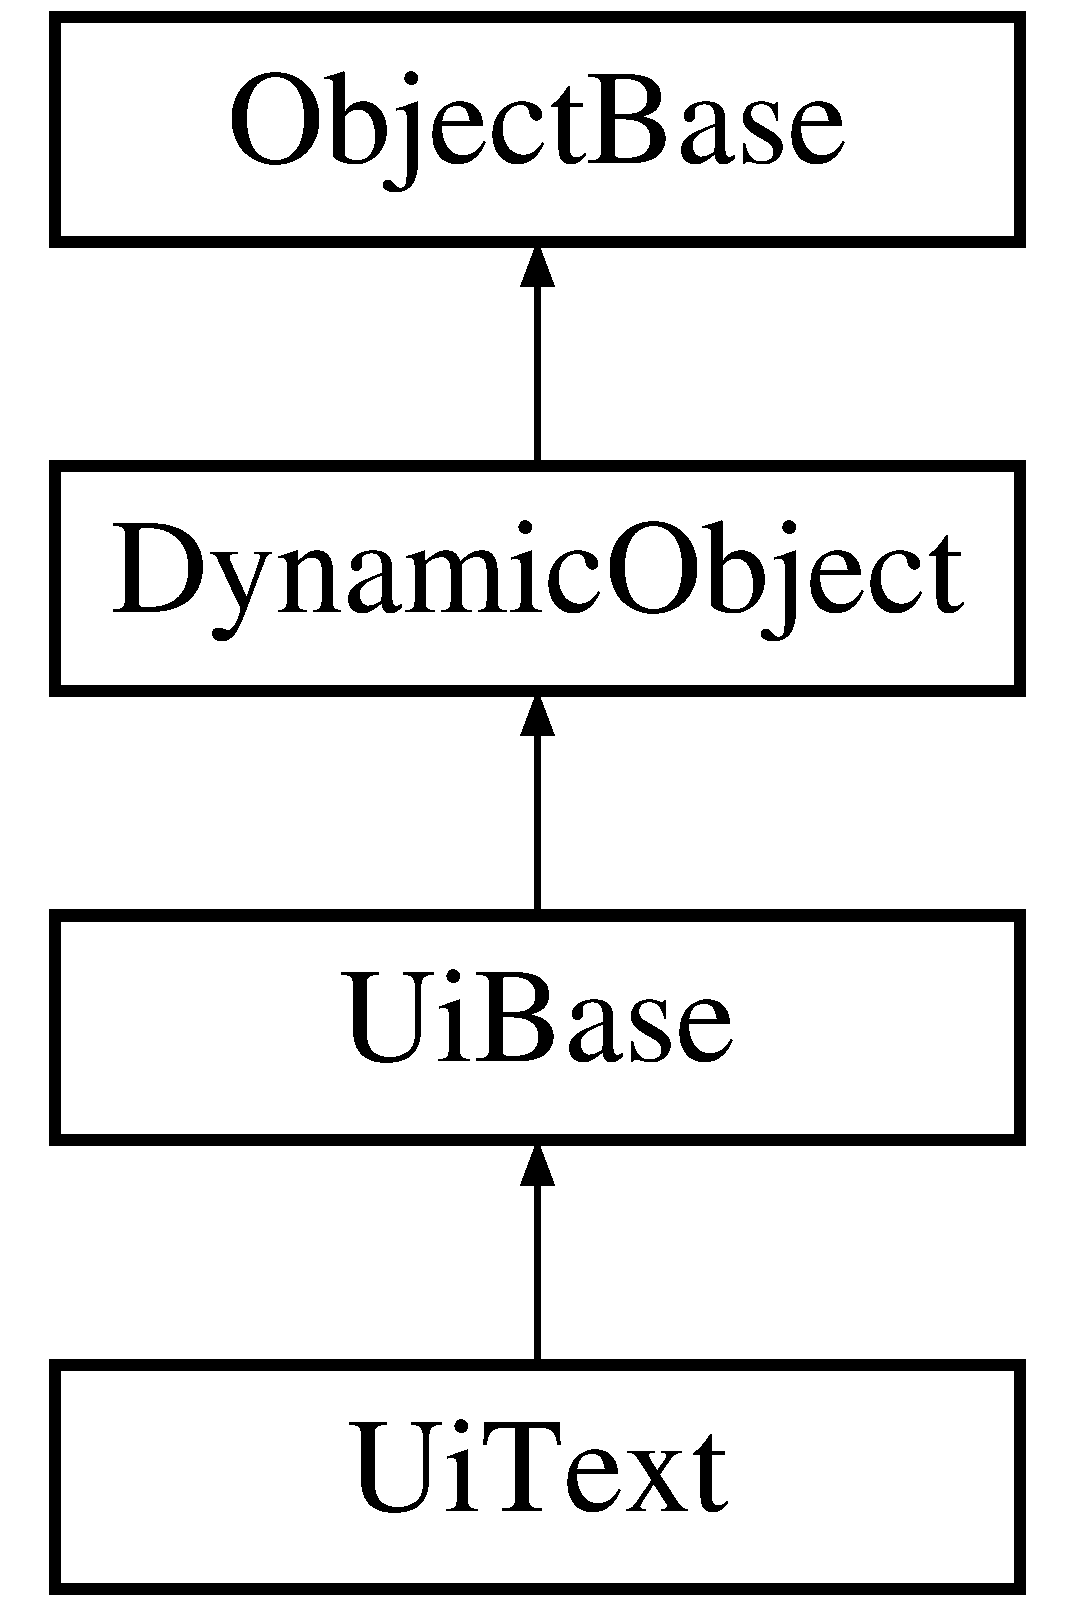
\includegraphics[height=4.000000cm]{class_ui_text}
\end{center}
\end{figure}
\subsection*{その他の継承メンバ}


\subsection{詳解}
テキストのuiクラス 

このクラス詳解は次のファイルから抽出されました\+:\begin{DoxyCompactItemize}
\item 
C\+:/\+Users/tokir/\+Documents/\+Git\+Hub/\+Weapon\+Merchant\+Adventure/src/object/ui/text/\mbox{\hyperlink{ui__text_8h}{ui\+\_\+text.\+h}}\end{DoxyCompactItemize}

\hypertarget{class_weapon_base}{}\section{Weapon\+Base クラス}
\label{class_weapon_base}\index{Weapon\+Base@{Weapon\+Base}}


武器のスーパークラス  




{\ttfamily \#include $<$weapon\+\_\+base.\+h$>$}

Weapon\+Base の継承関係図\begin{figure}[H]
\begin{center}
\leavevmode
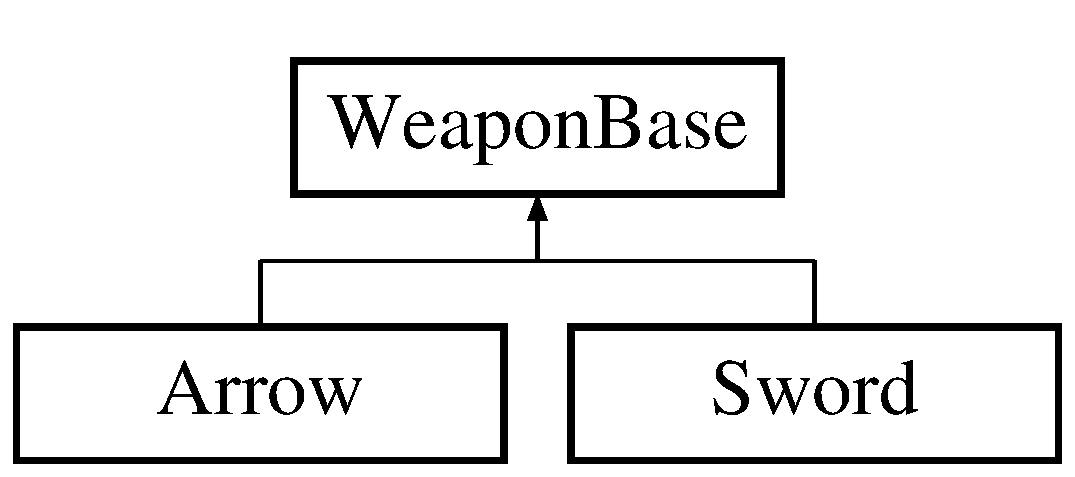
\includegraphics[height=2.000000cm]{class_weapon_base}
\end{center}
\end{figure}
\subsection*{公開メンバ関数}
\begin{DoxyCompactItemize}
\item 
virtual bool \mbox{\hyperlink{class_weapon_base_a1bab9c7fb9524db754bebbbcbf6c2fd9}{Attack}} (bool, const \mbox{\hyperlink{common_8h_ab1cb35b3a17c398d8ef71d5f779808bf}{Vec3}} \&)=0
\item 
virtual void \mbox{\hyperlink{class_weapon_base_a25cd4c351638b76377e93341a9545712}{Weapon\+Start}} ()=0
\item 
virtual void \mbox{\hyperlink{class_weapon_base_aa1e3d02353273ab72a71cc3a1563636a}{Weapon\+Update}} (const \mbox{\hyperlink{common_8h_ab1cb35b3a17c398d8ef71d5f779808bf}{Vec3}} \&, bool)=0
\item 
virtual void \mbox{\hyperlink{class_weapon_base_af308d16d3892c3ffaeedf74b08e761b9}{Weapon\+Render}} (const \mbox{\hyperlink{common_8h_a1c43cb8f0d8a41901f3ce4c67dbbce20}{Transform}} \&=\mbox{\hyperlink{common_8h_a1c43cb8f0d8a41901f3ce4c67dbbce20}{Transform}}\{ saki\+::vector3\+\_\+zero$<$ float $>$, saki\+::vector3\+\_\+zero$<$ float $>$, saki\+::vector3\+\_\+zero$<$ float $>$ \})=0
\item 
virtual void \mbox{\hyperlink{class_weapon_base_a417784a8c8bf73cd398a77b922fc110c}{Weapon\+Destroy}} ()=0
\item 
virtual \mbox{\hyperlink{class_weapon_base_a311bee6c8496581f21068867be48762f}{$\sim$\+Weapon\+Base}} ()
\end{DoxyCompactItemize}
\subsection*{公開変数類}
\begin{DoxyCompactItemize}
\item 
bool \mbox{\hyperlink{class_weapon_base_a54883e3ecbc54ff42ea381a17ef8cf8f}{weapon\+\_\+enabled}} = true
\end{DoxyCompactItemize}


\subsection{詳解}
武器のスーパークラス 

\subsection{構築子と解体子}
\mbox{\Hypertarget{class_weapon_base_a311bee6c8496581f21068867be48762f}\label{class_weapon_base_a311bee6c8496581f21068867be48762f}} 
\index{Weapon\+Base@{Weapon\+Base}!````~Weapon\+Base@{$\sim$\+Weapon\+Base}}
\index{````~Weapon\+Base@{$\sim$\+Weapon\+Base}!Weapon\+Base@{Weapon\+Base}}
\subsubsection{\texorpdfstring{$\sim$\+Weapon\+Base()}{~WeaponBase()}}
{\footnotesize\ttfamily virtual Weapon\+Base\+::$\sim$\+Weapon\+Base (\begin{DoxyParamCaption}{ }\end{DoxyParamCaption})\hspace{0.3cm}{\ttfamily [inline]}, {\ttfamily [virtual]}}



\subsection{関数詳解}
\mbox{\Hypertarget{class_weapon_base_a1bab9c7fb9524db754bebbbcbf6c2fd9}\label{class_weapon_base_a1bab9c7fb9524db754bebbbcbf6c2fd9}} 
\index{Weapon\+Base@{Weapon\+Base}!Attack@{Attack}}
\index{Attack@{Attack}!Weapon\+Base@{Weapon\+Base}}
\subsubsection{\texorpdfstring{Attack()}{Attack()}}
{\footnotesize\ttfamily virtual bool Weapon\+Base\+::\+Attack (\begin{DoxyParamCaption}\item[{bool}]{,  }\item[{const \mbox{\hyperlink{common_8h_ab1cb35b3a17c398d8ef71d5f779808bf}{Vec3}} \&}]{ }\end{DoxyParamCaption})\hspace{0.3cm}{\ttfamily [pure virtual]}}



\mbox{\hyperlink{class_sword_a6c8642e6a8f1d6152abce6c84bf6d21b}{Sword}}, \mbox{\hyperlink{class_arrow_a98ea469bf0b21635b2d2dadb69c72240}{Arrow}}で実装されています。

\mbox{\Hypertarget{class_weapon_base_a417784a8c8bf73cd398a77b922fc110c}\label{class_weapon_base_a417784a8c8bf73cd398a77b922fc110c}} 
\index{Weapon\+Base@{Weapon\+Base}!Weapon\+Destroy@{Weapon\+Destroy}}
\index{Weapon\+Destroy@{Weapon\+Destroy}!Weapon\+Base@{Weapon\+Base}}
\subsubsection{\texorpdfstring{Weapon\+Destroy()}{WeaponDestroy()}}
{\footnotesize\ttfamily virtual void Weapon\+Base\+::\+Weapon\+Destroy (\begin{DoxyParamCaption}{ }\end{DoxyParamCaption})\hspace{0.3cm}{\ttfamily [pure virtual]}}



\mbox{\hyperlink{class_sword_a3f60d8b24b7847d6a84f0941820b711d}{Sword}}, \mbox{\hyperlink{class_arrow_a1101d1159771b5c428afd3c7a6a0a4df}{Arrow}}で実装されています。

\mbox{\Hypertarget{class_weapon_base_af308d16d3892c3ffaeedf74b08e761b9}\label{class_weapon_base_af308d16d3892c3ffaeedf74b08e761b9}} 
\index{Weapon\+Base@{Weapon\+Base}!Weapon\+Render@{Weapon\+Render}}
\index{Weapon\+Render@{Weapon\+Render}!Weapon\+Base@{Weapon\+Base}}
\subsubsection{\texorpdfstring{Weapon\+Render()}{WeaponRender()}}
{\footnotesize\ttfamily virtual void Weapon\+Base\+::\+Weapon\+Render (\begin{DoxyParamCaption}\item[{const \mbox{\hyperlink{common_8h_a1c43cb8f0d8a41901f3ce4c67dbbce20}{Transform}} \&}]{ = {\ttfamily \mbox{\hyperlink{common_8h_a1c43cb8f0d8a41901f3ce4c67dbbce20}{Transform}}\{~saki\+:\+:vector3\+\_\+zero$<$~float~$>$,~saki\+:\+:vector3\+\_\+zero$<$~float~$>$,~saki\+:\+:vector3\+\_\+zero$<$~float~$>$~\}} }\end{DoxyParamCaption})\hspace{0.3cm}{\ttfamily [pure virtual]}}



\mbox{\hyperlink{class_sword_ac80e3b54ef5572eae1e4760d14383f4f}{Sword}}, \mbox{\hyperlink{class_arrow_af9e54760156a77a15ad98a88f712ebdb}{Arrow}}で実装されています。

\mbox{\Hypertarget{class_weapon_base_a25cd4c351638b76377e93341a9545712}\label{class_weapon_base_a25cd4c351638b76377e93341a9545712}} 
\index{Weapon\+Base@{Weapon\+Base}!Weapon\+Start@{Weapon\+Start}}
\index{Weapon\+Start@{Weapon\+Start}!Weapon\+Base@{Weapon\+Base}}
\subsubsection{\texorpdfstring{Weapon\+Start()}{WeaponStart()}}
{\footnotesize\ttfamily virtual void Weapon\+Base\+::\+Weapon\+Start (\begin{DoxyParamCaption}{ }\end{DoxyParamCaption})\hspace{0.3cm}{\ttfamily [pure virtual]}}



\mbox{\hyperlink{class_sword_af9027f627d1db6c0ac21d2aa842cff69}{Sword}}, \mbox{\hyperlink{class_arrow_a085b5bd5f9e3ce25a081b502f9989f33}{Arrow}}で実装されています。

\mbox{\Hypertarget{class_weapon_base_aa1e3d02353273ab72a71cc3a1563636a}\label{class_weapon_base_aa1e3d02353273ab72a71cc3a1563636a}} 
\index{Weapon\+Base@{Weapon\+Base}!Weapon\+Update@{Weapon\+Update}}
\index{Weapon\+Update@{Weapon\+Update}!Weapon\+Base@{Weapon\+Base}}
\subsubsection{\texorpdfstring{Weapon\+Update()}{WeaponUpdate()}}
{\footnotesize\ttfamily virtual void Weapon\+Base\+::\+Weapon\+Update (\begin{DoxyParamCaption}\item[{const \mbox{\hyperlink{common_8h_ab1cb35b3a17c398d8ef71d5f779808bf}{Vec3}} \&}]{,  }\item[{bool}]{ }\end{DoxyParamCaption})\hspace{0.3cm}{\ttfamily [pure virtual]}}



\mbox{\hyperlink{class_sword_a5fda2f72829b6256ffc3fb18d9d065e8}{Sword}}, \mbox{\hyperlink{class_arrow_afb6110035cba7b850d12755570163b29}{Arrow}}で実装されています。



\subsection{メンバ詳解}
\mbox{\Hypertarget{class_weapon_base_a54883e3ecbc54ff42ea381a17ef8cf8f}\label{class_weapon_base_a54883e3ecbc54ff42ea381a17ef8cf8f}} 
\index{Weapon\+Base@{Weapon\+Base}!weapon\+\_\+enabled@{weapon\+\_\+enabled}}
\index{weapon\+\_\+enabled@{weapon\+\_\+enabled}!Weapon\+Base@{Weapon\+Base}}
\subsubsection{\texorpdfstring{weapon\+\_\+enabled}{weapon\_enabled}}
{\footnotesize\ttfamily bool Weapon\+Base\+::weapon\+\_\+enabled = true}



このクラス詳解は次のファイルから抽出されました\+:\begin{DoxyCompactItemize}
\item 
C\+:/\+Users/tokir/\+Documents/\+Git\+Hub/\+Weapon\+Merchant\+Adventure/src/src/object/weapon/base/\mbox{\hyperlink{weapon__base_8h}{weapon\+\_\+base.\+h}}\end{DoxyCompactItemize}

\chapter{ファイル詳解}
\hypertarget{animation_8cpp}{}\section{C\+:/\+Users/tokir/\+Documents/\+Git\+Hub/\+Weapon\+Merchant\+Adventure/src/animation/animation.cpp ファイル}
\label{animation_8cpp}\index{C\+:/\+Users/tokir/\+Documents/\+Git\+Hub/\+Weapon\+Merchant\+Adventure/src/animation/animation.\+cpp@{C\+:/\+Users/tokir/\+Documents/\+Git\+Hub/\+Weapon\+Merchant\+Adventure/src/animation/animation.\+cpp}}


アニメーションクラスのメンバ関数を定義  


{\ttfamily \#include \char`\"{}animation.\+h\char`\"{}}\newline


\subsection{詳解}
アニメーションクラスのメンバ関数を定義 

\begin{DoxyAuthor}{著者}
石山 悠 
\end{DoxyAuthor}
\begin{DoxyDate}{日付}
2018/10/29 
\end{DoxyDate}

\hypertarget{animation_8h}{}\section{C\+:/\+Users/tokir/\+Documents/\+Git\+Hub/\+Weapon\+Merchant\+Adventure/src/animation/animation.h ファイル}
\label{animation_8h}\index{C\+:/\+Users/tokir/\+Documents/\+Git\+Hub/\+Weapon\+Merchant\+Adventure/src/animation/animation.\+h@{C\+:/\+Users/tokir/\+Documents/\+Git\+Hub/\+Weapon\+Merchant\+Adventure/src/animation/animation.\+h}}


アニメーションクラスの宣言  


{\ttfamily \#include \char`\"{}../transform/transform.\+h\char`\"{}}\newline
\subsection*{クラス}
\begin{DoxyCompactItemize}
\item 
class \mbox{\hyperlink{class_animation}{Animation}}
\begin{DoxyCompactList}\small\item\em アニメーションクラス \end{DoxyCompactList}\end{DoxyCompactItemize}


\subsection{詳解}
アニメーションクラスの宣言 

\begin{DoxyAuthor}{著者}
石山 悠 
\end{DoxyAuthor}
\begin{DoxyDate}{日付}
2018/10/29 
\end{DoxyDate}

\hypertarget{collider__base_8h}{}\section{C\+:/\+Users/tokir/\+Documents/\+Git\+Hub/\+Weapon\+Merchant\+Adventure/src/src/collider/base/collider\+\_\+base.h ファイル}
\label{collider__base_8h}\index{C\+:/\+Users/tokir/\+Documents/\+Git\+Hub/\+Weapon\+Merchant\+Adventure/src/src/collider/base/collider\+\_\+base.\+h@{C\+:/\+Users/tokir/\+Documents/\+Git\+Hub/\+Weapon\+Merchant\+Adventure/src/src/collider/base/collider\+\_\+base.\+h}}


コライダのスーパークラスの宣言、定義  


{\ttfamily \#include \char`\"{}../../common/common.\+h\char`\"{}}\newline
{\ttfamily \#include \char`\"{}../../object/base/object\+\_\+base.\+h\char`\"{}}\newline
{\ttfamily \#include $<$functional$>$}\newline
\subsection*{クラス}
\begin{DoxyCompactItemize}
\item 
class \mbox{\hyperlink{class_collider_base}{Collider\+Base}}
\begin{DoxyCompactList}\small\item\em コライダのスーパークラス \end{DoxyCompactList}\end{DoxyCompactItemize}


\subsection{詳解}
コライダのスーパークラスの宣言、定義 

\begin{DoxyAuthor}{著者}
石山 悠 
\end{DoxyAuthor}
\begin{DoxyDate}{日付}
2018/10/11 
\end{DoxyDate}

\hypertarget{collider__manager_8cpp}{}\section{C\+:/\+Users/tokir/\+Documents/\+Git\+Hub/\+Weapon\+Merchant\+Adventure/src/collider/manager/collider\+\_\+manager.cpp ファイル}
\label{collider__manager_8cpp}\index{C\+:/\+Users/tokir/\+Documents/\+Git\+Hub/\+Weapon\+Merchant\+Adventure/src/collider/manager/collider\+\_\+manager.\+cpp@{C\+:/\+Users/tokir/\+Documents/\+Git\+Hub/\+Weapon\+Merchant\+Adventure/src/collider/manager/collider\+\_\+manager.\+cpp}}


コライダを管理するクラスのメンバ関数を定義  


{\ttfamily \#include \char`\"{}collider\+\_\+manager.\+h\char`\"{}}\newline


\subsection{詳解}
コライダを管理するクラスのメンバ関数を定義 

\begin{DoxyAuthor}{著者}
石山 悠 
\end{DoxyAuthor}
\begin{DoxyDate}{日付}
2018/10/11 
\end{DoxyDate}

\hypertarget{collider__manager_8h}{}\section{C\+:/\+Users/tokir/\+Documents/\+Git\+Hub/\+Weapon\+Merchant\+Adventure/src/collider/manager/collider\+\_\+manager.h ファイル}
\label{collider__manager_8h}\index{C\+:/\+Users/tokir/\+Documents/\+Git\+Hub/\+Weapon\+Merchant\+Adventure/src/collider/manager/collider\+\_\+manager.\+h@{C\+:/\+Users/tokir/\+Documents/\+Git\+Hub/\+Weapon\+Merchant\+Adventure/src/collider/manager/collider\+\_\+manager.\+h}}


コライダを管理するクラスを宣言  


{\ttfamily \#include \char`\"{}../../common/singleton.\+h\char`\"{}}\newline
{\ttfamily \#include \char`\"{}../square/square\+\_\+collider.\+h\char`\"{}}\newline
{\ttfamily \#include $<$vector$>$}\newline
\subsection*{クラス}
\begin{DoxyCompactItemize}
\item 
class \mbox{\hyperlink{class_collider_manager}{Collider\+Manager}}
\begin{DoxyCompactList}\small\item\em コライダを管理するクラス \end{DoxyCompactList}\end{DoxyCompactItemize}


\subsection{詳解}
コライダを管理するクラスを宣言 

\begin{DoxyAuthor}{著者}
石山 悠 
\end{DoxyAuthor}
\begin{DoxyDate}{日付}
2018/10/09 
\end{DoxyDate}

\hypertarget{square__collider_8cpp}{}\section{C\+:/\+Users/tokir/\+Documents/\+Git\+Hub/\+Weapon\+Merchant\+Adventure/src/collider/square/square\+\_\+collider.cpp ファイル}
\label{square__collider_8cpp}\index{C\+:/\+Users/tokir/\+Documents/\+Git\+Hub/\+Weapon\+Merchant\+Adventure/src/collider/square/square\+\_\+collider.\+cpp@{C\+:/\+Users/tokir/\+Documents/\+Git\+Hub/\+Weapon\+Merchant\+Adventure/src/collider/square/square\+\_\+collider.\+cpp}}


四角形のコライダクラスのメンバ関数を定義  


{\ttfamily \#include \char`\"{}square\+\_\+collider.\+h\char`\"{}}\newline
{\ttfamily \#include \char`\"{}../manager/collider\+\_\+manager.\+h\char`\"{}}\newline


\subsection{詳解}
四角形のコライダクラスのメンバ関数を定義 

\begin{DoxyAuthor}{著者}
石山 悠 
\end{DoxyAuthor}
\begin{DoxyDate}{日付}
2018/10/11 
\end{DoxyDate}

\hypertarget{square__collider_8h}{}\section{C\+:/\+Users/tokir/\+Documents/\+Git\+Hub/\+Weapon\+Merchant\+Adventure/src/collider/square/square\+\_\+collider.h ファイル}
\label{square__collider_8h}\index{C\+:/\+Users/tokir/\+Documents/\+Git\+Hub/\+Weapon\+Merchant\+Adventure/src/collider/square/square\+\_\+collider.\+h@{C\+:/\+Users/tokir/\+Documents/\+Git\+Hub/\+Weapon\+Merchant\+Adventure/src/collider/square/square\+\_\+collider.\+h}}


四角形のコライダクラスの宣言  


{\ttfamily \#include \char`\"{}../base/collider\+\_\+base.\+h\char`\"{}}\newline
{\ttfamily \#include \char`\"{}../../transform/transform.\+h\char`\"{}}\newline
\subsection*{クラス}
\begin{DoxyCompactItemize}
\item 
struct \mbox{\hyperlink{struct_square_status}{Square\+Status}}
\begin{DoxyCompactList}\small\item\em 四角形のコライダのステータス \end{DoxyCompactList}\item 
class \mbox{\hyperlink{class_square_collider}{Square\+Collider}}
\begin{DoxyCompactList}\small\item\em 四角形コライダクラス \end{DoxyCompactList}\end{DoxyCompactItemize}


\subsection{詳解}
四角形のコライダクラスの宣言 

\begin{DoxyAuthor}{著者}
石山 悠 
\end{DoxyAuthor}
\begin{DoxyDate}{日付}
2018/10/10 
\end{DoxyDate}

\hypertarget{common_8h}{}\section{C\+:/\+Users/tokir/\+Documents/\+Git\+Hub/\+Weapon\+Merchant\+Adventure/src/common/common.h ファイル}
\label{common_8h}\index{C\+:/\+Users/tokir/\+Documents/\+Git\+Hub/\+Weapon\+Merchant\+Adventure/src/common/common.\+h@{C\+:/\+Users/tokir/\+Documents/\+Git\+Hub/\+Weapon\+Merchant\+Adventure/src/common/common.\+h}}


定数定義やヘッダのインクルード  


{\ttfamily \#include $<$windows.\+h$>$}\newline
{\ttfamily \#include $<$string$>$}\newline


\subsection{詳解}
定数定義やヘッダのインクルード 

\begin{DoxyAuthor}{著者}
石山 悠 
\end{DoxyAuthor}
\begin{DoxyDate}{日付}
2018/10/02 
\end{DoxyDate}

\hypertarget{singleton_8h}{}\section{C\+:/\+Users/tokir/\+Documents/\+Git\+Hub/\+Weapon\+Merchant\+Adventure/src/lib/saki/singleton/singleton.h ファイル}
\label{singleton_8h}\index{C\+:/\+Users/tokir/\+Documents/\+Git\+Hub/\+Weapon\+Merchant\+Adventure/src/lib/saki/singleton/singleton.\+h@{C\+:/\+Users/tokir/\+Documents/\+Git\+Hub/\+Weapon\+Merchant\+Adventure/src/lib/saki/singleton/singleton.\+h}}


シングルトンクラス  


{\ttfamily \#include $<$memory$>$}\newline
\subsection*{クラス}
\begin{DoxyCompactItemize}
\item 
class \mbox{\hyperlink{classsaki_1_1_singleton}{saki\+::\+Singleton$<$ T $>$}}
\begin{DoxyCompactList}\small\item\em 継承するとシングルトンクラスになる \end{DoxyCompactList}\end{DoxyCompactItemize}
\subsection*{名前空間}
\begin{DoxyCompactItemize}
\item 
 \mbox{\hyperlink{namespacesaki}{saki}}
\end{DoxyCompactItemize}


\subsection{詳解}
シングルトンクラス 

\begin{DoxyAuthor}{著者}
石山 悠 
\end{DoxyAuthor}
\begin{DoxyDate}{日付}
2018/10/17 
\end{DoxyDate}

\hypertarget{gravity_8cpp}{}\section{C\+:/\+Users/tokir/\+Documents/\+Git\+Hub/\+Weapon\+Merchant\+Adventure/src/gravity/gravity.cpp ファイル}
\label{gravity_8cpp}\index{C\+:/\+Users/tokir/\+Documents/\+Git\+Hub/\+Weapon\+Merchant\+Adventure/src/gravity/gravity.\+cpp@{C\+:/\+Users/tokir/\+Documents/\+Git\+Hub/\+Weapon\+Merchant\+Adventure/src/gravity/gravity.\+cpp}}


重力系のクラスのメンバ関数を定義  


{\ttfamily \#include \char`\"{}gravity.\+h\char`\"{}}\newline


\subsection{詳解}
重力系のクラスのメンバ関数を定義 

\begin{DoxyAuthor}{著者}
石山 悠 
\end{DoxyAuthor}
\begin{DoxyDate}{日付}
2018/10/15 
\end{DoxyDate}

\hypertarget{gravity_8h}{}\section{C\+:/\+Users/tokir/\+Documents/\+Git\+Hub/\+Weapon\+Merchant\+Adventure/src/gravity/gravity.h ファイル}
\label{gravity_8h}\index{C\+:/\+Users/tokir/\+Documents/\+Git\+Hub/\+Weapon\+Merchant\+Adventure/src/gravity/gravity.\+h@{C\+:/\+Users/tokir/\+Documents/\+Git\+Hub/\+Weapon\+Merchant\+Adventure/src/gravity/gravity.\+h}}


重力系のクラスを宣言  


{\ttfamily \#include \char`\"{}../common/common.\+h\char`\"{}}\newline
{\ttfamily \#include \char`\"{}../transform/transform.\+h\char`\"{}}\newline
{\ttfamily \#include $<$cmath$>$}\newline
\subsection*{クラス}
\begin{DoxyCompactItemize}
\item 
class \mbox{\hyperlink{class_gravity}{Gravity}}
\begin{DoxyCompactList}\small\item\em 重力を管理するクラス \end{DoxyCompactList}\end{DoxyCompactItemize}


\subsection{詳解}
重力系のクラスを宣言 

\begin{DoxyAuthor}{著者}
石山 悠 
\end{DoxyAuthor}
\begin{DoxyDate}{日付}
2018/10/29 
\end{DoxyDate}

\hypertarget{gamepad__input_8cpp}{}\section{C\+:/\+Users/tokir/\+Documents/\+Git\+Hub/\+Weapon\+Merchant\+Adventure/src/input/gamepad/gamepad\+\_\+input.cpp ファイル}
\label{gamepad__input_8cpp}\index{C\+:/\+Users/tokir/\+Documents/\+Git\+Hub/\+Weapon\+Merchant\+Adventure/src/input/gamepad/gamepad\+\_\+input.\+cpp@{C\+:/\+Users/tokir/\+Documents/\+Git\+Hub/\+Weapon\+Merchant\+Adventure/src/input/gamepad/gamepad\+\_\+input.\+cpp}}


ゲームパッドのインプットクラスのメンバ関数を定義  


{\ttfamily \#include \char`\"{}gamepad\+\_\+input.\+h\char`\"{}}\newline
{\ttfamily \#include $<$Windows.\+h$>$}\newline


\subsection{詳解}
ゲームパッドのインプットクラスのメンバ関数を定義 

\begin{DoxyAuthor}{著者}
石山 悠 
\end{DoxyAuthor}
\begin{DoxyDate}{日付}
2018/10/02 
\end{DoxyDate}

\hypertarget{gamepad__input_8h}{}\section{C\+:/\+Users/tokir/\+Documents/\+Git\+Hub/\+Weapon\+Merchant\+Adventure/src/src/input/gamepad/gamepad\+\_\+input.h ファイル}
\label{gamepad__input_8h}\index{C\+:/\+Users/tokir/\+Documents/\+Git\+Hub/\+Weapon\+Merchant\+Adventure/src/src/input/gamepad/gamepad\+\_\+input.\+h@{C\+:/\+Users/tokir/\+Documents/\+Git\+Hub/\+Weapon\+Merchant\+Adventure/src/src/input/gamepad/gamepad\+\_\+input.\+h}}


ゲームパッドのインプットクラスの宣言  


{\ttfamily \#include \char`\"{}../../common/common.\+h\char`\"{}}\newline
{\ttfamily \#include $<$saki/singleton/singleton.\+h$>$}\newline
{\ttfamily \#include $<$Xinput.\+h$>$}\newline
\subsection*{クラス}
\begin{DoxyCompactItemize}
\item 
class \mbox{\hyperlink{class_gamepad_input}{Gamepad\+Input}}
\begin{DoxyCompactList}\small\item\em ゲームパッドのインプットクラス \end{DoxyCompactList}\end{DoxyCompactItemize}
\subsection*{列挙型}
\begin{DoxyCompactItemize}
\item 
enum \mbox{\hyperlink{gamepad__input_8h_a739845b0076428add52ca3cec492e705}{B\+U\+T\+T\+ON}} \{ \newline
\mbox{\hyperlink{gamepad__input_8h_a739845b0076428add52ca3cec492e705a7fc56270e7a70fa81a5935b72eacbe29}{B\+U\+T\+T\+O\+N\+::A}}, 
\mbox{\hyperlink{gamepad__input_8h_a739845b0076428add52ca3cec492e705a9d5ed678fe57bcca610140957afab571}{B\+U\+T\+T\+O\+N\+::B}}, 
\mbox{\hyperlink{gamepad__input_8h_a739845b0076428add52ca3cec492e705a02129bb861061d1a052c592e2dc6b383}{B\+U\+T\+T\+O\+N\+::X}}, 
\mbox{\hyperlink{gamepad__input_8h_a739845b0076428add52ca3cec492e705a57cec4137b614c87cb4e24a3d003a3e0}{B\+U\+T\+T\+O\+N\+::Y}}, 
\newline
\mbox{\hyperlink{gamepad__input_8h_a739845b0076428add52ca3cec492e705ab078ffd28db767c502ac367053f6e0ac}{B\+U\+T\+T\+O\+N\+::\+S\+T\+A\+RT}}, 
\mbox{\hyperlink{gamepad__input_8h_a739845b0076428add52ca3cec492e705a1dd26f1f1790f0b56d5752fb0fbecef0}{B\+U\+T\+T\+O\+N\+::\+B\+A\+CK}}, 
\mbox{\hyperlink{gamepad__input_8h_a739845b0076428add52ca3cec492e705a53f4f819b43470f230aea73335a5f091}{B\+U\+T\+T\+O\+N\+::\+D\+P\+A\+D\+\_\+\+UP}}, 
\mbox{\hyperlink{gamepad__input_8h_a739845b0076428add52ca3cec492e705aed0ea47a6800b933a16cd91169c338f7}{B\+U\+T\+T\+O\+N\+::\+D\+P\+A\+D\+\_\+\+D\+O\+WN}}, 
\newline
\mbox{\hyperlink{gamepad__input_8h_a739845b0076428add52ca3cec492e705a5faad20a625bae1d890868782aae45ba}{B\+U\+T\+T\+O\+N\+::\+D\+P\+A\+D\+\_\+\+R\+I\+G\+HT}}, 
\mbox{\hyperlink{gamepad__input_8h_a739845b0076428add52ca3cec492e705a2206bf25efcd102b0102f7ff4df45c99}{B\+U\+T\+T\+O\+N\+::\+D\+P\+A\+D\+\_\+\+L\+E\+FT}}, 
\mbox{\hyperlink{gamepad__input_8h_a739845b0076428add52ca3cec492e705add5661cf7a6db97313a676dd371d7b7a}{B\+U\+T\+T\+O\+N\+::\+S\+T\+I\+C\+K\+\_\+R}}, 
\mbox{\hyperlink{gamepad__input_8h_a739845b0076428add52ca3cec492e705a9dc54700577a58707c85d7541090bc2c}{B\+U\+T\+T\+O\+N\+::\+S\+T\+I\+C\+K\+\_\+L}}, 
\newline
\mbox{\hyperlink{gamepad__input_8h_a739845b0076428add52ca3cec492e705acda522d4353b166cc2dee84673307b4e}{B\+U\+T\+T\+O\+N\+::\+R1}}, 
\mbox{\hyperlink{gamepad__input_8h_a739845b0076428add52ca3cec492e705a9ec4c0afd450ceac7adb81c3bcfc9732}{B\+U\+T\+T\+O\+N\+::\+L1}}, 
\mbox{\hyperlink{gamepad__input_8h_a739845b0076428add52ca3cec492e705a0f58d0a217cf9a9d29a9040ffb6b43c8}{B\+U\+T\+T\+O\+N\+::\+B\+U\+T\+T\+O\+N\+\_\+\+E\+ND}}
 \}
\begin{DoxyCompactList}\small\item\em ボタンのenum class \end{DoxyCompactList}\end{DoxyCompactItemize}


\subsection{詳解}
ゲームパッドのインプットクラスの宣言 

\begin{DoxyAuthor}{著者}
石山 悠 
\end{DoxyAuthor}
\begin{DoxyDate}{日付}
2018/10/04 
\end{DoxyDate}


\subsection{列挙型詳解}
\mbox{\Hypertarget{gamepad__input_8h_a739845b0076428add52ca3cec492e705}\label{gamepad__input_8h_a739845b0076428add52ca3cec492e705}} 
\index{gamepad\+\_\+input.\+h@{gamepad\+\_\+input.\+h}!B\+U\+T\+T\+ON@{B\+U\+T\+T\+ON}}
\index{B\+U\+T\+T\+ON@{B\+U\+T\+T\+ON}!gamepad\+\_\+input.\+h@{gamepad\+\_\+input.\+h}}
\subsubsection{\texorpdfstring{B\+U\+T\+T\+ON}{BUTTON}}
{\footnotesize\ttfamily enum \mbox{\hyperlink{gamepad__input_8h_a739845b0076428add52ca3cec492e705}{B\+U\+T\+T\+ON}}\hspace{0.3cm}{\ttfamily [strong]}}



ボタンのenum class 

デフォルトの長いマクロを使わず、こっちで管理する \begin{DoxyEnumFields}{列挙値}
\raisebox{\heightof{T}}[0pt][0pt]{\index{A@{A}!gamepad\+\_\+input.\+h@{gamepad\+\_\+input.\+h}}\index{gamepad\+\_\+input.\+h@{gamepad\+\_\+input.\+h}!A@{A}}}\mbox{\Hypertarget{gamepad__input_8h_a739845b0076428add52ca3cec492e705a7fc56270e7a70fa81a5935b72eacbe29}\label{gamepad__input_8h_a739845b0076428add52ca3cec492e705a7fc56270e7a70fa81a5935b72eacbe29}} 
A&\\
\hline

\raisebox{\heightof{T}}[0pt][0pt]{\index{B@{B}!gamepad\+\_\+input.\+h@{gamepad\+\_\+input.\+h}}\index{gamepad\+\_\+input.\+h@{gamepad\+\_\+input.\+h}!B@{B}}}\mbox{\Hypertarget{gamepad__input_8h_a739845b0076428add52ca3cec492e705a9d5ed678fe57bcca610140957afab571}\label{gamepad__input_8h_a739845b0076428add52ca3cec492e705a9d5ed678fe57bcca610140957afab571}} 
B&\\
\hline

\raisebox{\heightof{T}}[0pt][0pt]{\index{X@{X}!gamepad\+\_\+input.\+h@{gamepad\+\_\+input.\+h}}\index{gamepad\+\_\+input.\+h@{gamepad\+\_\+input.\+h}!X@{X}}}\mbox{\Hypertarget{gamepad__input_8h_a739845b0076428add52ca3cec492e705a02129bb861061d1a052c592e2dc6b383}\label{gamepad__input_8h_a739845b0076428add52ca3cec492e705a02129bb861061d1a052c592e2dc6b383}} 
X&\\
\hline

\raisebox{\heightof{T}}[0pt][0pt]{\index{Y@{Y}!gamepad\+\_\+input.\+h@{gamepad\+\_\+input.\+h}}\index{gamepad\+\_\+input.\+h@{gamepad\+\_\+input.\+h}!Y@{Y}}}\mbox{\Hypertarget{gamepad__input_8h_a739845b0076428add52ca3cec492e705a57cec4137b614c87cb4e24a3d003a3e0}\label{gamepad__input_8h_a739845b0076428add52ca3cec492e705a57cec4137b614c87cb4e24a3d003a3e0}} 
Y&\\
\hline

\raisebox{\heightof{T}}[0pt][0pt]{\index{S\+T\+A\+RT@{S\+T\+A\+RT}!gamepad\+\_\+input.\+h@{gamepad\+\_\+input.\+h}}\index{gamepad\+\_\+input.\+h@{gamepad\+\_\+input.\+h}!S\+T\+A\+RT@{S\+T\+A\+RT}}}\mbox{\Hypertarget{gamepad__input_8h_a739845b0076428add52ca3cec492e705ab078ffd28db767c502ac367053f6e0ac}\label{gamepad__input_8h_a739845b0076428add52ca3cec492e705ab078ffd28db767c502ac367053f6e0ac}} 
S\+T\+A\+RT&\\
\hline

\raisebox{\heightof{T}}[0pt][0pt]{\index{B\+A\+CK@{B\+A\+CK}!gamepad\+\_\+input.\+h@{gamepad\+\_\+input.\+h}}\index{gamepad\+\_\+input.\+h@{gamepad\+\_\+input.\+h}!B\+A\+CK@{B\+A\+CK}}}\mbox{\Hypertarget{gamepad__input_8h_a739845b0076428add52ca3cec492e705a1dd26f1f1790f0b56d5752fb0fbecef0}\label{gamepad__input_8h_a739845b0076428add52ca3cec492e705a1dd26f1f1790f0b56d5752fb0fbecef0}} 
B\+A\+CK&\\
\hline

\raisebox{\heightof{T}}[0pt][0pt]{\index{D\+P\+A\+D\+\_\+\+UP@{D\+P\+A\+D\+\_\+\+UP}!gamepad\+\_\+input.\+h@{gamepad\+\_\+input.\+h}}\index{gamepad\+\_\+input.\+h@{gamepad\+\_\+input.\+h}!D\+P\+A\+D\+\_\+\+UP@{D\+P\+A\+D\+\_\+\+UP}}}\mbox{\Hypertarget{gamepad__input_8h_a739845b0076428add52ca3cec492e705a53f4f819b43470f230aea73335a5f091}\label{gamepad__input_8h_a739845b0076428add52ca3cec492e705a53f4f819b43470f230aea73335a5f091}} 
D\+P\+A\+D\+\_\+\+UP&\\
\hline

\raisebox{\heightof{T}}[0pt][0pt]{\index{D\+P\+A\+D\+\_\+\+D\+O\+WN@{D\+P\+A\+D\+\_\+\+D\+O\+WN}!gamepad\+\_\+input.\+h@{gamepad\+\_\+input.\+h}}\index{gamepad\+\_\+input.\+h@{gamepad\+\_\+input.\+h}!D\+P\+A\+D\+\_\+\+D\+O\+WN@{D\+P\+A\+D\+\_\+\+D\+O\+WN}}}\mbox{\Hypertarget{gamepad__input_8h_a739845b0076428add52ca3cec492e705aed0ea47a6800b933a16cd91169c338f7}\label{gamepad__input_8h_a739845b0076428add52ca3cec492e705aed0ea47a6800b933a16cd91169c338f7}} 
D\+P\+A\+D\+\_\+\+D\+O\+WN&\\
\hline

\raisebox{\heightof{T}}[0pt][0pt]{\index{D\+P\+A\+D\+\_\+\+R\+I\+G\+HT@{D\+P\+A\+D\+\_\+\+R\+I\+G\+HT}!gamepad\+\_\+input.\+h@{gamepad\+\_\+input.\+h}}\index{gamepad\+\_\+input.\+h@{gamepad\+\_\+input.\+h}!D\+P\+A\+D\+\_\+\+R\+I\+G\+HT@{D\+P\+A\+D\+\_\+\+R\+I\+G\+HT}}}\mbox{\Hypertarget{gamepad__input_8h_a739845b0076428add52ca3cec492e705a5faad20a625bae1d890868782aae45ba}\label{gamepad__input_8h_a739845b0076428add52ca3cec492e705a5faad20a625bae1d890868782aae45ba}} 
D\+P\+A\+D\+\_\+\+R\+I\+G\+HT&\\
\hline

\raisebox{\heightof{T}}[0pt][0pt]{\index{D\+P\+A\+D\+\_\+\+L\+E\+FT@{D\+P\+A\+D\+\_\+\+L\+E\+FT}!gamepad\+\_\+input.\+h@{gamepad\+\_\+input.\+h}}\index{gamepad\+\_\+input.\+h@{gamepad\+\_\+input.\+h}!D\+P\+A\+D\+\_\+\+L\+E\+FT@{D\+P\+A\+D\+\_\+\+L\+E\+FT}}}\mbox{\Hypertarget{gamepad__input_8h_a739845b0076428add52ca3cec492e705a2206bf25efcd102b0102f7ff4df45c99}\label{gamepad__input_8h_a739845b0076428add52ca3cec492e705a2206bf25efcd102b0102f7ff4df45c99}} 
D\+P\+A\+D\+\_\+\+L\+E\+FT&\\
\hline

\raisebox{\heightof{T}}[0pt][0pt]{\index{S\+T\+I\+C\+K\+\_\+R@{S\+T\+I\+C\+K\+\_\+R}!gamepad\+\_\+input.\+h@{gamepad\+\_\+input.\+h}}\index{gamepad\+\_\+input.\+h@{gamepad\+\_\+input.\+h}!S\+T\+I\+C\+K\+\_\+R@{S\+T\+I\+C\+K\+\_\+R}}}\mbox{\Hypertarget{gamepad__input_8h_a739845b0076428add52ca3cec492e705add5661cf7a6db97313a676dd371d7b7a}\label{gamepad__input_8h_a739845b0076428add52ca3cec492e705add5661cf7a6db97313a676dd371d7b7a}} 
S\+T\+I\+C\+K\+\_\+R&\\
\hline

\raisebox{\heightof{T}}[0pt][0pt]{\index{S\+T\+I\+C\+K\+\_\+L@{S\+T\+I\+C\+K\+\_\+L}!gamepad\+\_\+input.\+h@{gamepad\+\_\+input.\+h}}\index{gamepad\+\_\+input.\+h@{gamepad\+\_\+input.\+h}!S\+T\+I\+C\+K\+\_\+L@{S\+T\+I\+C\+K\+\_\+L}}}\mbox{\Hypertarget{gamepad__input_8h_a739845b0076428add52ca3cec492e705a9dc54700577a58707c85d7541090bc2c}\label{gamepad__input_8h_a739845b0076428add52ca3cec492e705a9dc54700577a58707c85d7541090bc2c}} 
S\+T\+I\+C\+K\+\_\+L&\\
\hline

\raisebox{\heightof{T}}[0pt][0pt]{\index{R1@{R1}!gamepad\+\_\+input.\+h@{gamepad\+\_\+input.\+h}}\index{gamepad\+\_\+input.\+h@{gamepad\+\_\+input.\+h}!R1@{R1}}}\mbox{\Hypertarget{gamepad__input_8h_a739845b0076428add52ca3cec492e705acda522d4353b166cc2dee84673307b4e}\label{gamepad__input_8h_a739845b0076428add52ca3cec492e705acda522d4353b166cc2dee84673307b4e}} 
R1&\\
\hline

\raisebox{\heightof{T}}[0pt][0pt]{\index{L1@{L1}!gamepad\+\_\+input.\+h@{gamepad\+\_\+input.\+h}}\index{gamepad\+\_\+input.\+h@{gamepad\+\_\+input.\+h}!L1@{L1}}}\mbox{\Hypertarget{gamepad__input_8h_a739845b0076428add52ca3cec492e705a9ec4c0afd450ceac7adb81c3bcfc9732}\label{gamepad__input_8h_a739845b0076428add52ca3cec492e705a9ec4c0afd450ceac7adb81c3bcfc9732}} 
L1&\\
\hline

\raisebox{\heightof{T}}[0pt][0pt]{\index{B\+U\+T\+T\+O\+N\+\_\+\+E\+ND@{B\+U\+T\+T\+O\+N\+\_\+\+E\+ND}!gamepad\+\_\+input.\+h@{gamepad\+\_\+input.\+h}}\index{gamepad\+\_\+input.\+h@{gamepad\+\_\+input.\+h}!B\+U\+T\+T\+O\+N\+\_\+\+E\+ND@{B\+U\+T\+T\+O\+N\+\_\+\+E\+ND}}}\mbox{\Hypertarget{gamepad__input_8h_a739845b0076428add52ca3cec492e705a0f58d0a217cf9a9d29a9040ffb6b43c8}\label{gamepad__input_8h_a739845b0076428add52ca3cec492e705a0f58d0a217cf9a9d29a9040ffb6b43c8}} 
B\+U\+T\+T\+O\+N\+\_\+\+E\+ND&\\
\hline

\end{DoxyEnumFields}

\hypertarget{dynamic__object_8cpp}{}\section{C\+:/\+Users/tokir/\+Documents/\+Git\+Hub/\+Weapon\+Merchant\+Adventure/src/src/object/base/dynamic/dynamic\+\_\+object.cpp ファイル}
\label{dynamic__object_8cpp}\index{C\+:/\+Users/tokir/\+Documents/\+Git\+Hub/\+Weapon\+Merchant\+Adventure/src/src/object/base/dynamic/dynamic\+\_\+object.\+cpp@{C\+:/\+Users/tokir/\+Documents/\+Git\+Hub/\+Weapon\+Merchant\+Adventure/src/src/object/base/dynamic/dynamic\+\_\+object.\+cpp}}


動くオブジェクトのスーパークラスのメンバ関数を定義  


{\ttfamily \#include \char`\"{}dynamic\+\_\+object.\+h\char`\"{}}\newline


\subsection{詳解}
動くオブジェクトのスーパークラスのメンバ関数を定義 

\begin{DoxyAuthor}{著者}
石山 悠 
\end{DoxyAuthor}
\begin{DoxyDate}{日付}
2018/10/04 
\end{DoxyDate}

\hypertarget{dynamic__object_8h}{}\section{C\+:/\+Users/tokir/\+Documents/\+Git\+Hub/\+Weapon\+Merchant\+Adventure/src/object/base/dynamic/dynamic\+\_\+object.h ファイル}
\label{dynamic__object_8h}\index{C\+:/\+Users/tokir/\+Documents/\+Git\+Hub/\+Weapon\+Merchant\+Adventure/src/object/base/dynamic/dynamic\+\_\+object.\+h@{C\+:/\+Users/tokir/\+Documents/\+Git\+Hub/\+Weapon\+Merchant\+Adventure/src/object/base/dynamic/dynamic\+\_\+object.\+h}}


動くオブジェクトのスーパークラスの宣言  


{\ttfamily \#include \char`\"{}../object\+\_\+base.\+h\char`\"{}}\newline
\subsection*{クラス}
\begin{DoxyCompactItemize}
\item 
class \mbox{\hyperlink{class_dynamic_object}{Dynamic\+Object}}
\begin{DoxyCompactList}\small\item\em 動くオブジェクトのスーパークラス \end{DoxyCompactList}\end{DoxyCompactItemize}


\subsection{詳解}
動くオブジェクトのスーパークラスの宣言 

\begin{DoxyAuthor}{著者}
石山 悠 
\end{DoxyAuthor}
\begin{DoxyDate}{日付}
2018/10/04 
\end{DoxyDate}

\hypertarget{object__base_8cpp}{}\section{C\+:/\+Users/tokir/\+Documents/\+Git\+Hub/\+Weapon\+Merchant\+Adventure/src/object/base/object\+\_\+base.cpp ファイル}
\label{object__base_8cpp}\index{C\+:/\+Users/tokir/\+Documents/\+Git\+Hub/\+Weapon\+Merchant\+Adventure/src/object/base/object\+\_\+base.\+cpp@{C\+:/\+Users/tokir/\+Documents/\+Git\+Hub/\+Weapon\+Merchant\+Adventure/src/object/base/object\+\_\+base.\+cpp}}


オブジェクトクラスのメンバ関数を定義  


{\ttfamily \#include \char`\"{}object\+\_\+base.\+h\char`\"{}}\newline


\subsection{詳解}
オブジェクトクラスのメンバ関数を定義 

\begin{DoxyAuthor}{著者}
石山 悠 
\end{DoxyAuthor}
\begin{DoxyDate}{日付}
2018/10/11 
\end{DoxyDate}

\hypertarget{object__base_8h}{}\section{C\+:/\+Users/tokir/\+Documents/\+Git\+Hub/\+Weapon\+Merchant\+Adventure/src/object/base/object\+\_\+base.h ファイル}
\label{object__base_8h}\index{C\+:/\+Users/tokir/\+Documents/\+Git\+Hub/\+Weapon\+Merchant\+Adventure/src/object/base/object\+\_\+base.\+h@{C\+:/\+Users/tokir/\+Documents/\+Git\+Hub/\+Weapon\+Merchant\+Adventure/src/object/base/object\+\_\+base.\+h}}


オブジェクトのスーパークラスを宣言  


{\ttfamily \#include $<$Windows.\+h$>$}\newline
{\ttfamily \#include \char`\"{}../../transform/transform.\+h\char`\"{}}\newline
{\ttfamily \#include \char`\"{}../../rendering/sprite/sprite.\+h\char`\"{}}\newline
\subsection*{クラス}
\begin{DoxyCompactItemize}
\item 
class \mbox{\hyperlink{class_object_base}{Object\+Base}}
\begin{DoxyCompactList}\small\item\em オブジェクトのスーパークラス \end{DoxyCompactList}\end{DoxyCompactItemize}
\subsection*{列挙型}
\begin{DoxyCompactItemize}
\item 
enum \mbox{\hyperlink{object__base_8h_a0eff9883ab049ee02773dde19d057c0c}{O\+B\+J\+E\+C\+T\+\_\+\+T\+AG}} \{ \mbox{\hyperlink{object__base_8h_a0eff9883ab049ee02773dde19d057c0ca07c80e2a355d91402a00d82b1fa13855}{O\+B\+J\+E\+C\+T\+\_\+\+T\+A\+G\+::\+P\+L\+A\+Y\+ER}}, 
\mbox{\hyperlink{object__base_8h_a0eff9883ab049ee02773dde19d057c0cab50339a10e1de285ac99d4c3990b8693}{O\+B\+J\+E\+C\+T\+\_\+\+T\+A\+G\+::\+N\+O\+NE}}
 \}
\end{DoxyCompactItemize}


\subsection{詳解}
オブジェクトのスーパークラスを宣言 

\begin{DoxyAuthor}{著者}
石山 悠 
\end{DoxyAuthor}
\begin{DoxyDate}{日付}
2018/10/11 
\end{DoxyDate}


\subsection{列挙型詳解}
\mbox{\Hypertarget{object__base_8h_a0eff9883ab049ee02773dde19d057c0c}\label{object__base_8h_a0eff9883ab049ee02773dde19d057c0c}} 
\index{object\+\_\+base.\+h@{object\+\_\+base.\+h}!O\+B\+J\+E\+C\+T\+\_\+\+T\+AG@{O\+B\+J\+E\+C\+T\+\_\+\+T\+AG}}
\index{O\+B\+J\+E\+C\+T\+\_\+\+T\+AG@{O\+B\+J\+E\+C\+T\+\_\+\+T\+AG}!object\+\_\+base.\+h@{object\+\_\+base.\+h}}
\subsubsection{\texorpdfstring{O\+B\+J\+E\+C\+T\+\_\+\+T\+AG}{OBJECT\_TAG}}
{\footnotesize\ttfamily enum \mbox{\hyperlink{object__base_8h_a0eff9883ab049ee02773dde19d057c0c}{O\+B\+J\+E\+C\+T\+\_\+\+T\+AG}}\hspace{0.3cm}{\ttfamily [strong]}}

\begin{DoxyEnumFields}{列挙値}
\raisebox{\heightof{T}}[0pt][0pt]{\index{P\+L\+A\+Y\+ER@{P\+L\+A\+Y\+ER}!object\+\_\+base.\+h@{object\+\_\+base.\+h}}\index{object\+\_\+base.\+h@{object\+\_\+base.\+h}!P\+L\+A\+Y\+ER@{P\+L\+A\+Y\+ER}}}\mbox{\Hypertarget{object__base_8h_a0eff9883ab049ee02773dde19d057c0ca07c80e2a355d91402a00d82b1fa13855}\label{object__base_8h_a0eff9883ab049ee02773dde19d057c0ca07c80e2a355d91402a00d82b1fa13855}} 
P\+L\+A\+Y\+ER&\\
\hline

\raisebox{\heightof{T}}[0pt][0pt]{\index{N\+O\+NE@{N\+O\+NE}!object\+\_\+base.\+h@{object\+\_\+base.\+h}}\index{object\+\_\+base.\+h@{object\+\_\+base.\+h}!N\+O\+NE@{N\+O\+NE}}}\mbox{\Hypertarget{object__base_8h_a0eff9883ab049ee02773dde19d057c0cab50339a10e1de285ac99d4c3990b8693}\label{object__base_8h_a0eff9883ab049ee02773dde19d057c0cab50339a10e1de285ac99d4c3990b8693}} 
N\+O\+NE&\\
\hline

\end{DoxyEnumFields}

\hypertarget{static__object_8cpp}{}\section{C\+:/\+Users/tokir/\+Documents/\+Git\+Hub/\+Weapon\+Merchant\+Adventure/src/object/base/static/static\+\_\+object.cpp ファイル}
\label{static__object_8cpp}\index{C\+:/\+Users/tokir/\+Documents/\+Git\+Hub/\+Weapon\+Merchant\+Adventure/src/object/base/static/static\+\_\+object.\+cpp@{C\+:/\+Users/tokir/\+Documents/\+Git\+Hub/\+Weapon\+Merchant\+Adventure/src/object/base/static/static\+\_\+object.\+cpp}}


動かないオブジェクトのスーパークラスのメンバ関数を定義  


{\ttfamily \#include \char`\"{}static\+\_\+object.\+h\char`\"{}}\newline


\subsection{詳解}
動かないオブジェクトのスーパークラスのメンバ関数を定義 

\begin{DoxyAuthor}{著者}
石山 悠 
\end{DoxyAuthor}
\begin{DoxyDate}{日付}
2018/10/04 
\end{DoxyDate}

\hypertarget{static__object_8h}{}\section{C\+:/\+Users/tokir/\+Documents/\+Git\+Hub/\+Weapon\+Merchant\+Adventure/src/object/base/static/static\+\_\+object.h ファイル}
\label{static__object_8h}\index{C\+:/\+Users/tokir/\+Documents/\+Git\+Hub/\+Weapon\+Merchant\+Adventure/src/object/base/static/static\+\_\+object.\+h@{C\+:/\+Users/tokir/\+Documents/\+Git\+Hub/\+Weapon\+Merchant\+Adventure/src/object/base/static/static\+\_\+object.\+h}}


動かないオブジェクトのスーパークラスの宣言  


{\ttfamily \#include \char`\"{}../object\+\_\+base.\+h\char`\"{}}\newline
\subsection*{クラス}
\begin{DoxyCompactItemize}
\item 
class \mbox{\hyperlink{class_static_object}{Static\+Object}}
\begin{DoxyCompactList}\small\item\em 動かないオブジェクトのスーパークラス \end{DoxyCompactList}\end{DoxyCompactItemize}


\subsection{詳解}
動かないオブジェクトのスーパークラスの宣言 

\begin{DoxyAuthor}{著者}
石山 悠 
\end{DoxyAuthor}
\begin{DoxyDate}{日付}
2018/10/04 
\end{DoxyDate}

\hypertarget{camera_8cpp}{}\section{C\+:/\+Users/tokir/\+Documents/\+Git\+Hub/\+Weapon\+Merchant\+Adventure/src/object/camera/camera.cpp ファイル}
\label{camera_8cpp}\index{C\+:/\+Users/tokir/\+Documents/\+Git\+Hub/\+Weapon\+Merchant\+Adventure/src/object/camera/camera.\+cpp@{C\+:/\+Users/tokir/\+Documents/\+Git\+Hub/\+Weapon\+Merchant\+Adventure/src/object/camera/camera.\+cpp}}


カメラクラスのメンバ関数を定義  


{\ttfamily \#include \char`\"{}camera.\+h\char`\"{}}\newline
{\ttfamily \#include \char`\"{}../../common/common.\+h\char`\"{}}\newline


\subsection{詳解}
カメラクラスのメンバ関数を定義 

\begin{DoxyAuthor}{著者}
石山 悠 
\end{DoxyAuthor}
\begin{DoxyDate}{日付}
2018/10/09 
\end{DoxyDate}

\hypertarget{camera_8h}{}\section{C\+:/\+Users/tokir/\+Documents/\+Git\+Hub/\+Weapon\+Merchant\+Adventure/src/object/camera/camera.h ファイル}
\label{camera_8h}\index{C\+:/\+Users/tokir/\+Documents/\+Git\+Hub/\+Weapon\+Merchant\+Adventure/src/object/camera/camera.\+h@{C\+:/\+Users/tokir/\+Documents/\+Git\+Hub/\+Weapon\+Merchant\+Adventure/src/object/camera/camera.\+h}}


カメラクラスを宣言  


{\ttfamily \#include \char`\"{}../../common/singleton.\+h\char`\"{}}\newline
{\ttfamily \#include \char`\"{}../../transform/transform.\+h\char`\"{}}\newline
{\ttfamily \#include \char`\"{}../base/object\+\_\+base.\+h\char`\"{}}\newline
\subsection*{クラス}
\begin{DoxyCompactItemize}
\item 
class \mbox{\hyperlink{class_camera}{Camera}}
\begin{DoxyCompactList}\small\item\em カメラクラス \end{DoxyCompactList}\end{DoxyCompactItemize}


\subsection{詳解}
カメラクラスを宣言 

\begin{DoxyAuthor}{著者}
石山 悠 
\end{DoxyAuthor}
\begin{DoxyDate}{日付}
2018/10/09 
\end{DoxyDate}

\hypertarget{enemy__base_8cpp}{}\section{C\+:/\+Users/tokir/\+Documents/\+Git\+Hub/\+Weapon\+Merchant\+Adventure/src/object/character/enemy/base/enemy\+\_\+base.cpp ファイル}
\label{enemy__base_8cpp}\index{C\+:/\+Users/tokir/\+Documents/\+Git\+Hub/\+Weapon\+Merchant\+Adventure/src/object/character/enemy/base/enemy\+\_\+base.\+cpp@{C\+:/\+Users/tokir/\+Documents/\+Git\+Hub/\+Weapon\+Merchant\+Adventure/src/object/character/enemy/base/enemy\+\_\+base.\+cpp}}

\hypertarget{enemy__base_8h}{}\section{C\+:/\+Users/tokir/\+Documents/\+Git\+Hub/\+Weapon\+Merchant\+Adventure/src/object/character/enemy/base/enemy\+\_\+base.h ファイル}
\label{enemy__base_8h}\index{C\+:/\+Users/tokir/\+Documents/\+Git\+Hub/\+Weapon\+Merchant\+Adventure/src/object/character/enemy/base/enemy\+\_\+base.\+h@{C\+:/\+Users/tokir/\+Documents/\+Git\+Hub/\+Weapon\+Merchant\+Adventure/src/object/character/enemy/base/enemy\+\_\+base.\+h}}


エネミーのスーパークラスの宣言  


{\ttfamily \#include \char`\"{}../../../base/dynamic/dynamic\+\_\+object.\+h\char`\"{}}\newline
{\ttfamily \#include \char`\"{}../../../../collider/square/square\+\_\+collider.\+h\char`\"{}}\newline
\subsection*{クラス}
\begin{DoxyCompactItemize}
\item 
class \mbox{\hyperlink{class_enemy_base}{Enemy\+Base}}
\begin{DoxyCompactList}\small\item\em エネミーのスーパークラス \end{DoxyCompactList}\end{DoxyCompactItemize}
\subsection*{列挙型}
\begin{DoxyCompactItemize}
\item 
enum \mbox{\hyperlink{enemy__base_8h_aef73e23ea1cdc9dda520bbb81af707db}{E\+N\+E\+M\+Y\+\_\+\+T\+Y\+PE}} \{ \mbox{\hyperlink{enemy__base_8h_aef73e23ea1cdc9dda520bbb81af707dba1e23852820b9154316c7c06e2b7ba051}{E\+N\+E\+M\+Y\+\_\+\+T\+Y\+P\+E\+::\+N\+O\+R\+M\+AL}}, 
\mbox{\hyperlink{enemy__base_8h_aef73e23ea1cdc9dda520bbb81af707dbab50339a10e1de285ac99d4c3990b8693}{E\+N\+E\+M\+Y\+\_\+\+T\+Y\+P\+E\+::\+N\+O\+NE}}
 \}
\begin{DoxyCompactList}\small\item\em 敵のタイプ \end{DoxyCompactList}\end{DoxyCompactItemize}


\subsection{詳解}
エネミーのスーパークラスの宣言 

\begin{DoxyAuthor}{著者}
石山 悠 
\end{DoxyAuthor}
\begin{DoxyDate}{日付}
2018/10/11 
\end{DoxyDate}


\subsection{列挙型詳解}
\mbox{\Hypertarget{enemy__base_8h_aef73e23ea1cdc9dda520bbb81af707db}\label{enemy__base_8h_aef73e23ea1cdc9dda520bbb81af707db}} 
\index{enemy\+\_\+base.\+h@{enemy\+\_\+base.\+h}!E\+N\+E\+M\+Y\+\_\+\+T\+Y\+PE@{E\+N\+E\+M\+Y\+\_\+\+T\+Y\+PE}}
\index{E\+N\+E\+M\+Y\+\_\+\+T\+Y\+PE@{E\+N\+E\+M\+Y\+\_\+\+T\+Y\+PE}!enemy\+\_\+base.\+h@{enemy\+\_\+base.\+h}}
\subsubsection{\texorpdfstring{E\+N\+E\+M\+Y\+\_\+\+T\+Y\+PE}{ENEMY\_TYPE}}
{\footnotesize\ttfamily enum \mbox{\hyperlink{enemy__base_8h_aef73e23ea1cdc9dda520bbb81af707db}{E\+N\+E\+M\+Y\+\_\+\+T\+Y\+PE}}\hspace{0.3cm}{\ttfamily [strong]}}



敵のタイプ 

\begin{DoxyEnumFields}{列挙値}
\raisebox{\heightof{T}}[0pt][0pt]{\index{N\+O\+R\+M\+AL@{N\+O\+R\+M\+AL}!enemy\+\_\+base.\+h@{enemy\+\_\+base.\+h}}\index{enemy\+\_\+base.\+h@{enemy\+\_\+base.\+h}!N\+O\+R\+M\+AL@{N\+O\+R\+M\+AL}}}\mbox{\Hypertarget{enemy__base_8h_aef73e23ea1cdc9dda520bbb81af707dba1e23852820b9154316c7c06e2b7ba051}\label{enemy__base_8h_aef73e23ea1cdc9dda520bbb81af707dba1e23852820b9154316c7c06e2b7ba051}} 
N\+O\+R\+M\+AL&\\
\hline

\raisebox{\heightof{T}}[0pt][0pt]{\index{N\+O\+NE@{N\+O\+NE}!enemy\+\_\+base.\+h@{enemy\+\_\+base.\+h}}\index{enemy\+\_\+base.\+h@{enemy\+\_\+base.\+h}!N\+O\+NE@{N\+O\+NE}}}\mbox{\Hypertarget{enemy__base_8h_aef73e23ea1cdc9dda520bbb81af707dbab50339a10e1de285ac99d4c3990b8693}\label{enemy__base_8h_aef73e23ea1cdc9dda520bbb81af707dbab50339a10e1de285ac99d4c3990b8693}} 
N\+O\+NE&\\
\hline

\end{DoxyEnumFields}

\hypertarget{fly__enemy_8cpp}{}\section{C\+:/\+Users/tokir/\+Documents/\+Git\+Hub/\+Weapon\+Merchant\+Adventure/src/object/character/enemy/fly/fly\+\_\+enemy.cpp ファイル}
\label{fly__enemy_8cpp}\index{C\+:/\+Users/tokir/\+Documents/\+Git\+Hub/\+Weapon\+Merchant\+Adventure/src/object/character/enemy/fly/fly\+\_\+enemy.\+cpp@{C\+:/\+Users/tokir/\+Documents/\+Git\+Hub/\+Weapon\+Merchant\+Adventure/src/object/character/enemy/fly/fly\+\_\+enemy.\+cpp}}


飛ぶエネミークラスのメンバ関数を定義  


{\ttfamily \#include \char`\"{}fly\+\_\+enemy.\+h\char`\"{}}\newline


\subsection{詳解}
飛ぶエネミークラスのメンバ関数を定義 

\begin{DoxyAuthor}{著者}
石山 悠 
\end{DoxyAuthor}
\begin{DoxyDate}{日付}
2018/10/22 
\end{DoxyDate}

\hypertarget{fly__enemy_8h}{}\section{C\+:/\+Users/tokir/\+Documents/\+Git\+Hub/\+Weapon\+Merchant\+Adventure/src/src/object/character/enemy/fly/fly\+\_\+enemy.h ファイル}
\label{fly__enemy_8h}\index{C\+:/\+Users/tokir/\+Documents/\+Git\+Hub/\+Weapon\+Merchant\+Adventure/src/src/object/character/enemy/fly/fly\+\_\+enemy.\+h@{C\+:/\+Users/tokir/\+Documents/\+Git\+Hub/\+Weapon\+Merchant\+Adventure/src/src/object/character/enemy/fly/fly\+\_\+enemy.\+h}}


飛ぶエネミークラスの宣言  


{\ttfamily \#include \char`\"{}../base/enemy\+\_\+base.\+h\char`\"{}}\newline
{\ttfamily \#include \char`\"{}../../../../effect/effect.\+h\char`\"{}}\newline
\subsection*{クラス}
\begin{DoxyCompactItemize}
\item 
class \mbox{\hyperlink{class_fly_enemy}{Fly\+Enemy}}
\begin{DoxyCompactList}\small\item\em 飛ぶエネミークラス \end{DoxyCompactList}\end{DoxyCompactItemize}


\subsection{詳解}
飛ぶエネミークラスの宣言 

\begin{DoxyAuthor}{著者}
石山 悠 
\end{DoxyAuthor}
\begin{DoxyDate}{日付}
2018/10/22 
\end{DoxyDate}

\hypertarget{normal__enemy_8cpp}{}\section{C\+:/\+Users/tokir/\+Documents/\+Git\+Hub/\+Weapon\+Merchant\+Adventure/src/object/character/enemy/normal/normal\+\_\+enemy.cpp ファイル}
\label{normal__enemy_8cpp}\index{C\+:/\+Users/tokir/\+Documents/\+Git\+Hub/\+Weapon\+Merchant\+Adventure/src/object/character/enemy/normal/normal\+\_\+enemy.\+cpp@{C\+:/\+Users/tokir/\+Documents/\+Git\+Hub/\+Weapon\+Merchant\+Adventure/src/object/character/enemy/normal/normal\+\_\+enemy.\+cpp}}


エネミークラスのメンバ関数を定義  


{\ttfamily \#include \char`\"{}normal\+\_\+enemy.\+h\char`\"{}}\newline


\subsection{詳解}
エネミークラスのメンバ関数を定義 

\begin{DoxyAuthor}{著者}
石山 悠 
\end{DoxyAuthor}
\begin{DoxyDate}{日付}
2018/10/18 
\end{DoxyDate}

\hypertarget{normal__enemy_8h}{}\section{C\+:/\+Users/tokir/\+Documents/\+Git\+Hub/\+Weapon\+Merchant\+Adventure/src/object/character/enemy/normal/normal\+\_\+enemy.h ファイル}
\label{normal__enemy_8h}\index{C\+:/\+Users/tokir/\+Documents/\+Git\+Hub/\+Weapon\+Merchant\+Adventure/src/object/character/enemy/normal/normal\+\_\+enemy.\+h@{C\+:/\+Users/tokir/\+Documents/\+Git\+Hub/\+Weapon\+Merchant\+Adventure/src/object/character/enemy/normal/normal\+\_\+enemy.\+h}}
{\ttfamily \#include \char`\"{}../base/enemy\+\_\+base.\+h\char`\"{}}\newline
\subsection*{クラス}
\begin{DoxyCompactItemize}
\item 
class \mbox{\hyperlink{class_normal_enemy}{Normal\+Enemy}}
\end{DoxyCompactItemize}

\hypertarget{player_8cpp}{}\section{C\+:/\+Users/tokir/\+Documents/\+Git\+Hub/\+Weapon\+Merchant\+Adventure/src/src/object/character/player/player.cpp ファイル}
\label{player_8cpp}\index{C\+:/\+Users/tokir/\+Documents/\+Git\+Hub/\+Weapon\+Merchant\+Adventure/src/src/object/character/player/player.\+cpp@{C\+:/\+Users/tokir/\+Documents/\+Git\+Hub/\+Weapon\+Merchant\+Adventure/src/src/object/character/player/player.\+cpp}}


プレイヤークラスのメンバ関数を定義  


{\ttfamily \#include \char`\"{}player.\+h\char`\"{}}\newline
{\ttfamily \#include \char`\"{}../../../input/gamepad/gamepad\+\_\+input.\+h\char`\"{}}\newline


\subsection{詳解}
プレイヤークラスのメンバ関数を定義 

\begin{DoxyAuthor}{著者}
石山 悠 
\end{DoxyAuthor}
\begin{DoxyDate}{日付}
2018/11/19 
\end{DoxyDate}

\hypertarget{player_8h}{}\section{C\+:/\+Users/tokir/\+Documents/\+Git\+Hub/\+Weapon\+Merchant\+Adventure/src/object/character/player/player.h ファイル}
\label{player_8h}\index{C\+:/\+Users/tokir/\+Documents/\+Git\+Hub/\+Weapon\+Merchant\+Adventure/src/object/character/player/player.\+h@{C\+:/\+Users/tokir/\+Documents/\+Git\+Hub/\+Weapon\+Merchant\+Adventure/src/object/character/player/player.\+h}}


プレイヤークラスを宣言  


{\ttfamily \#include \char`\"{}../../base/dynamic/dynamic\+\_\+object.\+h\char`\"{}}\newline
{\ttfamily \#include \char`\"{}../../../collider/square/square\+\_\+collider.\+h\char`\"{}}\newline
\subsection*{クラス}
\begin{DoxyCompactItemize}
\item 
class \mbox{\hyperlink{class_player}{Player}}
\begin{DoxyCompactList}\small\item\em プレイヤークラス \end{DoxyCompactList}\end{DoxyCompactItemize}


\subsection{詳解}
プレイヤークラスを宣言 

\begin{DoxyAuthor}{著者}
石山 悠 
\end{DoxyAuthor}
\begin{DoxyDate}{日付}
2018/10/10 
\end{DoxyDate}

\hypertarget{map_8cpp}{}\section{C\+:/\+Users/tokir/\+Documents/\+Git\+Hub/\+Weapon\+Merchant\+Adventure/src/src/object/map/map.cpp ファイル}
\label{map_8cpp}\index{C\+:/\+Users/tokir/\+Documents/\+Git\+Hub/\+Weapon\+Merchant\+Adventure/src/src/object/map/map.\+cpp@{C\+:/\+Users/tokir/\+Documents/\+Git\+Hub/\+Weapon\+Merchant\+Adventure/src/src/object/map/map.\+cpp}}


マップに配置するオブジェクトのクラスのメンバ関数を定義  


{\ttfamily \#include \char`\"{}map.\+h\char`\"{}}\newline


\subsection{詳解}
マップに配置するオブジェクトのクラスのメンバ関数を定義 

\begin{DoxyAuthor}{著者}
石山 悠 
\end{DoxyAuthor}
\begin{DoxyDate}{日付}
2018/10/11 
\end{DoxyDate}

\hypertarget{map_8h}{}\section{C\+:/\+Users/tokir/\+Documents/\+Git\+Hub/\+Weapon\+Merchant\+Adventure/src/src/object/map/map.h ファイル}
\label{map_8h}\index{C\+:/\+Users/tokir/\+Documents/\+Git\+Hub/\+Weapon\+Merchant\+Adventure/src/src/object/map/map.\+h@{C\+:/\+Users/tokir/\+Documents/\+Git\+Hub/\+Weapon\+Merchant\+Adventure/src/src/object/map/map.\+h}}


マップに配置するオブジェクトのクラスの宣言  


{\ttfamily \#include \char`\"{}../base/static/static\+\_\+object.\+h\char`\"{}}\newline
{\ttfamily \#include \char`\"{}../../collider/square/square\+\_\+collider.\+h\char`\"{}}\newline
\subsection*{クラス}
\begin{DoxyCompactItemize}
\item 
class \mbox{\hyperlink{class_map_object}{Map\+Object}}
\begin{DoxyCompactList}\small\item\em マップに配置するオブジェクトのクラス \end{DoxyCompactList}\end{DoxyCompactItemize}


\subsection{詳解}
マップに配置するオブジェクトのクラスの宣言 

\begin{DoxyAuthor}{著者}
石山 悠 
\end{DoxyAuthor}
\begin{DoxyDate}{日付}
2018/10/11 
\end{DoxyDate}

\hypertarget{ui__base_8cpp}{}\section{C\+:/\+Users/tokir/\+Documents/\+Git\+Hub/\+Weapon\+Merchant\+Adventure/src/object/ui/base/ui\+\_\+base.cpp ファイル}
\label{ui__base_8cpp}\index{C\+:/\+Users/tokir/\+Documents/\+Git\+Hub/\+Weapon\+Merchant\+Adventure/src/object/ui/base/ui\+\_\+base.\+cpp@{C\+:/\+Users/tokir/\+Documents/\+Git\+Hub/\+Weapon\+Merchant\+Adventure/src/object/ui/base/ui\+\_\+base.\+cpp}}


uiのスーパークラスのメンバ関数を定義  


{\ttfamily \#include \char`\"{}ui\+\_\+base.\+h\char`\"{}}\newline


\subsection{詳解}
uiのスーパークラスのメンバ関数を定義 

\begin{DoxyAuthor}{著者}
石山 悠 
\end{DoxyAuthor}
\begin{DoxyDate}{日付}
2018/10/15 
\end{DoxyDate}

\hypertarget{ui__base_8h}{}\section{C\+:/\+Users/tokir/\+Documents/\+Git\+Hub/\+Weapon\+Merchant\+Adventure/src/object/ui/base/ui\+\_\+base.h ファイル}
\label{ui__base_8h}\index{C\+:/\+Users/tokir/\+Documents/\+Git\+Hub/\+Weapon\+Merchant\+Adventure/src/object/ui/base/ui\+\_\+base.\+h@{C\+:/\+Users/tokir/\+Documents/\+Git\+Hub/\+Weapon\+Merchant\+Adventure/src/object/ui/base/ui\+\_\+base.\+h}}
{\ttfamily \#include \char`\"{}../../base/dynamic/dynamic\+\_\+object.\+h\char`\"{}}\newline
\subsection*{クラス}
\begin{DoxyCompactItemize}
\item 
class \mbox{\hyperlink{class_ui_base}{Ui\+Base}}
\end{DoxyCompactItemize}

\hypertarget{ui__text_8cpp}{}\section{C\+:/\+Users/tokir/\+Documents/\+Git\+Hub/\+Weapon\+Merchant\+Adventure/src/object/ui/text/ui\+\_\+text.cpp ファイル}
\label{ui__text_8cpp}\index{C\+:/\+Users/tokir/\+Documents/\+Git\+Hub/\+Weapon\+Merchant\+Adventure/src/object/ui/text/ui\+\_\+text.\+cpp@{C\+:/\+Users/tokir/\+Documents/\+Git\+Hub/\+Weapon\+Merchant\+Adventure/src/object/ui/text/ui\+\_\+text.\+cpp}}
{\ttfamily \#include \char`\"{}ui\+\_\+text.\+h\char`\"{}}\newline

\hypertarget{ui__text_8h}{}\section{C\+:/\+Users/tokir/\+Documents/\+Git\+Hub/\+Weapon\+Merchant\+Adventure/src/object/ui/text/ui\+\_\+text.h ファイル}
\label{ui__text_8h}\index{C\+:/\+Users/tokir/\+Documents/\+Git\+Hub/\+Weapon\+Merchant\+Adventure/src/object/ui/text/ui\+\_\+text.\+h@{C\+:/\+Users/tokir/\+Documents/\+Git\+Hub/\+Weapon\+Merchant\+Adventure/src/object/ui/text/ui\+\_\+text.\+h}}
{\ttfamily \#include \char`\"{}../base/ui\+\_\+base.\+h\char`\"{}}\newline
\subsection*{クラス}
\begin{DoxyCompactItemize}
\item 
class \mbox{\hyperlink{class_ui_text}{Ui\+Text}}
\end{DoxyCompactItemize}

\hypertarget{arrow_8cpp}{}\section{C\+:/\+Users/tokir/\+Documents/\+Git\+Hub/\+Weapon\+Merchant\+Adventure/src/object/weapon/arrow/arrow.cpp ファイル}
\label{arrow_8cpp}\index{C\+:/\+Users/tokir/\+Documents/\+Git\+Hub/\+Weapon\+Merchant\+Adventure/src/object/weapon/arrow/arrow.\+cpp@{C\+:/\+Users/tokir/\+Documents/\+Git\+Hub/\+Weapon\+Merchant\+Adventure/src/object/weapon/arrow/arrow.\+cpp}}


遠距離武器クラスのメンバ関数を定義  


{\ttfamily \#include \char`\"{}arrow.\+h\char`\"{}}\newline
{\ttfamily \#include \char`\"{}../../../input/gamepad/gamepad\+\_\+input.\+h\char`\"{}}\newline


\subsection{詳解}
遠距離武器クラスのメンバ関数を定義 

\begin{DoxyAuthor}{著者}
石山 悠 
\end{DoxyAuthor}
\begin{DoxyDate}{日付}
2018/10/18 
\end{DoxyDate}

\hypertarget{arrow_8h}{}\section{C\+:/\+Users/tokir/\+Documents/\+Git\+Hub/\+Weapon\+Merchant\+Adventure/src/src/object/weapon/arrow/arrow.h ファイル}
\label{arrow_8h}\index{C\+:/\+Users/tokir/\+Documents/\+Git\+Hub/\+Weapon\+Merchant\+Adventure/src/src/object/weapon/arrow/arrow.\+h@{C\+:/\+Users/tokir/\+Documents/\+Git\+Hub/\+Weapon\+Merchant\+Adventure/src/src/object/weapon/arrow/arrow.\+h}}


遠距離武器クラスの宣言  


{\ttfamily \#include \char`\"{}../base/weapon\+\_\+base.\+h\char`\"{}}\newline
{\ttfamily \#include \char`\"{}../../../sprite/sprite.\+h\char`\"{}}\newline
{\ttfamily \#include \char`\"{}bullet/bullet.\+h\char`\"{}}\newline
{\ttfamily \#include \char`\"{}../../../sound/sound.\+h\char`\"{}}\newline
{\ttfamily \#include $<$list$>$}\newline
\subsection*{クラス}
\begin{DoxyCompactItemize}
\item 
class \mbox{\hyperlink{class_arrow}{Arrow}}
\begin{DoxyCompactList}\small\item\em 遠距離武器クラス \end{DoxyCompactList}\end{DoxyCompactItemize}


\subsection{詳解}
遠距離武器クラスの宣言 

\begin{DoxyAuthor}{著者}
石山 悠 
\end{DoxyAuthor}
\begin{DoxyDate}{日付}
2018/10/18 
\end{DoxyDate}

\hypertarget{bullet_8cpp}{}\section{C\+:/\+Users/tokir/\+Documents/\+Git\+Hub/\+Weapon\+Merchant\+Adventure/src/src/object/weapon/arrow/bullet/bullet.cpp ファイル}
\label{bullet_8cpp}\index{C\+:/\+Users/tokir/\+Documents/\+Git\+Hub/\+Weapon\+Merchant\+Adventure/src/src/object/weapon/arrow/bullet/bullet.\+cpp@{C\+:/\+Users/tokir/\+Documents/\+Git\+Hub/\+Weapon\+Merchant\+Adventure/src/src/object/weapon/arrow/bullet/bullet.\+cpp}}


遠距離武器から出る弾クラスのメンバ関数を定義  


{\ttfamily \#include \char`\"{}bullet.\+h\char`\"{}}\newline
{\ttfamily \#include $<$saki/pi.\+h$>$}\newline


\subsection{詳解}
遠距離武器から出る弾クラスのメンバ関数を定義 

\begin{DoxyAuthor}{著者}
石山 悠 
\end{DoxyAuthor}
\begin{DoxyDate}{日付}
2018/10/18 
\end{DoxyDate}

\hypertarget{bullet_8h}{}\section{C\+:/\+Users/tokir/\+Documents/\+Git\+Hub/\+Weapon\+Merchant\+Adventure/src/object/weapon/arrow/bullet/bullet.h ファイル}
\label{bullet_8h}\index{C\+:/\+Users/tokir/\+Documents/\+Git\+Hub/\+Weapon\+Merchant\+Adventure/src/object/weapon/arrow/bullet/bullet.\+h@{C\+:/\+Users/tokir/\+Documents/\+Git\+Hub/\+Weapon\+Merchant\+Adventure/src/object/weapon/arrow/bullet/bullet.\+h}}


遠距離武器から出る弾クラスの宣言  


{\ttfamily \#include \char`\"{}../../../base/dynamic/dynamic\+\_\+object.\+h\char`\"{}}\newline
{\ttfamily \#include \char`\"{}../../../../collider/square/square\+\_\+collider.\+h\char`\"{}}\newline
{\ttfamily \#include \char`\"{}../arrow.\+h\char`\"{}}\newline
\subsection*{クラス}
\begin{DoxyCompactItemize}
\item 
class \mbox{\hyperlink{class_bullet}{Bullet}}
\begin{DoxyCompactList}\small\item\em 弾クラス \end{DoxyCompactList}\end{DoxyCompactItemize}


\subsection{詳解}
遠距離武器から出る弾クラスの宣言 

\begin{DoxyAuthor}{著者}
石山 悠 
\end{DoxyAuthor}
\begin{DoxyDate}{日付}
2018/10/18 
\end{DoxyDate}

\hypertarget{weapon__base_8cpp}{}\section{C\+:/\+Users/tokir/\+Documents/\+Git\+Hub/\+Weapon\+Merchant\+Adventure/src/object/weapon/base/weapon\+\_\+base.cpp ファイル}
\label{weapon__base_8cpp}\index{C\+:/\+Users/tokir/\+Documents/\+Git\+Hub/\+Weapon\+Merchant\+Adventure/src/object/weapon/base/weapon\+\_\+base.\+cpp@{C\+:/\+Users/tokir/\+Documents/\+Git\+Hub/\+Weapon\+Merchant\+Adventure/src/object/weapon/base/weapon\+\_\+base.\+cpp}}


武器のスーパークラスのメンバ関数を定義  




\subsection{詳解}
武器のスーパークラスのメンバ関数を定義 

\begin{DoxyAuthor}{著者}
石山 悠 
\end{DoxyAuthor}
\begin{DoxyDate}{日付}
2018/10/15 
\end{DoxyDate}

\hypertarget{weapon__base_8h}{}\section{C\+:/\+Users/tokir/\+Documents/\+Git\+Hub/\+Weapon\+Merchant\+Adventure/src/object/weapon/base/weapon\+\_\+base.h ファイル}
\label{weapon__base_8h}\index{C\+:/\+Users/tokir/\+Documents/\+Git\+Hub/\+Weapon\+Merchant\+Adventure/src/object/weapon/base/weapon\+\_\+base.\+h@{C\+:/\+Users/tokir/\+Documents/\+Git\+Hub/\+Weapon\+Merchant\+Adventure/src/object/weapon/base/weapon\+\_\+base.\+h}}


武器のスーパークラスの宣言  


{\ttfamily \#include \char`\"{}../../../transform/transform.\+h\char`\"{}}\newline
\subsection*{クラス}
\begin{DoxyCompactItemize}
\item 
class \mbox{\hyperlink{class_weapon_base}{Weapon\+Base}}
\begin{DoxyCompactList}\small\item\em 武器のスーパークラス \end{DoxyCompactList}\end{DoxyCompactItemize}


\subsection{詳解}
武器のスーパークラスの宣言 

\begin{DoxyAuthor}{著者}
石山 悠 
\end{DoxyAuthor}
\begin{DoxyDate}{日付}
2018/10/15 
\end{DoxyDate}

\hypertarget{sword_8cpp}{}\section{C\+:/\+Users/tokir/\+Documents/\+Git\+Hub/\+Weapon\+Merchant\+Adventure/src/src/object/weapon/sword/sword.cpp ファイル}
\label{sword_8cpp}\index{C\+:/\+Users/tokir/\+Documents/\+Git\+Hub/\+Weapon\+Merchant\+Adventure/src/src/object/weapon/sword/sword.\+cpp@{C\+:/\+Users/tokir/\+Documents/\+Git\+Hub/\+Weapon\+Merchant\+Adventure/src/src/object/weapon/sword/sword.\+cpp}}


剣クラスのメンバ関数を定義  


{\ttfamily \#include \char`\"{}sword.\+h\char`\"{}}\newline


\subsection{詳解}
剣クラスのメンバ関数を定義 

\begin{DoxyAuthor}{著者}
石山 悠 
\end{DoxyAuthor}
\begin{DoxyDate}{日付}
2018/10/18 
\end{DoxyDate}

\hypertarget{sword_8h}{}\section{C\+:/\+Users/tokir/\+Documents/\+Git\+Hub/\+Weapon\+Merchant\+Adventure/src/src/object/weapon/sword/sword.h ファイル}
\label{sword_8h}\index{C\+:/\+Users/tokir/\+Documents/\+Git\+Hub/\+Weapon\+Merchant\+Adventure/src/src/object/weapon/sword/sword.\+h@{C\+:/\+Users/tokir/\+Documents/\+Git\+Hub/\+Weapon\+Merchant\+Adventure/src/src/object/weapon/sword/sword.\+h}}


剣クラスの宣言  


{\ttfamily \#include \char`\"{}../base/weapon\+\_\+base.\+h\char`\"{}}\newline
{\ttfamily \#include \char`\"{}../../base/object\+\_\+base.\+h\char`\"{}}\newline
{\ttfamily \#include \char`\"{}../../../collider/square/square\+\_\+collider.\+h\char`\"{}}\newline
{\ttfamily \#include \char`\"{}../../../sprite/sprite.\+h\char`\"{}}\newline
{\ttfamily \#include \char`\"{}../../../sound/sound.\+h\char`\"{}}\newline
\subsection*{クラス}
\begin{DoxyCompactItemize}
\item 
class \mbox{\hyperlink{class_sword}{Sword}}
\begin{DoxyCompactList}\small\item\em 剣クラス \end{DoxyCompactList}\end{DoxyCompactItemize}


\subsection{詳解}
剣クラスの宣言 

\begin{DoxyAuthor}{著者}
石山 悠 
\end{DoxyAuthor}
\begin{DoxyDate}{日付}
2018/10/15 
\end{DoxyDate}

\hypertarget{font_8cpp}{}\section{C\+:/\+Users/tokir/\+Documents/\+Git\+Hub/\+Weapon\+Merchant\+Adventure/src/rendering/font/font.cpp ファイル}
\label{font_8cpp}\index{C\+:/\+Users/tokir/\+Documents/\+Git\+Hub/\+Weapon\+Merchant\+Adventure/src/rendering/font/font.\+cpp@{C\+:/\+Users/tokir/\+Documents/\+Git\+Hub/\+Weapon\+Merchant\+Adventure/src/rendering/font/font.\+cpp}}


フォントクラスのメンバ関数を定義  


{\ttfamily \#include \char`\"{}font.\+h\char`\"{}}\newline
{\ttfamily \#include \char`\"{}../sprite/manager/sprite\+\_\+manager.\+h\char`\"{}}\newline


\subsection{詳解}
フォントクラスのメンバ関数を定義 

\begin{DoxyAuthor}{著者}
石山 悠 
\end{DoxyAuthor}
\begin{DoxyDate}{日付}
2018/10/09 
\end{DoxyDate}

\hypertarget{font_8h}{}\section{C\+:/\+Users/tokir/\+Documents/\+Git\+Hub/\+Weapon\+Merchant\+Adventure/src/rendering/font/font.h ファイル}
\label{font_8h}\index{C\+:/\+Users/tokir/\+Documents/\+Git\+Hub/\+Weapon\+Merchant\+Adventure/src/rendering/font/font.\+h@{C\+:/\+Users/tokir/\+Documents/\+Git\+Hub/\+Weapon\+Merchant\+Adventure/src/rendering/font/font.\+h}}


フォントクラスを宣言  


{\ttfamily \#include \char`\"{}manager/font\+\_\+manager.\+h\char`\"{}}\newline
{\ttfamily \#include \char`\"{}../../transform/transform.\+h\char`\"{}}\newline
\subsection*{クラス}
\begin{DoxyCompactItemize}
\item 
struct \mbox{\hyperlink{struct_font_color}{Font\+Color}}
\begin{DoxyCompactList}\small\item\em フォント用の色構造体 \end{DoxyCompactList}\item 
class \mbox{\hyperlink{class_font}{Font}}
\begin{DoxyCompactList}\small\item\em フォントクラス \end{DoxyCompactList}\end{DoxyCompactItemize}


\subsection{詳解}
フォントクラスを宣言 

\begin{DoxyAuthor}{著者}
石山 悠 
\end{DoxyAuthor}
\begin{DoxyDate}{日付}
2018/10/09 
\end{DoxyDate}

\hypertarget{font__manager_8cpp}{}\section{C\+:/\+Users/tokir/\+Documents/\+Git\+Hub/\+Weapon\+Merchant\+Adventure/src/rendering/font/manager/font\+\_\+manager.cpp ファイル}
\label{font__manager_8cpp}\index{C\+:/\+Users/tokir/\+Documents/\+Git\+Hub/\+Weapon\+Merchant\+Adventure/src/rendering/font/manager/font\+\_\+manager.\+cpp@{C\+:/\+Users/tokir/\+Documents/\+Git\+Hub/\+Weapon\+Merchant\+Adventure/src/rendering/font/manager/font\+\_\+manager.\+cpp}}


フォントを管理するクラスのメンバ関数を定義  


{\ttfamily \#include \char`\"{}font\+\_\+manager.\+h\char`\"{}}\newline


\subsection{詳解}
フォントを管理するクラスのメンバ関数を定義 

\begin{DoxyAuthor}{著者}
石山 悠 
\end{DoxyAuthor}
\begin{DoxyDate}{日付}
2018/10/09 
\end{DoxyDate}

\hypertarget{font__manager_8h}{}\section{C\+:/\+Users/tokir/\+Documents/\+Git\+Hub/\+Weapon\+Merchant\+Adventure/src/rendering/font/manager/font\+\_\+manager.h ファイル}
\label{font__manager_8h}\index{C\+:/\+Users/tokir/\+Documents/\+Git\+Hub/\+Weapon\+Merchant\+Adventure/src/rendering/font/manager/font\+\_\+manager.\+h@{C\+:/\+Users/tokir/\+Documents/\+Git\+Hub/\+Weapon\+Merchant\+Adventure/src/rendering/font/manager/font\+\_\+manager.\+h}}


フォントを管理するクラスを宣言  


{\ttfamily \#include \char`\"{}../../../common/singleton.\+h\char`\"{}}\newline
{\ttfamily \#include $<$Sprite\+Font.\+h$>$}\newline
\subsection*{クラス}
\begin{DoxyCompactItemize}
\item 
class \mbox{\hyperlink{class_font_manager}{Font\+Manager}}
\begin{DoxyCompactList}\small\item\em フォントを管理するクラス \end{DoxyCompactList}\end{DoxyCompactItemize}


\subsection{詳解}
フォントを管理するクラスを宣言 

\begin{DoxyAuthor}{著者}
石山 悠 
\end{DoxyAuthor}
\begin{DoxyDate}{日付}
2018/10/09 
\end{DoxyDate}

\hypertarget{sprite__manager_8cpp}{}\section{C\+:/\+Users/tokir/\+Documents/\+Git\+Hub/\+Weapon\+Merchant\+Adventure/src/rendering/sprite/manager/sprite\+\_\+manager.cpp ファイル}
\label{sprite__manager_8cpp}\index{C\+:/\+Users/tokir/\+Documents/\+Git\+Hub/\+Weapon\+Merchant\+Adventure/src/rendering/sprite/manager/sprite\+\_\+manager.\+cpp@{C\+:/\+Users/tokir/\+Documents/\+Git\+Hub/\+Weapon\+Merchant\+Adventure/src/rendering/sprite/manager/sprite\+\_\+manager.\+cpp}}


Sprite\+Managerクラスのメンバ関数の定義  


{\ttfamily \#include \char`\"{}sprite\+\_\+manager.\+h\char`\"{}}\newline
{\ttfamily \#include \char`\"{}../../font/manager/font\+\_\+manager.\+h\char`\"{}}\newline
{\ttfamily \#include $<$W\+I\+C\+Texture\+Loader.\+h$>$}\newline
{\ttfamily \#include \char`\"{}../../../common/common.\+h\char`\"{}}\newline
{\ttfamily \#include \char`\"{}../../../object/camera/camera.\+h\char`\"{}}\newline


\subsection{詳解}
Sprite\+Managerクラスのメンバ関数の定義 

\begin{DoxyAuthor}{著者}
石山 悠 
\end{DoxyAuthor}
\begin{DoxyDate}{日付}
2018/10/19 
\end{DoxyDate}

\hypertarget{sprite__manager_8h}{}\section{C\+:/\+Users/tokir/\+Documents/\+Git\+Hub/\+Weapon\+Merchant\+Adventure/src/rendering/sprite/manager/sprite\+\_\+manager.h ファイル}
\label{sprite__manager_8h}\index{C\+:/\+Users/tokir/\+Documents/\+Git\+Hub/\+Weapon\+Merchant\+Adventure/src/rendering/sprite/manager/sprite\+\_\+manager.\+h@{C\+:/\+Users/tokir/\+Documents/\+Git\+Hub/\+Weapon\+Merchant\+Adventure/src/rendering/sprite/manager/sprite\+\_\+manager.\+h}}


Sprite\+Managerクラスの宣言  


{\ttfamily \#include \char`\"{}../../../common/singleton.\+h\char`\"{}}\newline
{\ttfamily \#include \char`\"{}../../../transform/transform.\+h\char`\"{}}\newline
{\ttfamily \#include $<$Sprite\+Batch.\+h$>$}\newline
{\ttfamily \#include $<$Common\+States.\+h$>$}\newline
{\ttfamily \#include $<$wrl.\+h$>$}\newline
{\ttfamily \#include \char`\"{}../../../../\+Main.\+h\char`\"{}}\newline
\subsection*{クラス}
\begin{DoxyCompactItemize}
\item 
class \mbox{\hyperlink{class_sprite_manager}{Sprite\+Manager}}
\begin{DoxyCompactList}\small\item\em Sprite関係のデバイスや描画時に経由するものを管理するクラス \end{DoxyCompactList}\end{DoxyCompactItemize}
\subsection*{型定義}
\begin{DoxyCompactItemize}
\item 
{\footnotesize template$<$typename T $>$ }\\using \mbox{\hyperlink{sprite__manager_8h_ab0deadee9fd38132a17560766af7fc45}{CP}} = Microsoft\+::\+W\+R\+L\+::\+Com\+Ptr$<$ T $>$
\end{DoxyCompactItemize}


\subsection{詳解}
Sprite\+Managerクラスの宣言 

\begin{DoxyAuthor}{著者}
石山 悠 
\end{DoxyAuthor}
\begin{DoxyDate}{日付}
2018/10/19 
\end{DoxyDate}


\subsection{型定義詳解}
\mbox{\Hypertarget{sprite__manager_8h_ab0deadee9fd38132a17560766af7fc45}\label{sprite__manager_8h_ab0deadee9fd38132a17560766af7fc45}} 
\index{sprite\+\_\+manager.\+h@{sprite\+\_\+manager.\+h}!CP@{CP}}
\index{CP@{CP}!sprite\+\_\+manager.\+h@{sprite\+\_\+manager.\+h}}
\subsubsection{\texorpdfstring{CP}{CP}}
{\footnotesize\ttfamily template$<$typename T $>$ \\
using \mbox{\hyperlink{sprite__manager_8h_ab0deadee9fd38132a17560766af7fc45}{CP}} =  Microsoft\+::\+W\+R\+L\+::\+Com\+Ptr$<$T$>$}


\hypertarget{sprite_8cpp}{}\section{C\+:/\+Users/tokir/\+Documents/\+Git\+Hub/\+Weapon\+Merchant\+Adventure/src/rendering/sprite/sprite.cpp ファイル}
\label{sprite_8cpp}\index{C\+:/\+Users/tokir/\+Documents/\+Git\+Hub/\+Weapon\+Merchant\+Adventure/src/rendering/sprite/sprite.\+cpp@{C\+:/\+Users/tokir/\+Documents/\+Git\+Hub/\+Weapon\+Merchant\+Adventure/src/rendering/sprite/sprite.\+cpp}}


Spriteクラスのメンバ関数の定義  


{\ttfamily \#include \char`\"{}sprite.\+h\char`\"{}}\newline
{\ttfamily \#include \char`\"{}../../../\+Device\+Resources.\+h\char`\"{}}\newline
{\ttfamily \#include \char`\"{}../../../\+Main.\+h\char`\"{}}\newline
{\ttfamily \#include $<$W\+I\+C\+Texture\+Loader.\+h$>$}\newline
{\ttfamily \#include $<$Sprite\+Batch.\+h$>$}\newline
{\ttfamily \#include \char`\"{}../../object/camera/camera.\+h\char`\"{}}\newline


\subsection{詳解}
Spriteクラスのメンバ関数の定義 

\begin{DoxyAuthor}{著者}
石山 悠 
\end{DoxyAuthor}
\begin{DoxyDate}{日付}
2018/10/11 
\end{DoxyDate}

\hypertarget{sprite_8h}{}\section{C\+:/\+Users/tokir/\+Documents/\+Git\+Hub/\+Weapon\+Merchant\+Adventure/src/rendering/sprite/sprite.h ファイル}
\label{sprite_8h}\index{C\+:/\+Users/tokir/\+Documents/\+Git\+Hub/\+Weapon\+Merchant\+Adventure/src/rendering/sprite/sprite.\+h@{C\+:/\+Users/tokir/\+Documents/\+Git\+Hub/\+Weapon\+Merchant\+Adventure/src/rendering/sprite/sprite.\+h}}


Spriteクラスの宣言  


{\ttfamily \#include \char`\"{}../../transform/transform.\+h\char`\"{}}\newline
{\ttfamily \#include \char`\"{}manager/sprite\+\_\+manager.\+h\char`\"{}}\newline
\subsection*{クラス}
\begin{DoxyCompactItemize}
\item 
struct \mbox{\hyperlink{struct_sprite_color}{Sprite\+Color}}
\begin{DoxyCompactList}\small\item\em 画像の色の構造体 \end{DoxyCompactList}\item 
class \mbox{\hyperlink{class_sprite}{Sprite}}
\begin{DoxyCompactList}\small\item\em 個々の画像を管理するクラス \end{DoxyCompactList}\end{DoxyCompactItemize}


\subsection{詳解}
Spriteクラスの宣言 

\begin{DoxyAuthor}{著者}
石山 悠 
\end{DoxyAuthor}
\begin{DoxyDate}{日付}
2018/10/19 
\end{DoxyDate}

\hypertarget{scene__base_8h}{}\section{C\+:/\+Users/tokir/\+Documents/\+Git\+Hub/\+Weapon\+Merchant\+Adventure/src/scene/base/scene\+\_\+base.h ファイル}
\label{scene__base_8h}\index{C\+:/\+Users/tokir/\+Documents/\+Git\+Hub/\+Weapon\+Merchant\+Adventure/src/scene/base/scene\+\_\+base.\+h@{C\+:/\+Users/tokir/\+Documents/\+Git\+Hub/\+Weapon\+Merchant\+Adventure/src/scene/base/scene\+\_\+base.\+h}}


マネージャーを含むシーンのスーパークラスを宣言  


\subsection*{クラス}
\begin{DoxyCompactItemize}
\item 
class \mbox{\hyperlink{class_scene_base}{Scene\+Base}}
\begin{DoxyCompactList}\small\item\em マネージャーを含むシーンのスーパークラス \end{DoxyCompactList}\end{DoxyCompactItemize}
\subsection*{列挙型}
\begin{DoxyCompactItemize}
\item 
enum \mbox{\hyperlink{scene__base_8h_a24cee5343fb9d0706ead6e8601f363be}{S\+C\+E\+NE}} \{ \newline
\mbox{\hyperlink{scene__base_8h_a24cee5343fb9d0706ead6e8601f363bea6f9dccd85b2e0786c8d522045365eb48}{S\+C\+E\+N\+E\+::\+T\+I\+T\+LE}}, 
\mbox{\hyperlink{scene__base_8h_a24cee5343fb9d0706ead6e8601f363bea63225f19fccb18e7c709f1fa11bc738e}{S\+C\+E\+N\+E\+::\+S\+E\+L\+E\+CT}}, 
\mbox{\hyperlink{scene__base_8h_a24cee5343fb9d0706ead6e8601f363bea4504e1ed59cd9732b8a844e5424e6f13}{S\+C\+E\+N\+E\+::\+G\+A\+ME}}, 
\mbox{\hyperlink{scene__base_8h_a24cee5343fb9d0706ead6e8601f363bea813461e0c58e7ad59a2fd83ca2237fec}{S\+C\+E\+N\+E\+::\+C\+L\+E\+AR}}, 
\newline
\mbox{\hyperlink{scene__base_8h_a24cee5343fb9d0706ead6e8601f363bea1bb417e796672d15256a5b51d9b554ae}{S\+C\+E\+N\+E\+::\+O\+V\+ER}}
 \}
\begin{DoxyCompactList}\small\item\em シーン遷移を円滑にするためのenum class \end{DoxyCompactList}\end{DoxyCompactItemize}


\subsection{詳解}
マネージャーを含むシーンのスーパークラスを宣言 

\begin{DoxyAuthor}{著者}
石山 悠 
\end{DoxyAuthor}
\begin{DoxyDate}{日付}
2018/10/02 
\end{DoxyDate}


\subsection{列挙型詳解}
\mbox{\Hypertarget{scene__base_8h_a24cee5343fb9d0706ead6e8601f363be}\label{scene__base_8h_a24cee5343fb9d0706ead6e8601f363be}} 
\index{scene\+\_\+base.\+h@{scene\+\_\+base.\+h}!S\+C\+E\+NE@{S\+C\+E\+NE}}
\index{S\+C\+E\+NE@{S\+C\+E\+NE}!scene\+\_\+base.\+h@{scene\+\_\+base.\+h}}
\subsubsection{\texorpdfstring{S\+C\+E\+NE}{SCENE}}
{\footnotesize\ttfamily enum \mbox{\hyperlink{scene__base_8h_a24cee5343fb9d0706ead6e8601f363be}{S\+C\+E\+NE}}\hspace{0.3cm}{\ttfamily [strong]}}



シーン遷移を円滑にするためのenum class 

\begin{DoxyEnumFields}{列挙値}
\raisebox{\heightof{T}}[0pt][0pt]{\index{T\+I\+T\+LE@{T\+I\+T\+LE}!scene\+\_\+base.\+h@{scene\+\_\+base.\+h}}\index{scene\+\_\+base.\+h@{scene\+\_\+base.\+h}!T\+I\+T\+LE@{T\+I\+T\+LE}}}\mbox{\Hypertarget{scene__base_8h_a24cee5343fb9d0706ead6e8601f363bea6f9dccd85b2e0786c8d522045365eb48}\label{scene__base_8h_a24cee5343fb9d0706ead6e8601f363bea6f9dccd85b2e0786c8d522045365eb48}} 
T\+I\+T\+LE&\\
\hline

\raisebox{\heightof{T}}[0pt][0pt]{\index{S\+E\+L\+E\+CT@{S\+E\+L\+E\+CT}!scene\+\_\+base.\+h@{scene\+\_\+base.\+h}}\index{scene\+\_\+base.\+h@{scene\+\_\+base.\+h}!S\+E\+L\+E\+CT@{S\+E\+L\+E\+CT}}}\mbox{\Hypertarget{scene__base_8h_a24cee5343fb9d0706ead6e8601f363bea63225f19fccb18e7c709f1fa11bc738e}\label{scene__base_8h_a24cee5343fb9d0706ead6e8601f363bea63225f19fccb18e7c709f1fa11bc738e}} 
S\+E\+L\+E\+CT&\\
\hline

\raisebox{\heightof{T}}[0pt][0pt]{\index{G\+A\+ME@{G\+A\+ME}!scene\+\_\+base.\+h@{scene\+\_\+base.\+h}}\index{scene\+\_\+base.\+h@{scene\+\_\+base.\+h}!G\+A\+ME@{G\+A\+ME}}}\mbox{\Hypertarget{scene__base_8h_a24cee5343fb9d0706ead6e8601f363bea4504e1ed59cd9732b8a844e5424e6f13}\label{scene__base_8h_a24cee5343fb9d0706ead6e8601f363bea4504e1ed59cd9732b8a844e5424e6f13}} 
G\+A\+ME&\\
\hline

\raisebox{\heightof{T}}[0pt][0pt]{\index{C\+L\+E\+AR@{C\+L\+E\+AR}!scene\+\_\+base.\+h@{scene\+\_\+base.\+h}}\index{scene\+\_\+base.\+h@{scene\+\_\+base.\+h}!C\+L\+E\+AR@{C\+L\+E\+AR}}}\mbox{\Hypertarget{scene__base_8h_a24cee5343fb9d0706ead6e8601f363bea813461e0c58e7ad59a2fd83ca2237fec}\label{scene__base_8h_a24cee5343fb9d0706ead6e8601f363bea813461e0c58e7ad59a2fd83ca2237fec}} 
C\+L\+E\+AR&\\
\hline

\raisebox{\heightof{T}}[0pt][0pt]{\index{O\+V\+ER@{O\+V\+ER}!scene\+\_\+base.\+h@{scene\+\_\+base.\+h}}\index{scene\+\_\+base.\+h@{scene\+\_\+base.\+h}!O\+V\+ER@{O\+V\+ER}}}\mbox{\Hypertarget{scene__base_8h_a24cee5343fb9d0706ead6e8601f363bea1bb417e796672d15256a5b51d9b554ae}\label{scene__base_8h_a24cee5343fb9d0706ead6e8601f363bea1bb417e796672d15256a5b51d9b554ae}} 
O\+V\+ER&\\
\hline

\end{DoxyEnumFields}

\hypertarget{fade_8cpp}{}\section{C\+:/\+Users/tokir/\+Documents/\+Git\+Hub/\+Weapon\+Merchant\+Adventure/src/scene/fade/fade.cpp ファイル}
\label{fade_8cpp}\index{C\+:/\+Users/tokir/\+Documents/\+Git\+Hub/\+Weapon\+Merchant\+Adventure/src/scene/fade/fade.\+cpp@{C\+:/\+Users/tokir/\+Documents/\+Git\+Hub/\+Weapon\+Merchant\+Adventure/src/scene/fade/fade.\+cpp}}


フェードクラスのメンバ関数を定義  


{\ttfamily \#include \char`\"{}fade.\+h\char`\"{}}\newline


\subsection{詳解}
フェードクラスのメンバ関数を定義 

\begin{DoxyAuthor}{著者}
石山 悠 
\end{DoxyAuthor}
\begin{DoxyDate}{日付}
2018/10/30 
\end{DoxyDate}

\hypertarget{fade_8h}{}\section{C\+:/\+Users/tokir/\+Documents/\+Git\+Hub/\+Weapon\+Merchant\+Adventure/src/scene/fade/fade.h ファイル}
\label{fade_8h}\index{C\+:/\+Users/tokir/\+Documents/\+Git\+Hub/\+Weapon\+Merchant\+Adventure/src/scene/fade/fade.\+h@{C\+:/\+Users/tokir/\+Documents/\+Git\+Hub/\+Weapon\+Merchant\+Adventure/src/scene/fade/fade.\+h}}


フェードクラスの宣言  


{\ttfamily \#include \char`\"{}../../rendering/sprite/sprite.\+h\char`\"{}}\newline
{\ttfamily \#include \char`\"{}../../transform/transform.\+h\char`\"{}}\newline
{\ttfamily \#include \char`\"{}../../common/common.\+h\char`\"{}}\newline
{\ttfamily \#include \char`\"{}../../common/singleton.\+h\char`\"{}}\newline
\subsection*{クラス}
\begin{DoxyCompactItemize}
\item 
class \mbox{\hyperlink{class_fade}{Fade}}
\begin{DoxyCompactList}\small\item\em フェードクラス \end{DoxyCompactList}\end{DoxyCompactItemize}


\subsection{詳解}
フェードクラスの宣言 

\begin{DoxyAuthor}{著者}
石山 悠 
\end{DoxyAuthor}
\begin{DoxyDate}{日付}
2018/10/30 
\end{DoxyDate}

\hypertarget{game__clear_8cpp}{}\section{C\+:/\+Users/tokir/\+Documents/\+Git\+Hub/\+Weapon\+Merchant\+Adventure/src/scene/main/clear/game\+\_\+clear.cpp ファイル}
\label{game__clear_8cpp}\index{C\+:/\+Users/tokir/\+Documents/\+Git\+Hub/\+Weapon\+Merchant\+Adventure/src/scene/main/clear/game\+\_\+clear.\+cpp@{C\+:/\+Users/tokir/\+Documents/\+Git\+Hub/\+Weapon\+Merchant\+Adventure/src/scene/main/clear/game\+\_\+clear.\+cpp}}


ゲームクリアクラスのメンバ関数を定義  


{\ttfamily \#include \char`\"{}game\+\_\+clear.\+h\char`\"{}}\newline


\subsection{詳解}
ゲームクリアクラスのメンバ関数を定義 

\begin{DoxyAuthor}{著者}
石山 悠 
\end{DoxyAuthor}
\begin{DoxyDate}{日付}
2018/10/29 
\end{DoxyDate}

\hypertarget{game__clear_8h}{}\section{C\+:/\+Users/tokir/\+Documents/\+Git\+Hub/\+Weapon\+Merchant\+Adventure/src/scene/main/clear/game\+\_\+clear.h ファイル}
\label{game__clear_8h}\index{C\+:/\+Users/tokir/\+Documents/\+Git\+Hub/\+Weapon\+Merchant\+Adventure/src/scene/main/clear/game\+\_\+clear.\+h@{C\+:/\+Users/tokir/\+Documents/\+Git\+Hub/\+Weapon\+Merchant\+Adventure/src/scene/main/clear/game\+\_\+clear.\+h}}


ゲームクリアクラスの宣言  


{\ttfamily \#include \char`\"{}../../scene.\+h\char`\"{}}\newline
\subsection*{クラス}
\begin{DoxyCompactItemize}
\item 
class \mbox{\hyperlink{class_game_clear_scene}{Game\+Clear\+Scene}}
\begin{DoxyCompactList}\small\item\em ゲームクリアクラス \end{DoxyCompactList}\end{DoxyCompactItemize}


\subsection{詳解}
ゲームクリアクラスの宣言 

\begin{DoxyAuthor}{著者}
石山 悠 
\end{DoxyAuthor}
\begin{DoxyDate}{日付}
2018/10/29 
\end{DoxyDate}

\hypertarget{game__scene_8cpp}{}\section{C\+:/\+Users/tokir/\+Documents/\+Git\+Hub/\+Weapon\+Merchant\+Adventure/src/scene/main/game/game\+\_\+scene.cpp ファイル}
\label{game__scene_8cpp}\index{C\+:/\+Users/tokir/\+Documents/\+Git\+Hub/\+Weapon\+Merchant\+Adventure/src/scene/main/game/game\+\_\+scene.\+cpp@{C\+:/\+Users/tokir/\+Documents/\+Git\+Hub/\+Weapon\+Merchant\+Adventure/src/scene/main/game/game\+\_\+scene.\+cpp}}

\hypertarget{game__scene_8h}{}\section{C\+:/\+Users/tokir/\+Documents/\+Git\+Hub/\+Weapon\+Merchant\+Adventure/src/scene/main/game/game\+\_\+scene.h ファイル}
\label{game__scene_8h}\index{C\+:/\+Users/tokir/\+Documents/\+Git\+Hub/\+Weapon\+Merchant\+Adventure/src/scene/main/game/game\+\_\+scene.\+h@{C\+:/\+Users/tokir/\+Documents/\+Git\+Hub/\+Weapon\+Merchant\+Adventure/src/scene/main/game/game\+\_\+scene.\+h}}

\hypertarget{game__over_8cpp}{}\section{C\+:/\+Users/tokir/\+Documents/\+Git\+Hub/\+Weapon\+Merchant\+Adventure/src/scene/main/over/game\+\_\+over.cpp ファイル}
\label{game__over_8cpp}\index{C\+:/\+Users/tokir/\+Documents/\+Git\+Hub/\+Weapon\+Merchant\+Adventure/src/scene/main/over/game\+\_\+over.\+cpp@{C\+:/\+Users/tokir/\+Documents/\+Git\+Hub/\+Weapon\+Merchant\+Adventure/src/scene/main/over/game\+\_\+over.\+cpp}}


ゲームオーバークラスのメンバ関数を定義  


{\ttfamily \#include \char`\"{}game\+\_\+over.\+h\char`\"{}}\newline


\subsection{詳解}
ゲームオーバークラスのメンバ関数を定義 

\begin{DoxyAuthor}{著者}
石山 悠 
\end{DoxyAuthor}
\begin{DoxyDate}{日付}
2018/10/29 
\end{DoxyDate}

\hypertarget{game__over_8h}{}\section{C\+:/\+Users/tokir/\+Documents/\+Git\+Hub/\+Weapon\+Merchant\+Adventure/src/scene/main/over/game\+\_\+over.h ファイル}
\label{game__over_8h}\index{C\+:/\+Users/tokir/\+Documents/\+Git\+Hub/\+Weapon\+Merchant\+Adventure/src/scene/main/over/game\+\_\+over.\+h@{C\+:/\+Users/tokir/\+Documents/\+Git\+Hub/\+Weapon\+Merchant\+Adventure/src/scene/main/over/game\+\_\+over.\+h}}


ゲームオーバークラスの宣言  


{\ttfamily \#include \char`\"{}../../scene.\+h\char`\"{}}\newline
\subsection*{クラス}
\begin{DoxyCompactItemize}
\item 
class \mbox{\hyperlink{class_game_over_scene}{Game\+Over\+Scene}}
\end{DoxyCompactItemize}


\subsection{詳解}
ゲームオーバークラスの宣言 

\begin{DoxyAuthor}{著者}
石山 悠 
\end{DoxyAuthor}
\begin{DoxyDate}{日付}
2018/10/29 
\end{DoxyDate}

\hypertarget{select__scene_8cpp}{}\section{C\+:/\+Users/tokir/\+Documents/\+Git\+Hub/\+Weapon\+Merchant\+Adventure/src/scene/main/select/select\+\_\+scene.cpp ファイル}
\label{select__scene_8cpp}\index{C\+:/\+Users/tokir/\+Documents/\+Git\+Hub/\+Weapon\+Merchant\+Adventure/src/scene/main/select/select\+\_\+scene.\+cpp@{C\+:/\+Users/tokir/\+Documents/\+Git\+Hub/\+Weapon\+Merchant\+Adventure/src/scene/main/select/select\+\_\+scene.\+cpp}}

\hypertarget{select__scene_8h}{}\section{C\+:/\+Users/tokir/\+Documents/\+Git\+Hub/\+Weapon\+Merchant\+Adventure/src/src/scene/main/select/select\+\_\+scene.h ファイル}
\label{select__scene_8h}\index{C\+:/\+Users/tokir/\+Documents/\+Git\+Hub/\+Weapon\+Merchant\+Adventure/src/src/scene/main/select/select\+\_\+scene.\+h@{C\+:/\+Users/tokir/\+Documents/\+Git\+Hub/\+Weapon\+Merchant\+Adventure/src/src/scene/main/select/select\+\_\+scene.\+h}}


セレクトシーンクラスの宣言  


{\ttfamily \#include \char`\"{}../../scene.\+h\char`\"{}}\newline
{\ttfamily \#include \char`\"{}../../../object/character/player/player.\+h\char`\"{}}\newline
{\ttfamily \#include \char`\"{}../../../object/map/map.\+h\char`\"{}}\newline
{\ttfamily \#include \char`\"{}../../../object/select/select\+\_\+object.\+h\char`\"{}}\newline
\subsection*{クラス}
\begin{DoxyCompactItemize}
\item 
class \mbox{\hyperlink{class_select_scene}{Select\+Scene}}
\begin{DoxyCompactList}\small\item\em セレクトシーンクラス \end{DoxyCompactList}\end{DoxyCompactItemize}


\subsection{詳解}
セレクトシーンクラスの宣言 

\begin{DoxyAuthor}{著者}
石山 悠 
\end{DoxyAuthor}
\begin{DoxyDate}{日付}
2018/11/19 
\end{DoxyDate}

\hypertarget{title__scene_8cpp}{}\section{C\+:/\+Users/tokir/\+Documents/\+Git\+Hub/\+Weapon\+Merchant\+Adventure/src/scene/main/title/title\+\_\+scene.cpp ファイル}
\label{title__scene_8cpp}\index{C\+:/\+Users/tokir/\+Documents/\+Git\+Hub/\+Weapon\+Merchant\+Adventure/src/scene/main/title/title\+\_\+scene.\+cpp@{C\+:/\+Users/tokir/\+Documents/\+Git\+Hub/\+Weapon\+Merchant\+Adventure/src/scene/main/title/title\+\_\+scene.\+cpp}}


タイトルシーンクラスのメンバ関数の定義  


{\ttfamily \#include \char`\"{}title\+\_\+scene.\+h\char`\"{}}\newline


\subsection{詳解}
タイトルシーンクラスのメンバ関数の定義 

\begin{DoxyAuthor}{著者}
石山 悠 
\end{DoxyAuthor}
\begin{DoxyDate}{日付}
2018/10/02 
\end{DoxyDate}

\hypertarget{title__scene_8h}{}\section{C\+:/\+Users/tokir/\+Documents/\+Git\+Hub/\+Weapon\+Merchant\+Adventure/src/scene/main/title/title\+\_\+scene.h ファイル}
\label{title__scene_8h}\index{C\+:/\+Users/tokir/\+Documents/\+Git\+Hub/\+Weapon\+Merchant\+Adventure/src/scene/main/title/title\+\_\+scene.\+h@{C\+:/\+Users/tokir/\+Documents/\+Git\+Hub/\+Weapon\+Merchant\+Adventure/src/scene/main/title/title\+\_\+scene.\+h}}


タイトルシーンクラスの宣言  


{\ttfamily \#include \char`\"{}../../scene.\+h\char`\"{}}\newline
{\ttfamily \#include \char`\"{}../../../object/base/static/static\+\_\+object.\+h\char`\"{}}\newline
{\ttfamily \#include \char`\"{}../../../object/character/player/player.\+h\char`\"{}}\newline
\subsection*{クラス}
\begin{DoxyCompactItemize}
\item 
class \mbox{\hyperlink{class_title_scene}{Title\+Scene}}
\begin{DoxyCompactList}\small\item\em タイトルシーンクラス \end{DoxyCompactList}\end{DoxyCompactItemize}


\subsection{詳解}
タイトルシーンクラスの宣言 

\begin{DoxyAuthor}{著者}
石山 悠 
\end{DoxyAuthor}
\begin{DoxyDate}{日付}
2018/10/02 
\end{DoxyDate}

\hypertarget{scene__manager_8cpp}{}\section{C\+:/\+Users/tokir/\+Documents/\+Git\+Hub/\+Weapon\+Merchant\+Adventure/src/scene/manager/scene\+\_\+manager.cpp ファイル}
\label{scene__manager_8cpp}\index{C\+:/\+Users/tokir/\+Documents/\+Git\+Hub/\+Weapon\+Merchant\+Adventure/src/scene/manager/scene\+\_\+manager.\+cpp@{C\+:/\+Users/tokir/\+Documents/\+Git\+Hub/\+Weapon\+Merchant\+Adventure/src/scene/manager/scene\+\_\+manager.\+cpp}}


シーンのマネージャークラスのメンバ関数を定義  


{\ttfamily \#include \char`\"{}scene\+\_\+manager.\+h\char`\"{}}\newline
{\ttfamily \#include \char`\"{}../main/title/title\+\_\+scene.\+h\char`\"{}}\newline
{\ttfamily \#include \char`\"{}../../input/gamepad/gamepad\+\_\+input.\+h\char`\"{}}\newline
{\ttfamily \#include \char`\"{}../../sound/manager/sound\+\_\+manager.\+h\char`\"{}}\newline
{\ttfamily \#include \char`\"{}../../rendering/sprite/manager/sprite\+\_\+manager.\+h\char`\"{}}\newline
{\ttfamily \#include \char`\"{}../../transform/transform.\+h\char`\"{}}\newline
{\ttfamily \#include $<$tchar.\+h$>$}\newline


\subsection{詳解}
シーンのマネージャークラスのメンバ関数を定義 

\begin{DoxyAuthor}{著者}
石山 悠 
\end{DoxyAuthor}
\begin{DoxyDate}{日付}
2018/10/02 
\end{DoxyDate}

\hypertarget{scene__manager_8h}{}\section{C\+:/\+Users/tokir/\+Documents/\+Git\+Hub/\+Weapon\+Merchant\+Adventure/src/scene/manager/scene\+\_\+manager.h ファイル}
\label{scene__manager_8h}\index{C\+:/\+Users/tokir/\+Documents/\+Git\+Hub/\+Weapon\+Merchant\+Adventure/src/scene/manager/scene\+\_\+manager.\+h@{C\+:/\+Users/tokir/\+Documents/\+Git\+Hub/\+Weapon\+Merchant\+Adventure/src/scene/manager/scene\+\_\+manager.\+h}}


シーンのマネージャークラスの宣言  


{\ttfamily \#include \char`\"{}../base/scene\+\_\+base.\+h\char`\"{}}\newline
{\ttfamily \#include \char`\"{}../scene.\+h\char`\"{}}\newline
{\ttfamily \#include \char`\"{}../../common/singleton.\+h\char`\"{}}\newline
{\ttfamily \#include \char`\"{}../../sound/sound.\+h\char`\"{}}\newline
{\ttfamily \#include \char`\"{}../../rendering/sprite/sprite.\+h\char`\"{}}\newline
{\ttfamily \#include $<$memory$>$}\newline
\subsection*{クラス}
\begin{DoxyCompactItemize}
\item 
class \mbox{\hyperlink{class_scene_manager}{Scene\+Manager}}
\begin{DoxyCompactList}\small\item\em シーンをマネージャーするクラス \end{DoxyCompactList}\end{DoxyCompactItemize}


\subsection{詳解}
シーンのマネージャークラスの宣言 

\begin{DoxyAuthor}{著者}
石山 悠 
\end{DoxyAuthor}
\begin{DoxyDate}{日付}
2018/10/02 
\end{DoxyDate}

\hypertarget{scene_8h}{}\section{C\+:/\+Users/tokir/\+Documents/\+Git\+Hub/\+Weapon\+Merchant\+Adventure/src/scene/scene.h ファイル}
\label{scene_8h}\index{C\+:/\+Users/tokir/\+Documents/\+Git\+Hub/\+Weapon\+Merchant\+Adventure/src/scene/scene.\+h@{C\+:/\+Users/tokir/\+Documents/\+Git\+Hub/\+Weapon\+Merchant\+Adventure/src/scene/scene.\+h}}


マネージャーを含まないシーンのスーパークラスを宣言  


{\ttfamily \#include \char`\"{}base/scene\+\_\+base.\+h\char`\"{}}\newline
\subsection*{クラス}
\begin{DoxyCompactItemize}
\item 
class \mbox{\hyperlink{class_scene}{Scene}}
\begin{DoxyCompactList}\small\item\em マネージャーを含まないシーンのスーパークラス \end{DoxyCompactList}\end{DoxyCompactItemize}


\subsection{詳解}
マネージャーを含まないシーンのスーパークラスを宣言 

\begin{DoxyAuthor}{著者}
石山 悠 
\end{DoxyAuthor}
\begin{DoxyDate}{日付}
2018/10/02 
\end{DoxyDate}

\hypertarget{sound__manager_8cpp}{}\section{C\+:/\+Users/tokir/\+Documents/\+Git\+Hub/\+Weapon\+Merchant\+Adventure/src/sound/manager/sound\+\_\+manager.cpp ファイル}
\label{sound__manager_8cpp}\index{C\+:/\+Users/tokir/\+Documents/\+Git\+Hub/\+Weapon\+Merchant\+Adventure/src/sound/manager/sound\+\_\+manager.\+cpp@{C\+:/\+Users/tokir/\+Documents/\+Git\+Hub/\+Weapon\+Merchant\+Adventure/src/sound/manager/sound\+\_\+manager.\+cpp}}


サウンドマネージャークラスのメンバ関数を定義  


{\ttfamily \#include \char`\"{}sound\+\_\+manager.\+h\char`\"{}}\newline
{\ttfamily \#include $<$Dbt.\+h$>$}\newline


\subsection{詳解}
サウンドマネージャークラスのメンバ関数を定義 

\begin{DoxyAuthor}{著者}
石山 悠 
\end{DoxyAuthor}
\begin{DoxyDate}{日付}
2018/10/04 
\end{DoxyDate}

\hypertarget{sound__manager_8h}{}\section{C\+:/\+Users/tokir/\+Documents/\+Git\+Hub/\+Weapon\+Merchant\+Adventure/src/src/sound/manager/sound\+\_\+manager.h ファイル}
\label{sound__manager_8h}\index{C\+:/\+Users/tokir/\+Documents/\+Git\+Hub/\+Weapon\+Merchant\+Adventure/src/src/sound/manager/sound\+\_\+manager.\+h@{C\+:/\+Users/tokir/\+Documents/\+Git\+Hub/\+Weapon\+Merchant\+Adventure/src/src/sound/manager/sound\+\_\+manager.\+h}}
{\ttfamily \#include $<$saki/singleton/singleton.\+h$>$}\newline
{\ttfamily \#include \char`\"{}../../common/common.\+h\char`\"{}}\newline
{\ttfamily \#include $<$xaudio2.\+h$>$}\newline
{\ttfamily \#include $<$string$>$}\newline
{\ttfamily \#include $<$unordered\+\_\+map$>$}\newline
\subsection*{クラス}
\begin{DoxyCompactItemize}
\item 
struct \mbox{\hyperlink{struct_sound_data}{Sound\+Data}}
\item 
class \mbox{\hyperlink{class_sound_manager}{Sound\+Manager}}
\end{DoxyCompactItemize}

\hypertarget{sound_8cpp}{}\section{C\+:/\+Users/tokir/\+Documents/\+Git\+Hub/\+Weapon\+Merchant\+Adventure/src/src/sound/sound.cpp ファイル}
\label{sound_8cpp}\index{C\+:/\+Users/tokir/\+Documents/\+Git\+Hub/\+Weapon\+Merchant\+Adventure/src/src/sound/sound.\+cpp@{C\+:/\+Users/tokir/\+Documents/\+Git\+Hub/\+Weapon\+Merchant\+Adventure/src/src/sound/sound.\+cpp}}
{\ttfamily \#include \char`\"{}sound.\+h\char`\"{}}\newline

\hypertarget{sound_8h}{}\section{C\+:/\+Users/tokir/\+Documents/\+Git\+Hub/\+Weapon\+Merchant\+Adventure/src/sound/sound.h ファイル}
\label{sound_8h}\index{C\+:/\+Users/tokir/\+Documents/\+Git\+Hub/\+Weapon\+Merchant\+Adventure/src/sound/sound.\+h@{C\+:/\+Users/tokir/\+Documents/\+Git\+Hub/\+Weapon\+Merchant\+Adventure/src/sound/sound.\+h}}


サウンドマネージャークラスのメンバ関数を定義  


{\ttfamily \#include $<$string$>$}\newline
{\ttfamily \#include $<$optional$>$}\newline
{\ttfamily \#include $<$Audio.\+h$>$}\newline
\subsection*{クラス}
\begin{DoxyCompactItemize}
\item 
class \mbox{\hyperlink{class_sound}{Sound}}
\begin{DoxyCompactList}\small\item\em  個々のサウンドクラス \end{DoxyCompactList}\end{DoxyCompactItemize}


\subsection{詳解}
サウンドマネージャークラスのメンバ関数を定義 

サウンドクラスの宣言

\begin{DoxyAuthor}{著者}
石山 悠 
\end{DoxyAuthor}
\begin{DoxyDate}{日付}
2018/10/04 
\end{DoxyDate}

\hypertarget{status_8h}{}\section{C\+:/\+Users/tokir/\+Documents/\+Git\+Hub/\+Weapon\+Merchant\+Adventure/src/status/status.h ファイル}
\label{status_8h}\index{C\+:/\+Users/tokir/\+Documents/\+Git\+Hub/\+Weapon\+Merchant\+Adventure/src/status/status.\+h@{C\+:/\+Users/tokir/\+Documents/\+Git\+Hub/\+Weapon\+Merchant\+Adventure/src/status/status.\+h}}


ステータスクラスの宣言、定義  


\subsection*{クラス}
\begin{DoxyCompactItemize}
\item 
class \mbox{\hyperlink{class_status}{Status}}
\begin{DoxyCompactList}\small\item\em ステータスクラス \end{DoxyCompactList}\end{DoxyCompactItemize}


\subsection{詳解}
ステータスクラスの宣言、定義 

\begin{DoxyAuthor}{著者}
石山 悠 
\end{DoxyAuthor}
\begin{DoxyDate}{日付}
2018/10/15 
\end{DoxyDate}

\hypertarget{transform_8cpp}{}\section{C\+:/\+Users/tokir/\+Documents/\+Git\+Hub/\+Weapon\+Merchant\+Adventure/src/transform/transform.cpp ファイル}
\label{transform_8cpp}\index{C\+:/\+Users/tokir/\+Documents/\+Git\+Hub/\+Weapon\+Merchant\+Adventure/src/transform/transform.\+cpp@{C\+:/\+Users/tokir/\+Documents/\+Git\+Hub/\+Weapon\+Merchant\+Adventure/src/transform/transform.\+cpp}}


transformクラスのメンバ関数を定義  


{\ttfamily \#include \char`\"{}transform.\+h\char`\"{}}\newline


\subsection{詳解}
transformクラスのメンバ関数を定義 

\begin{DoxyAuthor}{著者}
石山 悠 
\end{DoxyAuthor}
\begin{DoxyDate}{日付}
2018/10/04 
\end{DoxyDate}

\hypertarget{transform_8h}{}\section{C\+:/\+Users/tokir/\+Documents/\+Git\+Hub/\+Weapon\+Merchant\+Adventure/src/transform/transform.h ファイル}
\label{transform_8h}\index{C\+:/\+Users/tokir/\+Documents/\+Git\+Hub/\+Weapon\+Merchant\+Adventure/src/transform/transform.\+h@{C\+:/\+Users/tokir/\+Documents/\+Git\+Hub/\+Weapon\+Merchant\+Adventure/src/transform/transform.\+h}}


transformクラスを宣言  


{\ttfamily \#include \char`\"{}../common/common.\+h\char`\"{}}\newline
{\ttfamily \#include $<$Sprite\+Batch.\+h$>$}\newline
\subsection*{クラス}
\begin{DoxyCompactItemize}
\item 
class \mbox{\hyperlink{class_transform}{Transform}}
\begin{DoxyCompactList}\small\item\em transformクラス \end{DoxyCompactList}\end{DoxyCompactItemize}


\subsection{詳解}
transformクラスを宣言 

\begin{DoxyAuthor}{著者}
石山 悠 
\end{DoxyAuthor}
\begin{DoxyDate}{日付}
2018/10/09 
\end{DoxyDate}

%--- End generated contents ---

% Index
\backmatter
\newpage
\phantomsection
\clearemptydoublepage
\addcontentsline{toc}{chapter}{索引}
\printindex

\end{document}
